% Options for packages loaded elsewhere
\PassOptionsToPackage{unicode}{hyperref}
\PassOptionsToPackage{hyphens}{url}
%
\documentclass[
  12pt,
  a4paper,
  twoside]{book}
\usepackage{amsmath,amssymb}
\usepackage{lmodern}
\usepackage{setspace}
\usepackage{iftex}
\ifPDFTeX
  \usepackage[T1]{fontenc}
  \usepackage[utf8]{inputenc}
  \usepackage{textcomp} % provide euro and other symbols
\else % if luatex or xetex
  \usepackage{unicode-math}
  \defaultfontfeatures{Scale=MatchLowercase}
  \defaultfontfeatures[\rmfamily]{Ligatures=TeX,Scale=1}
  \setmainfont[]{Times New Roman}
  \setsansfont[]{Arial}
\fi
% Use upquote if available, for straight quotes in verbatim environments
\IfFileExists{upquote.sty}{\usepackage{upquote}}{}
\IfFileExists{microtype.sty}{% use microtype if available
  \usepackage[]{microtype}
  \UseMicrotypeSet[protrusion]{basicmath} % disable protrusion for tt fonts
}{}
\makeatletter
\@ifundefined{KOMAClassName}{% if non-KOMA class
  \IfFileExists{parskip.sty}{%
    \usepackage{parskip}
  }{% else
    \setlength{\parindent}{0pt}
    \setlength{\parskip}{6pt plus 2pt minus 1pt}}
}{% if KOMA class
  \KOMAoptions{parskip=half}}
\makeatother
\usepackage{xcolor}
\usepackage[left=35mm,right=35mm,top=25mm,bottom=25mm]{geometry}
\usepackage{color}
\usepackage{fancyvrb}
\newcommand{\VerbBar}{|}
\newcommand{\VERB}{\Verb[commandchars=\\\{\}]}
\DefineVerbatimEnvironment{Highlighting}{Verbatim}{commandchars=\\\{\}}
% Add ',fontsize=\small' for more characters per line
\usepackage{framed}
\definecolor{shadecolor}{RGB}{248,248,248}
\newenvironment{Shaded}{\begin{snugshade}}{\end{snugshade}}
\newcommand{\AlertTok}[1]{\textcolor[rgb]{0.94,0.16,0.16}{#1}}
\newcommand{\AnnotationTok}[1]{\textcolor[rgb]{0.56,0.35,0.01}{\textbf{\textit{#1}}}}
\newcommand{\AttributeTok}[1]{\textcolor[rgb]{0.77,0.63,0.00}{#1}}
\newcommand{\BaseNTok}[1]{\textcolor[rgb]{0.00,0.00,0.81}{#1}}
\newcommand{\BuiltInTok}[1]{#1}
\newcommand{\CharTok}[1]{\textcolor[rgb]{0.31,0.60,0.02}{#1}}
\newcommand{\CommentTok}[1]{\textcolor[rgb]{0.56,0.35,0.01}{\textit{#1}}}
\newcommand{\CommentVarTok}[1]{\textcolor[rgb]{0.56,0.35,0.01}{\textbf{\textit{#1}}}}
\newcommand{\ConstantTok}[1]{\textcolor[rgb]{0.00,0.00,0.00}{#1}}
\newcommand{\ControlFlowTok}[1]{\textcolor[rgb]{0.13,0.29,0.53}{\textbf{#1}}}
\newcommand{\DataTypeTok}[1]{\textcolor[rgb]{0.13,0.29,0.53}{#1}}
\newcommand{\DecValTok}[1]{\textcolor[rgb]{0.00,0.00,0.81}{#1}}
\newcommand{\DocumentationTok}[1]{\textcolor[rgb]{0.56,0.35,0.01}{\textbf{\textit{#1}}}}
\newcommand{\ErrorTok}[1]{\textcolor[rgb]{0.64,0.00,0.00}{\textbf{#1}}}
\newcommand{\ExtensionTok}[1]{#1}
\newcommand{\FloatTok}[1]{\textcolor[rgb]{0.00,0.00,0.81}{#1}}
\newcommand{\FunctionTok}[1]{\textcolor[rgb]{0.00,0.00,0.00}{#1}}
\newcommand{\ImportTok}[1]{#1}
\newcommand{\InformationTok}[1]{\textcolor[rgb]{0.56,0.35,0.01}{\textbf{\textit{#1}}}}
\newcommand{\KeywordTok}[1]{\textcolor[rgb]{0.13,0.29,0.53}{\textbf{#1}}}
\newcommand{\NormalTok}[1]{#1}
\newcommand{\OperatorTok}[1]{\textcolor[rgb]{0.81,0.36,0.00}{\textbf{#1}}}
\newcommand{\OtherTok}[1]{\textcolor[rgb]{0.56,0.35,0.01}{#1}}
\newcommand{\PreprocessorTok}[1]{\textcolor[rgb]{0.56,0.35,0.01}{\textit{#1}}}
\newcommand{\RegionMarkerTok}[1]{#1}
\newcommand{\SpecialCharTok}[1]{\textcolor[rgb]{0.00,0.00,0.00}{#1}}
\newcommand{\SpecialStringTok}[1]{\textcolor[rgb]{0.31,0.60,0.02}{#1}}
\newcommand{\StringTok}[1]{\textcolor[rgb]{0.31,0.60,0.02}{#1}}
\newcommand{\VariableTok}[1]{\textcolor[rgb]{0.00,0.00,0.00}{#1}}
\newcommand{\VerbatimStringTok}[1]{\textcolor[rgb]{0.31,0.60,0.02}{#1}}
\newcommand{\WarningTok}[1]{\textcolor[rgb]{0.56,0.35,0.01}{\textbf{\textit{#1}}}}
\usepackage{longtable,booktabs,array}
\usepackage{calc} % for calculating minipage widths
% Correct order of tables after \paragraph or \subparagraph
\usepackage{etoolbox}
\makeatletter
\patchcmd\longtable{\par}{\if@noskipsec\mbox{}\fi\par}{}{}
\makeatother
% Allow footnotes in longtable head/foot
\IfFileExists{footnotehyper.sty}{\usepackage{footnotehyper}}{\usepackage{footnote}}
\makesavenoteenv{longtable}
\usepackage{graphicx}
\makeatletter
\def\maxwidth{\ifdim\Gin@nat@width>\linewidth\linewidth\else\Gin@nat@width\fi}
\def\maxheight{\ifdim\Gin@nat@height>\textheight\textheight\else\Gin@nat@height\fi}
\makeatother
% Scale images if necessary, so that they will not overflow the page
% margins by default, and it is still possible to overwrite the defaults
% using explicit options in \includegraphics[width, height, ...]{}
\setkeys{Gin}{width=\maxwidth,height=\maxheight,keepaspectratio}
% Set default figure placement to htbp
\makeatletter
\def\fps@figure{htbp}
\makeatother
\setlength{\emergencystretch}{3em} % prevent overfull lines
\providecommand{\tightlist}{%
  \setlength{\itemsep}{0pt}\setlength{\parskip}{0pt}}
\setcounter{secnumdepth}{5}
\ifLuaTeX
  \usepackage{selnolig}  % disable illegal ligatures
\fi
\usepackage[]{natbib}
\bibliographystyle{apalike}
\IfFileExists{bookmark.sty}{\usepackage{bookmark}}{\usepackage{hyperref}}
\IfFileExists{xurl.sty}{\usepackage{xurl}}{} % add URL line breaks if available
\urlstyle{same} % disable monospaced font for URLs
\hypersetup{
  pdftitle={Extract, Analyze and Visualize Mutational Signatures with Sigminer},
  pdfauthor={Shixiang Wang, PhD (Sun Yat-sen University Cancer Center); Xue-Song Liu, PhD (ShanghaiTech University)},
  hidelinks,
  pdfcreator={LaTeX via pandoc}}

\title{Extract, Analyze and Visualize Mutational Signatures with Sigminer}
\author{Shixiang Wang, PhD (Sun Yat-sen University Cancer Center) \and Xue-Song Liu, PhD (ShanghaiTech University)}
\date{2022-08-29}

\begin{document}
\maketitle

{
\setcounter{tocdepth}{2}
\tableofcontents
}
\setstretch{1.5}
\hypertarget{introduction}{%
\chapter*{📖 Introduction}\label{introduction}}
\addcontentsline{toc}{chapter}{📖 Introduction}

\href{\%5Bsigminer\%5D(https://CRAN.R-project.org/package=sigminer)}{\includegraphics{https://img.shields.io/badge/sigminer-2.1.7-green.svg}}
\href{\%5BUCSCXenaTools\%5D(https://CRAN.R-project.org/package=UCSCXenaTools)}{\includegraphics{https://img.shields.io/badge/UCSCXenaTools-1.4.8-green.svg}}
\href{\%5Bmaftools\%5D(http://bioconductor.org/packages/maftools)}{\includegraphics{https://img.shields.io/badge/maftools-2.12.0-green.svg}}
\href{https://hits.seeyoufarm.com}{\includegraphics{https://hits.seeyoufarm.com/api/count/incr/badge.svg?url=https\%3A\%2F\%2Fgithub.com\%2FShixiangWang\%2Fsigminer-book\&count_bg=\%2379C83D\&title_bg=\%23555555\&icon=americanairlines.svg\&icon_color=\%23E7E7E7\&title=hits\&edge_flat=false}}

\hypertarget{motivation}{%
\section*{🎯 Motivation}\label{motivation}}
\addcontentsline{toc}{section}{🎯 Motivation}

The book is written as a guide for extracting, analyzing and visualizing mutational signatures with R/CRAN package \textbf{sigminer}. The \href{https://github.com/ShixiangWang/sigminer/blob/master/README.md}{\emph{README}} and \href{https://shixiangwang.github.io/sigminer/reference/index.html}{\emph{Reference list}} of \textbf{sigminer} have given users overview and the very details of specific points (e.g., functions) in \textbf{sigminer}. This book will help users focus on quickly getting the mutational signature analysis done to make life easy.

In this book, we assume you have already known how to operate \href{http://cran.r-project.org/}{R}.

\hypertarget{citation}{%
\section*{📝 Citation}\label{citation}}
\addcontentsline{toc}{section}{📝 Citation}

If you use \textbf{sigminer} or its pipeline version \textbf{sigflow} in published research, please cite the most appropriate paper(s):

\begin{enumerate}
\def\labelenumi{\arabic{enumi}.}
\tightlist
\item
  \textbf{Wang, S.}, Li, H., Song, M., Tao, Z., Wu, T., He, Z., \ldots{} \& Liu, X. S. (2021). Copy number signature analysis tool and its application in prostate cancer reveals distinct mutational processes and clinical outcomes. \textbf{\emph{PLoS genetics}}, 17(5), e1009557. \url{https://doi.org/10.1371/journal.pgen.1009557}
\item
  \textbf{Wang, S.}, Tao, Z., Wu, T., \& Liu, X. S. (2021). Sigflow: an automated and comprehensive pipeline for cancer genome mutational signature analysis. \textbf{\emph{Bioinformatics}}, 37(11), 1590-1592. \url{https://doi.org/10.1093/bioinformatics/btaa895}
\end{enumerate}

Please properly cite the following references when you are using any
corresponding features. The references are also listed in the function
documentation. Very thanks to the works, \textbf{sigminer} cannot be created
without the giants.

\begin{enumerate}
\def\labelenumi{\arabic{enumi}.}
\tightlist
\item
  Mayakonda, Anand, et al.~``Maftools: efficient and comprehensive
  analysis of somatic variants in cancer.'' \textbf{\emph{Genome research}} 28.11
  (2018): 1747-1756.
\item
  Gaujoux, Renaud, and Cathal Seoighe. ``A Flexible R Package for
  Nonnegative Matrix Factorization.'''' \textbf{\emph{BMC Bioinformatics}} 11, no. 1
  (December 2010).
\item
  Wickham, Hadley. ``ggplot2.'' \textbf{\emph{Wiley Interdisciplinary Reviews: Computational Statistics}} 3.2 (2011): 180-185.
\item
  Kim, Jaegil, et al.~``Somatic ERCC2 mutations are associated with a
  distinct genomic signature in urothelial tumors.'' \textbf{\emph{Nature Genetics}}
  48.6 (2016): 600.
\item
  Alexandrov, Ludmil B., et al.~``Deciphering signatures of mutational
  processes operative in human cancer.'' \textbf{\emph{Cell Reports}} 3.1 (2013):
  246-259.
\item
  Degasperi, Andrea, et al.~``A practical framework and online tool for
  mutational signature analyses show intertissue variation and driver
  dependencies.'' \textbf{\emph{Nature Cancer}} 1.2 (2020): 249-263.
\item
  Alexandrov, Ludmil B., et al.~``The repertoire of mutational
  signatures in human cancer.'' \textbf{\emph{Nature}} 578.7793 (2020): 94-101.
\item
  Macintyre, Geoff, et al.~``Copy number signatures and mutational
  processes in ovarian carcinoma.'' \textbf{\emph{Nature Genetics}} 50.9 (2018): 1262.
\item
  Tan, Vincent YF, and Cédric Févotte. ``Automatic relevance
  determination in nonnegative matrix factorization with the/spl
  beta/-divergence.'' \textbf{\emph{IEEE Transactions on Pattern Analysis and Machine Intelligence}} 35.7 (2012): 1592-1605.
\item
  Bergstrom EN, Huang MN, Mahto U, Barnes M, Stratton MR, Rozen SG,
  Alexandrov LB: SigProfilerMatrixGenerator: a tool for visualizing
  and exploring patterns of small mutational events. \textbf{\emph{BMC Genomics}}
  2019, 20:685
  \url{https://bmcgenomics.biomedcentral.com/articles/10.1186/s12864-019-6041-2}
\end{enumerate}

\hypertarget{book-structure}{%
\section*{📚 Book structure}\label{book-structure}}
\addcontentsline{toc}{section}{📚 Book structure}

\begin{itemize}
\tightlist
\item
  Part 1 (Background and Prerequisite) describes the basic concepts of mutational signature and how to install/load \textbf{sigminer}.
\item
  Part 2 (Workflows) introduces how to prepare your input data and run mutational signature analysis for different mutation data types (SBS, DBS, INDEL, Genome rearrangement, CNV) with different methods provided by \textbf{sigminer}.
\item
  Part 3 (Miscellaneous topics) describes useful utilities including builtin datasets, SBS signature conversion.
\end{itemize}

\hypertarget{want-to-help}{%
\section*{💖 Want to help?}\label{want-to-help}}
\addcontentsline{toc}{section}{💖 Want to help?}

The book's source code is hosted on GitHub, at \url{https://github.com/ShixiangWang/sigminer-book}. Any feedback on the book is very welcome. Feel free to \href{https://github.com/ShixiangWang/sigminer-book/issues/new}{open an issue} on GitHub or send me a pull request if you notice typos or other issues (I'm not a native English speaker ;) ).

\hypertarget{bug-report-or-feature-request}{%
\section*{🐜 Bug report or feature request}\label{bug-report-or-feature-request}}
\addcontentsline{toc}{section}{🐜 Bug report or feature request}

If you find any bugs or want to have a new feature, please \href{https://github.com/ShixiangWang/sigminer/issues/new}{file an issue}.

\hypertarget{acknowlegment}{%
\section*{🌵 Acknowlegment}\label{acknowlegment}}
\addcontentsline{toc}{section}{🌵 Acknowlegment}

I built this book website by imitating \href{https://github.com/YuLab-SMU/biomedical-knowledge-mining-book}{\emph{Biomedical knowledge mining using GOSemSim and clusterProfiler}} and reusing its configurations, I would like to thank \href{https://github.com/GuangchuangYu}{Guangchuang Yu} here.

\hypertarget{part-part-i-background-and-prerequisite}{%
\part*{Part I: Background and Prerequisite}\label{part-part-i-background-and-prerequisite}}
\addcontentsline{toc}{part}{Part I: Background and Prerequisite}

\hypertarget{mutsig-intro}{%
\chapter{Mutational signatures}\label{mutsig-intro}}

``\emph{Underlying cancer hallmarks are genome instability, which generates the genetic diversity that expedites their acquisition, and inflammation, which fosters multiple hallmark functions}'' \citep{hanahanHallmarksCancerNext2011}. Cancer genomes typically harbors more than 1,000 somatic mutations in small (e.g., point mutations, short insertions and deletions) and large scale (e.g., copy number variations, rearrangements). DNA contexts where mutation may accumulate in response to both endogenous processes and exogeneous exposures \citep{alexandrov2013signatures}. In recent years, computational approaches including \href{https://en.wikipedia.org/wiki/Non-negative_matrix_factorization}{\emph{non-negative matrix factorization} (NMF)} have been applied to the mutation catalog of human/mouse tumors to detect characteristic DNA mutational patterns \citep{alexandrov2013signatures, alexandrov2020repertoire, wang2021copy}, also known as \textbf{``mutational signatures''}.

\hypertarget{biological-significance-of-mutational-signature}{%
\section{Biological significance of mutational signature}\label{biological-significance-of-mutational-signature}}

To better illustrate the biological significance of mutational signatures, we show some
well organized figures here.

\begin{figure}
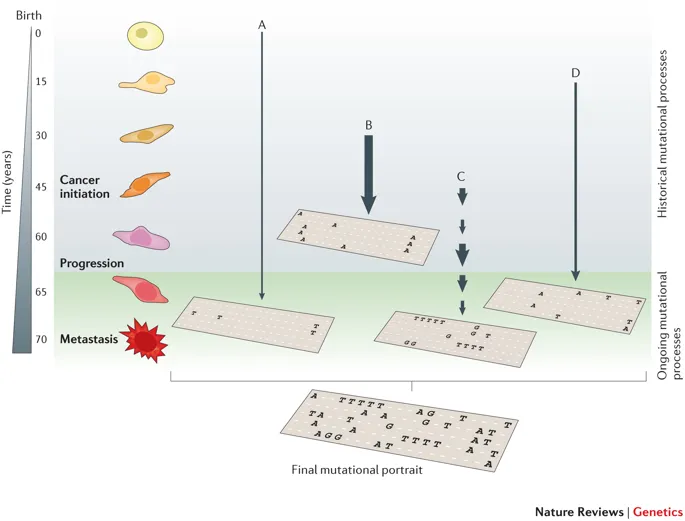
\includegraphics[width=0.8\linewidth]{fig/sbs_signature_overview_nat_review2} \caption{The illustration of SBS signature, fig source: https://www.nature.com/articles/nrg3729}\label{fig:unnamed-chunk-2}
\end{figure}

\begin{figure}
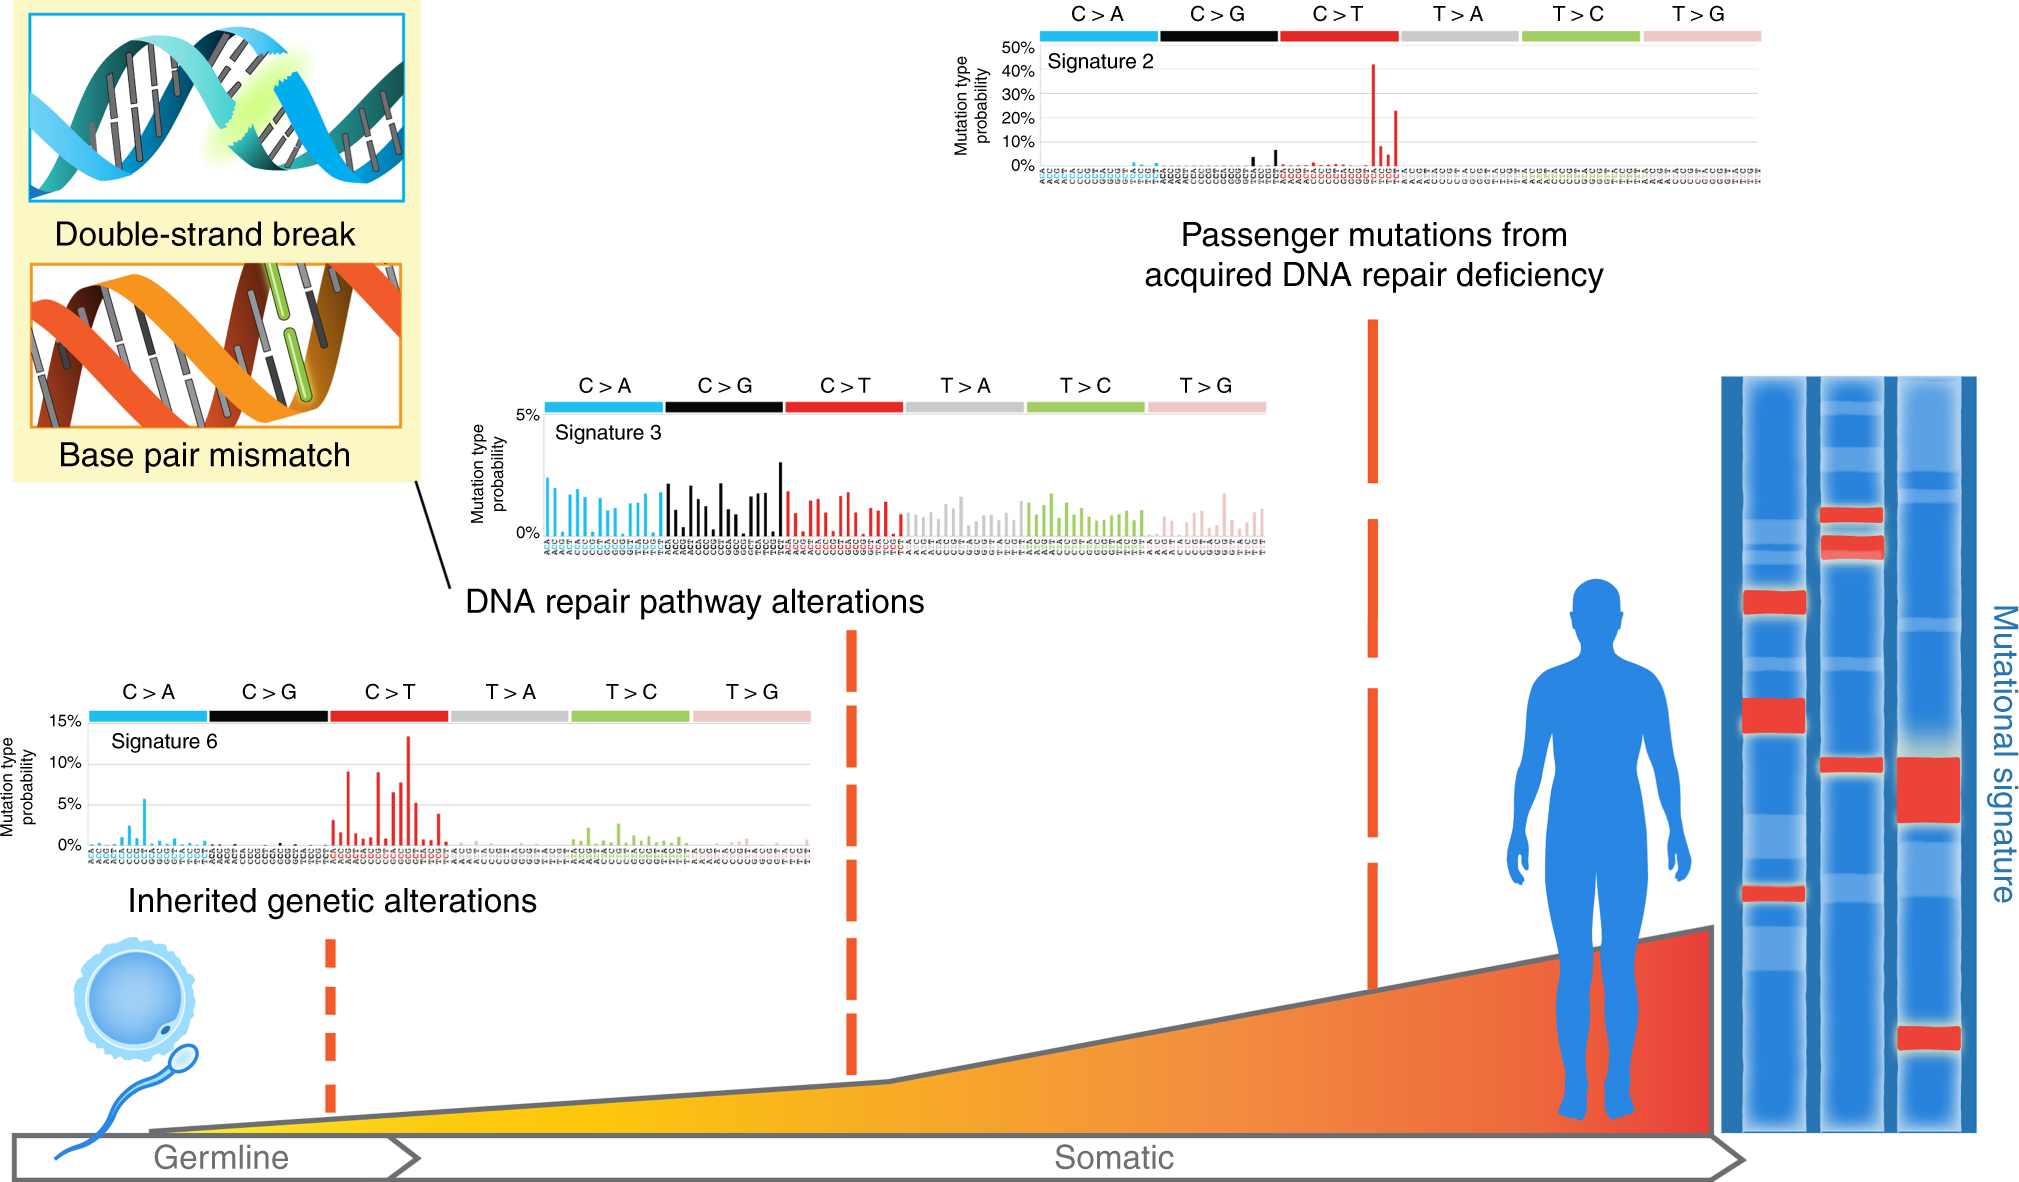
\includegraphics[width=0.95\linewidth]{fig/sbs_signature_overview} \caption{The illustration of SBS signature (2), fig source: https://www.nature.com/articles/s41467-018-05228-y}\label{fig:unnamed-chunk-3}
\end{figure}

\hypertarget{cosmic-signatures}{%
\subsection{COSMIC signatures}\label{cosmic-signatures}}

SBS (single base substitution, or SNV) signature is a famous and well-established type of mutational signature. SBS signatures are well studied and related to single-strand changes, typically caused by defective DNA repair.
Common etiologies contain aging, defective DNA mismatch repair, smoking, ultraviolet light exposure and \href{https://en.wikipedia.org/wiki/APOBEC}{APOBEC family members}.

Currently, all SBS signatures are summarized in COSMIC database, it has two versions: \href{https://cancer.sanger.ac.uk/cosmic/signatures_v2}{v2} and \href{https://cancer.sanger.ac.uk/cosmic/signatures/SBS/}{v3}.

Recently, \citet{alexandrov2020repertoire} extends the concept of mutational signature to three types of alteration: SBS, DBS (short for doublet base substitution) and INDEL (short for short insertion and deletion).
All reported common signatures are recorded in COSMIC (\url{https://cancer.sanger.ac.uk/cosmic/signatures/}), so we usually call them \textbf{COSMIC signatures}.

\textbf{SBS signatures}:

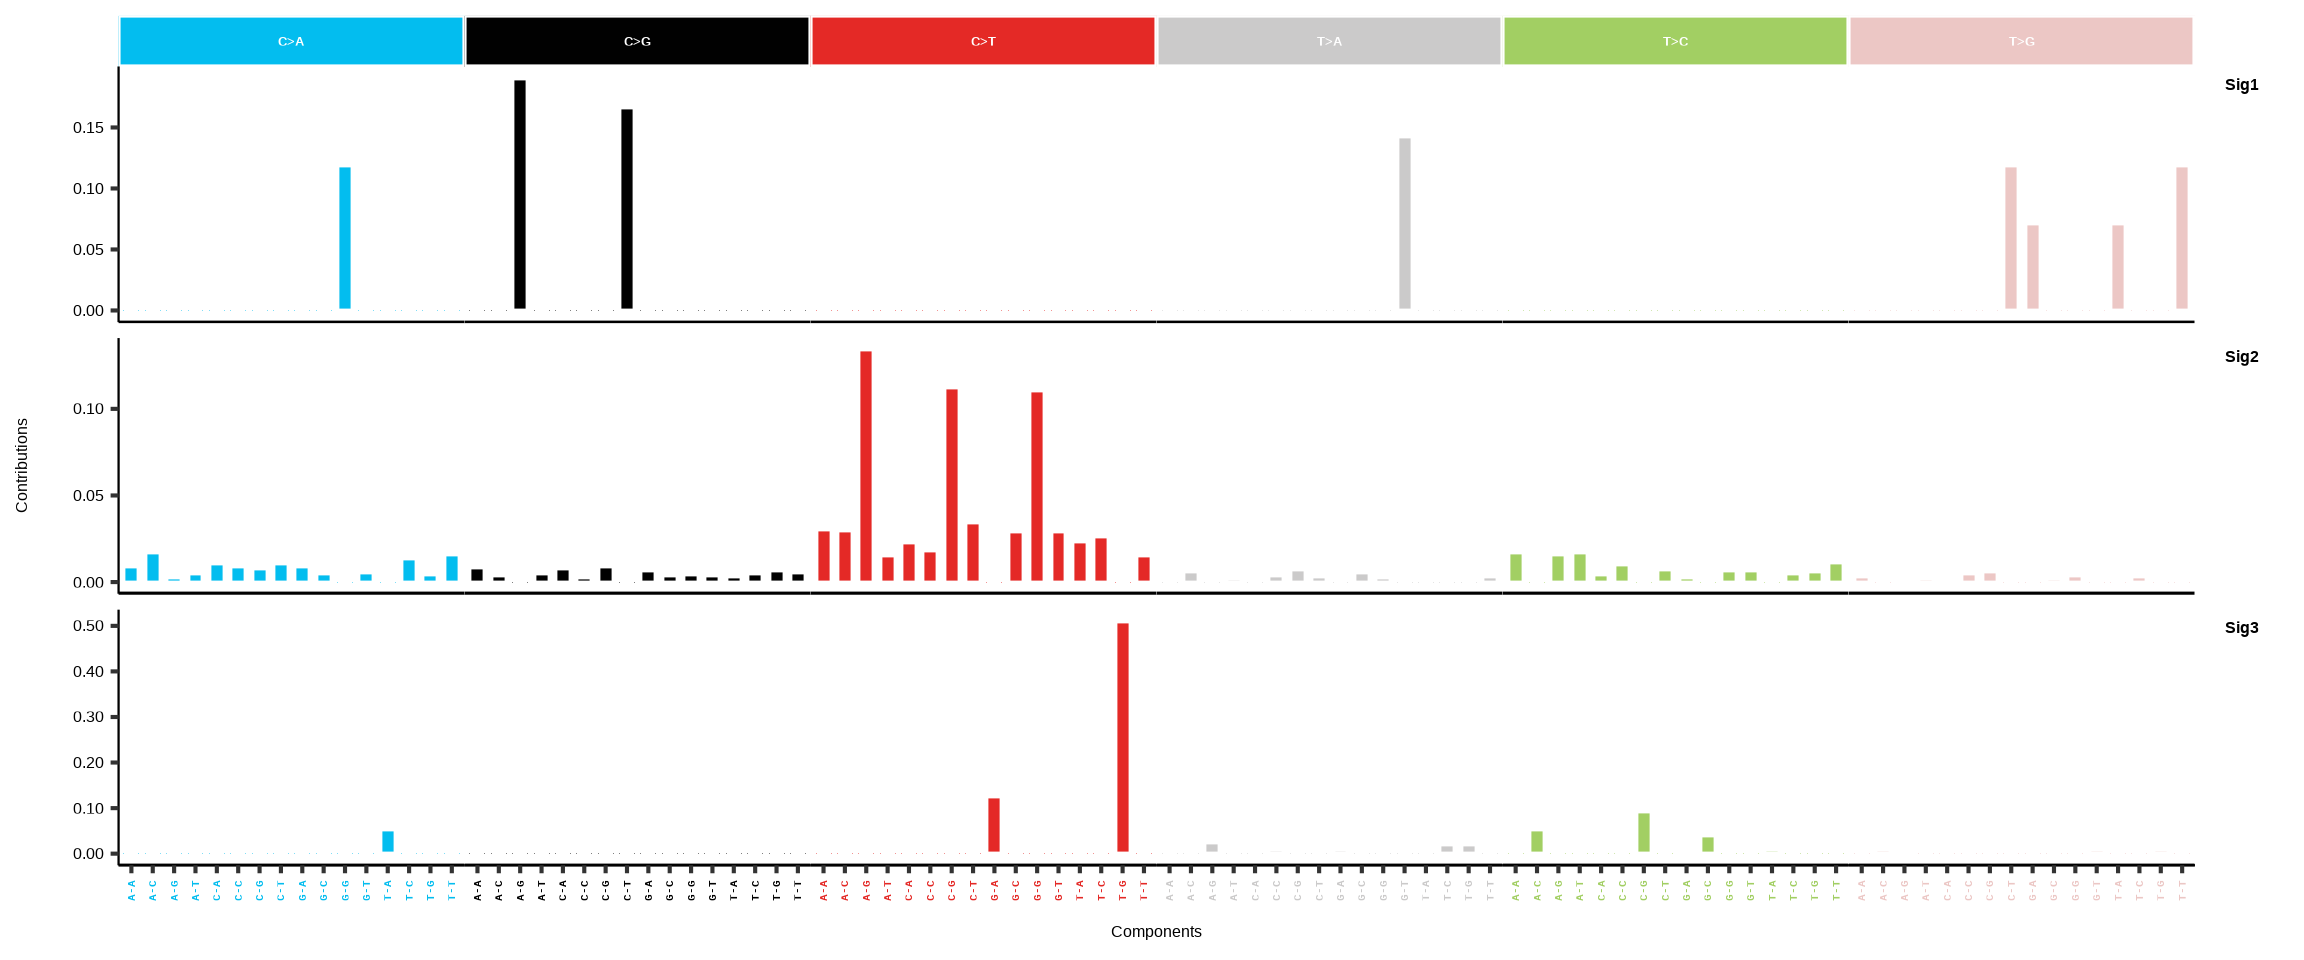
\includegraphics[width=0.95\linewidth]{sigminer_files/figure-latex/unnamed-chunk-4-1}

\textbf{DBS signatures}:

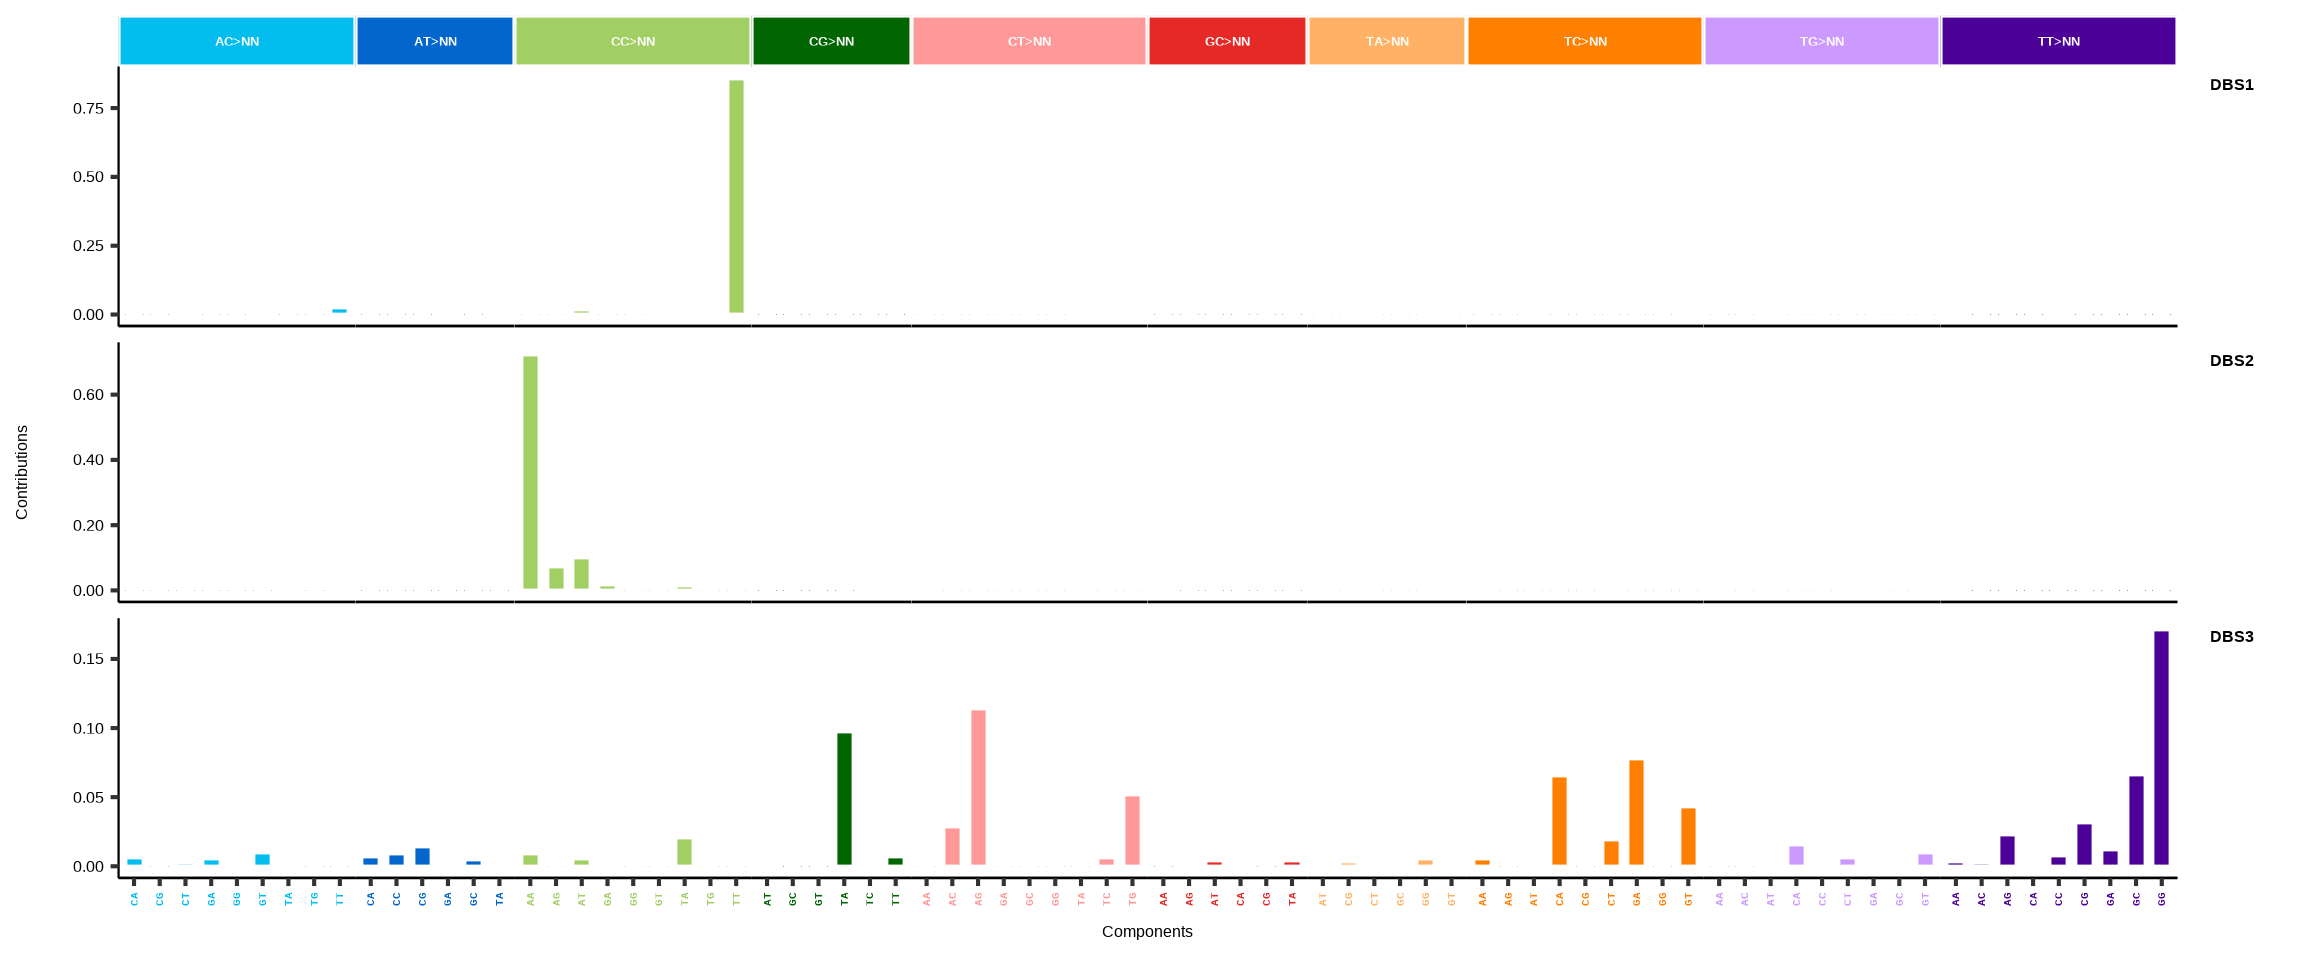
\includegraphics[width=0.95\linewidth]{sigminer_files/figure-latex/unnamed-chunk-5-1}

\textbf{INDEL (i.e.~ID) signatures}:

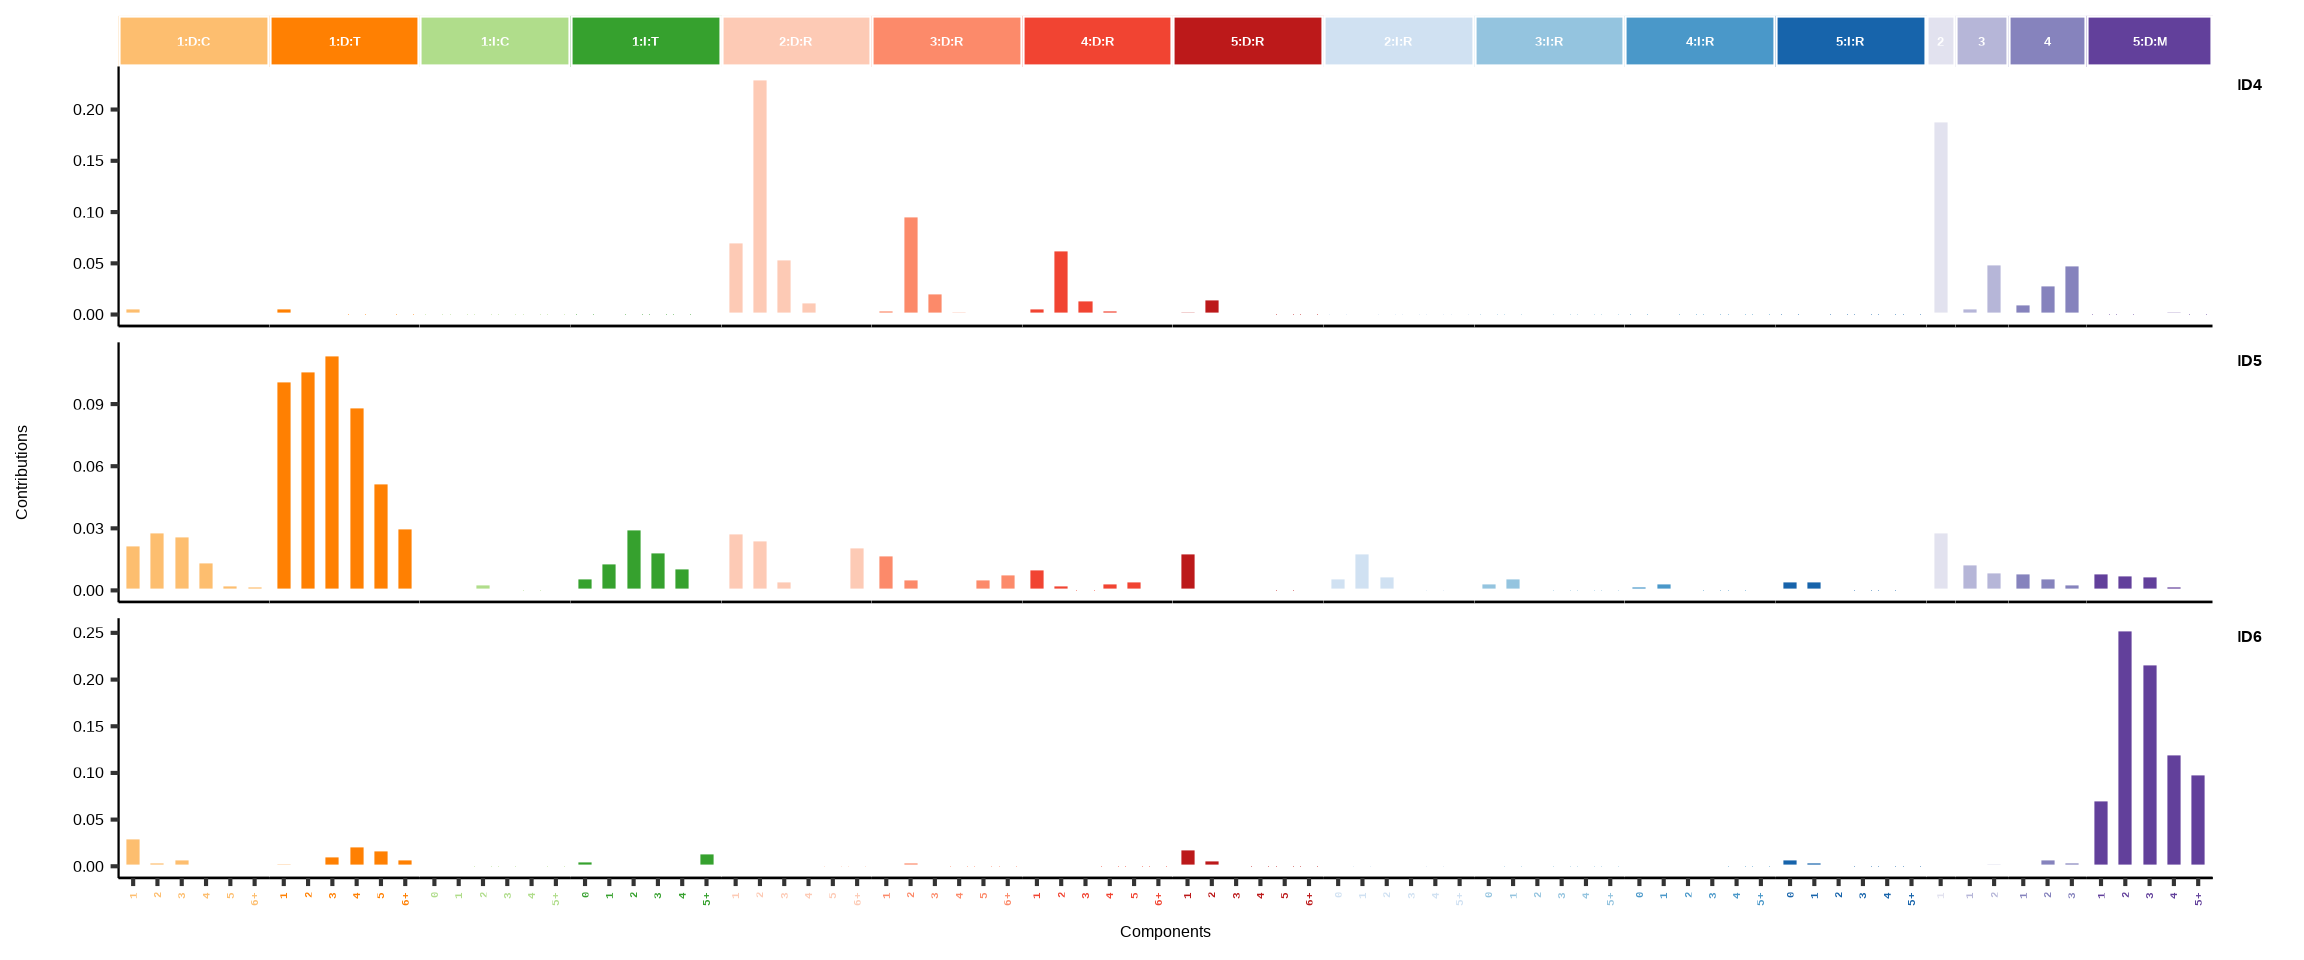
\includegraphics[width=0.95\linewidth]{sigminer_files/figure-latex/unnamed-chunk-6-1}

\hypertarget{copy-number-signatures}{%
\subsection{Copy number signatures}\label{copy-number-signatures}}

Unlike several mutation types presented in current COSMIC database for generating mutational signatures, it is hard to represent copy number features and generate the matrix for NMF decomposition.

\citet{macintyre2018copy} created a new method to generate the matrix for extracting signature by NMF algorithm. The steps are:

\begin{itemize}
\tightlist
\item
  derive 6 copy number features from absolute copy number profile
\item
  apply mixture modeling to breakdown each feature distribution into mixtures of Gaussian or mixtures of Poisson distributions
\item
  generate a sample-by-component matrix representing the sum of posterior probabilities of each copy-number event being assigned to each component.
\end{itemize}

Based on the work, we devised a new method which discards the statistical modeling and create a fixed number of predefined components from 8 copy number features to generate the matrix as the input of NMF \citep{wang2021copy},
it is easier to reproduce the result, apply to different cancer types and compare results.
To test if the method would works, we applied it to prostate cancer and successfully identified 5 copy number signatures \citep{wang2021copy}.

\begin{figure}
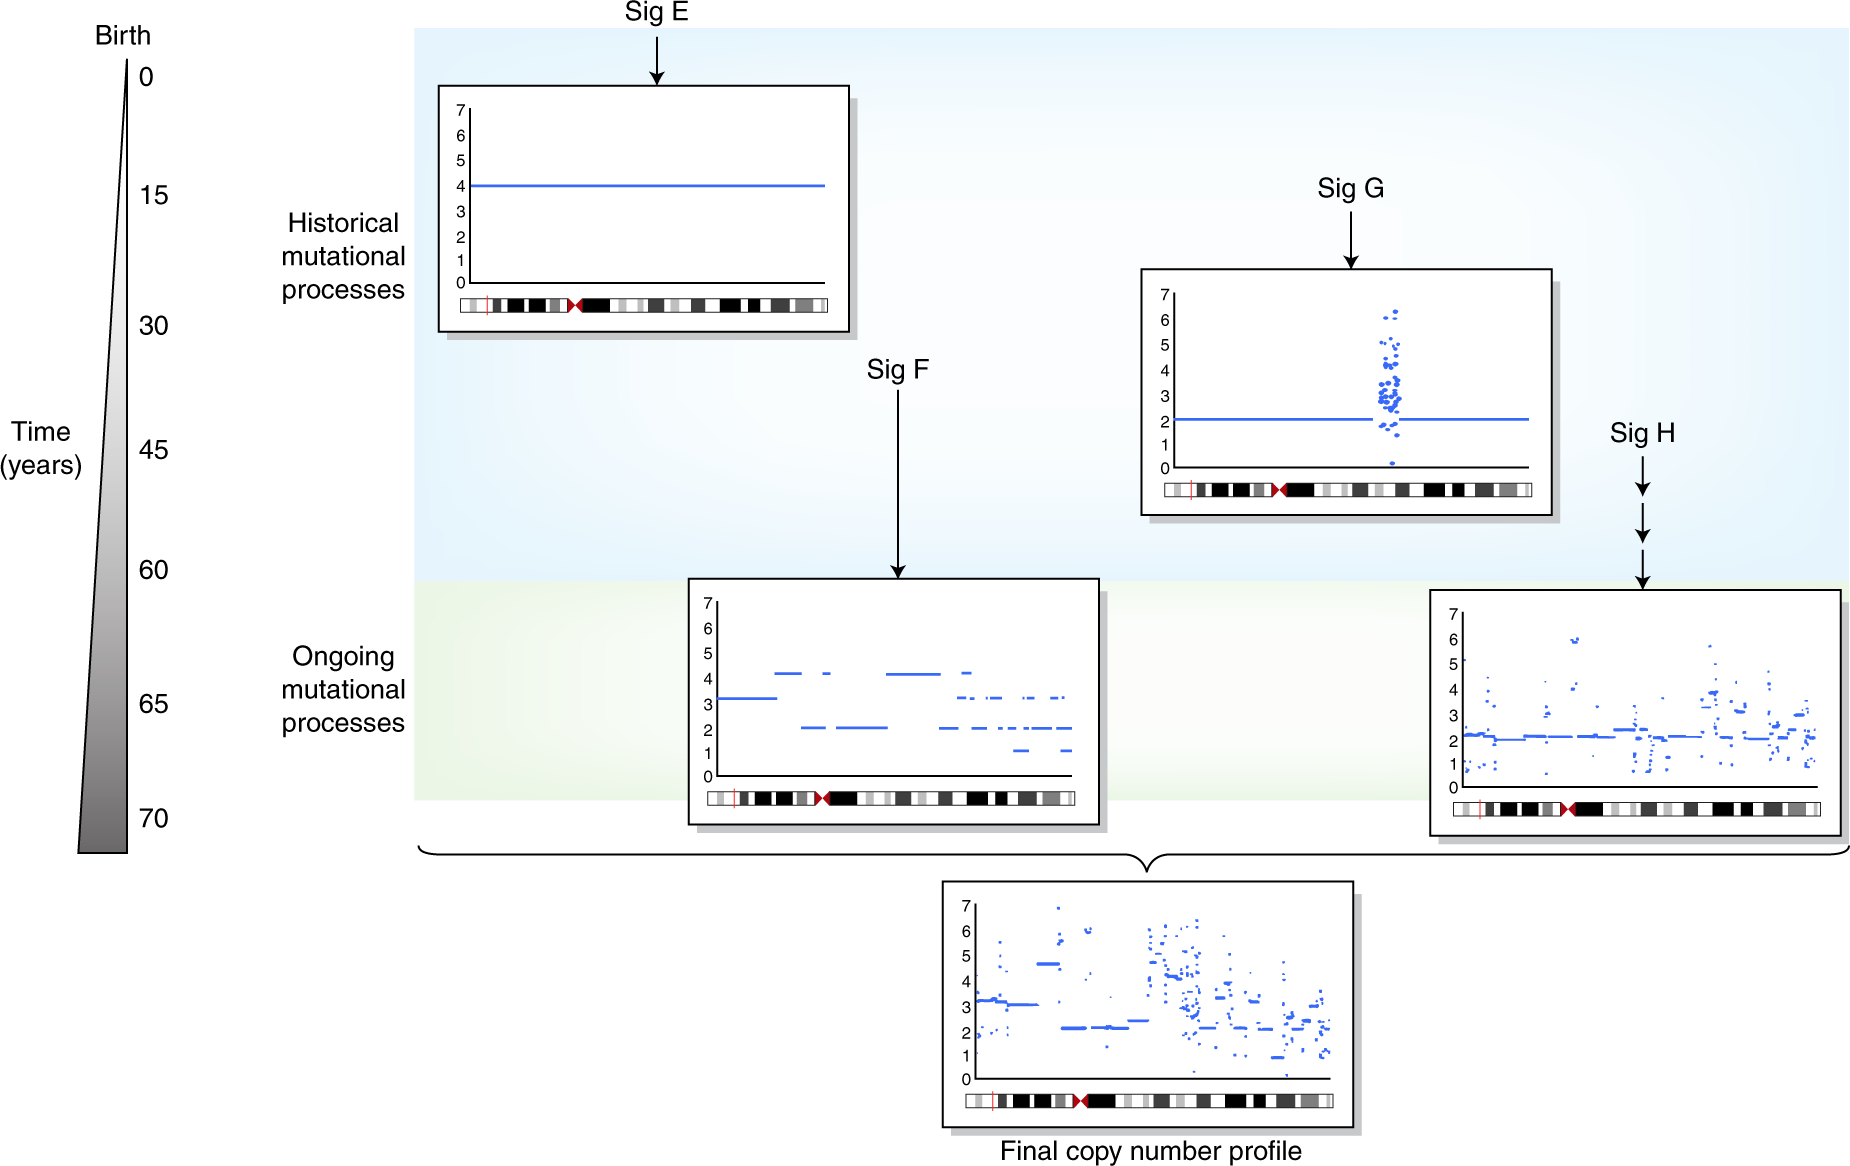
\includegraphics[width=0.95\linewidth]{fig/cn_signature_overview} \caption{The illustration of copy number signatures, fig source: https://www.nature.com/articles/s41588-018-0212-y}\label{fig:unnamed-chunk-7}
\end{figure}

Currently, there are few studies focus on copy number signatures and no reference signature database for matching and explaining the etiologies (The signatures presented in two papers above can be used as references). If you study them, you should do extra work to explore and validate them. Furthermore, the input absolute copy number data may be generated by different methods and platforms, it is normal that the contribution of some copy number feature components varies a little and result in relatively lower signature similarity when comparing different cohorts or different copy number profile generation methods.

\textbf{Copy number signatures} \emph{Wang et al} approach:

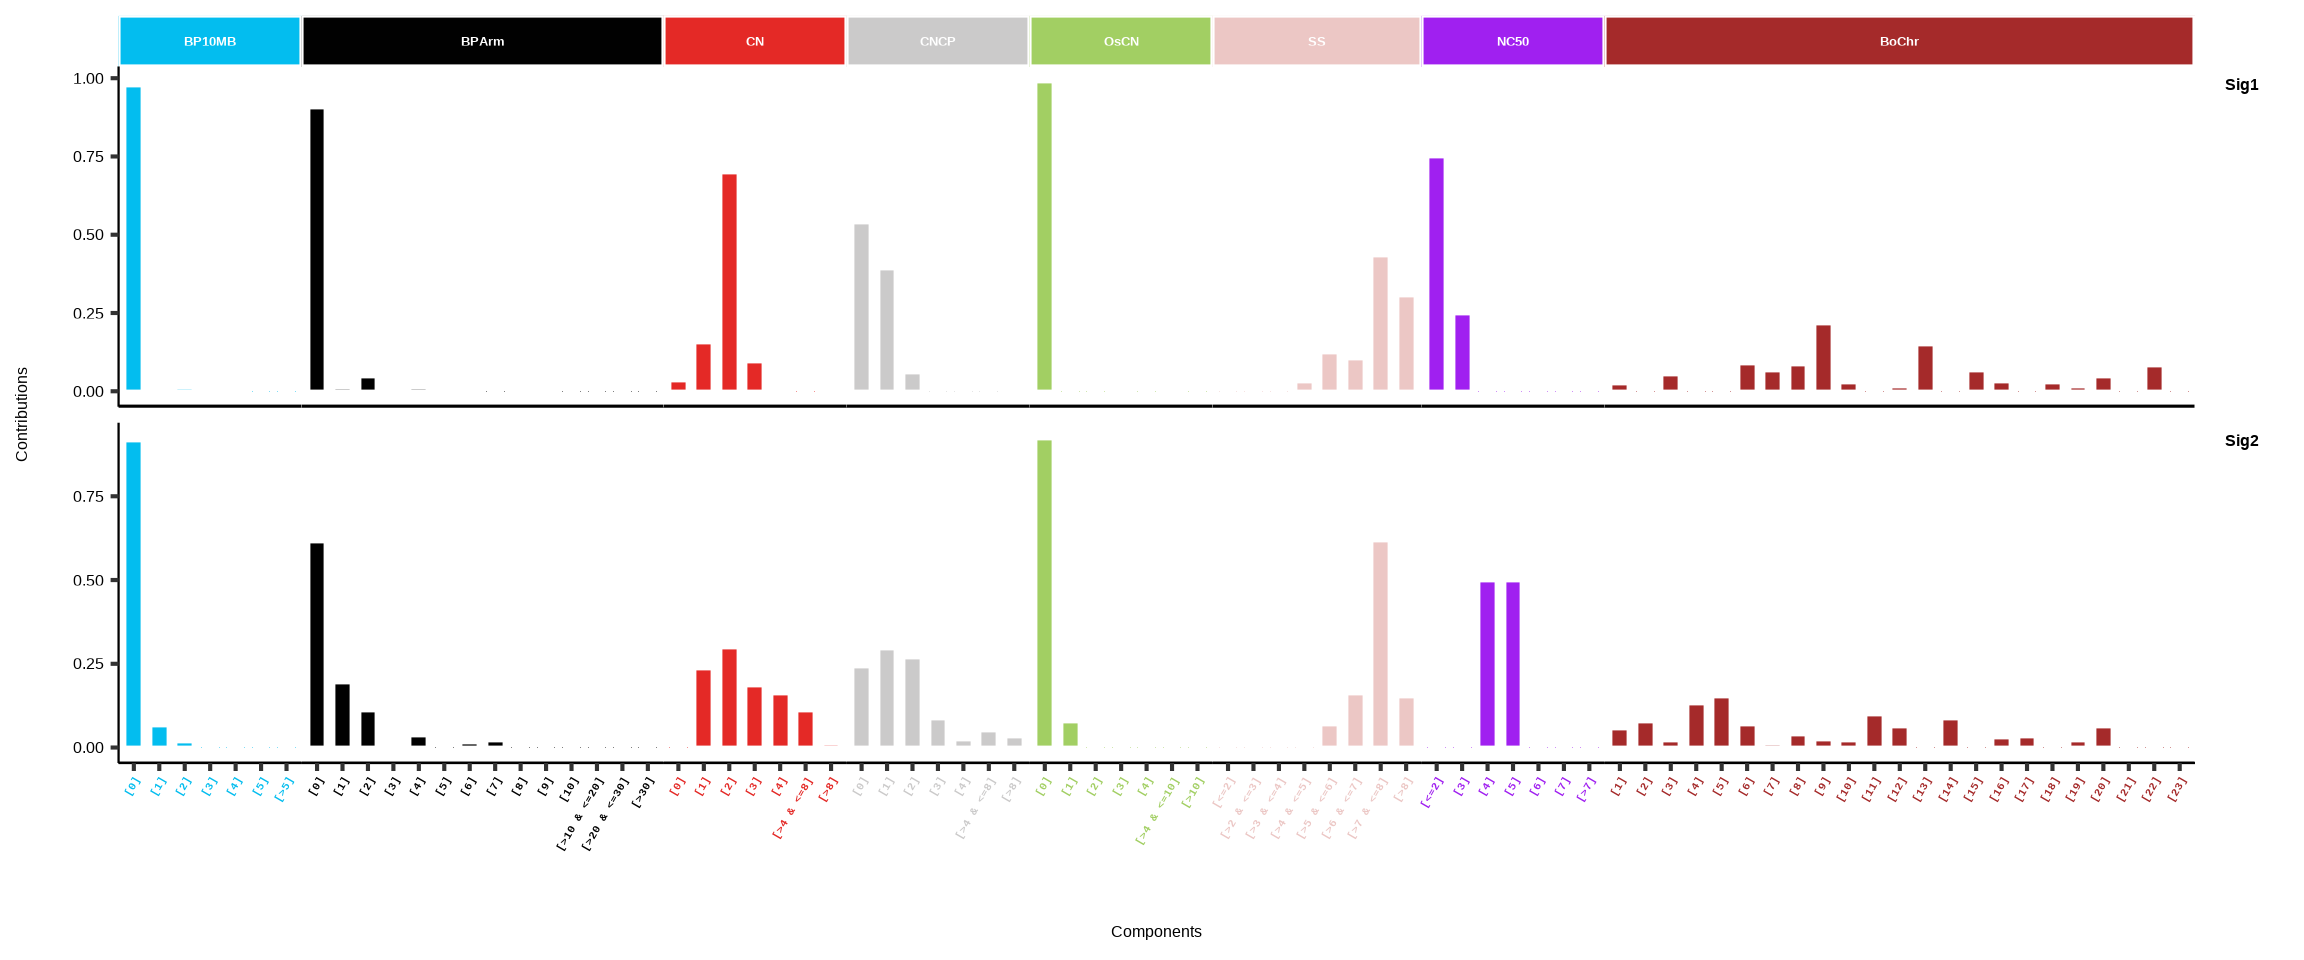
\includegraphics[width=0.95\linewidth]{sigminer_files/figure-latex/unnamed-chunk-8-1}

In addition, Alexandrov team adopted a similar approach for generating signatures like current COSMIC signatures
and described them in \textasciitilde10,000 human tumors \citep{steele2021signatures}. Many interesting results have been reported and this
would be a standard approach for allele-specific copy number profile.

\textbf{Copy number signatures} \emph{Steele et al} approach:

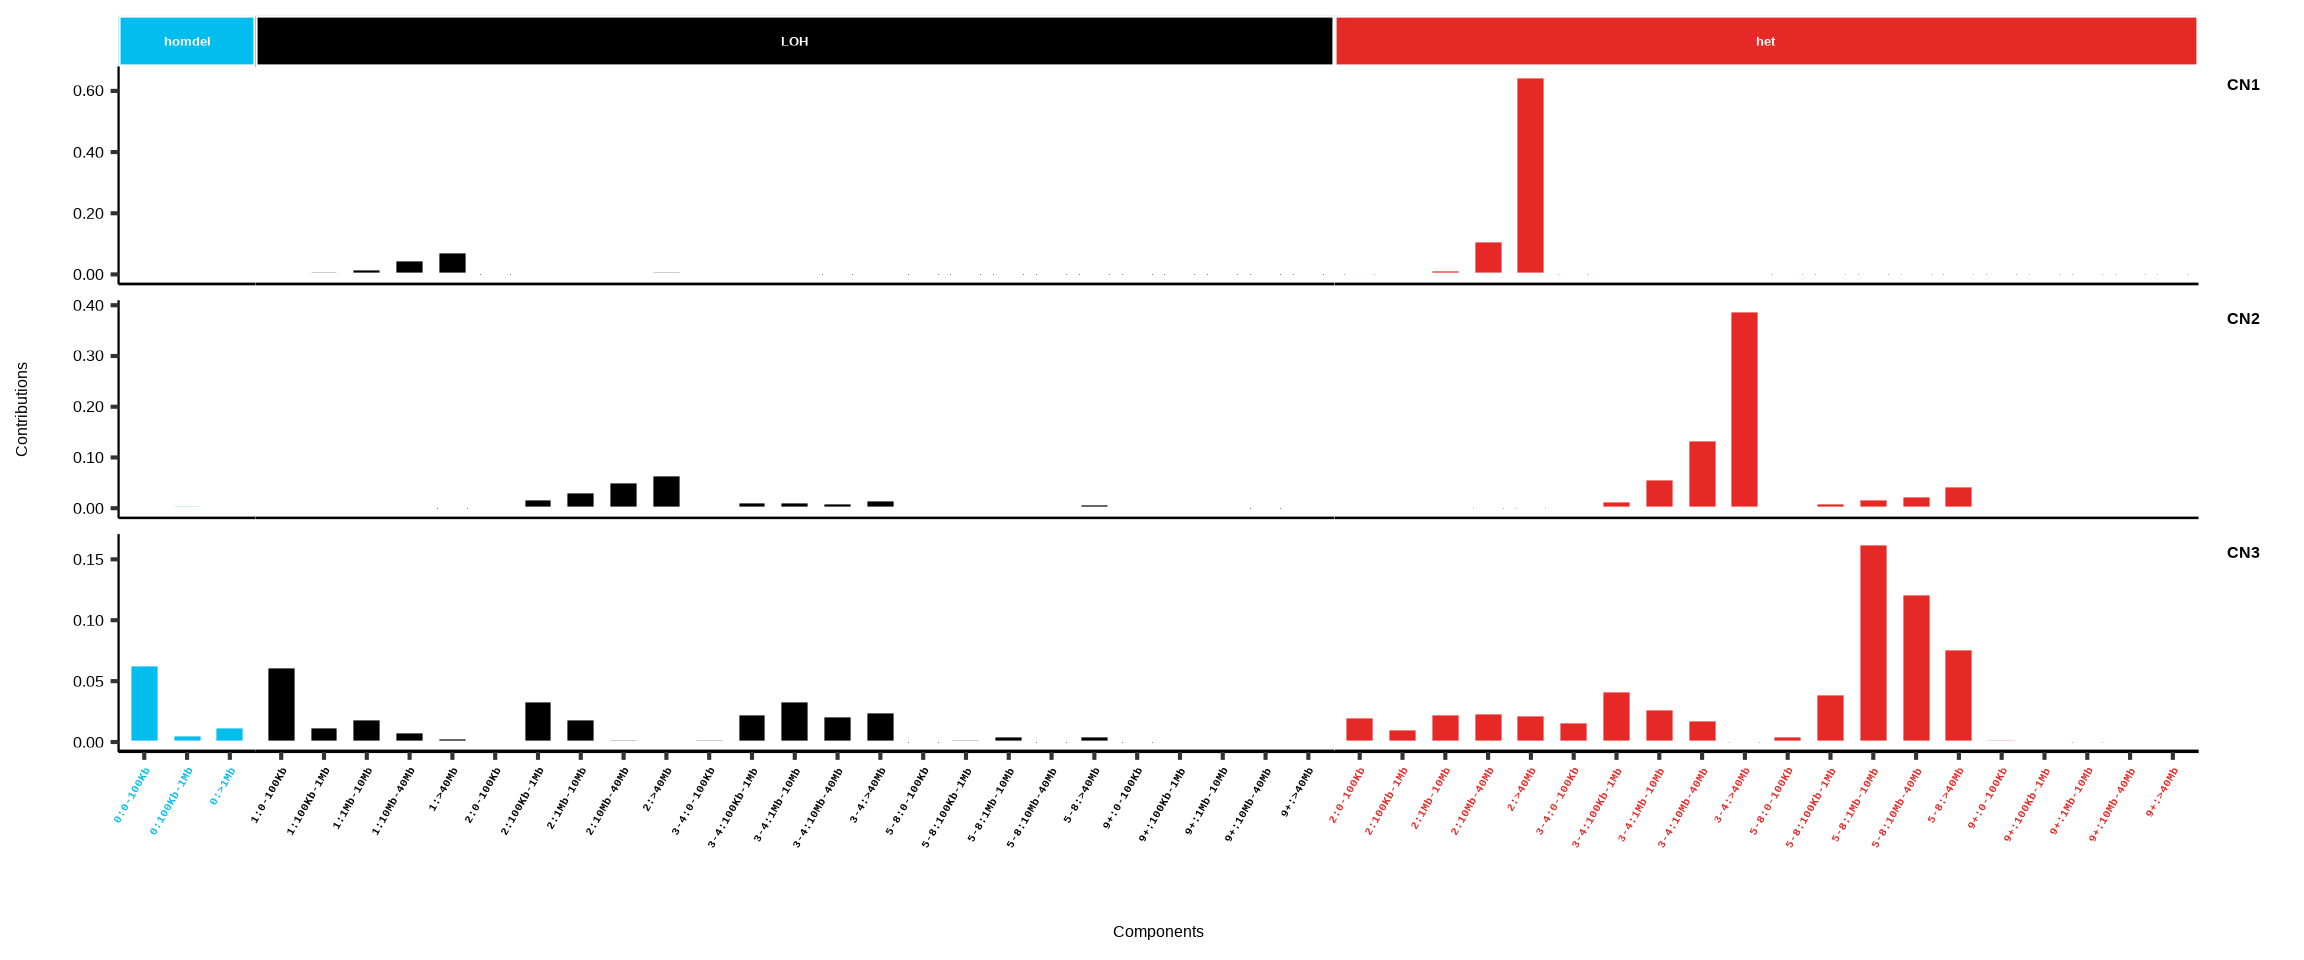
\includegraphics[width=0.95\linewidth]{sigminer_files/figure-latex/unnamed-chunk-9-1}

\hypertarget{genome-rearrangement-signatures}{%
\subsection{Genome rearrangement signatures}\label{genome-rearrangement-signatures}}

Genome rearrangement signatures (RS) also used COSMIC signature like approach to generation
rearrangement classes in each tumor sample.
RS are limited to whole genome sequencing data and also less studied.
RS has been successfully applied to 560 breast tumor WGS data \citep{nik2016landscape} and linked to clinical
outcomes in high grade serous ovarian cancers \citep{hillman2018genomic}.

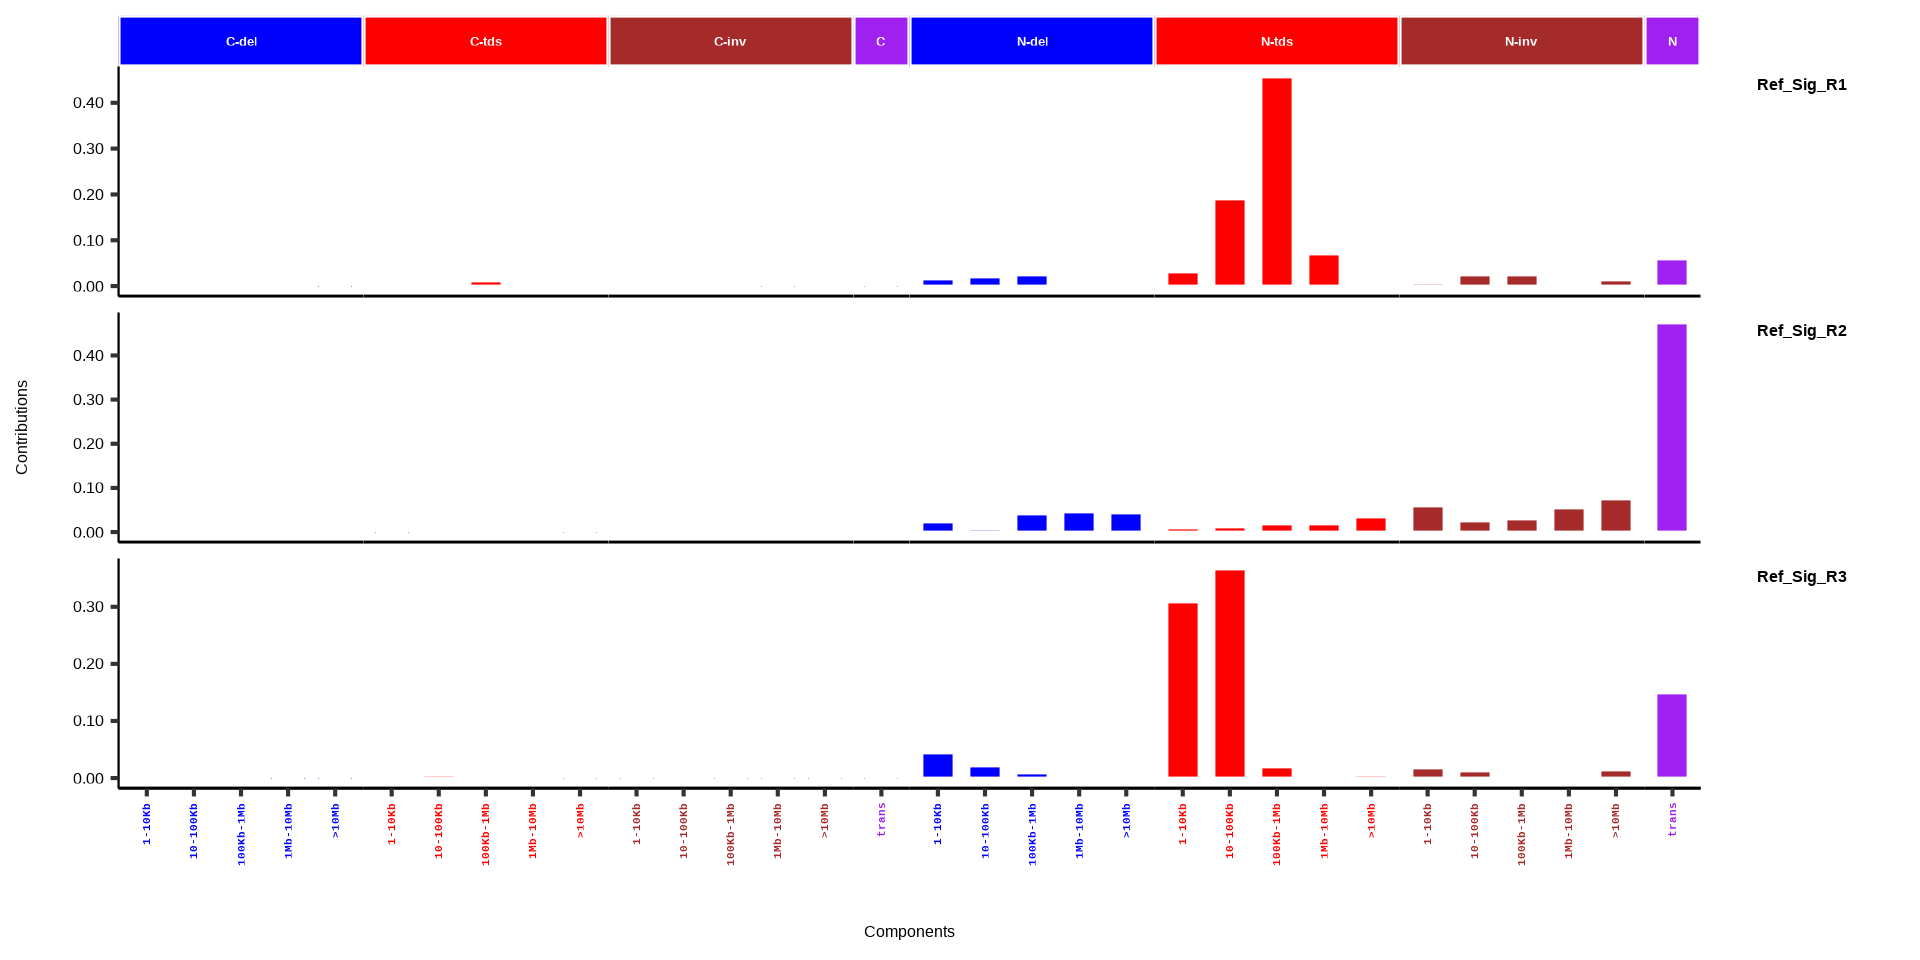
\includegraphics[width=0.95\linewidth]{sigminer_files/figure-latex/unnamed-chunk-10-1}

\hypertarget{more-information}{%
\subsection{More information}\label{more-information}}

More information about mutational signatures you can read \href{https://en.wikipedia.org/wiki/Mutational_signatures}{this wiki page}
and \href{https://cancer.sanger.ac.uk/signatures/}{COSMIC signature data page}.

\hypertarget{prerequisite}{%
\chapter{Package prerequisite and installation}\label{prerequisite}}

\hypertarget{package-prerequisite}{%
\section{Package prerequisite}\label{package-prerequisite}}

All R package dependencies of \textbf{sigminer} can be checked at \href{https://github.com/ShixiangWang/sigminer/blob/4a10d0811cb3bcb02dbbff73ed1c218954bf9b42/DESCRIPTION\#L45-L100}{specific fields of \emph{DESCRIPTION} file}.
Of note, unlike common R package, many key features of \textbf{sigminer} are only available when the suggested packages are installed.
Most of them are from \href{http://bioconductor.org/}{\emph{Bioconductor}}, so R package \textbf{BiocManager} must be installed
before installing \textbf{sigminer}. You have to use \textbf{BiocManager} instead of \texttt{install.packages()} to install \textbf{sigminer}.
If you want to handle other reference genome data except \texttt{hg19}, e.g., for \texttt{hg38}, you also have to install \emph{Bioconductor}
package \textbf{BSgenome.Hsapiens.UCSC.hg38} before/after installing \textbf{sigminer}.

\hypertarget{package-installation}{%
\section{Package installation}\label{package-installation}}

The stable release version of \textbf{sigminer} package can be installed from the CRAN:

\begin{Shaded}
\begin{Highlighting}[]
\FunctionTok{install.packages}\NormalTok{(}\StringTok{"BiocManager"}\NormalTok{)}
\NormalTok{BiocManager}\SpecialCharTok{::}\FunctionTok{install}\NormalTok{(}\StringTok{"sigminer"}\NormalTok{, }\AttributeTok{dependencies =} \ConstantTok{TRUE}\NormalTok{)}
\end{Highlighting}
\end{Shaded}

Set \texttt{dependencies\ =\ TRUE} is recommended because many packages are required for accessing full features provided by \textbf{sigminer} (we described this in previous section).
The development version of \textbf{sigminer} package can be installed from Github or Gitee after installing CRAN version \textbf{sigminer}:

\begin{Shaded}
\begin{Highlighting}[]
\FunctionTok{install.packages}\NormalTok{(}\StringTok{"remotes"}\NormalTok{)}
\CommentTok{\# From GitHub}
\NormalTok{remotes}\SpecialCharTok{::}\FunctionTok{install\_github}\NormalTok{(}\StringTok{"ShixiangWang/sigminer"}\NormalTok{, }\AttributeTok{dependencies =} \ConstantTok{TRUE}\NormalTok{)}
\CommentTok{\# From Gitee}
\NormalTok{remotes}\SpecialCharTok{::}\FunctionTok{install\_git}\NormalTok{(}\StringTok{"https://gitee.com/ShixiangWang/sigminer"}\NormalTok{, }\AttributeTok{dependencies =} \ConstantTok{TRUE}\NormalTok{)}
\end{Highlighting}
\end{Shaded}

If you see notification of package update, please keep this package up to date.

The \textbf{sigminer} is also available in Conda \emph{forge} channel. If you are using Conda,
you can install \textbf{sigminer} with:

\begin{Shaded}
\begin{Highlighting}[]
\CommentTok{\# Please note version number of the bioconda release}

\CommentTok{\# You can install an individual environment firstly with}
\CommentTok{\# conda create {-}n sigminer}
\CommentTok{\# conda activate sigminer}
\NormalTok{conda install }\SpecialCharTok{{-}}\NormalTok{c bioconda }\SpecialCharTok{{-}}\NormalTok{c conda}\SpecialCharTok{{-}}\NormalTok{forge r}\SpecialCharTok{{-}}\NormalTok{sigminer}
\end{Highlighting}
\end{Shaded}

\hypertarget{package-loading}{%
\section{Package loading}\label{package-loading}}

To load package, run:

\begin{Shaded}
\begin{Highlighting}[]
\FunctionTok{library}\NormalTok{(sigminer)}
\end{Highlighting}
\end{Shaded}

More info about \textbf{sigminer} can be given as:

\begin{Shaded}
\begin{Highlighting}[]
\FunctionTok{hello}\NormalTok{()}
\DocumentationTok{\#\# Thanks for using \textquotesingle{}sigminer\textquotesingle{} package!}
\DocumentationTok{\#\# =========================================================================}
\DocumentationTok{\#\# Version: 2.1.6}
\DocumentationTok{\#\# Run citation(\textquotesingle{}sigminer\textquotesingle{}) to see how to cite sigminer in publications.}
\DocumentationTok{\#\# }
\DocumentationTok{\#\# Project home : https://github.com/ShixiangWang/sigminer}
\DocumentationTok{\#\# Bug report   : https://github.com/ShixiangWang/sigminer/issues}
\DocumentationTok{\#\# Documentation: https://shixiangwang.github.io/sigminer{-}book/}
\DocumentationTok{\#\# =========================================================================}
\DocumentationTok{\#\# }
\end{Highlighting}
\end{Shaded}

\hypertarget{package-references}{%
\section{Package references}\label{package-references}}

All datasets/functions are well organized and documented at \href{https://shixiangwang.github.io/sigminer/reference/index.html}{package \emph{referrence} list}.
For checking usage of a specific function \texttt{fun}, you can also run \texttt{?fun} in your R console.
For example, to see usage \texttt{read\_copynumber()}

\begin{Shaded}
\begin{Highlighting}[]
\FunctionTok{library}\NormalTok{(sigminer)}
\NormalTok{?read\_copynumber}
\end{Highlighting}
\end{Shaded}

\hypertarget{part-part-ii-workflows}{%
\part*{Part II: Workflows}\label{part-part-ii-workflows}}
\addcontentsline{toc}{part}{Part II: Workflows}

\hypertarget{basic-workflow}{%
\chapter{Mutational signature analysis basics}\label{basic-workflow}}

This chapter demonstrates how to run two key mutational signature analyses (\emph{de novo} signature
discovery and signature fitting) in details.
More specifically, we will introduce how to identify COSMIC signatures from records of variant calling data.
The COSMIC signatures include three type of signatures: SBS, DBS and ID (short for INDEL). For other signature type, please read chapter \ref{analysis-supps}.

The signature identification procedure has been divided into 3 steps:

\begin{enumerate}
\def\labelenumi{\arabic{enumi}.}
\tightlist
\item
  Read mutation data.
\item
  Tally components: for SBS, it means classifying SBS records into 96 components (the most common case) and generating sample matrix by counting component in each sample.
\item
  \emph{de novo} extract signatures or quantify signature activity by fitting observed
  data to reference signature.
\end{enumerate}

\begin{itemize}
\tightlist
\item
  For \emph{de novo} signature discovery, there are manual approach and automatic approach. When you choose manual approach, you should estimate signature number and then extract specified number of signatures.
\end{itemize}

\hypertarget{data-input}{%
\section{Data input}\label{data-input}}

The input data should be in \href{https://www.ebi.ac.uk/training-beta/online/courses/human-genetic-variation-introduction/variant-identification-and-analysis/understanding-vcf-format/}{VCF}, \href{https://docs.gdc.cancer.gov/Data/File_Formats/MAF_Format/}{MAF} format.

\begin{itemize}
\tightlist
\item
  For VCF, it can only be VCF file paths.
\item
  For MAF, it can be either a MAF file or a \texttt{data.frame}.
\end{itemize}

MAF format is the standard way to represent small-scale variants in \textbf{sigminer}. There is a popular R/Bioconductor package \href{https://github.com/PoisonAlien/maftools}{\textbf{maftools}} \citep{mayakonda2018maftools} for analyzing MAF data. It provides an R class \textbf{MAF} to represent MAF format data.

\hypertarget{vcf-as-input}{%
\subsection{VCF as input}\label{vcf-as-input}}

If you use VCF files as input, you can use \texttt{read\_vcf()} to read multiple VCF files as a \texttt{MAF} object.

\begin{Shaded}
\begin{Highlighting}[]
\FunctionTok{library}\NormalTok{(sigminer)}

\NormalTok{vcfs }\OtherTok{\textless{}{-}} \FunctionTok{list.files}\NormalTok{(}\FunctionTok{system.file}\NormalTok{(}\StringTok{"extdata"}\NormalTok{, }\AttributeTok{package =} \StringTok{"sigminer"}\NormalTok{), }\StringTok{"*.vcf"}\NormalTok{, }\AttributeTok{full.names =} \ConstantTok{TRUE}\NormalTok{)}
\NormalTok{maf }\OtherTok{\textless{}{-}} \FunctionTok{read\_vcf}\NormalTok{(vcfs)}
\DocumentationTok{\#\# Reading file(s): /Users/wsx/Library/R/sigminer/extdata/test1.vcf, /Users/wsx/Library/R/sigminer/extdata/test2.vcf, /Users/wsx/Library/R/sigminer/extdata/test3.vcf}
\DocumentationTok{\#\# It seems /Users/wsx/Library/R/sigminer/extdata/test2.vcf has no normal VCF header, try parsing without header.}
\DocumentationTok{\#\# Annotating Variant Type...}
\DocumentationTok{\#\# Downloading https://zenodo.org/record/4771552/files/human\_hg19\_gene\_info.rds to /Users/wsx/Library/R/sigminer/extdata/human\_hg19\_gene\_info.rds}
\DocumentationTok{\#\# Annotating mutations to first matched gene based on database /Users/wsx/Library/R/sigminer/extdata/human\_hg19\_gene\_info.rds...}
\DocumentationTok{\#\# Transforming into a MAF object...}
\DocumentationTok{\#\# {-}Validating}
\DocumentationTok{\#\# {-}{-}Non MAF specific values in Variant\_Classification column:}
\DocumentationTok{\#\#   Unknown}
\DocumentationTok{\#\# {-}Summarizing}
\DocumentationTok{\#\# {-}Processing clinical data}
\DocumentationTok{\#\# {-}{-}Missing clinical data}
\DocumentationTok{\#\# {-}Finished in 0.064s elapsed (0.055s cpu)}
\NormalTok{maf }\OtherTok{\textless{}{-}} \FunctionTok{read\_vcf}\NormalTok{(vcfs, }\AttributeTok{keep\_only\_pass =} \ConstantTok{FALSE}\NormalTok{)}
\DocumentationTok{\#\# Reading file(s): /Users/wsx/Library/R/sigminer/extdata/test1.vcf, /Users/wsx/Library/R/sigminer/extdata/test2.vcf, /Users/wsx/Library/R/sigminer/extdata/test3.vcf}
\DocumentationTok{\#\# It seems /Users/wsx/Library/R/sigminer/extdata/test2.vcf has no normal VCF header, try parsing without header.}
\DocumentationTok{\#\# Annotating Variant Type...}
\DocumentationTok{\#\# Annotating mutations to first matched gene based on database /Users/wsx/Library/R/sigminer/extdata/human\_hg19\_gene\_info.rds...}
\DocumentationTok{\#\# Transforming into a MAF object...}
\DocumentationTok{\#\# {-}Validating}
\DocumentationTok{\#\# {-}{-}Non MAF specific values in Variant\_Classification column:}
\DocumentationTok{\#\#   Unknown}
\DocumentationTok{\#\# {-}Summarizing}
\DocumentationTok{\#\# {-}Processing clinical data}
\DocumentationTok{\#\# {-}{-}Missing clinical data}
\DocumentationTok{\#\# {-}Finished in 0.043s elapsed (0.043s cpu)}
\end{Highlighting}
\end{Shaded}

\hypertarget{maf-as-input}{%
\subsection{MAF as input}\label{maf-as-input}}

MAF format is the most recommended input, you can provide it either as a file or as a \texttt{data.frame}.

Typically, you can obtain the data in the following ways:

\begin{enumerate}
\def\labelenumi{\arabic{enumi}.}
\tightlist
\item
  You get multiple VCF files and convert them into a MAF file (\href{https://github.com/mskcc/vcf2maf}{vcf2maf} is the most used tool for conversion).
\item
  You get a MAF file from a reference or a public data portal, e.g., \href{http://www.cbioportal.org/}{cBioPortal} or \href{https://portal.gdc.cancer.gov/}{GDC portal}.
\item
  You get a EXCEL file providing MAF-like data from a reference, you should read the data firstly (with \texttt{readxl::read\_excel()}) and then construct a \texttt{data.frame} providing necessary columns.
\end{enumerate}

Once a MAF file or a MAF-like \texttt{data.frame} is ready, you can read/convert it as a \texttt{MAF} object with \texttt{read\_maf()}. Here TCGA LAML dataset is used as an example:

\begin{Shaded}
\begin{Highlighting}[]
\NormalTok{laml.maf }\OtherTok{\textless{}{-}} \FunctionTok{system.file}\NormalTok{(}\StringTok{"extdata"}\NormalTok{, }\StringTok{"tcga\_laml.maf.gz"}\NormalTok{, }\AttributeTok{package =} \StringTok{"maftools"}\NormalTok{, }\AttributeTok{mustWork =} \ConstantTok{TRUE}\NormalTok{)}
\NormalTok{laml }\OtherTok{\textless{}{-}} \FunctionTok{read\_maf}\NormalTok{(}\AttributeTok{maf =}\NormalTok{ laml.maf)}
\DocumentationTok{\#\# {-}Reading}
\DocumentationTok{\#\# {-}Validating}
\DocumentationTok{\#\# {-}Silent variants: 475 }
\DocumentationTok{\#\# {-}Summarizing}
\DocumentationTok{\#\# {-}Processing clinical data}
\DocumentationTok{\#\# {-}{-}Missing clinical data}
\DocumentationTok{\#\# {-}Finished in 0.443s elapsed (0.414s cpu)}
\NormalTok{laml}
\DocumentationTok{\#\# An object of class  MAF }
\DocumentationTok{\#\#                    ID          summary  Mean Median}
\DocumentationTok{\#\#  1:        NCBI\_Build               37    NA     NA}
\DocumentationTok{\#\#  2:            Center genome.wustl.edu    NA     NA}
\DocumentationTok{\#\#  3:           Samples              193    NA     NA}
\DocumentationTok{\#\#  4:            nGenes             1241    NA     NA}
\DocumentationTok{\#\#  5:   Frame\_Shift\_Del               52 0.269      0}
\DocumentationTok{\#\#  6:   Frame\_Shift\_Ins               91 0.472      0}
\DocumentationTok{\#\#  7:      In\_Frame\_Del               10 0.052      0}
\DocumentationTok{\#\#  8:      In\_Frame\_Ins               42 0.218      0}
\DocumentationTok{\#\#  9: Missense\_Mutation             1342 6.953      7}
\DocumentationTok{\#\# 10: Nonsense\_Mutation              103 0.534      0}
\DocumentationTok{\#\# 11:       Splice\_Site               92 0.477      0}
\DocumentationTok{\#\# 12:             total             1732 8.974      9}
\end{Highlighting}
\end{Shaded}

The \texttt{laml} is a \texttt{MAF} object. The \texttt{MAF} class is exported from \textbf{maftools} to \textbf{sigminer}. So \texttt{laml} can be directly use functions provided by \textbf{maftools}.

As a \texttt{MAF} object, the mutation records are stored in slot \texttt{data} and \texttt{maf.silent}.

\begin{Shaded}
\begin{Highlighting}[]
\FunctionTok{head}\NormalTok{(laml}\SpecialCharTok{@}\NormalTok{data)}
\DocumentationTok{\#\#    Hugo\_Symbol Entrez\_Gene\_Id           Center NCBI\_Build Chromosome}
\DocumentationTok{\#\# 1:      ABCA10          10349 genome.wustl.edu         37         17}
\DocumentationTok{\#\# 2:       ABCA4             24 genome.wustl.edu         37          1}
\DocumentationTok{\#\# 3:      ABCB11           8647 genome.wustl.edu         37          2}
\DocumentationTok{\#\# 4:       ABCC3           8714 genome.wustl.edu         37         17}
\DocumentationTok{\#\# 5:       ABCF1             23 genome.wustl.edu         37          6}
\DocumentationTok{\#\# 6:       ABCG4          64137 genome.wustl.edu         37         11}
\DocumentationTok{\#\#    Start\_Position End\_Position Strand Variant\_Classification Variant\_Type}
\DocumentationTok{\#\# 1:       67170917     67170917      +            Splice\_Site          SNP}
\DocumentationTok{\#\# 2:       94490594     94490594      +      Missense\_Mutation          SNP}
\DocumentationTok{\#\# 3:      169780250    169780250      +      Missense\_Mutation          SNP}
\DocumentationTok{\#\# 4:       48760974     48760974      +      Missense\_Mutation          SNP}
\DocumentationTok{\#\# 5:       30554429     30554429      +      Missense\_Mutation          SNP}
\DocumentationTok{\#\# 6:      119031351    119031351      +      Missense\_Mutation          SNP}
\DocumentationTok{\#\#    Reference\_Allele Tumor\_Seq\_Allele1 Tumor\_Seq\_Allele2 Tumor\_Sample\_Barcode}
\DocumentationTok{\#\# 1:                T                 T                 C         TCGA{-}AB{-}2988}
\DocumentationTok{\#\# 2:                C                 C                 T         TCGA{-}AB{-}2869}
\DocumentationTok{\#\# 3:                G                 G                 A         TCGA{-}AB{-}3009}
\DocumentationTok{\#\# 4:                C                 C                 T         TCGA{-}AB{-}2887}
\DocumentationTok{\#\# 5:                G                 G                 A         TCGA{-}AB{-}2920}
\DocumentationTok{\#\# 6:                A                 A                 G         TCGA{-}AB{-}2934}
\DocumentationTok{\#\#    Protein\_Change i\_TumorVAF\_WU i\_transcript\_name}
\DocumentationTok{\#\# 1:        p.K960R      45.66000       NM\_080282.3}
\DocumentationTok{\#\# 2:       p.R1517H      38.12000       NM\_000350.2}
\DocumentationTok{\#\# 3:       p.A1283V      46.97218       NM\_003742.2}
\DocumentationTok{\#\# 4:       p.P1271S      56.41000       NM\_003786.1}
\DocumentationTok{\#\# 5:        p.G658S      40.95000    NM\_001025091.1}
\DocumentationTok{\#\# 6:        p.Y567C      32.84000       NM\_022169.1}
\FunctionTok{head}\NormalTok{(laml}\SpecialCharTok{@}\NormalTok{maf.silent)}
\DocumentationTok{\#\#    Hugo\_Symbol Entrez\_Gene\_Id           Center NCBI\_Build Chromosome}
\DocumentationTok{\#\# 1:      ABCC11          85320 genome.wustl.edu         37         16}
\DocumentationTok{\#\# 2:        ACAN            176 genome.wustl.edu         37         15}
\DocumentationTok{\#\# 3:       ACAT1             38 genome.wustl.edu         37         11}
\DocumentationTok{\#\# 4:       ACCN2             41 genome.wustl.edu         37         12}
\DocumentationTok{\#\# 5:       ACTA2             59 genome.wustl.edu         37         10}
\DocumentationTok{\#\# 6:       ACTL9         284382 genome.wustl.edu         37         19}
\DocumentationTok{\#\#    Start\_Position End\_Position Strand Variant\_Classification Variant\_Type}
\DocumentationTok{\#\# 1:       48244997     48244997      +                 Silent          SNP}
\DocumentationTok{\#\# 2:       89401084     89401084      +                 Silent          SNP}
\DocumentationTok{\#\# 3:      108009744    108009744      +                 Silent          SNP}
\DocumentationTok{\#\# 4:       50452780     50452780      +                 Silent          SNP}
\DocumentationTok{\#\# 5:       90695109     90695109      +                 Silent          SNP}
\DocumentationTok{\#\# 6:        8808551      8808551      +                 Silent          SNP}
\DocumentationTok{\#\#    Reference\_Allele Tumor\_Seq\_Allele1 Tumor\_Seq\_Allele2 Tumor\_Sample\_Barcode}
\DocumentationTok{\#\# 1:                G                 G                 A         TCGA{-}AB{-}2830}
\DocumentationTok{\#\# 2:                C                 C                 T         TCGA{-}AB{-}2898}
\DocumentationTok{\#\# 3:                T                 T                 G         TCGA{-}AB{-}2887}
\DocumentationTok{\#\# 4:                C                 C                 G         TCGA{-}AB{-}3009}
\DocumentationTok{\#\# 5:                C                 C                 T         TCGA{-}AB{-}2973}
\DocumentationTok{\#\# 6:                G                 G                 A         TCGA{-}AB{-}2936}
\DocumentationTok{\#\#    Protein\_Change i\_TumorVAF\_WU i\_transcript\_name}
\DocumentationTok{\#\# 1:        p.I490I    34.2700000       NM\_032583.3}
\DocumentationTok{\#\# 2:       p.S1756S    38.3000000       NM\_013227.2}
\DocumentationTok{\#\# 3:        p.T185T    49.0400000       NM\_000019.3}
\DocumentationTok{\#\# 4:         p.L77L    48.1000000       NM\_020039.2}
\DocumentationTok{\#\# 5:        p.P335P     0.2012072       NM\_001613.1}
\DocumentationTok{\#\# 6:        p.F167F    46.1500000       NM\_178525.3}
\end{Highlighting}
\end{Shaded}

The \texttt{data} slot contains non-silent variants, and the \texttt{maf.silent} slot contains silent variants.
Default uses ``Variant Classifications'' with high/moderate variant consequences as non-silent variants. \url{http://asia.ensembl.org/Help/Glossary?id=535}: ``Frame\_Shift\_Del'', ``Frame\_Shift\_Ins'', ``Splice\_Site'', ``Translation\_Start\_Site'',``Nonsense\_Mutation'', ``Nonstop\_Mutation'', ``In\_Frame\_Del'',``In\_Frame\_Ins'', ``Missense\_Mutation'' (see \texttt{?read\_maf}). If you want to change, please set \texttt{vc\_nonSyn} option.

Other slots in \texttt{MAF} object are summary data either by sample or gene/variant type etc.

\begin{Shaded}
\begin{Highlighting}[]
\FunctionTok{slotNames}\NormalTok{(laml)}
\DocumentationTok{\#\# [1] "data"                           "variants.per.sample"           }
\DocumentationTok{\#\# [3] "variant.type.summary"           "variant.classification.summary"}
\DocumentationTok{\#\# [5] "gene.summary"                   "summary"                       }
\DocumentationTok{\#\# [7] "maf.silent"                     "clinical.data"}
\end{Highlighting}
\end{Shaded}

Acute myeloid leukemia is not a good object to study mutational signatures due to low mutation burden, we will use a subset of TCGA breast cohort as for illustration of the following analyses.

Anand Mayakonda has already stored whole TCGA mutation data as MAF objects in \href{https://github.com/PoisonAlien/TCGAmutations}{\textbf{TCGAmutations}} package.
Here I will load the TCGA BRCA cohort and create a sub-cohort with 100 tumors.

\begin{Shaded}
\begin{Highlighting}[]
\FunctionTok{library}\NormalTok{(maftools)}
\FunctionTok{tcgaAvailable}\NormalTok{()}
\end{Highlighting}
\end{Shaded}

\begin{Shaded}
\begin{Highlighting}[]
\FunctionTok{set.seed}\NormalTok{(}\DecValTok{1234}\NormalTok{)}
\CommentTok{\# brca \textless{}{-} readRDS("data/BRCA.RDs")}
\NormalTok{brca }\OtherTok{\textless{}{-}} \FunctionTok{tcga\_load}\NormalTok{(}\StringTok{"BRCA"}\NormalTok{)}
\NormalTok{brca }\OtherTok{\textless{}{-}} \FunctionTok{subsetMaf}\NormalTok{(brca,}
  \AttributeTok{tsb =} \FunctionTok{as.character}\NormalTok{(}\FunctionTok{sample}\NormalTok{(brca}\SpecialCharTok{@}\NormalTok{variants.per.sample}\SpecialCharTok{$}\NormalTok{Tumor\_Sample\_Barcode, }\DecValTok{100}\NormalTok{))}
\NormalTok{)}
\FunctionTok{saveRDS}\NormalTok{(brca, }\AttributeTok{file =} \StringTok{"data/brca.rds"}\NormalTok{)}
\end{Highlighting}
\end{Shaded}

\begin{quote}
Here we save this cohort so no need to download the dataset every time.
\end{quote}

\begin{Shaded}
\begin{Highlighting}[]
\NormalTok{brca }\OtherTok{\textless{}{-}} \FunctionTok{readRDS}\NormalTok{(}\StringTok{"data/brca.rds"}\NormalTok{)}
\end{Highlighting}
\end{Shaded}

For CNV and genome rearrangement records, check chapter \ref{analysis-supps}.

\hypertarget{tally-components}{%
\section{Tally components}\label{tally-components}}

\hypertarget{the-most-common-96-components}{%
\subsection{The most common 96 components}\label{the-most-common-96-components}}

According to 3-nucleotide context (mutated base, 5' and 3' adjacent bases) and base complementary pairing principle, we can divide all SBS mutations into 96 mutation types. We call each mutation type as a \emph{component} here.

\begin{quote}
This classification is based the six substitution subtypes: C\textgreater A, C\textgreater G, C\textgreater T, T\textgreater A, T\textgreater C, and T\textgreater G (all substitutions are referred to by the pyrimidine of the mutated Watson---Crick base pair). Further, each of the substitutions is examined by incorporating information on the bases immediately 5' and 3' to each mutated base generating 96 possible mutation types (6 types of substitution x 4 types of 5' base x 4 types of 3' base).
\end{quote}

\begin{figure}
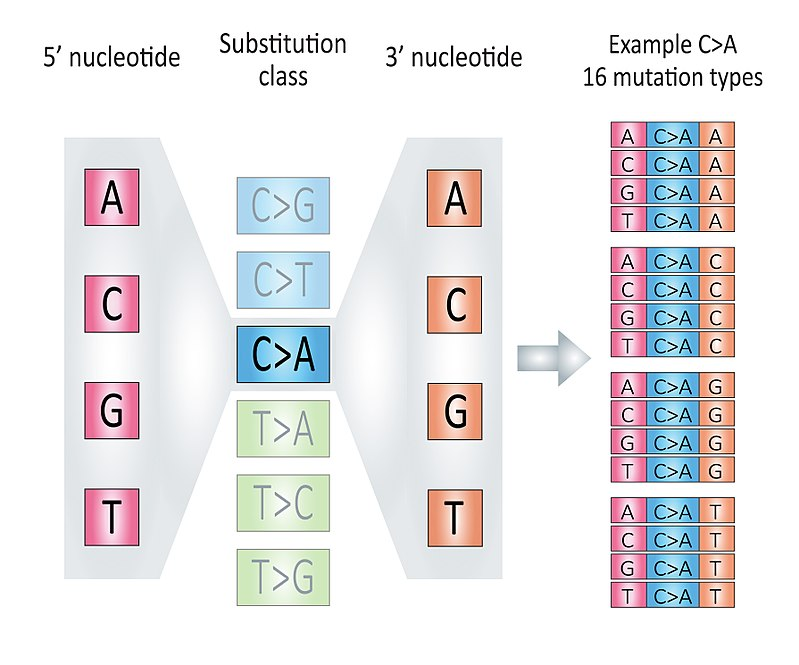
\includegraphics[width=0.95\linewidth]{fig/MutationTypes_v3} \caption{The illustration of 96 components, fig source: https://en.wikipedia.org/wiki/Mutational_signatures}\label{fig:unnamed-chunk-22}
\end{figure}

We tally components in each sample, and generate a sample-by-component matrix.

\begin{Shaded}
\begin{Highlighting}[]
\NormalTok{mt\_tally }\OtherTok{\textless{}{-}} \FunctionTok{sig\_tally}\NormalTok{(}
\NormalTok{  brca,}
  \AttributeTok{ref\_genome =} \StringTok{"BSgenome.Hsapiens.UCSC.hg19"}\NormalTok{,}
  \AttributeTok{use\_syn =} \ConstantTok{TRUE}
\NormalTok{)}
\DocumentationTok{\#\# i [2022{-}08{-}29 11:06:41]: Started.}
\DocumentationTok{\#\# i [2022{-}08{-}29 11:06:51]: We would assume you marked all variants\textquotesingle{} position in + strand.}
\DocumentationTok{\#\# }
\DocumentationTok{\#\# Attaching package: \textquotesingle{}S4Vectors\textquotesingle{}}
\DocumentationTok{\#\# The following objects are masked from \textquotesingle{}package:base\textquotesingle{}:}
\DocumentationTok{\#\# }
\DocumentationTok{\#\#     expand.grid, I, unname}
\DocumentationTok{\#\# }
\DocumentationTok{\#\# Attaching package: \textquotesingle{}Biostrings\textquotesingle{}}
\DocumentationTok{\#\# The following object is masked from \textquotesingle{}package:base\textquotesingle{}:}
\DocumentationTok{\#\# }
\DocumentationTok{\#\#     strsplit}
\DocumentationTok{\#\# v [2022{-}08{-}29 11:06:52]: Reference genome loaded.}
\DocumentationTok{\#\# v [2022{-}08{-}29 11:06:52]: Variants from MAF object queried.}
\DocumentationTok{\#\# v [2022{-}08{-}29 11:06:52]: Chromosome names checked.}
\DocumentationTok{\#\# v [2022{-}08{-}29 11:06:52]: Sex chromosomes properly handled.}
\DocumentationTok{\#\# v [2022{-}08{-}29 11:06:52]: Only variants located in standard chromosomes (1:22, X, Y, M/MT) are kept.}
\DocumentationTok{\#\# v [2022{-}08{-}29 11:06:52]: Variant start and end position checked.}
\DocumentationTok{\#\# v [2022{-}08{-}29 11:06:52]: Variant data for matrix generation preprocessed.}
\DocumentationTok{\#\# i [2022{-}08{-}29 11:06:52]: SBS matrix generation {-} start.}
\DocumentationTok{\#\# i [2022{-}08{-}29 11:06:52]: Extracting 5\textquotesingle{} and 3\textquotesingle{} adjacent bases.}
\DocumentationTok{\#\# i [2022{-}08{-}29 11:06:54]: Extracting +/{-} 20bp around mutated bases for background C\textgreater{}T estimation.}
\DocumentationTok{\#\# i [2022{-}08{-}29 11:06:55]: Estimating APOBEC enrichment scores.}
\DocumentationTok{\#\# i [2022{-}08{-}29 11:06:55]: Performing one{-}way Fisher\textquotesingle{}s test for APOBEC enrichment.}
\DocumentationTok{\#\# v [2022{-}08{-}29 11:06:55]: APOBEC related mutations are enriched in 28\% of samples (APOBEC enrichment score \textgreater{} 2; 28 of 100 samples)}
\DocumentationTok{\#\# i [2022{-}08{-}29 11:06:55]: Creating SBS sample{-}by{-}component matrices.}
\DocumentationTok{\#\# v [2022{-}08{-}29 11:06:55]: SBS{-}6 matrix created.}
\DocumentationTok{\#\# v [2022{-}08{-}29 11:06:55]: SBS{-}96 matrix created.}
\DocumentationTok{\#\# v [2022{-}08{-}29 11:06:55]: SBS{-}1536 matrix created.}
\DocumentationTok{\#\# i [2022{-}08{-}29 11:06:55]: Return SBS{-}96 as major matrix.}
\DocumentationTok{\#\# v [2022{-}08{-}29 11:06:55]: Done.}
\DocumentationTok{\#\# i [2022{-}08{-}29 11:06:55]: 13.577 secs elapsed.}
\end{Highlighting}
\end{Shaded}

\begin{quote}
Here set \texttt{use\_syn\ =\ TRUE} to include all variant records in MAF object to generate sample matrix.
\end{quote}

\begin{Shaded}
\begin{Highlighting}[]
\NormalTok{mt\_tally}\SpecialCharTok{$}\NormalTok{nmf\_matrix[}\DecValTok{1}\SpecialCharTok{:}\DecValTok{5}\NormalTok{, }\DecValTok{1}\SpecialCharTok{:}\DecValTok{5}\NormalTok{]}
\DocumentationTok{\#\#                              A[T\textgreater{}C]A C[T\textgreater{}C]A G[T\textgreater{}C]A T[T\textgreater{}C]A A[C\textgreater{}T]A}
\DocumentationTok{\#\# TCGA{-}A1{-}A0SH{-}01A{-}11D{-}A099{-}09       0       0       1       1       0}
\DocumentationTok{\#\# TCGA{-}A2{-}A04N{-}01A{-}11D{-}A10Y{-}09       0       0       0       1       2}
\DocumentationTok{\#\# TCGA{-}A2{-}A0CP{-}01A{-}11W{-}A050{-}09       0       0       0       0       0}
\DocumentationTok{\#\# TCGA{-}A2{-}A0EP{-}01A{-}52D{-}A22X{-}09       0       0       1       0       0}
\DocumentationTok{\#\# TCGA{-}A2{-}A0EV{-}01A{-}11W{-}A050{-}09       0       0       1       0       0}
\end{Highlighting}
\end{Shaded}

We use notion \texttt{left{[}ref\textgreater{}mut{]}right} to mark each component, e.g.~\texttt{C{[}T\textgreater{}G{]}A} means a base T with 5' adjacent base C and 3' adjacent base A is mutated to base G.

\hypertarget{other-situations}{%
\subsection{Other Situations}\label{other-situations}}

Above we show the most common SBS classifications, there are other situations supported by \textbf{sigminer}, including other classifications for SBS records and other mutation types (DBS and ID). All situations about SBS, DBS and ID signatures are well documented in \href{https://osf.io/s93d5/wiki/home/}{wiki of \textbf{SigProfilerMatrixGenerator} package}.

\hypertarget{other-sbs-classifications}{%
\subsubsection{Other SBS classifications}\label{other-sbs-classifications}}

After calling \texttt{sig\_tally()}, the most used matrix is stored in \texttt{nmf\_matrix}, and all matrices generated by \textbf{sigminer} are stored in \texttt{all\_matrices}.

\begin{Shaded}
\begin{Highlighting}[]
\FunctionTok{str}\NormalTok{(mt\_tally}\SpecialCharTok{$}\NormalTok{all\_matrices, }\AttributeTok{max.level =} \DecValTok{1}\NormalTok{)}
\DocumentationTok{\#\# List of 3}
\DocumentationTok{\#\#  $ SBS\_6   : int [1:100, 1:6] 7 6 5 4 9 7 5 5 0 5 ...}
\DocumentationTok{\#\#   ..{-} attr(*, "dimnames")=List of 2}
\DocumentationTok{\#\#  $ SBS\_96  : int [1:100, 1:96] 0 0 0 0 0 0 1 2 0 0 ...}
\DocumentationTok{\#\#   ..{-} attr(*, "dimnames")=List of 2}
\DocumentationTok{\#\#  $ SBS\_1536: int [1:100, 1:1536] 0 0 0 0 0 0 0 0 0 0 ...}
\DocumentationTok{\#\#   ..{-} attr(*, "dimnames")=List of 2}
\end{Highlighting}
\end{Shaded}

If you add the strand classification, all matrices can be generated by \textbf{sigminer} will return.

\begin{Shaded}
\begin{Highlighting}[]
\NormalTok{mt\_tally2 }\OtherTok{\textless{}{-}} \FunctionTok{sig\_tally}\NormalTok{(}
\NormalTok{  brca,}
  \AttributeTok{ref\_genome =} \StringTok{"BSgenome.Hsapiens.UCSC.hg19"}\NormalTok{,}
  \AttributeTok{use\_syn =} \ConstantTok{TRUE}\NormalTok{, }\AttributeTok{add\_trans\_bias =} \ConstantTok{TRUE}
\NormalTok{)}
\DocumentationTok{\#\# i [2022{-}08{-}29 11:06:56]: Started.}
\DocumentationTok{\#\# i [2022{-}08{-}29 11:06:56]: We would assume you marked all variants\textquotesingle{} position in + strand.}
\DocumentationTok{\#\# v [2022{-}08{-}29 11:06:56]: Reference genome loaded.}
\DocumentationTok{\#\# v [2022{-}08{-}29 11:06:56]: Variants from MAF object queried.}
\DocumentationTok{\#\# v [2022{-}08{-}29 11:06:56]: Chromosome names checked.}
\DocumentationTok{\#\# v [2022{-}08{-}29 11:06:56]: Sex chromosomes properly handled.}
\DocumentationTok{\#\# v [2022{-}08{-}29 11:06:56]: Only variants located in standard chromosomes (1:22, X, Y, M/MT) are kept.}
\DocumentationTok{\#\# v [2022{-}08{-}29 11:06:56]: Variant start and end position checked.}
\DocumentationTok{\#\# v [2022{-}08{-}29 11:06:56]: Variant data for matrix generation preprocessed.}
\DocumentationTok{\#\# i [2022{-}08{-}29 11:06:56]: SBS matrix generation {-} start.}
\DocumentationTok{\#\# i [2022{-}08{-}29 11:06:56]: Extracting 5\textquotesingle{} and 3\textquotesingle{} adjacent bases.}
\DocumentationTok{\#\# i [2022{-}08{-}29 11:06:56]: Extracting +/{-} 20bp around mutated bases for background C\textgreater{}T estimation.}
\DocumentationTok{\#\# i [2022{-}08{-}29 11:06:57]: Estimating APOBEC enrichment scores.}
\DocumentationTok{\#\# i [2022{-}08{-}29 11:06:57]: Performing one{-}way Fisher\textquotesingle{}s test for APOBEC enrichment.}
\DocumentationTok{\#\# v [2022{-}08{-}29 11:06:57]: APOBEC related mutations are enriched in 28\% of samples (APOBEC enrichment score \textgreater{} 2; 28 of 100 samples)}
\DocumentationTok{\#\# i [2022{-}08{-}29 11:06:57]: Creating SBS sample{-}by{-}component matrices.}
\DocumentationTok{\#\# v [2022{-}08{-}29 11:06:57]: SBS{-}6 matrix created.}
\DocumentationTok{\#\# v [2022{-}08{-}29 11:06:57]: SBS{-}96 matrix created.}
\DocumentationTok{\#\# v [2022{-}08{-}29 11:06:57]: SBS{-}1536 matrix created.}
\DocumentationTok{\#\# v [2022{-}08{-}29 11:06:58]: SBS{-}24 (6x4) matrix created.}
\DocumentationTok{\#\# v [2022{-}08{-}29 11:06:58]: SBS{-}384 (96x4) matrix created.}
\DocumentationTok{\#\# v [2022{-}08{-}29 11:06:59]: SBS{-}6144 (1536x4) matrix created.}
\DocumentationTok{\#\# i [2022{-}08{-}29 11:06:59]: Return SBS{-}192 as major matrix.}
\DocumentationTok{\#\# v [2022{-}08{-}29 11:06:59]: Done.}
\DocumentationTok{\#\# i [2022{-}08{-}29 11:06:59]: 3.079 secs elapsed.}
\FunctionTok{str}\NormalTok{(mt\_tally2}\SpecialCharTok{$}\NormalTok{all\_matrices, }\AttributeTok{max.level =} \DecValTok{1}\NormalTok{)}
\DocumentationTok{\#\# List of 7}
\DocumentationTok{\#\#  $ SBS\_6   : int [1:100, 1:6] 7 6 5 4 9 7 5 5 0 5 ...}
\DocumentationTok{\#\#   ..{-} attr(*, "dimnames")=List of 2}
\DocumentationTok{\#\#  $ SBS\_24  : int [1:100, 1:24] 6 3 3 2 6 4 1 2 0 3 ...}
\DocumentationTok{\#\#   ..{-} attr(*, "dimnames")=List of 2}
\DocumentationTok{\#\#  $ SBS\_96  : int [1:100, 1:96] 0 0 0 0 0 0 1 2 0 0 ...}
\DocumentationTok{\#\#   ..{-} attr(*, "dimnames")=List of 2}
\DocumentationTok{\#\#  $ SBS\_192 : int [1:100, 1:192] 0 0 0 0 0 0 0 0 0 0 ...}
\DocumentationTok{\#\#   ..{-} attr(*, "dimnames")=List of 2}
\DocumentationTok{\#\#  $ SBS\_384 : int [1:100, 1:384] 0 0 0 0 0 0 0 0 0 0 ...}
\DocumentationTok{\#\#   ..{-} attr(*, "dimnames")=List of 2}
\DocumentationTok{\#\#  $ SBS\_1536: int [1:100, 1:1536] 0 0 0 0 0 0 0 0 0 0 ...}
\DocumentationTok{\#\#   ..{-} attr(*, "dimnames")=List of 2}
\DocumentationTok{\#\#  $ SBS\_6144: int [1:100, 1:6144] 0 0 0 0 0 0 0 0 0 0 ...}
\DocumentationTok{\#\#   ..{-} attr(*, "dimnames")=List of 2}
\end{Highlighting}
\end{Shaded}

\hypertarget{dbs-and-id-components}{%
\subsubsection{DBS and ID components}\label{dbs-and-id-components}}

If you want to generate DBS or ID matrices, just modify the \texttt{mode} option.

\begin{Shaded}
\begin{Highlighting}[]
\NormalTok{mt\_tally\_DBS }\OtherTok{\textless{}{-}} \FunctionTok{sig\_tally}\NormalTok{(}
\NormalTok{  brca,}
  \AttributeTok{ref\_genome =} \StringTok{"BSgenome.Hsapiens.UCSC.hg19"}\NormalTok{,}
  \AttributeTok{use\_syn =} \ConstantTok{TRUE}\NormalTok{,}
  \AttributeTok{mode =} \StringTok{"DBS"}\NormalTok{,}
  \AttributeTok{add\_trans\_bias =} \ConstantTok{TRUE}
\NormalTok{)}
\DocumentationTok{\#\# i [2022{-}08{-}29 11:06:59]: Started.}
\DocumentationTok{\#\# i [2022{-}08{-}29 11:06:59]: We would assume you marked all variants\textquotesingle{} position in + strand.}
\DocumentationTok{\#\# v [2022{-}08{-}29 11:06:59]: Reference genome loaded.}
\DocumentationTok{\#\# v [2022{-}08{-}29 11:06:59]: Variants from MAF object queried.}
\DocumentationTok{\#\# v [2022{-}08{-}29 11:06:59]: Chromosome names checked.}
\DocumentationTok{\#\# v [2022{-}08{-}29 11:06:59]: Sex chromosomes properly handled.}
\DocumentationTok{\#\# v [2022{-}08{-}29 11:06:59]: Only variants located in standard chromosomes (1:22, X, Y, M/MT) are kept.}
\DocumentationTok{\#\# v [2022{-}08{-}29 11:06:59]: Variant start and end position checked.}
\DocumentationTok{\#\# v [2022{-}08{-}29 11:06:59]: Variant data for matrix generation preprocessed.}
\DocumentationTok{\#\# i [2022{-}08{-}29 11:06:59]: DBS matrix generation {-} start.}
\DocumentationTok{\#\# i [2022{-}08{-}29 11:06:59]: Searching DBS records...}
\DocumentationTok{\#\# v [2022{-}08{-}29 11:07:00]: Done.}
\DocumentationTok{\#\# v [2022{-}08{-}29 11:07:02]: Reference sequences queried from genome.}
\DocumentationTok{\#\# v [2022{-}08{-}29 11:07:02]: DBS{-}78 matrix created.}
\DocumentationTok{\#\# v [2022{-}08{-}29 11:07:02]: DBS{-}1248 matrix created.}
\DocumentationTok{\#\# v [2022{-}08{-}29 11:07:02]: DBS{-}186 matrix created.}
\DocumentationTok{\#\# i [2022{-}08{-}29 11:07:02]: Return DBS{-}186 as major matrix.}
\DocumentationTok{\#\# v [2022{-}08{-}29 11:07:02]: Done.}
\DocumentationTok{\#\# i [2022{-}08{-}29 11:07:02]: 2.59 secs elapsed.}
\FunctionTok{str}\NormalTok{(mt\_tally\_DBS}\SpecialCharTok{$}\NormalTok{all\_matrices, }\AttributeTok{max.level =} \DecValTok{1}\NormalTok{)}
\DocumentationTok{\#\# List of 3}
\DocumentationTok{\#\#  $ DBS\_78  : int [1:100, 1:78] 0 0 0 0 0 0 0 0 0 0 ...}
\DocumentationTok{\#\#   ..{-} attr(*, "dimnames")=List of 2}
\DocumentationTok{\#\#  $ DBS\_186 : int [1:100, 1:186] 0 0 0 0 0 0 0 0 0 0 ...}
\DocumentationTok{\#\#   ..{-} attr(*, "dimnames")=List of 2}
\DocumentationTok{\#\#  $ DBS\_1248: int [1:100, 1:1248] 0 0 0 0 0 0 0 0 0 0 ...}
\DocumentationTok{\#\#   ..{-} attr(*, "dimnames")=List of 2}
\end{Highlighting}
\end{Shaded}

\begin{quote}
Program will stop if no records to analyze.
Let's see ID records.
\end{quote}

\begin{Shaded}
\begin{Highlighting}[]
\NormalTok{mt\_tally\_ID }\OtherTok{\textless{}{-}} \FunctionTok{sig\_tally}\NormalTok{(}
\NormalTok{  brca,}
  \AttributeTok{ref\_genome =} \StringTok{"BSgenome.Hsapiens.UCSC.hg19"}\NormalTok{,}
  \AttributeTok{use\_syn =} \ConstantTok{TRUE}\NormalTok{,}
  \AttributeTok{mode =} \StringTok{"ID"}\NormalTok{,}
  \AttributeTok{add\_trans\_bias =} \ConstantTok{TRUE}
\NormalTok{)}
\DocumentationTok{\#\# i [2022{-}08{-}29 11:07:02]: Started.}
\DocumentationTok{\#\# i [2022{-}08{-}29 11:07:02]: We would assume you marked all variants\textquotesingle{} position in + strand.}
\DocumentationTok{\#\# v [2022{-}08{-}29 11:07:02]: Reference genome loaded.}
\DocumentationTok{\#\# v [2022{-}08{-}29 11:07:02]: Variants from MAF object queried.}
\DocumentationTok{\#\# v [2022{-}08{-}29 11:07:02]: Chromosome names checked.}
\DocumentationTok{\#\# v [2022{-}08{-}29 11:07:02]: Sex chromosomes properly handled.}
\DocumentationTok{\#\# v [2022{-}08{-}29 11:07:02]: Only variants located in standard chromosomes (1:22, X, Y, M/MT) are kept.}
\DocumentationTok{\#\# v [2022{-}08{-}29 11:07:02]: Variant start and end position checked.}
\DocumentationTok{\#\# v [2022{-}08{-}29 11:07:02]: Variant data for matrix generation preprocessed.}
\DocumentationTok{\#\# i [2022{-}08{-}29 11:07:02]: INDEL matrix generation {-} start.}
\DocumentationTok{\#\# v [2022{-}08{-}29 11:07:05]: Reference sequences queried from genome.}
\DocumentationTok{\#\# v [2022{-}08{-}29 11:07:05]: INDEL length extracted.}
\DocumentationTok{\#\# v [2022{-}08{-}29 11:07:05]: Adjacent copies counted.}
\DocumentationTok{\#\# v [2022{-}08{-}29 11:07:33]: Microhomology size calculated.}
\DocumentationTok{\#\# v [2022{-}08{-}29 11:07:33]: INDEL records classified into different components (types).}
\DocumentationTok{\#\# v [2022{-}08{-}29 11:07:33]: ID{-}28 matrix created.}
\DocumentationTok{\#\# v [2022{-}08{-}29 11:07:33]: ID{-}83 matrix created.}
\DocumentationTok{\#\# v [2022{-}08{-}29 11:07:33]: ID{-}415 matrix created.}
\DocumentationTok{\#\# i [2022{-}08{-}29 11:07:33]: Return ID{-}415 as major matrix.}
\DocumentationTok{\#\# v [2022{-}08{-}29 11:07:33]: Done.}
\DocumentationTok{\#\# i [2022{-}08{-}29 11:07:33]: 30.713 secs elapsed.}
\FunctionTok{str}\NormalTok{(mt\_tally\_ID}\SpecialCharTok{$}\NormalTok{all\_matrices, }\AttributeTok{max.level =} \DecValTok{1}\NormalTok{)}
\DocumentationTok{\#\# List of 3}
\DocumentationTok{\#\#  $ ID\_28 : int [1:100, 1:28] 0 1 0 0 0 0 0 0 0 0 ...}
\DocumentationTok{\#\#   ..{-} attr(*, "dimnames")=List of 2}
\DocumentationTok{\#\#  $ ID\_83 : int [1:100, 1:83] 0 1 0 0 0 0 0 0 0 0 ...}
\DocumentationTok{\#\#   ..{-} attr(*, "dimnames")=List of 2}
\DocumentationTok{\#\#  $ ID\_415:\textquotesingle{}data.frame\textquotesingle{}:  100 obs. of  415 variables:}
\end{Highlighting}
\end{Shaded}

\hypertarget{take-togother}{%
\subsubsection{Take togother}\label{take-togother}}

If you want to get all matrices for SBS, DBS and ID at the same time, you don't need to write a \texttt{for} loop or type three times to do this.
Just set \texttt{mode=\textquotesingle{}ALL\textquotesingle{}}, \textbf{sigminer} will do it for you!

\begin{Shaded}
\begin{Highlighting}[]
\NormalTok{mt\_tally\_all }\OtherTok{\textless{}{-}} \FunctionTok{sig\_tally}\NormalTok{(}
\NormalTok{  brca,}
  \AttributeTok{ref\_genome =} \StringTok{"BSgenome.Hsapiens.UCSC.hg19"}\NormalTok{,}
  \AttributeTok{use\_syn =} \ConstantTok{TRUE}\NormalTok{,}
  \AttributeTok{mode =} \StringTok{"ALL"}\NormalTok{,}
  \AttributeTok{add\_trans\_bias =} \ConstantTok{TRUE}
\NormalTok{)}
\DocumentationTok{\#\# i [2022{-}08{-}29 11:07:33]: Started.}
\DocumentationTok{\#\# i [2022{-}08{-}29 11:07:33]: We would assume you marked all variants\textquotesingle{} position in + strand.}
\DocumentationTok{\#\# v [2022{-}08{-}29 11:07:33]: Reference genome loaded.}
\DocumentationTok{\#\# v [2022{-}08{-}29 11:07:33]: Variants from MAF object queried.}
\DocumentationTok{\#\# v [2022{-}08{-}29 11:07:33]: Chromosome names checked.}
\DocumentationTok{\#\# v [2022{-}08{-}29 11:07:33]: Sex chromosomes properly handled.}
\DocumentationTok{\#\# v [2022{-}08{-}29 11:07:33]: Only variants located in standard chromosomes (1:22, X, Y, M/MT) are kept.}
\DocumentationTok{\#\# v [2022{-}08{-}29 11:07:33]: Variant start and end position checked.}
\DocumentationTok{\#\# v [2022{-}08{-}29 11:07:33]: Variant data for matrix generation preprocessed.}
\DocumentationTok{\#\# i [2022{-}08{-}29 11:07:33]: All types of matrices generation {-} start.}
\DocumentationTok{\#\# i [2022{-}08{-}29 11:07:33]: SBS matrix generation {-} start.}
\DocumentationTok{\#\# i [2022{-}08{-}29 11:07:33]: Extracting 5\textquotesingle{} and 3\textquotesingle{} adjacent bases.}
\DocumentationTok{\#\# i [2022{-}08{-}29 11:07:34]: Extracting +/{-} 20bp around mutated bases for background C\textgreater{}T estimation.}
\DocumentationTok{\#\# i [2022{-}08{-}29 11:07:35]: Estimating APOBEC enrichment scores.}
\DocumentationTok{\#\# i [2022{-}08{-}29 11:07:35]: Performing one{-}way Fisher\textquotesingle{}s test for APOBEC enrichment.}
\DocumentationTok{\#\# v [2022{-}08{-}29 11:07:35]: APOBEC related mutations are enriched in 28\% of samples (APOBEC enrichment score \textgreater{} 2; 28 of 100 samples)}
\DocumentationTok{\#\# i [2022{-}08{-}29 11:07:35]: Creating SBS sample{-}by{-}component matrices.}
\DocumentationTok{\#\# v [2022{-}08{-}29 11:07:35]: SBS{-}6 matrix created.}
\DocumentationTok{\#\# v [2022{-}08{-}29 11:07:35]: SBS{-}96 matrix created.}
\DocumentationTok{\#\# v [2022{-}08{-}29 11:07:35]: SBS{-}1536 matrix created.}
\DocumentationTok{\#\# v [2022{-}08{-}29 11:07:35]: SBS{-}24 (6x4) matrix created.}
\DocumentationTok{\#\# v [2022{-}08{-}29 11:07:35]: SBS{-}384 (96x4) matrix created.}
\DocumentationTok{\#\# v [2022{-}08{-}29 11:07:36]: SBS{-}6144 (1536x4) matrix created.}
\DocumentationTok{\#\# i [2022{-}08{-}29 11:07:36]: Return SBS{-}192 as major matrix.}
\DocumentationTok{\#\# i [2022{-}08{-}29 11:07:36]: DBS matrix generation {-} start.}
\DocumentationTok{\#\# i [2022{-}08{-}29 11:07:36]: Searching DBS records...}
\DocumentationTok{\#\# v [2022{-}08{-}29 11:07:37]: Done.}
\DocumentationTok{\#\# v [2022{-}08{-}29 11:07:38]: Reference sequences queried from genome.}
\DocumentationTok{\#\# v [2022{-}08{-}29 11:07:38]: DBS{-}78 matrix created.}
\DocumentationTok{\#\# v [2022{-}08{-}29 11:07:38]: DBS{-}1248 matrix created.}
\DocumentationTok{\#\# v [2022{-}08{-}29 11:07:38]: DBS{-}186 matrix created.}
\DocumentationTok{\#\# i [2022{-}08{-}29 11:07:38]: Return DBS{-}186 as major matrix.}
\DocumentationTok{\#\# i [2022{-}08{-}29 11:07:38]: INDEL matrix generation {-} start.}
\DocumentationTok{\#\# v [2022{-}08{-}29 11:07:40]: Reference sequences queried from genome.}
\DocumentationTok{\#\# v [2022{-}08{-}29 11:07:40]: INDEL length extracted.}
\DocumentationTok{\#\# v [2022{-}08{-}29 11:07:40]: Adjacent copies counted.}
\DocumentationTok{\#\# v [2022{-}08{-}29 11:08:08]: Microhomology size calculated.}
\DocumentationTok{\#\# v [2022{-}08{-}29 11:08:08]: INDEL records classified into different components (types).}
\DocumentationTok{\#\# v [2022{-}08{-}29 11:08:08]: ID{-}28 matrix created.}
\DocumentationTok{\#\# v [2022{-}08{-}29 11:08:08]: ID{-}83 matrix created.}
\DocumentationTok{\#\# v [2022{-}08{-}29 11:08:08]: ID{-}415 matrix created.}
\DocumentationTok{\#\# i [2022{-}08{-}29 11:08:08]: Return ID{-}415 as major matrix.}
\DocumentationTok{\#\# i [2022{-}08{-}29 11:08:08]: All types of matrices generation (APOBEC scores included) {-} end.}
\DocumentationTok{\#\# v [2022{-}08{-}29 11:08:08]: Done.}
\DocumentationTok{\#\# i [2022{-}08{-}29 11:08:08]: 35.388 secs elapsed.}
\FunctionTok{str}\NormalTok{(mt\_tally\_all, }\AttributeTok{max.level =} \DecValTok{1}\NormalTok{)}
\DocumentationTok{\#\# List of 14}
\DocumentationTok{\#\#  $ SBS\_6        : int [1:100, 1:6] 7 6 5 4 9 7 5 5 0 5 ...}
\DocumentationTok{\#\#   ..{-} attr(*, "dimnames")=List of 2}
\DocumentationTok{\#\#  $ SBS\_24       : int [1:100, 1:24] 6 3 3 2 6 4 1 2 0 3 ...}
\DocumentationTok{\#\#   ..{-} attr(*, "dimnames")=List of 2}
\DocumentationTok{\#\#  $ SBS\_96       : int [1:100, 1:96] 0 0 0 0 0 0 1 2 0 0 ...}
\DocumentationTok{\#\#   ..{-} attr(*, "dimnames")=List of 2}
\DocumentationTok{\#\#  $ SBS\_192      : int [1:100, 1:192] 0 0 0 0 0 0 0 0 0 0 ...}
\DocumentationTok{\#\#   ..{-} attr(*, "dimnames")=List of 2}
\DocumentationTok{\#\#  $ SBS\_384      : int [1:100, 1:384] 0 0 0 0 0 0 0 0 0 0 ...}
\DocumentationTok{\#\#   ..{-} attr(*, "dimnames")=List of 2}
\DocumentationTok{\#\#  $ SBS\_1536     : int [1:100, 1:1536] 0 0 0 0 0 0 0 0 0 0 ...}
\DocumentationTok{\#\#   ..{-} attr(*, "dimnames")=List of 2}
\DocumentationTok{\#\#  $ SBS\_6144     : int [1:100, 1:6144] 0 0 0 0 0 0 0 0 0 0 ...}
\DocumentationTok{\#\#   ..{-} attr(*, "dimnames")=List of 2}
\DocumentationTok{\#\#  $ DBS\_78       : int [1:100, 1:78] 0 0 0 0 0 0 0 0 0 0 ...}
\DocumentationTok{\#\#   ..{-} attr(*, "dimnames")=List of 2}
\DocumentationTok{\#\#  $ DBS\_186      : int [1:100, 1:186] 0 0 0 0 0 0 0 0 0 0 ...}
\DocumentationTok{\#\#   ..{-} attr(*, "dimnames")=List of 2}
\DocumentationTok{\#\#  $ DBS\_1248     : int [1:100, 1:1248] 0 0 0 0 0 0 0 0 0 0 ...}
\DocumentationTok{\#\#   ..{-} attr(*, "dimnames")=List of 2}
\DocumentationTok{\#\#  $ ID\_28        : int [1:100, 1:28] 0 1 0 0 0 0 0 0 0 0 ...}
\DocumentationTok{\#\#   ..{-} attr(*, "dimnames")=List of 2}
\DocumentationTok{\#\#  $ ID\_83        : int [1:100, 1:83] 0 1 0 0 0 0 0 0 0 0 ...}
\DocumentationTok{\#\#   ..{-} attr(*, "dimnames")=List of 2}
\DocumentationTok{\#\#  $ ID\_415       :\textquotesingle{}data.frame\textquotesingle{}:   100 obs. of  415 variables:}
\DocumentationTok{\#\#  $ APOBEC\_scores:Classes \textquotesingle{}data.table\textquotesingle{} and \textquotesingle{}data.frame\textquotesingle{}:  100 obs. of  44 variables:}
\DocumentationTok{\#\#   ..{-} attr(*, ".internal.selfref")=\textless{}externalptr\textgreater{} }
\DocumentationTok{\#\#   ..{-} attr(*, "index")= int(0) }
\DocumentationTok{\#\#   .. ..{-} attr(*, "\_\_APOBEC\_Enriched")= int [1:100] 17 21 23 24 25 26 27 28 30 32 ...}
\end{Highlighting}
\end{Shaded}

Please note, in this case, just a list containing matrices will return.

\hypertarget{de-novo-signature-discovery}{%
\section{\texorpdfstring{\emph{de novo} signature discovery}{de novo signature discovery}}\label{de-novo-signature-discovery}}

\textbf{Sigminer} provides many approaches to extract mutational signatures. To test their performances, We use 4 mutation catalog datasets (each mutation catalog dataset is composed of 30 samples, 10 COSMIC v2 (SBS) signatures are randomly assigned to each sample with random signature exposure/activity) from \citet{degasperi2020practical}. The following table shows how many signatures can be recovered and the corresponding average cosine similarity to COSMIC reference signatures for each approach with settings.

\begin{longtable}[]{@{}
  >{\raggedright\arraybackslash}p{(\columnwidth - 24\tabcolsep) * \real{0.0372}}
  >{\raggedright\arraybackslash}p{(\columnwidth - 24\tabcolsep) * \real{0.0546}}
  >{\raggedright\arraybackslash}p{(\columnwidth - 24\tabcolsep) * \real{0.1365}}
  >{\raggedright\arraybackslash}p{(\columnwidth - 24\tabcolsep) * \real{0.0769}}
  >{\raggedright\arraybackslash}p{(\columnwidth - 24\tabcolsep) * \real{0.0273}}
  >{\raggedright\arraybackslash}p{(\columnwidth - 24\tabcolsep) * \real{0.0422}}
  >{\raggedright\arraybackslash}p{(\columnwidth - 24\tabcolsep) * \real{0.0298}}
  >{\raggedright\arraybackslash}p{(\columnwidth - 24\tabcolsep) * \real{0.0298}}
  >{\raggedright\arraybackslash}p{(\columnwidth - 24\tabcolsep) * \real{0.0422}}
  >{\raggedright\arraybackslash}p{(\columnwidth - 24\tabcolsep) * \real{0.0298}}
  >{\raggedright\arraybackslash}p{(\columnwidth - 24\tabcolsep) * \real{0.0372}}
  >{\raggedright\arraybackslash}p{(\columnwidth - 24\tabcolsep) * \real{0.0471}}
  >{\raggedright\arraybackslash}p{(\columnwidth - 24\tabcolsep) * \real{0.4094}}@{}}
\toprule()
\begin{minipage}[b]{\linewidth}\raggedright
Approach
\end{minipage} & \begin{minipage}[b]{\linewidth}\raggedright
Selection Way
\end{minipage} & \begin{minipage}[b]{\linewidth}\raggedright
Setting
\end{minipage} & \begin{minipage}[b]{\linewidth}\raggedright
Caller
\end{minipage} & \begin{minipage}[b]{\linewidth}\raggedright
Recommend
\end{minipage} & \begin{minipage}[b]{\linewidth}\raggedright
Driver
\end{minipage} & \begin{minipage}[b]{\linewidth}\raggedright
Set1
\end{minipage} & \begin{minipage}[b]{\linewidth}\raggedright
Set2
\end{minipage} & \begin{minipage}[b]{\linewidth}\raggedright
Set3
\end{minipage} & \begin{minipage}[b]{\linewidth}\raggedright
Set4
\end{minipage} & \begin{minipage}[b]{\linewidth}\raggedright
Success /Mean
\end{minipage} & \begin{minipage}[b]{\linewidth}\raggedright
Run time
\end{minipage} & \begin{minipage}[b]{\linewidth}\raggedright
Note
\end{minipage} \\
\midrule()
\endhead
Standard NMF & Manual & Default. 50 runs (estimation) + 100 runs (extraction) & \texttt{sig\_estimate}, \texttt{sig\_extract} & YES ⭐⭐⭐ & R & 10 (0.884) & 10 (0.944) & 9 or 10 (0.998) & 10 (0.994) & \textasciitilde90\%/0.955 & \textasciitilde1min (8 cores) & This is a basic method, suitable for good mutation data with enough mutations. \\
SigProfiler & \textbf{Manual/Automatic} & Default. 100 runs & \texttt{sigprofiler\_extract} & YES ⭐⭐⭐⭐ & Python/Anaconda & 10 (0.961) & 10 (0.999) & 10 (0.990) & 10 (0.997) & 100\%/0.987 & \textasciitilde1h (8 cores) & A golden standard like approach in this field, but longer run time, and the requirement for Python environment and extra large packages reduce its popularity here. \\
Best Practice & \textbf{Manual/Automatic} & Use bootstrapped catalog (1000 runs) & \texttt{bp\_extract\_signatures} & YES ⭐⭐⭐⭐⭐ & R & 10 (0.973) & 10 (0.990) & 10 (0.992) & 10 (0.971) & 100\%/0.981 & \textasciitilde10min (8 cores) & My R implementation for methods from reference \#5 and \#6. Should be the best option here. (\textbf{Pay attention to the suggested solution}) \\
Best Practice & \textbf{Manual/Automatic} & Use original catalog (1000 runs) & \texttt{bp\_extract\_signatures} & NO :star: & R & 10 (0.987) & 9 (0.985) & 10 (0.997) & 9 (0.987) & 50\%/0.989 & \textasciitilde10min (8 cores) & This is created to compare with the approach with bootstrapped catalogs above and the standard NMF way. \\
Bayesian NMF & \textbf{Automatic} & L1KL+optimal (20 runs) & \texttt{sig\_auto\_extract} & YES ⭐⭐⭐ & R & 10 (0.994) & 9 (0.997) & 9 (0.998) & 9 (0.999) & 25\%/0.997 & \textasciitilde10min (8 cores) & The Bayesian NMF approach auto reduce the signature number to a proper value from a initial signature number, here is 20. \\
Bayesian NMF & \textbf{Automatic} & L1KL+stable (20 runs) & \texttt{sig\_auto\_extract} & YES ⭐⭐⭐⭐ & R & 10 (0.994) & 9 (0.997) & 10 (0.988) & 9 (0.999) & 50\%/0.995 & \textasciitilde10min (8 cores) & See above. \\
Bayesian NMF & \textbf{Automatic} & L2KL+optimal (20 runs) & \texttt{sig\_auto\_extract} & NO :star: & R & 12 (0.990) & 13 (0.988) & 12 (0.902) & 12 (0.994) & 0\%/0.969 & \textasciitilde10min (8 cores) & See above. \\
Bayesian NMF & \textbf{Automatic} & L2KL+stable (20 runs) & \texttt{sig\_auto\_extract} & NO :star: & R & 12 (0.990) & 12 (0.988) & 12 (0.902) & 12 (0.994) & 0\%/0.969 & \textasciitilde10min (8 cores) & See above. \\
Bayesian NMF & \textbf{Automatic} & L1WL2H+optimal (20 runs) & \texttt{sig\_auto\_extract} & YES ⭐⭐⭐ & R & 9 (0.989) & 9 (0.999) & 9 (0.996) & 9 (1.000) & 0\%/0.996 & \textasciitilde10min (8 cores) & See above. \\
Bayesian NMF & \textbf{Automatic} & L1WL2H+stable (20 runs) & \texttt{sig\_auto\_extract} & YES ⭐⭐⭐⭐ & R & 9 (0.989) & 9 (0.999) & 9 (0.996) & 9 (1.000) & 0\%/0.996 & \textasciitilde10min (8 cores) & See above. \\
\bottomrule()
\end{longtable}

\begin{quote}
NOTE: although Bayesian NMF approach with L1KL or L1WL2H prior cannot recover all 10 signatures here, but it is close to the true answer from initial signature number 20 in a automatic way, and the result signatures are highly similar to reference signatures. This also reminds us that we could not use this method to find signatures with small contributions in tumors.
\end{quote}

From \textbf{sigminer} v2.1.0, an unified interface \texttt{sig\_unify\_extract()}. has been implemented to access the
4 signature extraction approaches.

\begin{Shaded}
\begin{Highlighting}[]
\FunctionTok{args}\NormalTok{(sig\_unify\_extract)}
\DocumentationTok{\#\# function (nmf\_matrix, range = 2:5, nrun = 10, approach = c("bayes\_nmf", }
\DocumentationTok{\#\#     "repeated\_nmf", "bootstrap\_nmf", "sigprofiler"), cores = 1L, }
\DocumentationTok{\#\#     ...) }
\DocumentationTok{\#\# NULL}
\end{Highlighting}
\end{Shaded}

Once you determine a method, please read all parameters shown in the detail function.

\begin{itemize}
\tightlist
\item
  ``bayes\_nmf'' corresponds to \texttt{sig\_auto\_extract()}.
\item
  ``repeated\_nmf'' corresponds to \texttt{sig\_extract()}.
\item
  ``bootstrap\_nmf'' coresponds to \texttt{bp\_extract\_signatures()}.
\item
  ``sigprofiler'' corresponds to \texttt{sigprofiler\_extract()}.
\end{itemize}

Note, when you use \texttt{sig\_extract()} (``repeated\_nmf'') and you don't know how
to select the signature number, you should run \texttt{sig\_estimate()} firstly.

\hypertarget{manual-signature-estimation-and-extraction}{%
\subsection{Manual signature estimation and extraction}\label{manual-signature-estimation-and-extraction}}

For example, let's try signature number 2-6. For simplicity, we just run NMF 10 times for each signature number. We use 4 cores to speed up the computation.

\begin{Shaded}
\begin{Highlighting}[]
\NormalTok{mt\_est }\OtherTok{\textless{}{-}} \FunctionTok{sig\_estimate}\NormalTok{(mt\_tally}\SpecialCharTok{$}\NormalTok{nmf\_matrix,}
  \AttributeTok{range =} \DecValTok{2}\SpecialCharTok{:}\DecValTok{6}\NormalTok{,}
  \AttributeTok{nrun =} \DecValTok{10}\NormalTok{, }\CommentTok{\# increase this value if you wana a more stable estimation}
  \AttributeTok{use\_random =} \ConstantTok{FALSE}\NormalTok{, }\CommentTok{\# if TRUE, add results from randomized input}
  \AttributeTok{cores =} \DecValTok{4}\NormalTok{,}
  \AttributeTok{verbose =} \ConstantTok{TRUE}
\NormalTok{)}
\end{Highlighting}
\end{Shaded}

We can show signature number survey for different measures by \texttt{show\_sig\_number\_survey2()}.

\begin{Shaded}
\begin{Highlighting}[]
\DocumentationTok{\#\# You can also select the measures to show}
\DocumentationTok{\#\# by \textquotesingle{}what\textquotesingle{} option}
\FunctionTok{show\_sig\_number\_survey2}\NormalTok{(mt\_est}\SpecialCharTok{$}\NormalTok{survey)}
\end{Highlighting}
\end{Shaded}

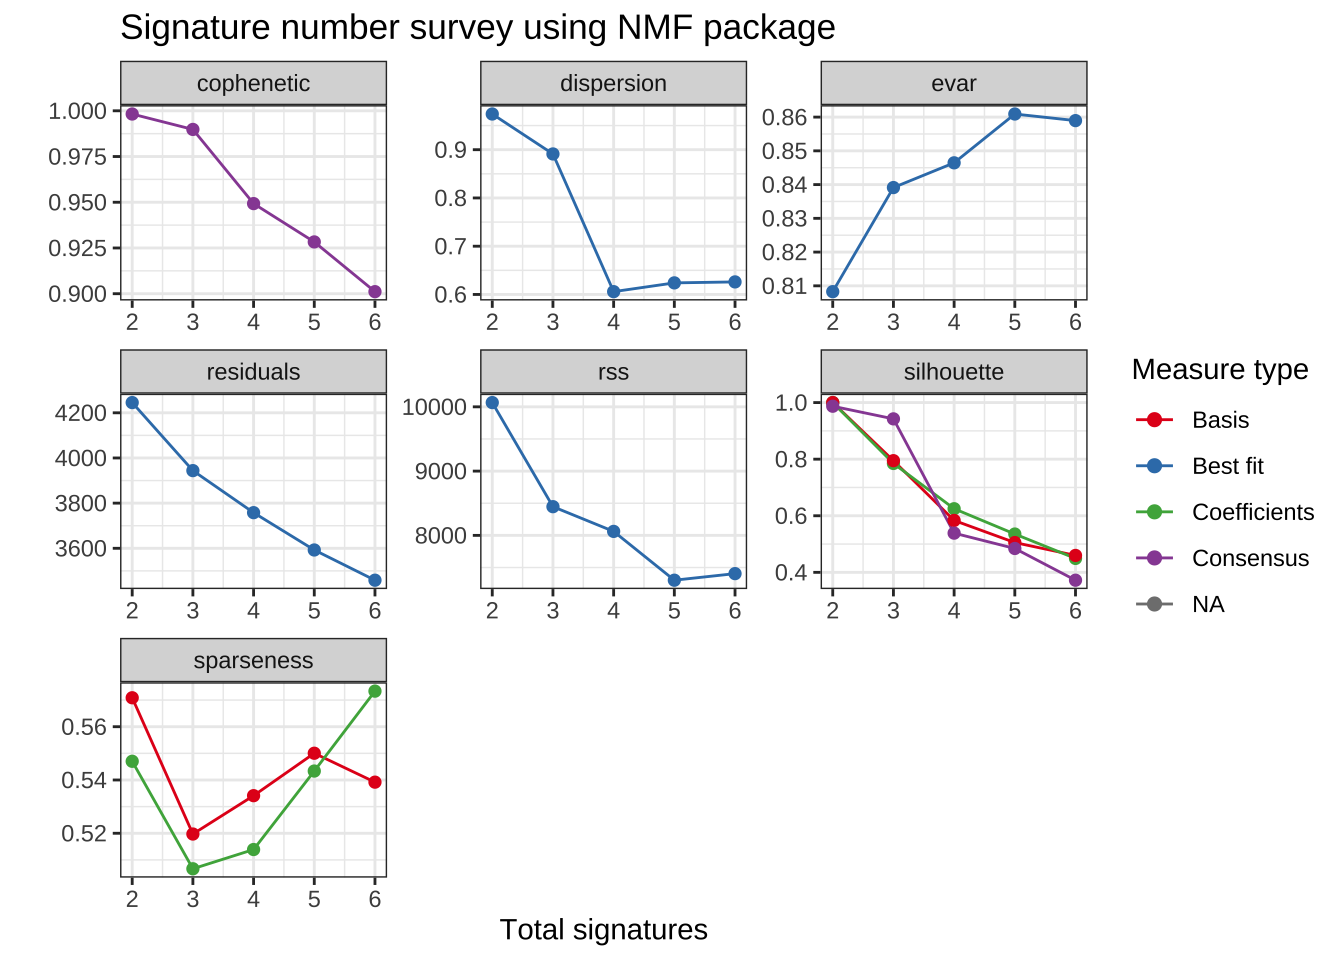
\includegraphics[width=0.95\linewidth]{sigminer_files/figure-latex/unnamed-chunk-33-1}

\begin{quote}
For the details of all the measures above, please read \citet{gaujoux2010flexible} and \href{https://cran.r-project.org/web/packages/NMF/vignettes/}{vignette} of R package \textbf{NMF}.
The measures either provide stability (\texttt{cophenetic}) or how well can be reconstructed (\texttt{rss}).
\end{quote}

Typically, measure \textbf{cophenetic} is used for determining the signature number. We can easily generate an elbow plot
with function \texttt{show\_sig\_number\_survey()}.

\begin{Shaded}
\begin{Highlighting}[]
\FunctionTok{show\_sig\_number\_survey}\NormalTok{(mt\_est}\SpecialCharTok{$}\NormalTok{survey, }\AttributeTok{right\_y =} \ConstantTok{NULL}\NormalTok{)}
\end{Highlighting}
\end{Shaded}

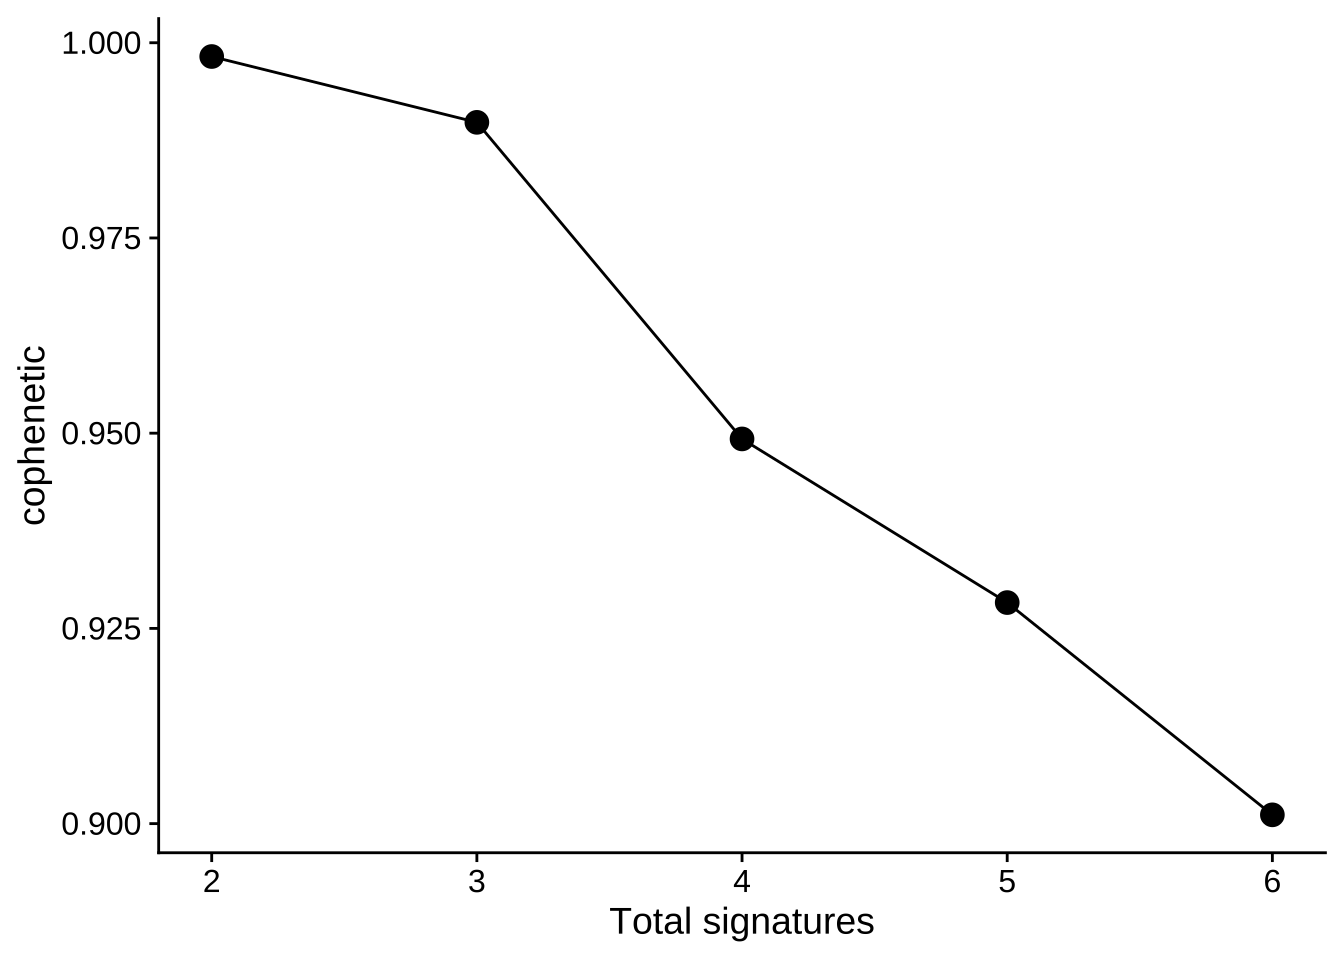
\includegraphics[width=0.95\linewidth]{sigminer_files/figure-latex/unnamed-chunk-34-1}

\begin{quote}
The most common approach is to use the cophenetic correlation coefficient. Brunet et al.~suggested choosing the smallest value of r for which this coefficient starts decreasing. \citep{gaujoux2010flexible}
Cophenetic value (range from 0-1) indicates the robustness of consensus matrix clustering. In this situation, 3 is good. However, we can found that the cophenetic values are all \textgreater=0.9 from 2 to 5. So the more suitable way is considering both stability and reconstruction error at the same time, it can be easily done by \texttt{show\_sig\_number\_survey()}.
\end{quote}

\begin{Shaded}
\begin{Highlighting}[]
\FunctionTok{show\_sig\_number\_survey}\NormalTok{(mt\_est}\SpecialCharTok{$}\NormalTok{survey)}
\end{Highlighting}
\end{Shaded}

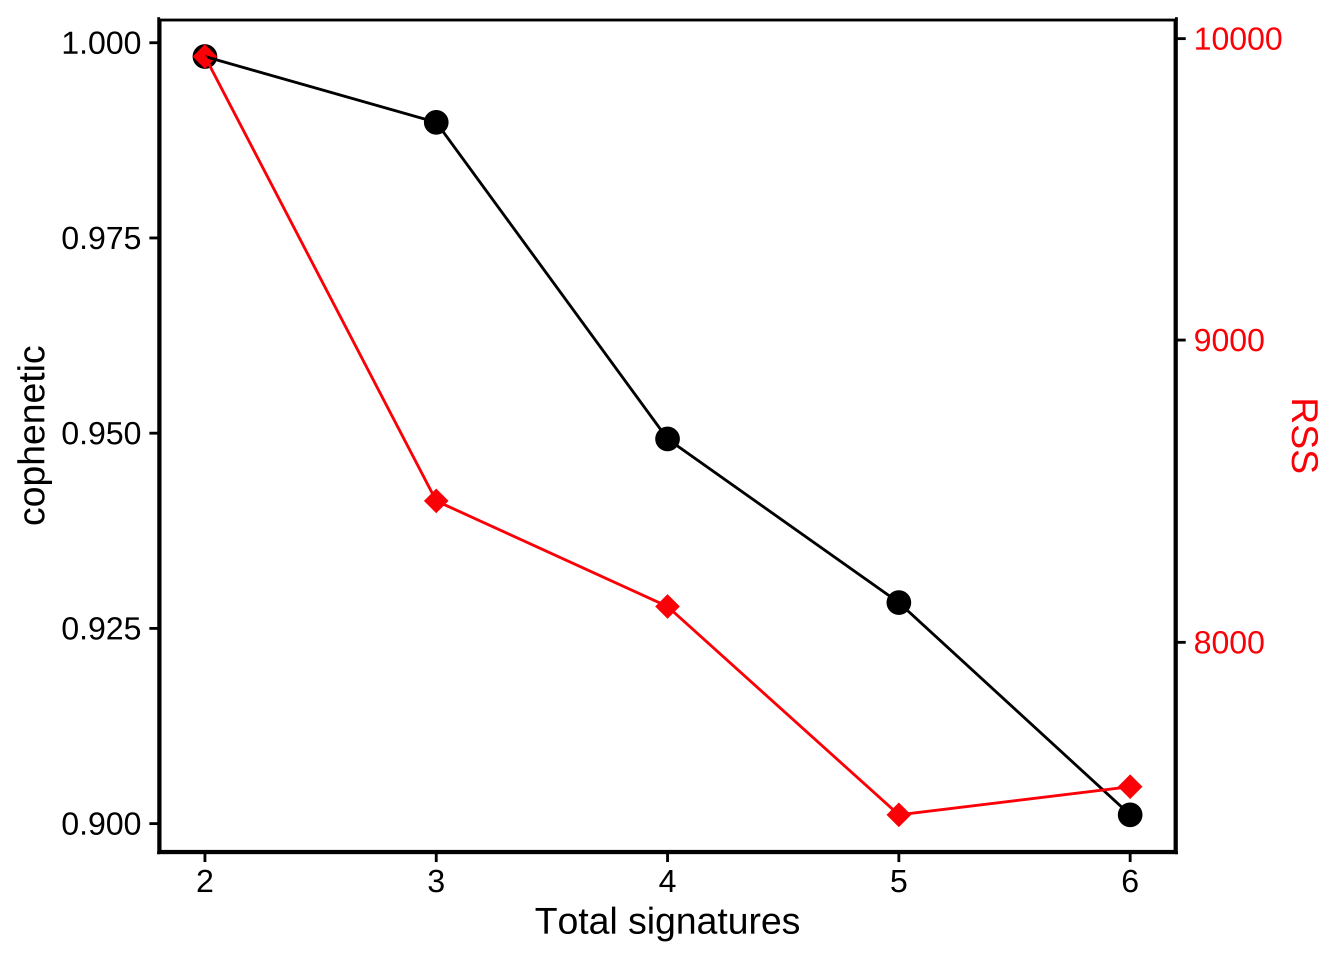
\includegraphics[width=0.95\linewidth]{sigminer_files/figure-latex/unnamed-chunk-35-1}

\begin{quote}
This function is very flexible, you can pick up any measure to the left/right axis. However, the default setting is the most recommended way.
We can see that we get a minimal RSS in signature number, and when this value goes from 5 to 6, the RSS increase! So we should not choose signature number more than 5 here because 6 is overfitting.
\end{quote}

\textbf{NOTE}: There are no gold standard to determine the signature number. Sometimes, you should consider multiple measures. Remember, the most important thing is that \textbf{you should have a good biological explanation for each signature}.
The best solution in study may not be the best solution in math.

Now that the 5 signatures should be a stable solution, next we can extract it with
more runs to obtain the optimal result. In general, use 30\textasciitilde50 NMF runs will get a robust result.

\begin{Shaded}
\begin{Highlighting}[]
\NormalTok{mt\_sig }\OtherTok{\textless{}{-}} \FunctionTok{sig\_extract}\NormalTok{(mt\_tally}\SpecialCharTok{$}\NormalTok{nmf\_matrix,}
  \AttributeTok{n\_sig =} \DecValTok{5}\NormalTok{,}
  \AttributeTok{nrun =} \DecValTok{30}\NormalTok{,}
  \AttributeTok{cores =} \DecValTok{4}
\NormalTok{)}
\end{Highlighting}
\end{Shaded}

\hypertarget{automatic-extraction}{%
\subsection{Automatic extraction}\label{automatic-extraction}}

If you have no idea to select an optimal signature number from procedures above, you can try auto-extraction approaches provided by \textbf{sigminer}.

The latest version of \textbf{sigminer} provides three ways to auto-extract mutational signatures.

\begin{enumerate}
\def\labelenumi{\arabic{enumi}.}
\tightlist
\item
  Auto-extract signatures by automatic relevance determination technique in non-negative matrix factorization \citep{tan2012automatic}, the code is implemented by \textbf{SignatureAnalyzer} \citep{kim2016somatic} and exported to \textbf{sigminer}. This approach is known as bayesian NMF and the default approach in \texttt{sig\_unify\_extract()}.
\item
  Auto-extract signatures by \href{https://github.com/AlexandrovLab/SigProfilerExtractor}{SigProfiler}, the gold-standard tool used for identifying signatures cataloged in COSMIC database. The technical details please read \citet{alexandrov2020repertoire}.
\item
  Multiple NMF runs with bootstrapped mutation catalogs. This method is adopted from \citet{degasperi2020practical}.
\end{enumerate}

\hypertarget{method-1-bayesian-nmf}{%
\subsubsection{Method 1: Bayesian NMF}\label{method-1-bayesian-nmf}}

In this approach, you need to set a maximum signature number (default is \texttt{25}) and run times to get the result. 10 for \texttt{nrun} here is okay, and more than 100 is not recommended.
The Bayesian NMF will starts from a larger signature number and reduce it to a proper signature number to maximize posterior probability.

\begin{Shaded}
\begin{Highlighting}[]
\NormalTok{mt\_sig2 }\OtherTok{\textless{}{-}} \FunctionTok{sig\_unify\_extract}\NormalTok{(mt\_tally}\SpecialCharTok{$}\NormalTok{nmf\_matrix, }\AttributeTok{range =} \DecValTok{10}\NormalTok{, }\AttributeTok{nrun =} \DecValTok{10}\NormalTok{)}
\end{Highlighting}
\end{Shaded}

This is same as:

\begin{Shaded}
\begin{Highlighting}[]
\NormalTok{mt\_sig2 }\OtherTok{\textless{}{-}} \FunctionTok{sig\_auto\_extract}\NormalTok{(mt\_tally}\SpecialCharTok{$}\NormalTok{nmf\_matrix,}
  \AttributeTok{K0 =} \DecValTok{10}\NormalTok{, }\AttributeTok{nrun =} \DecValTok{10}\NormalTok{,}
  \AttributeTok{strategy =} \StringTok{"stable"}
\NormalTok{)}
\end{Highlighting}
\end{Shaded}

Here the program uses \textbf{`robust' strategy} to return the result (see \texttt{strategy} option). It means that if you run 10 times and 6 of them return \texttt{4} signatures, then the optimal result with \texttt{4} signatures will be returned.

The info of each run can be given as:

\begin{Shaded}
\begin{Highlighting}[]
\NormalTok{knitr}\SpecialCharTok{::}\FunctionTok{kable}\NormalTok{(mt\_sig2}\SpecialCharTok{$}\NormalTok{Raw}\SpecialCharTok{$}\NormalTok{summary\_run)}
\end{Highlighting}
\end{Shaded}

\begin{tabular}{r|r|r|l}
\hline
Run & K & posterior & file\\
\hline
5 & 3 & -1497.498 & /var/folders/qx/5tqxhrrd5xd\_n9rfbb\_m5c200000gn/T//RtmpPz6VVL/BayesNMF.5.rds\\
\hline
3 & 3 & -1497.752 & /var/folders/qx/5tqxhrrd5xd\_n9rfbb\_m5c200000gn/T//RtmpPz6VVL/BayesNMF.3.rds\\
\hline
7 & 3 & -1497.841 & /var/folders/qx/5tqxhrrd5xd\_n9rfbb\_m5c200000gn/T//RtmpPz6VVL/BayesNMF.7.rds\\
\hline
1 & 3 & -1498.525 & /var/folders/qx/5tqxhrrd5xd\_n9rfbb\_m5c200000gn/T//RtmpPz6VVL/BayesNMF.1.rds\\
\hline
9 & 3 & -1498.528 & /var/folders/qx/5tqxhrrd5xd\_n9rfbb\_m5c200000gn/T//RtmpPz6VVL/BayesNMF.9.rds\\
\hline
10 & 3 & -1498.883 & /var/folders/qx/5tqxhrrd5xd\_n9rfbb\_m5c200000gn/T//RtmpPz6VVL/BayesNMF.10.rds\\
\hline
6 & 3 & -1499.748 & /var/folders/qx/5tqxhrrd5xd\_n9rfbb\_m5c200000gn/T//RtmpPz6VVL/BayesNMF.6.rds\\
\hline
4 & 3 & -1499.814 & /var/folders/qx/5tqxhrrd5xd\_n9rfbb\_m5c200000gn/T//RtmpPz6VVL/BayesNMF.4.rds\\
\hline
8 & 3 & -1500.195 & /var/folders/qx/5tqxhrrd5xd\_n9rfbb\_m5c200000gn/T//RtmpPz6VVL/BayesNMF.8.rds\\
\hline
2 & 4 & -1604.000 & /var/folders/qx/5tqxhrrd5xd\_n9rfbb\_m5c200000gn/T//RtmpPz6VVL/BayesNMF.2.rds\\
\hline
\end{tabular}

The \texttt{mt\_sig2} has similar structure as \texttt{mut\_sig}.

\hypertarget{method-2-sigprofiler}{%
\subsubsection{Method 2: SigProfiler}\label{method-2-sigprofiler}}

\textbf{Sigminer} provides two functions \texttt{sigprofiler\_extract()} and \texttt{sigprofiler\_import()} to install, use SigProfiler and import \href{https://github.com/AlexandrovLab/SigProfilerExtractor}{\textbf{SigProfilerExtractor}} results into R as a \texttt{Signature} object like other extraction methods mentioned above.

An (not running) example is given below (see \texttt{?sigprofiler} for more info).

\begin{Shaded}
\begin{Highlighting}[]
\NormalTok{reticulate}\SpecialCharTok{::}\FunctionTok{conda\_list}\NormalTok{()}
\FunctionTok{sigprofiler\_extract}\NormalTok{(cn\_tally\_W}\SpecialCharTok{$}\NormalTok{nmf\_matrix, }\StringTok{"\textasciitilde{}/test/test\_sigminer"}\NormalTok{,}
  \AttributeTok{use\_conda =} \ConstantTok{TRUE}
\NormalTok{)}

\CommentTok{\# Same as}
\CommentTok{\# sig\_unify\_extract(mt\_tally$nmf\_matrix, use\_conda = FALSE, py\_path = "/Users/wsx/anaconda3/bin/python", approach = "sigprofiler", out = "\textasciitilde{}/test/test\_sigminer")}
\FunctionTok{sigprofiler\_extract}\NormalTok{(mt\_tally}\SpecialCharTok{$}\NormalTok{nmf\_matrix, }\StringTok{"\textasciitilde{}/test/test\_sigminer"}\NormalTok{,}
  \AttributeTok{use\_conda =} \ConstantTok{FALSE}\NormalTok{, }\AttributeTok{py\_path =} \StringTok{"/Users/wsx/anaconda3/bin/python"}
\NormalTok{)}
\end{Highlighting}
\end{Shaded}

\hypertarget{method-3-bootstrapped-nmf}{%
\subsubsection{Method 3: bootstrapped NMF}\label{method-3-bootstrapped-nmf}}

\begin{Shaded}
\begin{Highlighting}[]
\CommentTok{\# Same as}
\CommentTok{\# mt\_sig3 \textless{}{-} sig\_unify\_extract(}
\CommentTok{\#   cn\_tally\_W$nmf\_matrix,}
\CommentTok{\#   range = 3:8,}
\CommentTok{\#   nrun = 10}
\CommentTok{\#   n\_bootstrap = 5}
\CommentTok{\# )}

\NormalTok{mt\_sig3 }\OtherTok{\textless{}{-}} \FunctionTok{bp\_extract\_signatures}\NormalTok{(}
\NormalTok{  cn\_tally\_W}\SpecialCharTok{$}\NormalTok{nmf\_matrix,}
  \AttributeTok{range =} \DecValTok{3}\SpecialCharTok{:}\DecValTok{8}\NormalTok{,}
  \AttributeTok{n\_bootstrap =} \DecValTok{5}\NormalTok{,}
  \AttributeTok{n\_nmf\_run =} \DecValTok{10}
\NormalTok{)}
\end{Highlighting}
\end{Shaded}

\hypertarget{match-signatures}{%
\section{Match Signatures}\label{match-signatures}}

After extracting signatures, we need to know their etiologies. This can be done by comparing the identified signatures and reference signatures from COSMIC database.

\begin{Shaded}
\begin{Highlighting}[]
\NormalTok{sim }\OtherTok{\textless{}{-}} \FunctionTok{get\_sig\_similarity}\NormalTok{(mt\_sig2)}
\DocumentationTok{\#\# {-}Comparing against COSMIC signatures}
\DocumentationTok{\#\# {-}{-}{-}{-}{-}{-}{-}{-}{-}{-}{-}{-}{-}{-}{-}{-}{-}{-}{-}{-}{-}{-}{-}{-}{-}{-}{-}{-}{-}{-}{-}{-}{-}{-}{-}{-}}
\DocumentationTok{\#\# {-}{-}Found Sig1 most similar to COSMIC\_3}
\DocumentationTok{\#\#    Aetiology: defects in DNA{-}DSB repair by HR [similarity: 0.826]}
\DocumentationTok{\#\# {-}{-}Found Sig2 most similar to COSMIC\_1}
\DocumentationTok{\#\#    Aetiology: spontaneous deamination of 5{-}methylcytosine [similarity: 0.944]}
\DocumentationTok{\#\# {-}{-}Found Sig3 most similar to COSMIC\_2}
\DocumentationTok{\#\#    Aetiology: APOBEC Cytidine Deaminase (C\textgreater{}T) [similarity: 0.838]}
\DocumentationTok{\#\# {-}{-}{-}{-}{-}{-}{-}{-}{-}{-}{-}{-}{-}{-}{-}{-}{-}{-}{-}{-}{-}{-}{-}{-}{-}{-}{-}{-}{-}{-}{-}{-}{-}{-}{-}{-}}
\DocumentationTok{\#\# Return result invisiblely.}
\end{Highlighting}
\end{Shaded}

The result object \texttt{sim} is a list.

\begin{Shaded}
\begin{Highlighting}[]
\FunctionTok{str}\NormalTok{(sim)}
\DocumentationTok{\#\# List of 4}
\DocumentationTok{\#\#  $ similarity  : num [1:3, 1:30] 0.826 0.274 0.373 0.56 0.944 0.164 0.088 0.259 0.838 0.722 ...}
\DocumentationTok{\#\#   ..{-} attr(*, "dimnames")=List of 2}
\DocumentationTok{\#\#   .. ..$ : chr [1:3] "Sig1" "Sig2" "Sig3"}
\DocumentationTok{\#\#   .. ..$ : chr [1:30] "COSMIC\_3" "COSMIC\_1" "COSMIC\_2" "COSMIC\_4" ...}
\DocumentationTok{\#\#  $ aetiology\_db:List of 1}
\DocumentationTok{\#\#   ..$ : chr [1:30] "spontaneous deamination of 5{-}methylcytosine" "APOBEC Cytidine Deaminase (C\textgreater{}T)" "defects in DNA{-}DSB repair by HR" "exposure to tobacco (smoking) mutagens" ...}
\DocumentationTok{\#\#  $ best\_match  :List of 3}
\DocumentationTok{\#\#   ..$ Sig1:List of 2}
\DocumentationTok{\#\#   .. ..$ aetiology : chr "defects in DNA{-}DSB repair by HR"}
\DocumentationTok{\#\#   .. ..$ best\_match: chr "Best match: COSMIC\_3 [similarity: 0.826]"}
\DocumentationTok{\#\#   ..$ Sig2:List of 2}
\DocumentationTok{\#\#   .. ..$ aetiology : chr "spontaneous deamination of 5{-}methylcytosine"}
\DocumentationTok{\#\#   .. ..$ best\_match: chr "Best match: COSMIC\_1 [similarity: 0.944]"}
\DocumentationTok{\#\#   ..$ Sig3:List of 2}
\DocumentationTok{\#\#   .. ..$ aetiology : chr "APOBEC Cytidine Deaminase (C\textgreater{}T)"}
\DocumentationTok{\#\#   .. ..$ best\_match: chr "Best match: COSMIC\_2 [similarity: 0.838]"}
\DocumentationTok{\#\#  $ rss         : num [1:3, 1:30] 0.04294 0.00684 0.14741 0.24881 0.24076 ...}
\DocumentationTok{\#\#   ..{-} attr(*, "dimnames")=List of 2}
\DocumentationTok{\#\#   .. ..$ : chr [1:3] "Sig1" "Sig2" "Sig3"}
\DocumentationTok{\#\#   .. ..$ : chr [1:30] "COSMIC\_1" "COSMIC\_2" "COSMIC\_3" "COSMIC\_4" ...}
\DocumentationTok{\#\#  {-} attr(*, "class")= chr [1:2] "similarity" "list"}
\end{Highlighting}
\end{Shaded}

From the result we can see that three signatures are properly matched to COSMIC reference signatures. If you find unknown signatures in your study, you should explore the etiologies by other analyses and even experiments.

The similarity matrix can be plotted.

\begin{Shaded}
\begin{Highlighting}[]
\NormalTok{pheatmap}\SpecialCharTok{::}\FunctionTok{pheatmap}\NormalTok{(sim}\SpecialCharTok{$}\NormalTok{similarity)}
\end{Highlighting}
\end{Shaded}

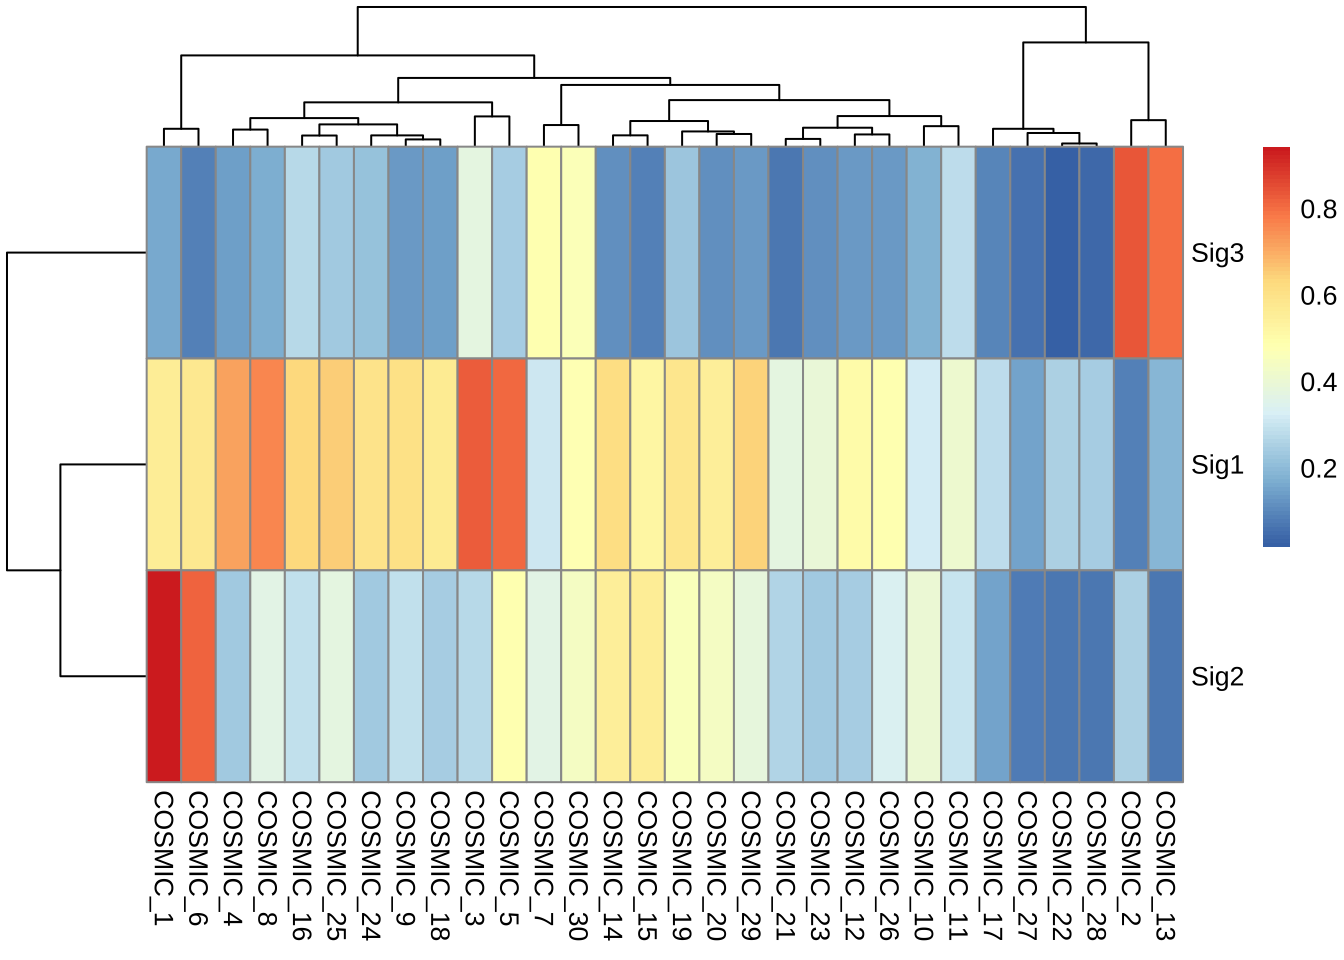
\includegraphics[width=0.95\linewidth]{sigminer_files/figure-latex/unnamed-chunk-46-1}

You can also try the COSMIC signature database V3 with:

\begin{Shaded}
\begin{Highlighting}[]
\NormalTok{sim\_v3 }\OtherTok{\textless{}{-}} \FunctionTok{get\_sig\_similarity}\NormalTok{(mt\_sig2, }\AttributeTok{sig\_db =} \StringTok{"SBS"}\NormalTok{)}
\DocumentationTok{\#\# {-}Comparing against COSMIC signatures}
\DocumentationTok{\#\# {-}{-}{-}{-}{-}{-}{-}{-}{-}{-}{-}{-}{-}{-}{-}{-}{-}{-}{-}{-}{-}{-}{-}{-}{-}{-}{-}{-}{-}{-}{-}{-}{-}{-}{-}{-}}
\DocumentationTok{\#\# {-}{-}Found Sig1 most similar to SBS3}
\DocumentationTok{\#\#    Aetiology: Defective homologous recombination DNA damage repair [similarity: 0.828]}
\DocumentationTok{\#\# {-}{-}Found Sig2 most similar to SBS1}
\DocumentationTok{\#\#    Aetiology: Spontaneous deamination of 5{-}methylcytosine (clock{-}like signature) [similarity: 0.876]}
\DocumentationTok{\#\# {-}{-}Found Sig3 most similar to SBS2}
\DocumentationTok{\#\#    Aetiology: Activity of APOBEC family of cytidine deaminases [similarity: 0.746]}
\DocumentationTok{\#\# {-}{-}{-}{-}{-}{-}{-}{-}{-}{-}{-}{-}{-}{-}{-}{-}{-}{-}{-}{-}{-}{-}{-}{-}{-}{-}{-}{-}{-}{-}{-}{-}{-}{-}{-}{-}}
\DocumentationTok{\#\# Return result invisiblely.}
\end{Highlighting}
\end{Shaded}

\hypertarget{reference-signature-fitting}{%
\section{Reference signature fitting}\label{reference-signature-fitting}}

Besides \emph{de novo} signature discovery shown in previous chapters, another common task is that
you have gotten some reference signatures (either from known database like COSMIC or \emph{de novo} discovery step), you want to know how these signatures contribute (fit) in a sample. That's the target of \texttt{sig\_fit()}.

\texttt{sig\_fit()} uses multiple methods to compute exposure of pre-defined signatures from the spectrum of a (can be more) sample. Use \texttt{?sig\_fit} see more detail.

To show how this function works, we use a sample with maximum mutation counts as example data.

\begin{Shaded}
\begin{Highlighting}[]
\NormalTok{i }\OtherTok{\textless{}{-}} \FunctionTok{which.max}\NormalTok{(}\FunctionTok{apply}\NormalTok{(mt\_tally}\SpecialCharTok{$}\NormalTok{nmf\_matrix, }\DecValTok{1}\NormalTok{, sum))}
\NormalTok{example\_mat }\OtherTok{\textless{}{-}}\NormalTok{ mt\_tally}\SpecialCharTok{$}\NormalTok{nmf\_matrix[i, , drop }\OtherTok{=} \ConstantTok{FALSE}\NormalTok{] }\SpecialCharTok{\%\textgreater{}\%} \FunctionTok{t}\NormalTok{()}
\end{Highlighting}
\end{Shaded}

\begin{Shaded}
\begin{Highlighting}[]
\FunctionTok{head}\NormalTok{(example\_mat)}
\DocumentationTok{\#\#         TCGA{-}A8{-}A09G{-}01A{-}21W{-}A019{-}09}
\DocumentationTok{\#\# A[T\textgreater{}C]A                            1}
\DocumentationTok{\#\# C[T\textgreater{}C]A                            0}
\DocumentationTok{\#\# G[T\textgreater{}C]A                            1}
\DocumentationTok{\#\# T[T\textgreater{}C]A                            1}
\DocumentationTok{\#\# A[C\textgreater{}T]A                            5}
\DocumentationTok{\#\# C[C\textgreater{}T]A                            3}
\end{Highlighting}
\end{Shaded}

\hypertarget{fit-signatures-from-reference-signature-databasase}{%
\subsection{Fit signatures from reference signature databasase}\label{fit-signatures-from-reference-signature-databasase}}

For SBS signatures, users may want to directly use reference signatures from COSMIC database.

\begin{Shaded}
\begin{Highlighting}[]
\FunctionTok{sig\_fit}\NormalTok{(example\_mat, }\AttributeTok{sig\_index =} \DecValTok{1}\SpecialCharTok{:}\DecValTok{30}\NormalTok{)}
\DocumentationTok{\#\# i [2022{-}08{-}29 11:08:15]: Started.}
\DocumentationTok{\#\# v [2022{-}08{-}29 11:08:15]: Signature index detected.}
\DocumentationTok{\#\# i [2022{-}08{-}29 11:08:15]: Checking signature database in package.}
\DocumentationTok{\#\# i [2022{-}08{-}29 11:08:15]: Checking signature index.}
\DocumentationTok{\#\# i [2022{-}08{-}29 11:08:15]: Valid index for db \textquotesingle{}legacy\textquotesingle{}:}
\DocumentationTok{\#\# 1 2 3 4 5 6 7 8 9 10 11 12 13 14 15 16 17 18 19 20 21 22 23 24 25 26 27 28 29 30}
\DocumentationTok{\#\# v [2022{-}08{-}29 11:08:15]: Database and index checked.}
\DocumentationTok{\#\# v [2022{-}08{-}29 11:08:15]: Signature normalized.}
\DocumentationTok{\#\# i [2022{-}08{-}29 11:08:15]: Checking row number for catalog matrix and signature matrix.}
\DocumentationTok{\#\# v [2022{-}08{-}29 11:08:15]: Checked.}
\DocumentationTok{\#\# i [2022{-}08{-}29 11:08:15]: Checking rownames for catalog matrix and signature matrix.}
\DocumentationTok{\#\# i [2022{-}08{-}29 11:08:15]: Matrix V and W don\textquotesingle{}t have same orders. Try reordering...}
\DocumentationTok{\#\# v [2022{-}08{-}29 11:08:15]: Checked.}
\DocumentationTok{\#\# v [2022{-}08{-}29 11:08:15]: Method \textquotesingle{}QP\textquotesingle{} detected.}
\DocumentationTok{\#\# v [2022{-}08{-}29 11:08:15]: Corresponding function generated.}
\DocumentationTok{\#\# i [2022{-}08{-}29 11:08:15]: Calling function.}
\DocumentationTok{\#\# i [2022{-}08{-}29 11:08:15]: Fitting sample: TCGA{-}A8{-}A09G{-}01A{-}21W{-}A019{-}09}
\DocumentationTok{\#\# v [2022{-}08{-}29 11:08:15]: Done.}
\DocumentationTok{\#\# i [2022{-}08{-}29 11:08:15]: Generating output signature exposures.}
\DocumentationTok{\#\# v [2022{-}08{-}29 11:08:15]: Done.}
\DocumentationTok{\#\# i [2022{-}08{-}29 11:08:15]: 0.063 secs elapsed.}
\DocumentationTok{\#\#           TCGA{-}A8{-}A09G{-}01A{-}21W{-}A019{-}09}
\DocumentationTok{\#\# COSMIC\_1                     24.215933}
\DocumentationTok{\#\# COSMIC\_2                    127.164108}
\DocumentationTok{\#\# COSMIC\_3                      0.000000}
\DocumentationTok{\#\# COSMIC\_4                      0.000000}
\DocumentationTok{\#\# COSMIC\_5                      0.000000}
\DocumentationTok{\#\# COSMIC\_6                      0.000000}
\DocumentationTok{\#\# COSMIC\_7                      4.907674}
\DocumentationTok{\#\# COSMIC\_8                      0.000000}
\DocumentationTok{\#\# COSMIC\_9                      0.000000}
\DocumentationTok{\#\# COSMIC\_10                     3.584276}
\DocumentationTok{\#\# COSMIC\_11                     0.000000}
\DocumentationTok{\#\# COSMIC\_12                    11.062526}
\DocumentationTok{\#\# COSMIC\_13                   168.298139}
\DocumentationTok{\#\# COSMIC\_14                     0.000000}
\DocumentationTok{\#\# COSMIC\_15                     0.000000}
\DocumentationTok{\#\# COSMIC\_16                     0.000000}
\DocumentationTok{\#\# COSMIC\_17                     5.578495}
\DocumentationTok{\#\# COSMIC\_18                     0.000000}
\DocumentationTok{\#\# COSMIC\_19                     0.000000}
\DocumentationTok{\#\# COSMIC\_20                     0.000000}
\DocumentationTok{\#\# COSMIC\_21                     0.000000}
\DocumentationTok{\#\# COSMIC\_22                     0.000000}
\DocumentationTok{\#\# COSMIC\_23                     0.000000}
\DocumentationTok{\#\# COSMIC\_24                    12.084656}
\DocumentationTok{\#\# COSMIC\_25                     0.000000}
\DocumentationTok{\#\# COSMIC\_26                     0.000000}
\DocumentationTok{\#\# COSMIC\_27                     0.000000}
\DocumentationTok{\#\# COSMIC\_28                     0.000000}
\DocumentationTok{\#\# COSMIC\_29                     0.000000}
\DocumentationTok{\#\# COSMIC\_30                     0.104192}
\end{Highlighting}
\end{Shaded}

\begin{quote}
At default, COSMIC v2 signature database with 30 reference signatures is used (i.e.~\texttt{sig\_db\ =\ "legacy"}). Set \texttt{sig\_db\ =\ "SBS"} for COSMIC v3 signature database.
That's it!
\end{quote}

You can set \texttt{type\ =\ "relative"} for getting relative exposure.

\begin{Shaded}
\begin{Highlighting}[]
\FunctionTok{sig\_fit}\NormalTok{(example\_mat, }\AttributeTok{sig\_index =} \DecValTok{1}\SpecialCharTok{:}\DecValTok{30}\NormalTok{, }\AttributeTok{type =} \StringTok{"relative"}\NormalTok{)}
\DocumentationTok{\#\# i [2022{-}08{-}29 11:08:15]: Started.}
\DocumentationTok{\#\# v [2022{-}08{-}29 11:08:15]: Signature index detected.}
\DocumentationTok{\#\# i [2022{-}08{-}29 11:08:15]: Checking signature database in package.}
\DocumentationTok{\#\# i [2022{-}08{-}29 11:08:15]: Checking signature index.}
\DocumentationTok{\#\# i [2022{-}08{-}29 11:08:15]: Valid index for db \textquotesingle{}legacy\textquotesingle{}:}
\DocumentationTok{\#\# 1 2 3 4 5 6 7 8 9 10 11 12 13 14 15 16 17 18 19 20 21 22 23 24 25 26 27 28 29 30}
\DocumentationTok{\#\# v [2022{-}08{-}29 11:08:15]: Database and index checked.}
\DocumentationTok{\#\# v [2022{-}08{-}29 11:08:15]: Signature normalized.}
\DocumentationTok{\#\# i [2022{-}08{-}29 11:08:15]: Checking row number for catalog matrix and signature matrix.}
\DocumentationTok{\#\# v [2022{-}08{-}29 11:08:15]: Checked.}
\DocumentationTok{\#\# i [2022{-}08{-}29 11:08:15]: Checking rownames for catalog matrix and signature matrix.}
\DocumentationTok{\#\# i [2022{-}08{-}29 11:08:15]: Matrix V and W don\textquotesingle{}t have same orders. Try reordering...}
\DocumentationTok{\#\# v [2022{-}08{-}29 11:08:15]: Checked.}
\DocumentationTok{\#\# v [2022{-}08{-}29 11:08:15]: Method \textquotesingle{}QP\textquotesingle{} detected.}
\DocumentationTok{\#\# v [2022{-}08{-}29 11:08:15]: Corresponding function generated.}
\DocumentationTok{\#\# i [2022{-}08{-}29 11:08:15]: Calling function.}
\DocumentationTok{\#\# i [2022{-}08{-}29 11:08:15]: Fitting sample: TCGA{-}A8{-}A09G{-}01A{-}21W{-}A019{-}09}
\DocumentationTok{\#\# v [2022{-}08{-}29 11:08:15]: Done.}
\DocumentationTok{\#\# i [2022{-}08{-}29 11:08:15]: Generating output signature exposures.}
\DocumentationTok{\#\# v [2022{-}08{-}29 11:08:15]: Done.}
\DocumentationTok{\#\# i [2022{-}08{-}29 11:08:15]: 0.063 secs elapsed.}
\DocumentationTok{\#\#           TCGA{-}A8{-}A09G{-}01A{-}21W{-}A019{-}09}
\DocumentationTok{\#\# COSMIC\_1                      0.067832}
\DocumentationTok{\#\# COSMIC\_2                      0.356202}
\DocumentationTok{\#\# COSMIC\_3                      0.000000}
\DocumentationTok{\#\# COSMIC\_4                      0.000000}
\DocumentationTok{\#\# COSMIC\_5                      0.000000}
\DocumentationTok{\#\# COSMIC\_6                      0.000000}
\DocumentationTok{\#\# COSMIC\_7                      0.013747}
\DocumentationTok{\#\# COSMIC\_8                      0.000000}
\DocumentationTok{\#\# COSMIC\_9                      0.000000}
\DocumentationTok{\#\# COSMIC\_10                     0.010040}
\DocumentationTok{\#\# COSMIC\_11                     0.000000}
\DocumentationTok{\#\# COSMIC\_12                     0.030987}
\DocumentationTok{\#\# COSMIC\_13                     0.471423}
\DocumentationTok{\#\# COSMIC\_14                     0.000000}
\DocumentationTok{\#\# COSMIC\_15                     0.000000}
\DocumentationTok{\#\# COSMIC\_16                     0.000000}
\DocumentationTok{\#\# COSMIC\_17                     0.015626}
\DocumentationTok{\#\# COSMIC\_18                     0.000000}
\DocumentationTok{\#\# COSMIC\_19                     0.000000}
\DocumentationTok{\#\# COSMIC\_20                     0.000000}
\DocumentationTok{\#\# COSMIC\_21                     0.000000}
\DocumentationTok{\#\# COSMIC\_22                     0.000000}
\DocumentationTok{\#\# COSMIC\_23                     0.000000}
\DocumentationTok{\#\# COSMIC\_24                     0.033851}
\DocumentationTok{\#\# COSMIC\_25                     0.000000}
\DocumentationTok{\#\# COSMIC\_26                     0.000000}
\DocumentationTok{\#\# COSMIC\_27                     0.000000}
\DocumentationTok{\#\# COSMIC\_28                     0.000000}
\DocumentationTok{\#\# COSMIC\_29                     0.000000}
\DocumentationTok{\#\# COSMIC\_30                     0.000292}
\end{Highlighting}
\end{Shaded}

For multiple samples, you can return a \texttt{data.table}, it can be easier to integrate with other information in R.

\begin{Shaded}
\begin{Highlighting}[]
\FunctionTok{sig\_fit}\NormalTok{(}\FunctionTok{t}\NormalTok{(mt\_tally}\SpecialCharTok{$}\NormalTok{nmf\_matrix[}\DecValTok{1}\SpecialCharTok{:}\DecValTok{5}\NormalTok{, ]), }\AttributeTok{sig\_index =} \DecValTok{1}\SpecialCharTok{:}\DecValTok{30}\NormalTok{, }\AttributeTok{return\_class =} \StringTok{"data.table"}\NormalTok{, }\AttributeTok{rel\_threshold =} \FloatTok{0.05}\NormalTok{)}
\DocumentationTok{\#\# i [2022{-}08{-}29 11:08:15]: Started.}
\DocumentationTok{\#\# v [2022{-}08{-}29 11:08:15]: Signature index detected.}
\DocumentationTok{\#\# i [2022{-}08{-}29 11:08:15]: Checking signature database in package.}
\DocumentationTok{\#\# i [2022{-}08{-}29 11:08:15]: Checking signature index.}
\DocumentationTok{\#\# i [2022{-}08{-}29 11:08:15]: Valid index for db \textquotesingle{}legacy\textquotesingle{}:}
\DocumentationTok{\#\# 1 2 3 4 5 6 7 8 9 10 11 12 13 14 15 16 17 18 19 20 21 22 23 24 25 26 27 28 29 30}
\DocumentationTok{\#\# v [2022{-}08{-}29 11:08:15]: Database and index checked.}
\DocumentationTok{\#\# v [2022{-}08{-}29 11:08:15]: Signature normalized.}
\DocumentationTok{\#\# i [2022{-}08{-}29 11:08:15]: Checking row number for catalog matrix and signature matrix.}
\DocumentationTok{\#\# v [2022{-}08{-}29 11:08:15]: Checked.}
\DocumentationTok{\#\# i [2022{-}08{-}29 11:08:15]: Checking rownames for catalog matrix and signature matrix.}
\DocumentationTok{\#\# i [2022{-}08{-}29 11:08:15]: Matrix V and W don\textquotesingle{}t have same orders. Try reordering...}
\DocumentationTok{\#\# v [2022{-}08{-}29 11:08:15]: Checked.}
\DocumentationTok{\#\# v [2022{-}08{-}29 11:08:15]: Method \textquotesingle{}QP\textquotesingle{} detected.}
\DocumentationTok{\#\# v [2022{-}08{-}29 11:08:15]: Corresponding function generated.}
\DocumentationTok{\#\# i [2022{-}08{-}29 11:08:15]: Calling function.}
\DocumentationTok{\#\# i [2022{-}08{-}29 11:08:15]: Fitting sample: TCGA{-}A1{-}A0SH{-}01A{-}11D{-}A099{-}09}
\DocumentationTok{\#\# i [2022{-}08{-}29 11:08:15]: Fitting sample: TCGA{-}A2{-}A04N{-}01A{-}11D{-}A10Y{-}09}
\DocumentationTok{\#\# i [2022{-}08{-}29 11:08:15]: Fitting sample: TCGA{-}A2{-}A0CP{-}01A{-}11W{-}A050{-}09}
\DocumentationTok{\#\# i [2022{-}08{-}29 11:08:15]: Fitting sample: TCGA{-}A2{-}A0EP{-}01A{-}52D{-}A22X{-}09}
\DocumentationTok{\#\# i [2022{-}08{-}29 11:08:15]: Fitting sample: TCGA{-}A2{-}A0EV{-}01A{-}11W{-}A050{-}09}
\DocumentationTok{\#\# v [2022{-}08{-}29 11:08:15]: Done.}
\DocumentationTok{\#\# i [2022{-}08{-}29 11:08:15]: Generating output signature exposures.}
\DocumentationTok{\#\# v [2022{-}08{-}29 11:08:15]: Done.}
\DocumentationTok{\#\# i [2022{-}08{-}29 11:08:15]: 0.091 secs elapsed.}
\DocumentationTok{\#\#                          sample  COSMIC\_1  COSMIC\_2 COSMIC\_3 COSMIC\_4 COSMIC\_5}
\DocumentationTok{\#\# 1: TCGA{-}A1{-}A0SH{-}01A{-}11D{-}A099{-}09  0.000000 37.420603 13.78689 0.000000        0}
\DocumentationTok{\#\# 2: TCGA{-}A2{-}A04N{-}01A{-}11D{-}A10Y{-}09 20.039543  2.888675  0.00000 0.000000        0}
\DocumentationTok{\#\# 3: TCGA{-}A2{-}A0CP{-}01A{-}11W{-}A050{-}09  3.648658  0.000000  0.00000 7.083113        0}
\DocumentationTok{\#\# 4: TCGA{-}A2{-}A0EP{-}01A{-}52D{-}A22X{-}09  0.000000  0.000000  0.00000 2.492218        0}
\DocumentationTok{\#\# 5: TCGA{-}A2{-}A0EV{-}01A{-}11W{-}A050{-}09  6.458422  0.000000 14.83102 0.000000        0}
\DocumentationTok{\#\#    COSMIC\_6  COSMIC\_7 COSMIC\_8 COSMIC\_9 COSMIC\_10 COSMIC\_11 COSMIC\_12 COSMIC\_13}
\DocumentationTok{\#\# 1: 12.93472 21.332013  0.00000        0  0.000000         0  0.000000 31.306430}
\DocumentationTok{\#\# 2:  0.00000  6.865345 12.11501        0  0.000000         0  0.000000  0.000000}
\DocumentationTok{\#\# 3:  0.00000 10.348536  0.00000        0  0.000000         0  0.000000  0.000000}
\DocumentationTok{\#\# 4:  0.00000  2.156319  0.00000        0  0.000000         0  1.334731  4.654227}
\DocumentationTok{\#\# 5: 14.78142 21.963952  0.00000        0  7.978962         0  0.000000  5.713563}
\DocumentationTok{\#\#    COSMIC\_14 COSMIC\_15 COSMIC\_16 COSMIC\_17 COSMIC\_18 COSMIC\_19 COSMIC\_20}
\DocumentationTok{\#\# 1:  0.000000   0.00000         0         0 12.007682         0  0.000000}
\DocumentationTok{\#\# 2:  0.000000   0.00000         0         0  0.000000         0  7.516444}
\DocumentationTok{\#\# 3:  0.000000  18.37734         0         0  4.384106         0  0.000000}
\DocumentationTok{\#\# 4:  6.728415   0.00000         0         0  0.000000         0  0.000000}
\DocumentationTok{\#\# 5:  0.000000   0.00000         0         0  0.000000         0  0.000000}
\DocumentationTok{\#\#    COSMIC\_21 COSMIC\_22 COSMIC\_23 COSMIC\_24 COSMIC\_25 COSMIC\_26 COSMIC\_27}
\DocumentationTok{\#\# 1:  0.000000         0   0.00000         0         0         0         0}
\DocumentationTok{\#\# 2:  0.000000         0   0.00000         0         0         0         0}
\DocumentationTok{\#\# 3:  0.000000         0   0.00000         0         0         0         0}
\DocumentationTok{\#\# 4:  0.000000         0   1.26778         0         0         0         0}
\DocumentationTok{\#\# 5:  4.311951         0   0.00000         0         0         0         0}
\DocumentationTok{\#\#    COSMIC\_28 COSMIC\_29 COSMIC\_30}
\DocumentationTok{\#\# 1:         0  0.000000         0}
\DocumentationTok{\#\# 2:         0  0.000000         0}
\DocumentationTok{\#\# 3:         0  4.776321         0}
\DocumentationTok{\#\# 4:         0  0.000000         0}
\DocumentationTok{\#\# 5:         0  0.000000         0}
\end{Highlighting}
\end{Shaded}

When you set multiple signatures, we recommend setting \texttt{rel\_threshold} option, which will set exposure of a signature to \texttt{0} if its relative exposure in a sample less than the \texttt{rel\_threshold}.

\hypertarget{fit-custom-signatures}{%
\subsection{Fit custom signatures}\label{fit-custom-signatures}}

We have already determined the SBS signatures before. Here we can set them to \texttt{sig} option.

\begin{Shaded}
\begin{Highlighting}[]
\FunctionTok{sig\_fit}\NormalTok{(example\_mat, }\AttributeTok{sig =}\NormalTok{ mt\_sig2)}
\DocumentationTok{\#\# i [2022{-}08{-}29 11:08:15]: Started.}
\DocumentationTok{\#\# i [2022{-}08{-}29 11:08:15]: Signature index not detected.}
\DocumentationTok{\#\# v [2022{-}08{-}29 11:08:15]: Signature object detected.}
\DocumentationTok{\#\# v [2022{-}08{-}29 11:08:15]: Database and index checked.}
\DocumentationTok{\#\# v [2022{-}08{-}29 11:08:15]: Signature normalized.}
\DocumentationTok{\#\# i [2022{-}08{-}29 11:08:15]: Checking row number for catalog matrix and signature matrix.}
\DocumentationTok{\#\# v [2022{-}08{-}29 11:08:15]: Checked.}
\DocumentationTok{\#\# i [2022{-}08{-}29 11:08:15]: Checking rownames for catalog matrix and signature matrix.}
\DocumentationTok{\#\# v [2022{-}08{-}29 11:08:15]: Checked.}
\DocumentationTok{\#\# v [2022{-}08{-}29 11:08:15]: Method \textquotesingle{}QP\textquotesingle{} detected.}
\DocumentationTok{\#\# v [2022{-}08{-}29 11:08:15]: Corresponding function generated.}
\DocumentationTok{\#\# i [2022{-}08{-}29 11:08:15]: Calling function.}
\DocumentationTok{\#\# i [2022{-}08{-}29 11:08:15]: Fitting sample: TCGA{-}A8{-}A09G{-}01A{-}21W{-}A019{-}09}
\DocumentationTok{\#\# v [2022{-}08{-}29 11:08:15]: Done.}
\DocumentationTok{\#\# i [2022{-}08{-}29 11:08:15]: Generating output signature exposures.}
\DocumentationTok{\#\# v [2022{-}08{-}29 11:08:15]: Done.}
\DocumentationTok{\#\# i [2022{-}08{-}29 11:08:15]: 0.043 secs elapsed.}
\DocumentationTok{\#\#      TCGA{-}A8{-}A09G{-}01A{-}21W{-}A019{-}09}
\DocumentationTok{\#\# Sig1                            0}
\DocumentationTok{\#\# Sig2                            0}
\DocumentationTok{\#\# Sig3                          357}
\end{Highlighting}
\end{Shaded}

\hypertarget{performance-comparison}{%
\subsection{Performance comparison}\label{performance-comparison}}

Now that we can use \texttt{sig\_fit} for getting optimal exposures, we can compare the RSS between \textbf{raw matrix} and the \textbf{reconstructed matrix} either by NMF and \texttt{sig\_fit()}.

i.e.~

\[
RSS = \sum(\hat H - H)^2
\]

\begin{Shaded}
\begin{Highlighting}[]
\DocumentationTok{\#\# Exposure got from NMF}
\FunctionTok{sum}\NormalTok{((}\FunctionTok{apply}\NormalTok{(mt\_sig2}\SpecialCharTok{$}\NormalTok{Signature, }\DecValTok{2}\NormalTok{, }\ControlFlowTok{function}\NormalTok{(x) x }\SpecialCharTok{/} \FunctionTok{sum}\NormalTok{(x)) }\SpecialCharTok{\%*\%}\NormalTok{ mt\_sig2}\SpecialCharTok{$}\NormalTok{Exposure }\SpecialCharTok{{-}} \FunctionTok{t}\NormalTok{(mt\_tally}\SpecialCharTok{$}\NormalTok{nmf\_matrix))}\SpecialCharTok{\^{}}\DecValTok{2}\NormalTok{)}
\DocumentationTok{\#\# [1] 8890.449}
\end{Highlighting}
\end{Shaded}

\begin{Shaded}
\begin{Highlighting}[]
\DocumentationTok{\#\# Exposure optimized by sig\_fit}
\NormalTok{H\_estimate }\OtherTok{\textless{}{-}} \FunctionTok{apply}\NormalTok{(mt\_sig2}\SpecialCharTok{$}\NormalTok{Signature, }\DecValTok{2}\NormalTok{, }\ControlFlowTok{function}\NormalTok{(x) x }\SpecialCharTok{/} \FunctionTok{sum}\NormalTok{(x)) }\SpecialCharTok{\%*\%} \FunctionTok{sig\_fit}\NormalTok{(}\FunctionTok{t}\NormalTok{(mt\_tally}\SpecialCharTok{$}\NormalTok{nmf\_matrix), }\AttributeTok{sig =}\NormalTok{ mt\_sig2)}
\DocumentationTok{\#\# i [2022{-}08{-}29 11:08:16]: Started.}
\DocumentationTok{\#\# i [2022{-}08{-}29 11:08:16]: Signature index not detected.}
\DocumentationTok{\#\# v [2022{-}08{-}29 11:08:16]: Signature object detected.}
\DocumentationTok{\#\# v [2022{-}08{-}29 11:08:16]: Database and index checked.}
\DocumentationTok{\#\# v [2022{-}08{-}29 11:08:16]: Signature normalized.}
\DocumentationTok{\#\# i [2022{-}08{-}29 11:08:16]: Checking row number for catalog matrix and signature matrix.}
\DocumentationTok{\#\# v [2022{-}08{-}29 11:08:16]: Checked.}
\DocumentationTok{\#\# i [2022{-}08{-}29 11:08:16]: Checking rownames for catalog matrix and signature matrix.}
\DocumentationTok{\#\# v [2022{-}08{-}29 11:08:16]: Checked.}
\DocumentationTok{\#\# v [2022{-}08{-}29 11:08:16]: Method \textquotesingle{}QP\textquotesingle{} detected.}
\DocumentationTok{\#\# v [2022{-}08{-}29 11:08:16]: Corresponding function generated.}
\DocumentationTok{\#\# i [2022{-}08{-}29 11:08:16]: Calling function.}
\DocumentationTok{\#\# i [2022{-}08{-}29 11:08:16]: Fitting sample: TCGA{-}A1{-}A0SH{-}01A{-}11D{-}A099{-}09}
\DocumentationTok{\#\# i [2022{-}08{-}29 11:08:16]: Fitting sample: TCGA{-}A2{-}A04N{-}01A{-}11D{-}A10Y{-}09}
\DocumentationTok{\#\# i [2022{-}08{-}29 11:08:16]: Fitting sample: TCGA{-}A2{-}A0CP{-}01A{-}11W{-}A050{-}09}
\DocumentationTok{\#\# i [2022{-}08{-}29 11:08:16]: Fitting sample: TCGA{-}A2{-}A0EP{-}01A{-}52D{-}A22X{-}09}
\DocumentationTok{\#\# i [2022{-}08{-}29 11:08:16]: Fitting sample: TCGA{-}A2{-}A0EV{-}01A{-}11W{-}A050{-}09}
\DocumentationTok{\#\# i [2022{-}08{-}29 11:08:16]: Fitting sample: TCGA{-}A2{-}A0SX{-}01A{-}12D{-}A099{-}09}
\DocumentationTok{\#\# i [2022{-}08{-}29 11:08:16]: Fitting sample: TCGA{-}A2{-}A0T7{-}01A{-}21D{-}A099{-}09}
\DocumentationTok{\#\# i [2022{-}08{-}29 11:08:16]: Fitting sample: TCGA{-}A2{-}A0YF{-}01A{-}21D{-}A10G{-}09}
\DocumentationTok{\#\# i [2022{-}08{-}29 11:08:16]: Fitting sample: TCGA{-}A2{-}A25F{-}01A{-}11D{-}A167{-}09}
\DocumentationTok{\#\# i [2022{-}08{-}29 11:08:16]: Fitting sample: TCGA{-}A2{-}A3XW{-}01A{-}11D{-}A23C{-}09}
\DocumentationTok{\#\# i [2022{-}08{-}29 11:08:16]: Fitting sample: TCGA{-}A2{-}A4S1{-}01A{-}21D{-}A25Q{-}09}
\DocumentationTok{\#\# i [2022{-}08{-}29 11:08:16]: Fitting sample: TCGA{-}A7{-}A0D9{-}01A{-}31W{-}A071{-}09}
\DocumentationTok{\#\# i [2022{-}08{-}29 11:08:16]: Fitting sample: TCGA{-}A7{-}A13F{-}01A{-}11D{-}A12Q{-}09}
\DocumentationTok{\#\# i [2022{-}08{-}29 11:08:16]: Fitting sample: TCGA{-}A7{-}A5ZV{-}01A{-}11D{-}A28B{-}09}
\DocumentationTok{\#\# i [2022{-}08{-}29 11:08:16]: Fitting sample: TCGA{-}A8{-}A06P{-}01A{-}11W{-}A019{-}09}
\DocumentationTok{\#\# i [2022{-}08{-}29 11:08:16]: Fitting sample: TCGA{-}A8{-}A076{-}01A{-}21W{-}A019{-}09}
\DocumentationTok{\#\# i [2022{-}08{-}29 11:08:16]: Fitting sample: TCGA{-}A8{-}A07W{-}01A{-}11W{-}A019{-}09}
\DocumentationTok{\#\# i [2022{-}08{-}29 11:08:16]: Fitting sample: TCGA{-}A8{-}A084{-}01A{-}21W{-}A019{-}09}
\DocumentationTok{\#\# i [2022{-}08{-}29 11:08:16]: Fitting sample: TCGA{-}A8{-}A08S{-}01A{-}11W{-}A050{-}09}
\DocumentationTok{\#\# i [2022{-}08{-}29 11:08:16]: Fitting sample: TCGA{-}A8{-}A09G{-}01A{-}21W{-}A019{-}09}
\DocumentationTok{\#\# i [2022{-}08{-}29 11:08:16]: Fitting sample: TCGA{-}A8{-}A0A4{-}01A{-}11W{-}A019{-}09}
\DocumentationTok{\#\# i [2022{-}08{-}29 11:08:16]: Fitting sample: TCGA{-}A8{-}A0AB{-}01A{-}11W{-}A050{-}09}
\DocumentationTok{\#\# i [2022{-}08{-}29 11:08:16]: Fitting sample: TCGA{-}AC{-}A2B8{-}01A{-}11D{-}A17D{-}09}
\DocumentationTok{\#\# i [2022{-}08{-}29 11:08:16]: Fitting sample: TCGA{-}AC{-}A2FO{-}01A{-}11D{-}A17W{-}09}
\DocumentationTok{\#\# i [2022{-}08{-}29 11:08:16]: Fitting sample: TCGA{-}AC{-}A3YI{-}01A{-}21D{-}A23C{-}09}
\DocumentationTok{\#\# i [2022{-}08{-}29 11:08:16]: Fitting sample: TCGA{-}AC{-}A8OS{-}01A{-}12D{-}A41F{-}09}
\DocumentationTok{\#\# i [2022{-}08{-}29 11:08:16]: Fitting sample: TCGA{-}AN{-}A0FK{-}01A{-}11W{-}A050{-}09}
\DocumentationTok{\#\# i [2022{-}08{-}29 11:08:16]: Fitting sample: TCGA{-}AN{-}A0FT{-}01A{-}11W{-}A050{-}09}
\DocumentationTok{\#\# i [2022{-}08{-}29 11:08:16]: Fitting sample: TCGA{-}AN{-}A0XO{-}01A{-}11D{-}A10G{-}09}
\DocumentationTok{\#\# i [2022{-}08{-}29 11:08:16]: Fitting sample: TCGA{-}AO{-}A1KS{-}01A{-}11D{-}A13L{-}09}
\DocumentationTok{\#\# i [2022{-}08{-}29 11:08:16]: Fitting sample: TCGA{-}AQ{-}A54O{-}01A{-}11D{-}A25Q{-}09}
\DocumentationTok{\#\# i [2022{-}08{-}29 11:08:16]: Fitting sample: TCGA{-}AQ{-}A7U7{-}01A{-}22D{-}A351{-}09}
\DocumentationTok{\#\# i [2022{-}08{-}29 11:08:16]: Fitting sample: TCGA{-}AR{-}A0TP{-}01A{-}11D{-}A099{-}09}
\DocumentationTok{\#\# i [2022{-}08{-}29 11:08:16]: Fitting sample: TCGA{-}AR{-}A0U3{-}01A{-}11D{-}A10G{-}09}
\DocumentationTok{\#\# i [2022{-}08{-}29 11:08:16]: Fitting sample: TCGA{-}AR{-}A1AH{-}01A{-}11D{-}A12B{-}09}
\DocumentationTok{\#\# i [2022{-}08{-}29 11:08:16]: Fitting sample: TCGA{-}AR{-}A1AJ{-}01A{-}21D{-}A12Q{-}09}
\DocumentationTok{\#\# i [2022{-}08{-}29 11:08:16]: Fitting sample: TCGA{-}AR{-}A1AN{-}01A{-}11D{-}A12Q{-}09}
\DocumentationTok{\#\# i [2022{-}08{-}29 11:08:16]: Fitting sample: TCGA{-}AR{-}A24N{-}01A{-}11D{-}A167{-}09}
\DocumentationTok{\#\# i [2022{-}08{-}29 11:08:16]: Fitting sample: TCGA{-}AR{-}A252{-}01A{-}11D{-}A167{-}09}
\DocumentationTok{\#\# i [2022{-}08{-}29 11:08:16]: Fitting sample: TCGA{-}AR{-}A2LL{-}01A{-}11D{-}A17W{-}09}
\DocumentationTok{\#\# i [2022{-}08{-}29 11:08:16]: Fitting sample: TCGA{-}AR{-}A2LO{-}01A{-}31D{-}A18P{-}09}
\DocumentationTok{\#\# i [2022{-}08{-}29 11:08:16]: Fitting sample: TCGA{-}B6{-}A0IE{-}01A{-}11W{-}A050{-}09}
\DocumentationTok{\#\# i [2022{-}08{-}29 11:08:16]: Fitting sample: TCGA{-}B6{-}A0IM{-}01A{-}11W{-}A050{-}09}
\DocumentationTok{\#\# i [2022{-}08{-}29 11:08:16]: Fitting sample: TCGA{-}B6{-}A0IP{-}01A{-}11D{-}A045{-}09}
\DocumentationTok{\#\# i [2022{-}08{-}29 11:08:16]: Fitting sample: TCGA{-}B6{-}A0RV{-}01A{-}11D{-}A099{-}09}
\DocumentationTok{\#\# i [2022{-}08{-}29 11:08:16]: Fitting sample: TCGA{-}B6{-}A0WZ{-}01A{-}11D{-}A10G{-}09}
\DocumentationTok{\#\# i [2022{-}08{-}29 11:08:16]: Fitting sample: TCGA{-}B6{-}A0X1{-}01A{-}11D{-}A10G{-}09}
\DocumentationTok{\#\# i [2022{-}08{-}29 11:08:16]: Fitting sample: TCGA{-}B6{-}A1KC{-}01B{-}11D{-}A159{-}09}
\DocumentationTok{\#\# i [2022{-}08{-}29 11:08:16]: Fitting sample: TCGA{-}B6{-}A401{-}01A{-}11D{-}A23C{-}09}
\DocumentationTok{\#\# i [2022{-}08{-}29 11:08:16]: Fitting sample: TCGA{-}B6{-}A40C{-}01A{-}11D{-}A23C{-}09}
\DocumentationTok{\#\# i [2022{-}08{-}29 11:08:16]: Fitting sample: TCGA{-}BH{-}A0AV{-}01A{-}31D{-}A10Y{-}09}
\DocumentationTok{\#\# i [2022{-}08{-}29 11:08:16]: Fitting sample: TCGA{-}BH{-}A0BT{-}01A{-}11D{-}A12Q{-}09}
\DocumentationTok{\#\# i [2022{-}08{-}29 11:08:16]: Fitting sample: TCGA{-}BH{-}A0DL{-}01A{-}11D{-}A10Y{-}09}
\DocumentationTok{\#\# i [2022{-}08{-}29 11:08:16]: Fitting sample: TCGA{-}BH{-}A0DO{-}01B{-}11D{-}A12B{-}09}
\DocumentationTok{\#\# i [2022{-}08{-}29 11:08:16]: Fitting sample: TCGA{-}BH{-}A0DT{-}01A{-}21D{-}A12B{-}09}
\DocumentationTok{\#\# i [2022{-}08{-}29 11:08:16]: Fitting sample: TCGA{-}BH{-}A0GY{-}01A{-}11W{-}A071{-}09}
\DocumentationTok{\#\# i [2022{-}08{-}29 11:08:16]: Fitting sample: TCGA{-}BH{-}A0H6{-}01A{-}21W{-}A071{-}09}
\DocumentationTok{\#\# i [2022{-}08{-}29 11:08:16]: Fitting sample: TCGA{-}BH{-}A18K{-}01A{-}11D{-}A12B{-}09}
\DocumentationTok{\#\# i [2022{-}08{-}29 11:08:16]: Fitting sample: TCGA{-}BH{-}A1FU{-}01A{-}11D{-}A14G{-}09}
\DocumentationTok{\#\# i [2022{-}08{-}29 11:08:16]: Fitting sample: TCGA{-}BH{-}A202{-}01A{-}11D{-}A14K{-}09}
\DocumentationTok{\#\# i [2022{-}08{-}29 11:08:16]: Fitting sample: TCGA{-}BH{-}A5IZ{-}01A{-}11D{-}A27P{-}09}
\DocumentationTok{\#\# i [2022{-}08{-}29 11:08:16]: Fitting sample: TCGA{-}BH{-}A6R8{-}01A{-}21D{-}A33E{-}09}
\DocumentationTok{\#\# i [2022{-}08{-}29 11:08:16]: Fitting sample: TCGA{-}BH{-}A8G0{-}01A{-}11D{-}A351{-}09}
\DocumentationTok{\#\# i [2022{-}08{-}29 11:08:16]: Fitting sample: TCGA{-}C8{-}A131{-}01A{-}11D{-}A10Y{-}09}
\DocumentationTok{\#\# i [2022{-}08{-}29 11:08:16]: Fitting sample: TCGA{-}D8{-}A147{-}01A{-}11D{-}A10Y{-}09}
\DocumentationTok{\#\# i [2022{-}08{-}29 11:08:16]: Fitting sample: TCGA{-}D8{-}A1JG{-}01B{-}11D{-}A13L{-}09}
\DocumentationTok{\#\# i [2022{-}08{-}29 11:08:16]: Fitting sample: TCGA{-}D8{-}A1JH{-}01A{-}11D{-}A188{-}09}
\DocumentationTok{\#\# i [2022{-}08{-}29 11:08:16]: Fitting sample: TCGA{-}D8{-}A1JJ{-}01A{-}31D{-}A14K{-}09}
\DocumentationTok{\#\# i [2022{-}08{-}29 11:08:16]: Fitting sample: TCGA{-}D8{-}A1JT{-}01A{-}31D{-}A13L{-}09}
\DocumentationTok{\#\# i [2022{-}08{-}29 11:08:16]: Fitting sample: TCGA{-}D8{-}A1JU{-}01A{-}11D{-}A13L{-}09}
\DocumentationTok{\#\# i [2022{-}08{-}29 11:08:16]: Fitting sample: TCGA{-}D8{-}A1X7{-}01A{-}11D{-}A14K{-}09}
\DocumentationTok{\#\# i [2022{-}08{-}29 11:08:16]: Fitting sample: TCGA{-}D8{-}A1X8{-}01A{-}11D{-}A14K{-}09}
\DocumentationTok{\#\# i [2022{-}08{-}29 11:08:16]: Fitting sample: TCGA{-}D8{-}A1XL{-}01A{-}11D{-}A14K{-}09}
\DocumentationTok{\#\# i [2022{-}08{-}29 11:08:16]: Fitting sample: TCGA{-}D8{-}A27V{-}01A{-}12D{-}A17D{-}09}
\DocumentationTok{\#\# i [2022{-}08{-}29 11:08:16]: Fitting sample: TCGA{-}E2{-}A108{-}01A{-}13D{-}A10M{-}09}
\DocumentationTok{\#\# i [2022{-}08{-}29 11:08:17]: Fitting sample: TCGA{-}E2{-}A10F{-}01A{-}11D{-}A10M{-}09}
\DocumentationTok{\#\# i [2022{-}08{-}29 11:08:17]: Fitting sample: TCGA{-}E2{-}A14T{-}01A{-}11D{-}A10Y{-}09}
\DocumentationTok{\#\# i [2022{-}08{-}29 11:08:17]: Fitting sample: TCGA{-}E2{-}A152{-}01A{-}11D{-}A12B{-}09}
\DocumentationTok{\#\# i [2022{-}08{-}29 11:08:17]: Fitting sample: TCGA{-}E2{-}A15D{-}01A{-}11D{-}A10Y{-}09}
\DocumentationTok{\#\# i [2022{-}08{-}29 11:08:17]: Fitting sample: TCGA{-}E2{-}A15L{-}01A{-}11D{-}A12B{-}09}
\DocumentationTok{\#\# i [2022{-}08{-}29 11:08:17]: Fitting sample: TCGA{-}E2{-}A1BD{-}01A{-}11D{-}A12Q{-}09}
\DocumentationTok{\#\# i [2022{-}08{-}29 11:08:17]: Fitting sample: TCGA{-}E2{-}A1IH{-}01A{-}11D{-}A188{-}09}
\DocumentationTok{\#\# i [2022{-}08{-}29 11:08:17]: Fitting sample: TCGA{-}E2{-}A1II{-}01A{-}11D{-}A142{-}09}
\DocumentationTok{\#\# i [2022{-}08{-}29 11:08:17]: Fitting sample: TCGA{-}E2{-}A1IJ{-}01A{-}11D{-}A142{-}09}
\DocumentationTok{\#\# i [2022{-}08{-}29 11:08:17]: Fitting sample: TCGA{-}E2{-}A1L6{-}01A{-}11D{-}A13L{-}09}
\DocumentationTok{\#\# i [2022{-}08{-}29 11:08:17]: Fitting sample: TCGA{-}E2{-}A9RU{-}01A{-}11D{-}A41F{-}09}
\DocumentationTok{\#\# i [2022{-}08{-}29 11:08:17]: Fitting sample: TCGA{-}E9{-}A1NE{-}01A{-}21D{-}A14K{-}09}
\DocumentationTok{\#\# i [2022{-}08{-}29 11:08:17]: Fitting sample: TCGA{-}E9{-}A22A{-}01A{-}11D{-}A159{-}09}
\DocumentationTok{\#\# i [2022{-}08{-}29 11:08:17]: Fitting sample: TCGA{-}E9{-}A22E{-}01A{-}11D{-}A159{-}09}
\DocumentationTok{\#\# i [2022{-}08{-}29 11:08:17]: Fitting sample: TCGA{-}E9{-}A3QA{-}01A{-}61D{-}A228{-}09}
\DocumentationTok{\#\# i [2022{-}08{-}29 11:08:17]: Fitting sample: TCGA{-}E9{-}A5FL{-}01A{-}11D{-}A27P{-}09}
\DocumentationTok{\#\# i [2022{-}08{-}29 11:08:17]: Fitting sample: TCGA{-}EW{-}A1PA{-}01A{-}11D{-}A142{-}09}
\DocumentationTok{\#\# i [2022{-}08{-}29 11:08:17]: Fitting sample: TCGA{-}EW{-}A1PH{-}01A{-}11D{-}A14K{-}09}
\DocumentationTok{\#\# i [2022{-}08{-}29 11:08:17]: Fitting sample: TCGA{-}GM{-}A2DB{-}01A{-}31D{-}A19Y{-}09}
\DocumentationTok{\#\# i [2022{-}08{-}29 11:08:17]: Fitting sample: TCGA{-}LD{-}A9QF{-}01A{-}32D{-}A41F{-}09}
\DocumentationTok{\#\# i [2022{-}08{-}29 11:08:17]: Fitting sample: TCGA{-}LL{-}A5YP{-}01A{-}21D{-}A28B{-}09}
\DocumentationTok{\#\# i [2022{-}08{-}29 11:08:17]: Fitting sample: TCGA{-}LL{-}A73Z{-}01A{-}11D{-}A32I{-}09}
\DocumentationTok{\#\# i [2022{-}08{-}29 11:08:17]: Fitting sample: TCGA{-}OL{-}A5RY{-}01A{-}21D{-}A28B{-}09}
\DocumentationTok{\#\# i [2022{-}08{-}29 11:08:17]: Fitting sample: TCGA{-}PE{-}A5DD{-}01A{-}12D{-}A27P{-}09}
\DocumentationTok{\#\# i [2022{-}08{-}29 11:08:17]: Fitting sample: TCGA{-}S3{-}AA17{-}01A{-}11D{-}A41F{-}09}
\DocumentationTok{\#\# v [2022{-}08{-}29 11:08:17]: Done.}
\DocumentationTok{\#\# i [2022{-}08{-}29 11:08:17]: Generating output signature exposures.}
\DocumentationTok{\#\# v [2022{-}08{-}29 11:08:17]: Done.}
\DocumentationTok{\#\# i [2022{-}08{-}29 11:08:17]: 0.301 secs elapsed.}
\NormalTok{H\_estimate }\OtherTok{\textless{}{-}} \FunctionTok{apply}\NormalTok{(H\_estimate, }\DecValTok{2}\NormalTok{, }\ControlFlowTok{function}\NormalTok{(x) }\FunctionTok{ifelse}\NormalTok{(}\FunctionTok{is.nan}\NormalTok{(x), }\DecValTok{0}\NormalTok{, x))}
\NormalTok{H\_real }\OtherTok{\textless{}{-}} \FunctionTok{t}\NormalTok{(mt\_tally}\SpecialCharTok{$}\NormalTok{nmf\_matrix)}
\FunctionTok{sum}\NormalTok{((H\_estimate }\SpecialCharTok{{-}}\NormalTok{ H\_real)}\SpecialCharTok{\^{}}\DecValTok{2}\NormalTok{)}
\DocumentationTok{\#\# [1] 8237.832}
\end{Highlighting}
\end{Shaded}

\hypertarget{estimate-exposureactivity-stability-by-bootstrapping}{%
\subsection{Estimate exposure/activity stability by bootstrapping}\label{estimate-exposureactivity-stability-by-bootstrapping}}

This feature is based on \texttt{sig\_fit()}, it uses the resampling data of original input and runs \texttt{sig\_fit()} multiple times to estimate the exposure. Bootstrapped replicates \textgreater= 100 is recommended, here I just use 10 times for illustration.

\begin{Shaded}
\begin{Highlighting}[]
\NormalTok{bt\_result }\OtherTok{\textless{}{-}} \FunctionTok{sig\_fit\_bootstrap\_batch}\NormalTok{(example\_mat, }\AttributeTok{sig =}\NormalTok{ mt\_sig2, }\AttributeTok{n =} \DecValTok{10}\NormalTok{)}
\DocumentationTok{\#\# i [2022{-}08{-}29 11:08:17]: Batch Bootstrap Signature Exposure Analysis Started.}
\DocumentationTok{\#\# i [2022{-}08{-}29 11:08:17]: Samples to be filtered out:}
\DocumentationTok{\#\# i [2022{-}08{-}29 11:08:17]: Finding optimal exposures (\&errors) for different methods.}
\DocumentationTok{\#\# i [2022{-}08{-}29 11:08:17]: Calling method \textasciigrave{}QP\textasciigrave{}.}
\DocumentationTok{\#\# i [2022{-}08{-}29 11:08:17]: Started.}
\DocumentationTok{\#\# i [2022{-}08{-}29 11:08:17]: Signature index not detected.}
\DocumentationTok{\#\# v [2022{-}08{-}29 11:08:17]: Signature object detected.}
\DocumentationTok{\#\# v [2022{-}08{-}29 11:08:17]: Database and index checked.}
\DocumentationTok{\#\# v [2022{-}08{-}29 11:08:17]: Signature normalized.}
\DocumentationTok{\#\# i [2022{-}08{-}29 11:08:17]: Checking row number for catalog matrix and signature matrix.}
\DocumentationTok{\#\# v [2022{-}08{-}29 11:08:17]: Checked.}
\DocumentationTok{\#\# i [2022{-}08{-}29 11:08:17]: Checking rownames for catalog matrix and signature matrix.}
\DocumentationTok{\#\# v [2022{-}08{-}29 11:08:17]: Checked.}
\DocumentationTok{\#\# v [2022{-}08{-}29 11:08:17]: Method \textquotesingle{}QP\textquotesingle{} detected.}
\DocumentationTok{\#\# v [2022{-}08{-}29 11:08:17]: Corresponding function generated.}
\DocumentationTok{\#\# i [2022{-}08{-}29 11:08:17]: Calling function.}
\DocumentationTok{\#\# i [2022{-}08{-}29 11:08:17]: Fitting sample: TCGA{-}A8{-}A09G{-}01A{-}21W{-}A019{-}09}
\DocumentationTok{\#\# v [2022{-}08{-}29 11:08:17]: Done.}
\DocumentationTok{\#\# i [2022{-}08{-}29 11:08:17]: Generating output signature exposures.}
\DocumentationTok{\#\# v [2022{-}08{-}29 11:08:17]: Done.}
\DocumentationTok{\#\# i [2022{-}08{-}29 11:08:17]: Calculating errors (Frobenius Norm).}
\DocumentationTok{\#\# v [2022{-}08{-}29 11:08:17]: Done.}
\DocumentationTok{\#\# i [2022{-}08{-}29 11:08:17]: 0.073 secs elapsed.}
\DocumentationTok{\#\# i [2022{-}08{-}29 11:08:17]: Getting bootstrap exposures (\&errors/similarity) for different methods.}
\DocumentationTok{\#\# i [2022{-}08{-}29 11:08:17]: This step is time consuming, please be patient.}
\DocumentationTok{\#\# i [2022{-}08{-}29 11:08:17]: Processing sample \textasciigrave{}TCGA{-}A8{-}A09G{-}01A{-}21W{-}A019{-}09\textasciigrave{}.}
\DocumentationTok{\#\# v [2022{-}08{-}29 11:08:18]: Gotten.}
\DocumentationTok{\#\# i [2022{-}08{-}29 11:08:18]: Reporting p values...}
\DocumentationTok{\#\# i [2022{-}08{-}29 11:08:18]: Started.}
\DocumentationTok{\#\# v [2022{-}08{-}29 11:08:18]: Batch mode enabled.}
\DocumentationTok{\#\# v [2022{-}08{-}29 11:08:18]: Done.}
\DocumentationTok{\#\# i [2022{-}08{-}29 11:08:18]: 0.012 secs elapsed.}
\DocumentationTok{\#\# v [2022{-}08{-}29 11:08:18]: Done.}
\DocumentationTok{\#\# i [2022{-}08{-}29 11:08:18]: Cleaning results...}
\DocumentationTok{\#\# v [2022{-}08{-}29 11:08:18]: Outputing.}
\DocumentationTok{\#\# i [2022{-}08{-}29 11:08:18]: Total 1.389 secs elapsed.}
\NormalTok{bt\_result}
\DocumentationTok{\#\# $expo}
\DocumentationTok{\#\#     method                       sample  sig   exposure    type}
\DocumentationTok{\#\#  1:     QP TCGA{-}A8{-}A09G{-}01A{-}21W{-}A019{-}09 Sig1   0.000000 optimal}
\DocumentationTok{\#\#  2:     QP TCGA{-}A8{-}A09G{-}01A{-}21W{-}A019{-}09 Sig2   0.000000 optimal}
\DocumentationTok{\#\#  3:     QP TCGA{-}A8{-}A09G{-}01A{-}21W{-}A019{-}09 Sig3 357.000000 optimal}
\DocumentationTok{\#\#  4:     QP TCGA{-}A8{-}A09G{-}01A{-}21W{-}A019{-}09 Sig1   0.571227   Rep\_1}
\DocumentationTok{\#\#  5:     QP TCGA{-}A8{-}A09G{-}01A{-}21W{-}A019{-}09 Sig2  11.191972   Rep\_1}
\DocumentationTok{\#\#  6:     QP TCGA{-}A8{-}A09G{-}01A{-}21W{-}A019{-}09 Sig3 345.236801   Rep\_1}
\DocumentationTok{\#\#  7:     QP TCGA{-}A8{-}A09G{-}01A{-}21W{-}A019{-}09 Sig1  10.758870   Rep\_2}
\DocumentationTok{\#\#  8:     QP TCGA{-}A8{-}A09G{-}01A{-}21W{-}A019{-}09 Sig2   0.000000   Rep\_2}
\DocumentationTok{\#\#  9:     QP TCGA{-}A8{-}A09G{-}01A{-}21W{-}A019{-}09 Sig3 346.241130   Rep\_2}
\DocumentationTok{\#\# 10:     QP TCGA{-}A8{-}A09G{-}01A{-}21W{-}A019{-}09 Sig1   0.000000   Rep\_3}
\DocumentationTok{\#\# 11:     QP TCGA{-}A8{-}A09G{-}01A{-}21W{-}A019{-}09 Sig2   2.037155   Rep\_3}
\DocumentationTok{\#\# 12:     QP TCGA{-}A8{-}A09G{-}01A{-}21W{-}A019{-}09 Sig3 354.962845   Rep\_3}
\DocumentationTok{\#\# 13:     QP TCGA{-}A8{-}A09G{-}01A{-}21W{-}A019{-}09 Sig1   0.000000   Rep\_4}
\DocumentationTok{\#\# 14:     QP TCGA{-}A8{-}A09G{-}01A{-}21W{-}A019{-}09 Sig2   0.000000   Rep\_4}
\DocumentationTok{\#\# 15:     QP TCGA{-}A8{-}A09G{-}01A{-}21W{-}A019{-}09 Sig3 357.000000   Rep\_4}
\DocumentationTok{\#\# 16:     QP TCGA{-}A8{-}A09G{-}01A{-}21W{-}A019{-}09 Sig1   0.973130   Rep\_5}
\DocumentationTok{\#\# 17:     QP TCGA{-}A8{-}A09G{-}01A{-}21W{-}A019{-}09 Sig2   2.350855   Rep\_5}
\DocumentationTok{\#\# 18:     QP TCGA{-}A8{-}A09G{-}01A{-}21W{-}A019{-}09 Sig3 353.676014   Rep\_5}
\DocumentationTok{\#\# 19:     QP TCGA{-}A8{-}A09G{-}01A{-}21W{-}A019{-}09 Sig1   5.262795   Rep\_6}
\DocumentationTok{\#\# 20:     QP TCGA{-}A8{-}A09G{-}01A{-}21W{-}A019{-}09 Sig2  12.971145   Rep\_6}
\DocumentationTok{\#\# 21:     QP TCGA{-}A8{-}A09G{-}01A{-}21W{-}A019{-}09 Sig3 338.766060   Rep\_6}
\DocumentationTok{\#\# 22:     QP TCGA{-}A8{-}A09G{-}01A{-}21W{-}A019{-}09 Sig1   0.000000   Rep\_7}
\DocumentationTok{\#\# 23:     QP TCGA{-}A8{-}A09G{-}01A{-}21W{-}A019{-}09 Sig2   0.000000   Rep\_7}
\DocumentationTok{\#\# 24:     QP TCGA{-}A8{-}A09G{-}01A{-}21W{-}A019{-}09 Sig3 357.000000   Rep\_7}
\DocumentationTok{\#\# 25:     QP TCGA{-}A8{-}A09G{-}01A{-}21W{-}A019{-}09 Sig1   0.917790   Rep\_8}
\DocumentationTok{\#\# 26:     QP TCGA{-}A8{-}A09G{-}01A{-}21W{-}A019{-}09 Sig2   0.384690   Rep\_8}
\DocumentationTok{\#\# 27:     QP TCGA{-}A8{-}A09G{-}01A{-}21W{-}A019{-}09 Sig3 355.697520   Rep\_8}
\DocumentationTok{\#\# 28:     QP TCGA{-}A8{-}A09G{-}01A{-}21W{-}A019{-}09 Sig1   0.000000   Rep\_9}
\DocumentationTok{\#\# 29:     QP TCGA{-}A8{-}A09G{-}01A{-}21W{-}A019{-}09 Sig2  13.629205   Rep\_9}
\DocumentationTok{\#\# 30:     QP TCGA{-}A8{-}A09G{-}01A{-}21W{-}A019{-}09 Sig3 343.370795   Rep\_9}
\DocumentationTok{\#\# 31:     QP TCGA{-}A8{-}A09G{-}01A{-}21W{-}A019{-}09 Sig1   0.000000  Rep\_10}
\DocumentationTok{\#\# 32:     QP TCGA{-}A8{-}A09G{-}01A{-}21W{-}A019{-}09 Sig2   0.000000  Rep\_10}
\DocumentationTok{\#\# 33:     QP TCGA{-}A8{-}A09G{-}01A{-}21W{-}A019{-}09 Sig3 357.000000  Rep\_10}
\DocumentationTok{\#\#     method                       sample  sig   exposure    type}
\DocumentationTok{\#\# }
\DocumentationTok{\#\# $error}
\DocumentationTok{\#\#     method                       sample errors    type}
\DocumentationTok{\#\#  1:     QP TCGA{-}A8{-}A09G{-}01A{-}21W{-}A019{-}09 18.313 optimal}
\DocumentationTok{\#\#  2:     QP TCGA{-}A8{-}A09G{-}01A{-}21W{-}A019{-}09 18.930   Rep\_1}
\DocumentationTok{\#\#  3:     QP TCGA{-}A8{-}A09G{-}01A{-}21W{-}A019{-}09 18.824   Rep\_2}
\DocumentationTok{\#\#  4:     QP TCGA{-}A8{-}A09G{-}01A{-}21W{-}A019{-}09 18.353   Rep\_3}
\DocumentationTok{\#\#  5:     QP TCGA{-}A8{-}A09G{-}01A{-}21W{-}A019{-}09 18.313   Rep\_4}
\DocumentationTok{\#\#  6:     QP TCGA{-}A8{-}A09G{-}01A{-}21W{-}A019{-}09 18.392   Rep\_5}
\DocumentationTok{\#\#  7:     QP TCGA{-}A8{-}A09G{-}01A{-}21W{-}A019{-}09 19.563   Rep\_6}
\DocumentationTok{\#\#  8:     QP TCGA{-}A8{-}A09G{-}01A{-}21W{-}A019{-}09 18.313   Rep\_7}
\DocumentationTok{\#\#  9:     QP TCGA{-}A8{-}A09G{-}01A{-}21W{-}A019{-}09 18.337   Rep\_8}
\DocumentationTok{\#\# 10:     QP TCGA{-}A8{-}A09G{-}01A{-}21W{-}A019{-}09 19.122   Rep\_9}
\DocumentationTok{\#\# 11:     QP TCGA{-}A8{-}A09G{-}01A{-}21W{-}A019{-}09 18.313  Rep\_10}
\DocumentationTok{\#\# }
\DocumentationTok{\#\# $cosine}
\DocumentationTok{\#\#     method                       sample   cosine    type}
\DocumentationTok{\#\#  1:     QP TCGA{-}A8{-}A09G{-}01A{-}21W{-}A019{-}09 0.988618 optimal}
\DocumentationTok{\#\#  2:     QP TCGA{-}A8{-}A09G{-}01A{-}21W{-}A019{-}09 0.989479   Rep\_1}
\DocumentationTok{\#\#  3:     QP TCGA{-}A8{-}A09G{-}01A{-}21W{-}A019{-}09 0.966835   Rep\_2}
\DocumentationTok{\#\#  4:     QP TCGA{-}A8{-}A09G{-}01A{-}21W{-}A019{-}09 0.972369   Rep\_3}
\DocumentationTok{\#\#  5:     QP TCGA{-}A8{-}A09G{-}01A{-}21W{-}A019{-}09 0.971626   Rep\_4}
\DocumentationTok{\#\#  6:     QP TCGA{-}A8{-}A09G{-}01A{-}21W{-}A019{-}09 0.982418   Rep\_5}
\DocumentationTok{\#\#  7:     QP TCGA{-}A8{-}A09G{-}01A{-}21W{-}A019{-}09 0.984565   Rep\_6}
\DocumentationTok{\#\#  8:     QP TCGA{-}A8{-}A09G{-}01A{-}21W{-}A019{-}09 0.984212   Rep\_7}
\DocumentationTok{\#\#  9:     QP TCGA{-}A8{-}A09G{-}01A{-}21W{-}A019{-}09 0.982291   Rep\_8}
\DocumentationTok{\#\# 10:     QP TCGA{-}A8{-}A09G{-}01A{-}21W{-}A019{-}09 0.987838   Rep\_9}
\DocumentationTok{\#\# 11:     QP TCGA{-}A8{-}A09G{-}01A{-}21W{-}A019{-}09 0.974672  Rep\_10}
\DocumentationTok{\#\# }
\DocumentationTok{\#\# $p\_val}
\DocumentationTok{\#\#                          sample method threshold  sig      p\_value}
\DocumentationTok{\#\# 1: TCGA{-}A8{-}A09G{-}01A{-}21W{-}A019{-}09     QP      0.05 Sig1 9.999999e{-}01}
\DocumentationTok{\#\# 2: TCGA{-}A8{-}A09G{-}01A{-}21W{-}A019{-}09     QP      0.05 Sig2 9.999783e{-}01}
\DocumentationTok{\#\# 3: TCGA{-}A8{-}A09G{-}01A{-}21W{-}A019{-}09     QP      0.05 Sig3 4.978413e{-}17}
\end{Highlighting}
\end{Shaded}

You can plot the result very easily with functions provided by \textbf{sigminer}.

\begin{Shaded}
\begin{Highlighting}[]
\FunctionTok{show\_sig\_bootstrap\_exposure}\NormalTok{(bt\_result, }\AttributeTok{sample =} \StringTok{"TCGA{-}A8{-}A09G{-}01A{-}21W{-}A019{-}09"}\NormalTok{)}
\DocumentationTok{\#\# i [2022{-}08{-}29 11:08:18]: Started.}
\DocumentationTok{\#\# i [2022{-}08{-}29 11:08:18]: Plotting.}
\DocumentationTok{\#\# i [2022{-}08{-}29 11:08:18]: 0.09 secs elapsed.}
\end{Highlighting}
\end{Shaded}

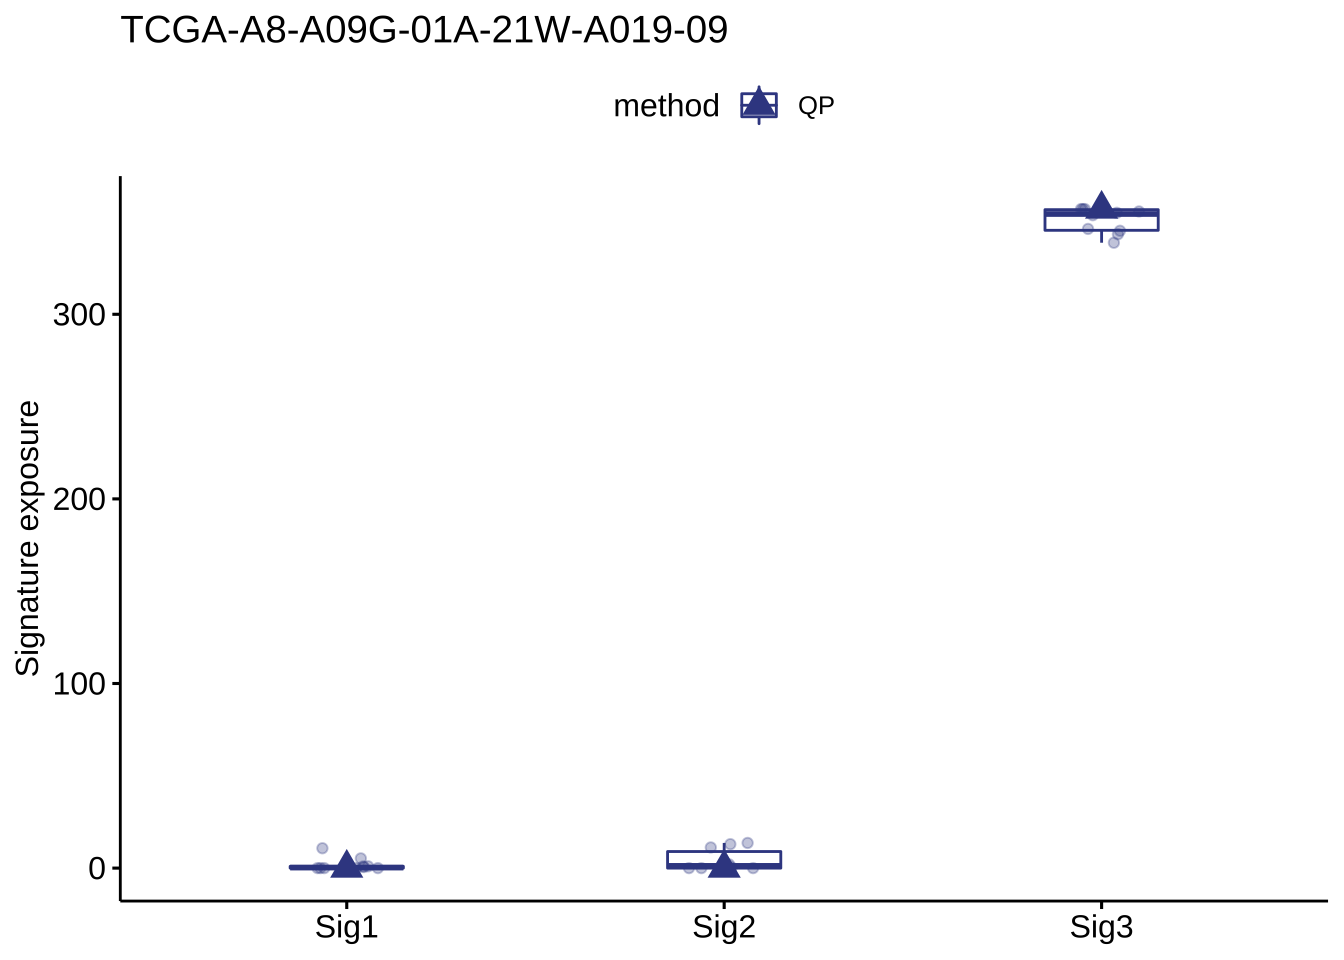
\includegraphics[width=0.95\linewidth]{sigminer_files/figure-latex/unnamed-chunk-57-1}

\begin{Shaded}
\begin{Highlighting}[]
\FunctionTok{show\_sig\_bootstrap\_error}\NormalTok{(bt\_result, }\AttributeTok{sample =} \StringTok{"TCGA{-}A8{-}A09G{-}01A{-}21W{-}A019{-}09"}\NormalTok{)}
\DocumentationTok{\#\# i [2022{-}08{-}29 11:08:19]: Started.}
\DocumentationTok{\#\# i [2022{-}08{-}29 11:08:19]: Plotting.}
\DocumentationTok{\#\# i [2022{-}08{-}29 11:08:19]: 0.05 secs elapsed.}
\end{Highlighting}
\end{Shaded}

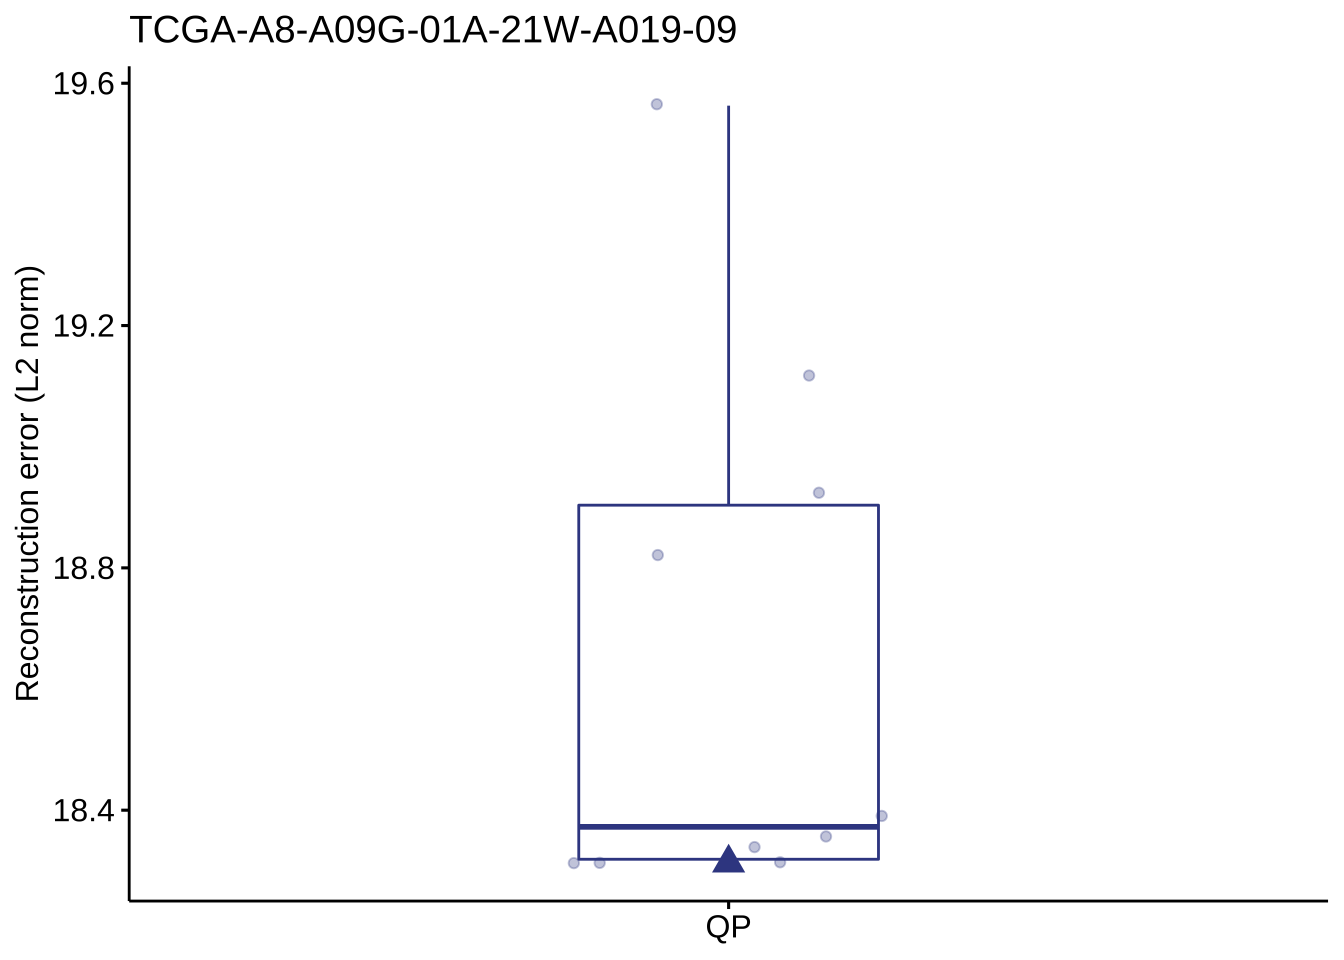
\includegraphics[width=0.95\linewidth]{sigminer_files/figure-latex/unnamed-chunk-58-1}

\begin{Shaded}
\begin{Highlighting}[]
\FunctionTok{show\_sig\_bootstrap\_stability}\NormalTok{(bt\_result)}
\DocumentationTok{\#\# i [2022{-}08{-}29 11:08:19]: Started.}
\DocumentationTok{\#\# i [2022{-}08{-}29 11:08:19]: Plotting.}
\DocumentationTok{\#\# i [2022{-}08{-}29 11:08:19]: 0.078 secs elapsed.}
\end{Highlighting}
\end{Shaded}

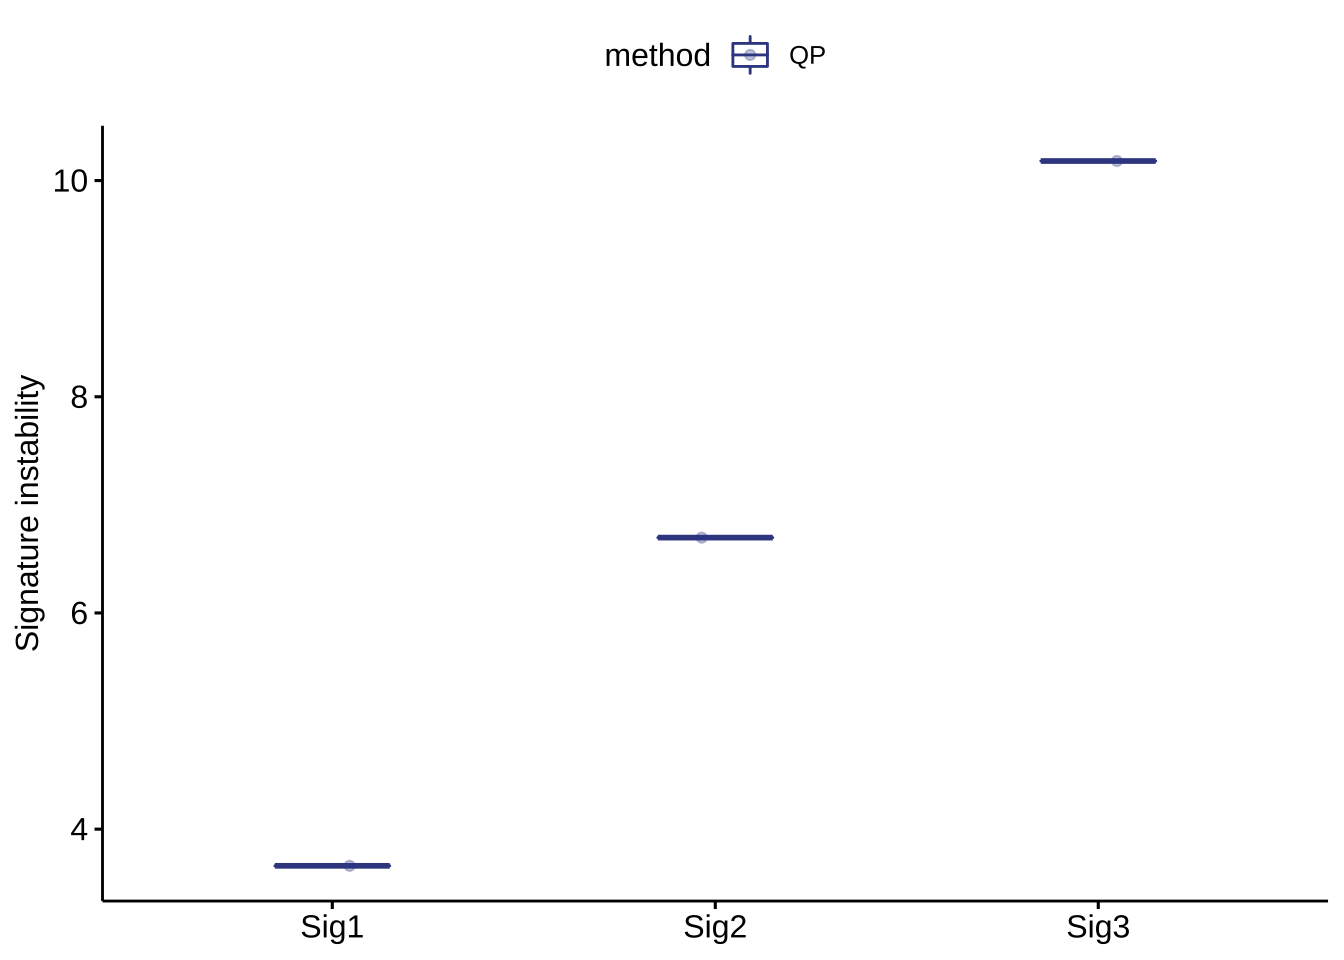
\includegraphics[width=0.95\linewidth]{sigminer_files/figure-latex/unnamed-chunk-59-1}

P values have been calculated under specified relative exposure cutoff (0.05 at default).

\hypertarget{analysis-supps}{%
\chapter{Other signature types}\label{analysis-supps}}

\hypertarget{copy-number-signature-wang-et-al}{%
\section{\texorpdfstring{Copy number signature (\emph{Wang} et al)}{Copy number signature (Wang et al)}}\label{copy-number-signature-wang-et-al}}

\hypertarget{read-data}{%
\subsection{Read data}\label{read-data}}

The input requires absolute copy number profile with following information:

\begin{itemize}
\tightlist
\item
  Segment chromosome.
\item
  Segment start.
\item
  Segment end.
\item
  \textbf{Absolute copy number value for this segment}: must be integer.
\item
  Sample ID.
\end{itemize}

The input data can be result from any software which provides information above.

Useful softwares are listed below:

\begin{itemize}
\tightlist
\item
  \href{https://software.broadinstitute.org/cancer/cga/absolute}{ABSOLUTE}.
\item
  \href{https://cran.r-project.org/web/packages/sequenza/index.html}{Sequenza}
\item
  \href{https://github.com/mskcc/facets}{FACETS}
\item
  \href{http://penncnv.openbioinformatics.org/en/latest/}{PennCNV} \& \href{https://www.crick.ac.uk/research/labs/peter-van-loo/software}{ASCAT}
\item
  \href{https://github.com/etal/cnvkit}{CNVkit}
\end{itemize}

Useful analysis reference:

\begin{itemize}
\tightlist
\item
  \href{https://xsliulab.github.io/PC_CNA_signature/}{Prostate Cancer Variation Signature Analysis Report}
\end{itemize}

The import work is done by \texttt{read\_copynumber()}, which supports \texttt{data.frame} or file, and even result directory from \textbf{ABSOLUTE}.

Option \texttt{sigminer.sex} is used to control the processing of sex. If you don't care the sex chromosomes (i.e.~X and Y),
you can ignore this setting after removing the X/Y segments, otherwise the \texttt{summary} in the result \texttt{cn} and tally process may be biased.

\begin{Shaded}
\begin{Highlighting}[]
\DocumentationTok{\#\# Default is "female"}
\DocumentationTok{\#\# You can ignore the setting if all samples are females}
\DocumentationTok{\#\# But we recommend you set it}
\FunctionTok{options}\NormalTok{(}\AttributeTok{sigminer.sex =} \StringTok{"male"}\NormalTok{)}
\DocumentationTok{\#\# For cohort contains both males and females,}
\DocumentationTok{\#\# set a data.frame with two columns, i.e.}
\DocumentationTok{\#\# options(sigminer.sex = sex\_df),}
\DocumentationTok{\#\# which}
\DocumentationTok{\#\# sex\_df = data.frame(sample = c("sample1", "sample2",}
\DocumentationTok{\#\#                     sex = "female", "male"))}
\CommentTok{\# Load toy dataset of absolute copynumber profile}
\FunctionTok{load}\NormalTok{(}\FunctionTok{system.file}\NormalTok{(}\StringTok{"extdata"}\NormalTok{, }\StringTok{"toy\_segTab.RData"}\NormalTok{,}
  \AttributeTok{package =} \StringTok{"sigminer"}\NormalTok{, }\AttributeTok{mustWork =} \ConstantTok{TRUE}
\NormalTok{))}
\NormalTok{cn }\OtherTok{\textless{}{-}} \FunctionTok{read\_copynumber}\NormalTok{(segTabs,}
  \AttributeTok{seg\_cols =} \FunctionTok{c}\NormalTok{(}\StringTok{"chromosome"}\NormalTok{, }\StringTok{"start"}\NormalTok{, }\StringTok{"end"}\NormalTok{, }\StringTok{"segVal"}\NormalTok{),}
  \AttributeTok{genome\_build =} \StringTok{"hg19"}\NormalTok{, }\AttributeTok{complement =} \ConstantTok{FALSE}\NormalTok{, }\AttributeTok{verbose =} \ConstantTok{TRUE}
\NormalTok{)}
\DocumentationTok{\#\# i [2022{-}08{-}29 11:08:20]: Started.}
\DocumentationTok{\#\# i [2022{-}08{-}29 11:08:20]: Genome build  : hg19.}
\DocumentationTok{\#\# i [2022{-}08{-}29 11:08:20]: Genome measure: called.}
\DocumentationTok{\#\# v [2022{-}08{-}29 11:08:20]: Chromosome size database for build obtained.}
\DocumentationTok{\#\# i [2022{-}08{-}29 11:08:20]: Reading input.}
\DocumentationTok{\#\# v [2022{-}08{-}29 11:08:20]: A data frame as input detected.}
\DocumentationTok{\#\# v [2022{-}08{-}29 11:08:20]: Column names checked.}
\DocumentationTok{\#\# v [2022{-}08{-}29 11:08:20]: Column order set.}
\DocumentationTok{\#\# v [2022{-}08{-}29 11:08:20]: Chromosomes unified.}
\DocumentationTok{\#\# v [2022{-}08{-}29 11:08:20]: Data imported.}
\DocumentationTok{\#\# i [2022{-}08{-}29 11:08:20]: Segments info:}
\DocumentationTok{\#\# i [2022{-}08{-}29 11:08:20]:     Keep {-} 467}
\DocumentationTok{\#\# i [2022{-}08{-}29 11:08:20]:     Drop {-} 0}
\DocumentationTok{\#\# v [2022{-}08{-}29 11:08:20]: Segments sorted.}
\DocumentationTok{\#\# i [2022{-}08{-}29 11:08:20]: Joining adjacent segments with same copy number value. Be patient...}
\DocumentationTok{\#\# v [2022{-}08{-}29 11:08:20]: 400 segments left after joining.}
\DocumentationTok{\#\# v [2022{-}08{-}29 11:08:20]: Segmental table cleaned.}
\DocumentationTok{\#\# i [2022{-}08{-}29 11:08:20]: Annotating.}
\DocumentationTok{\#\# v [2022{-}08{-}29 11:08:20]: Annotation done.}
\DocumentationTok{\#\# i [2022{-}08{-}29 11:08:20]: Summarizing per sample.}
\DocumentationTok{\#\# v [2022{-}08{-}29 11:08:20]: Summarized.}
\DocumentationTok{\#\# i [2022{-}08{-}29 11:08:20]: Generating CopyNumber object.}
\DocumentationTok{\#\# v [2022{-}08{-}29 11:08:20]: Generated.}
\DocumentationTok{\#\# i [2022{-}08{-}29 11:08:20]: Validating object.}
\DocumentationTok{\#\# v [2022{-}08{-}29 11:08:20]: Done.}
\DocumentationTok{\#\# i [2022{-}08{-}29 11:08:20]: 0.277 secs elapsed.}
\NormalTok{cn}
\DocumentationTok{\#\# An object of class CopyNumber }
\DocumentationTok{\#\# =============================}
\DocumentationTok{\#\#                           sample n\_of\_seg n\_of\_cnv n\_of\_amp n\_of\_del n\_of\_vchr}
\DocumentationTok{\#\#  1: TCGA{-}DF{-}A2KN{-}01A{-}11D{-}A17U{-}01       33        6        5        1         4}
\DocumentationTok{\#\#  2: TCGA{-}19{-}2621{-}01B{-}01D{-}0911{-}01       33        8        5        3         5}
\DocumentationTok{\#\#  3: TCGA{-}B6{-}A0X5{-}01A{-}21D{-}A107{-}01       28        8        4        4         2}
\DocumentationTok{\#\#  4: TCGA{-}A8{-}A07S{-}01A{-}11D{-}A036{-}01       38       11        2        9         4}
\DocumentationTok{\#\#  5: TCGA{-}26{-}6174{-}01A{-}21D{-}1842{-}01       43       13        8        5         8}
\DocumentationTok{\#\#  6: TCGA{-}CV{-}7432{-}01A{-}11D{-}2128{-}01       40       16        7        9         9}
\DocumentationTok{\#\#  7: TCGA{-}06{-}0644{-}01A{-}02D{-}0310{-}01       46       19        5       14         8}
\DocumentationTok{\#\#  8: TCGA{-}A5{-}A0G2{-}01A{-}11D{-}A042{-}01       39       21        5       16        10}
\DocumentationTok{\#\#  9: TCGA{-}99{-}7458{-}01A{-}11D{-}2035{-}01       48       26       10       16        13}
\DocumentationTok{\#\# 10: TCGA{-}05{-}4417{-}01A{-}22D{-}1854{-}01       52       37       33        4        17}
\DocumentationTok{\#\#     cna\_burden}
\DocumentationTok{\#\#  1:      0.000}
\DocumentationTok{\#\#  2:      0.099}
\DocumentationTok{\#\#  3:      0.087}
\DocumentationTok{\#\#  4:      0.112}
\DocumentationTok{\#\#  5:      0.119}
\DocumentationTok{\#\#  6:      0.198}
\DocumentationTok{\#\#  7:      0.165}
\DocumentationTok{\#\#  8:      0.393}
\DocumentationTok{\#\#  9:      0.318}
\DocumentationTok{\#\# 10:      0.654}
\end{Highlighting}
\end{Shaded}

\begin{quote}
Currently, you can refer to \texttt{extract\_facets\_cnv()} and \texttt{extract\_seqz\_cnv()} in \url{https://github.com/ShixiangWang/prad_signature/blob/master/analysis/src/99-functions.R} to
see how to get tidy data from a result directory of FACETS or Sequenza.
\#\# Tally Components
\end{quote}

Currently, there are two methods for generating sample-by-component matrix.

Option \texttt{sigminer.copynumber.max} is used to control the processing of max copy number values. Run \texttt{?sig\_tally} to see more.

\begin{Shaded}
\begin{Highlighting}[]
\DocumentationTok{\#\# Even you set max\_copynumber = 20 in read\_copynumber(),}
\DocumentationTok{\#\# the segmental copy number may be greater than 20}
\DocumentationTok{\#\# because for male samples, the X/Y segmental copy number}
\DocumentationTok{\#\# values will be doubled in tally process.}
\DocumentationTok{\#\# This setting will make copy number values of all segments}
\DocumentationTok{\#\# not greater than 20.}
\FunctionTok{options}\NormalTok{(}\AttributeTok{sigminer.copynumber.max =} \DecValTok{20}\NormalTok{)}
\CommentTok{\# Load copy number object}
\FunctionTok{load}\NormalTok{(}\FunctionTok{system.file}\NormalTok{(}\StringTok{"extdata"}\NormalTok{, }\StringTok{"toy\_copynumber.RData"}\NormalTok{,}
  \AttributeTok{package =} \StringTok{"sigminer"}\NormalTok{, }\AttributeTok{mustWork =} \ConstantTok{TRUE}
\NormalTok{))}
\CommentTok{\# Use method designed by Wang, Shixiang et al.}
\NormalTok{cn\_tally\_W }\OtherTok{\textless{}{-}} \FunctionTok{sig\_tally}\NormalTok{(cn, }\AttributeTok{method =} \StringTok{"W"}\NormalTok{)}
\end{Highlighting}
\end{Shaded}

\begin{quote}
You can set \texttt{options(sigminer.sex\ =\ "male",\ sigminer.copynumber.max\ =\ 20)} at the top of your code
to avoid setting them in two places.

\textbf{Of note}, the \texttt{sigminer.copynumber.max} option only has effect on \texttt{sig\_tally()} with method ``W'',
the \texttt{sigminer.sex} option has effects on \texttt{read\_copynumber()} and \texttt{sig\_tally()} with method ``W''.
\end{quote}

This step return a \texttt{list} containing information about copy number features, components and matrix for NMF etc.

\hypertarget{extract-signatures}{%
\subsection{Extract signatures}\label{extract-signatures}}

When you get the matrix, you can just do the signature extraction as SBS etc. signatures. So here we won't talk much.

\begin{Shaded}
\begin{Highlighting}[]
\NormalTok{cn\_tally\_W}\SpecialCharTok{$}\NormalTok{nmf\_matrix[}\DecValTok{1}\SpecialCharTok{:}\DecValTok{5}\NormalTok{, }\DecValTok{1}\SpecialCharTok{:}\DecValTok{5}\NormalTok{]}
\DocumentationTok{\#\#                              BP10MB[0] BP10MB[1] BP10MB[2] BP10MB[3] BP10MB[4]}
\DocumentationTok{\#\# TCGA{-}05{-}4417{-}01A{-}22D{-}1854{-}01       275        20         5         0         0}
\DocumentationTok{\#\# TCGA{-}06{-}0644{-}01A{-}02D{-}0310{-}01       289         5         4         0         1}
\DocumentationTok{\#\# TCGA{-}19{-}2621{-}01B{-}01D{-}0911{-}01       294         2         3         1         0}
\DocumentationTok{\#\# TCGA{-}26{-}6174{-}01A{-}21D{-}1842{-}01       288         4         7         1         0}
\DocumentationTok{\#\# TCGA{-}99{-}7458{-}01A{-}11D{-}2035{-}01       284         9         5         1         1}
\end{Highlighting}
\end{Shaded}

\begin{Shaded}
\begin{Highlighting}[]
\CommentTok{\# library(NMF)}
\NormalTok{sig\_w }\OtherTok{\textless{}{-}} \FunctionTok{sig\_extract}\NormalTok{(cn\_tally\_W}\SpecialCharTok{$}\NormalTok{nmf\_matrix, }\AttributeTok{n\_sig =} \DecValTok{2}\NormalTok{)}
\end{Highlighting}
\end{Shaded}

\hypertarget{allele-specific-copy-number-signature-steele-et-al}{%
\section{\texorpdfstring{Allele specific copy number signature (\emph{Steele} et al)}{Allele specific copy number signature (Steele et al)}}\label{allele-specific-copy-number-signature-steele-et-al}}

Previously described steps can be also applied to allele specific copy number
profile with \emph{Steele} et al approach. There are two catalog methods provided by
\emph{Steele} et al: 40 catalogs and 48 catalogs. In current stage, 48 catalog is
recommended as \textasciitilde20 reference signatures have been built on \textasciitilde10,000 TCGA tumors.
reference example is given below:

\begin{Shaded}
\begin{Highlighting}[]
\CommentTok{\# Generate example data}
\FunctionTok{load}\NormalTok{(}\FunctionTok{system.file}\NormalTok{(}\StringTok{"extdata"}\NormalTok{, }\StringTok{"toy\_segTab.RData"}\NormalTok{,}
  \AttributeTok{package =} \StringTok{"sigminer"}\NormalTok{, }\AttributeTok{mustWork =} \ConstantTok{TRUE}
\NormalTok{))}
\FunctionTok{set.seed}\NormalTok{(}\DecValTok{1234}\NormalTok{)}
\CommentTok{\# Make sure minor\_cn is provided}
\NormalTok{segTabs}\SpecialCharTok{$}\NormalTok{minor\_cn }\OtherTok{\textless{}{-}} \FunctionTok{sample}\NormalTok{(}\FunctionTok{c}\NormalTok{(}\DecValTok{0}\NormalTok{, }\DecValTok{1}\NormalTok{), }\AttributeTok{size =} \FunctionTok{nrow}\NormalTok{(segTabs), }\AttributeTok{replace =} \ConstantTok{TRUE}\NormalTok{)}
\NormalTok{cn2 }\OtherTok{\textless{}{-}} \FunctionTok{read\_copynumber}\NormalTok{(segTabs,}
  \AttributeTok{seg\_cols =} \FunctionTok{c}\NormalTok{(}\StringTok{"chromosome"}\NormalTok{, }\StringTok{"start"}\NormalTok{, }\StringTok{"end"}\NormalTok{, }\StringTok{"segVal"}\NormalTok{),}
  \AttributeTok{genome\_measure =} \StringTok{"wg"}\NormalTok{, }\AttributeTok{complement =} \ConstantTok{TRUE}\NormalTok{, }\AttributeTok{add\_loh =} \ConstantTok{TRUE}
\NormalTok{)}
\DocumentationTok{\#\# i [2022{-}08{-}29 11:25:42]: Started.}
\DocumentationTok{\#\# i [2022{-}08{-}29 11:25:42]: Genome build  : hg19.}
\DocumentationTok{\#\# i [2022{-}08{-}29 11:25:42]: Genome measure: wg.}
\DocumentationTok{\#\# i [2022{-}08{-}29 11:25:42]: When add\_loh is TRUE, use\_all is forced to TRUE.}
\DocumentationTok{\#\# Please drop columns you don\textquotesingle{}t want to keep before reading.}
\DocumentationTok{\#\# v [2022{-}08{-}29 11:25:42]: Chromosome size database for build obtained.}
\DocumentationTok{\#\# i [2022{-}08{-}29 11:25:42]: Reading input.}
\DocumentationTok{\#\# v [2022{-}08{-}29 11:25:42]: A data frame as input detected.}
\DocumentationTok{\#\# v [2022{-}08{-}29 11:25:42]: Column names checked.}
\DocumentationTok{\#\# v [2022{-}08{-}29 11:25:42]: Column order set.}
\DocumentationTok{\#\# v [2022{-}08{-}29 11:25:42]: Chromosomes unified.}
\DocumentationTok{\#\# v [2022{-}08{-}29 11:25:42]: Value 2 (normal copy) filled to uncalled chromosomes.}
\DocumentationTok{\#\# v [2022{-}08{-}29 11:25:42]: Data imported.}
\DocumentationTok{\#\# i [2022{-}08{-}29 11:25:42]: Segments info:}
\DocumentationTok{\#\# i [2022{-}08{-}29 11:25:42]:     Keep {-} 477}
\DocumentationTok{\#\# i [2022{-}08{-}29 11:25:42]:     Drop {-} 0}
\DocumentationTok{\#\# v [2022{-}08{-}29 11:25:42]: Segments sorted.}
\DocumentationTok{\#\# i [2022{-}08{-}29 11:25:43]: Adding LOH labels...}
\DocumentationTok{\#\# i [2022{-}08{-}29 11:25:43]: Joining adjacent segments with same copy number value. Be patient...}
\DocumentationTok{\#\# v [2022{-}08{-}29 11:25:43]: 410 segments left after joining.}
\DocumentationTok{\#\# v [2022{-}08{-}29 11:25:43]: Segmental table cleaned.}
\DocumentationTok{\#\# i [2022{-}08{-}29 11:25:43]: Annotating.}
\DocumentationTok{\#\# v [2022{-}08{-}29 11:25:43]: Annotation done.}
\DocumentationTok{\#\# i [2022{-}08{-}29 11:25:43]: Summarizing per sample.}
\DocumentationTok{\#\# v [2022{-}08{-}29 11:25:43]: Summarized.}
\DocumentationTok{\#\# i [2022{-}08{-}29 11:25:43]: Generating CopyNumber object.}
\DocumentationTok{\#\# v [2022{-}08{-}29 11:25:43]: Generated.}
\DocumentationTok{\#\# i [2022{-}08{-}29 11:25:43]: Validating object.}
\DocumentationTok{\#\# v [2022{-}08{-}29 11:25:43]: Done.}
\DocumentationTok{\#\# i [2022{-}08{-}29 11:25:43]: 0.616 secs elapsed.}

\CommentTok{\# Use tally method "S" (Steele et al.)}
\NormalTok{tally\_s2 }\OtherTok{\textless{}{-}} \FunctionTok{sig\_tally}\NormalTok{(cn2, }\AttributeTok{method =} \StringTok{"S"}\NormalTok{)}
\DocumentationTok{\#\# i [2022{-}08{-}29 11:25:43]: Started.}
\DocumentationTok{\#\# i [2022{-}08{-}29 11:25:43]: When you use method \textquotesingle{}S\textquotesingle{}, please make sure you have set \textquotesingle{}join\_adj\_seg\textquotesingle{} to FALSE and \textquotesingle{}add\_loh\textquotesingle{} to TRUE in \textquotesingle{}read\_copynumber() in the previous step!}
\DocumentationTok{\#\# v [2022{-}08{-}29 11:25:43]: Matrix generated.}
\DocumentationTok{\#\# i [2022{-}08{-}29 11:25:43]: 0.052 secs elapsed.}

\NormalTok{cn\_sig2 }\OtherTok{\textless{}{-}} \FunctionTok{sig\_extract}\NormalTok{(tally\_s2}\SpecialCharTok{$}\NormalTok{all\_matrices}\SpecialCharTok{$}\NormalTok{CN\_48, }\AttributeTok{n\_sig =} \DecValTok{2}\NormalTok{)}
\DocumentationTok{\#\# NMF algorithm: \textquotesingle{}brunet\textquotesingle{}}
\DocumentationTok{\#\# Multiple runs: 10}
\DocumentationTok{\#\# Mode: sequential [foreach:doParallelMC]}
\DocumentationTok{\#\# Runs: |                                                        Runs: |                                                  |   0\%Runs: |                                                        Runs: |=====                                             |   9\%Runs: |                                                        Runs: |=========                                         |  18\%Runs: |                                                        Runs: |==============                                    |  27\%Runs: |                                                        Runs: |==================                                |  36\%Runs: |                                                        Runs: |=======================                           |  45\%Runs: |                                                        Runs: |===========================                       |  55\%Runs: |                                                        Runs: |================================                  |  64\%Runs: |                                                        Runs: |====================================              |  73\%Runs: |                                                        Runs: |=========================================         |  82\%Runs: |                                                        Runs: |=============================================     |  91\%Runs: |                                                        Runs: |==================================================| 100\%}
\DocumentationTok{\#\# System time:}
\DocumentationTok{\#\#    user  system elapsed }
\DocumentationTok{\#\#   9.635   0.175   9.917}
\FunctionTok{get\_sig\_similarity}\NormalTok{(cn\_sig2, }\AttributeTok{sig\_db =} \StringTok{"CNS\_TCGA"}\NormalTok{)}
\DocumentationTok{\#\# {-}Comparing against COSMIC signatures}
\DocumentationTok{\#\# {-}{-}{-}{-}{-}{-}{-}{-}{-}{-}{-}{-}{-}{-}{-}{-}{-}{-}{-}{-}{-}{-}{-}{-}{-}{-}{-}{-}{-}{-}{-}{-}{-}{-}{-}{-}}
\DocumentationTok{\#\# {-}{-}Found Sig1 most similar to CN1}
\DocumentationTok{\#\#    Aetiology: See https://cancer.sanger.ac.uk/signatures/cn/ [similarity: 0.728]}
\DocumentationTok{\#\# {-}{-}Found Sig2 most similar to CN2}
\DocumentationTok{\#\#    Aetiology: See https://cancer.sanger.ac.uk/signatures/cn/ [similarity: 0.668]}
\DocumentationTok{\#\# {-}{-}{-}{-}{-}{-}{-}{-}{-}{-}{-}{-}{-}{-}{-}{-}{-}{-}{-}{-}{-}{-}{-}{-}{-}{-}{-}{-}{-}{-}{-}{-}{-}{-}{-}{-}}
\DocumentationTok{\#\# Return result invisiblely.}
\end{Highlighting}
\end{Shaded}

\hypertarget{rearrangement-signature}{%
\section{Rearrangement signature}\label{rearrangement-signature}}

Similarity, once you know how to generate matrix for genome rearrangement signature,
you can easily apply the signature extraction or signature fitting.

\begin{Shaded}
\begin{Highlighting}[]
\NormalTok{sv }\OtherTok{\textless{}{-}} \FunctionTok{readRDS}\NormalTok{(}\FunctionTok{system.file}\NormalTok{(}\StringTok{"extdata"}\NormalTok{, }\StringTok{"toy\_sv.rds"}\NormalTok{, }\AttributeTok{package =} \StringTok{"sigminer"}\NormalTok{, }\AttributeTok{mustWork =} \ConstantTok{TRUE}\NormalTok{))}
\NormalTok{rs }\OtherTok{\textless{}{-}} \FunctionTok{read\_sv\_as\_rs}\NormalTok{(sv)}
\DocumentationTok{\#\# succesfully read RS!}
\CommentTok{\# svclass is optional}
\NormalTok{rs2 }\OtherTok{\textless{}{-}} \FunctionTok{read\_sv\_as\_rs}\NormalTok{(sv[, }\FunctionTok{setdiff}\NormalTok{(}\FunctionTok{colnames}\NormalTok{(sv), }\StringTok{"svclass"}\NormalTok{)])}
\DocumentationTok{\#\# succesfully read RS!}
\FunctionTok{identical}\NormalTok{(rs, rs2)}
\DocumentationTok{\#\# [1] TRUE}

\NormalTok{tally\_rs }\OtherTok{\textless{}{-}} \FunctionTok{sig\_tally}\NormalTok{(rs)}
\DocumentationTok{\#\# i [2022{-}08{-}29 11:08:35]: Started.}
\DocumentationTok{\#\# v [2022{-}08{-}29 11:08:35]: Successfully get RS list!}
\DocumentationTok{\#\# }
\DocumentationTok{\#\# Attaching package: \textquotesingle{}purrr\textquotesingle{}}
\DocumentationTok{\#\# The following objects are masked from \textquotesingle{}package:foreach\textquotesingle{}:}
\DocumentationTok{\#\# }
\DocumentationTok{\#\#     accumulate, when}
\DocumentationTok{\#\# The following object is masked from \textquotesingle{}package:XVector\textquotesingle{}:}
\DocumentationTok{\#\# }
\DocumentationTok{\#\#     compact}
\DocumentationTok{\#\# The following object is masked from \textquotesingle{}package:GenomicRanges\textquotesingle{}:}
\DocumentationTok{\#\# }
\DocumentationTok{\#\#     reduce}
\DocumentationTok{\#\# The following object is masked from \textquotesingle{}package:IRanges\textquotesingle{}:}
\DocumentationTok{\#\# }
\DocumentationTok{\#\#     reduce}
\DocumentationTok{\#\# [1] "Getting clustered info..."}
\DocumentationTok{\#\# pcf finished for chromosome arm 1p }
\DocumentationTok{\#\# pcf finished for chromosome arm 10p }
\DocumentationTok{\#\# pcf finished for chromosome arm 10q }
\DocumentationTok{\#\# pcf finished for chromosome arm 11p }
\DocumentationTok{\#\# pcf finished for chromosome arm 11q }
\DocumentationTok{\#\# pcf finished for chromosome arm 12p }
\DocumentationTok{\#\# pcf finished for chromosome arm 12q }
\DocumentationTok{\#\# pcf finished for chromosome arm 13q }
\DocumentationTok{\#\# pcf finished for chromosome arm 14q }
\DocumentationTok{\#\# pcf finished for chromosome arm 16q }
\DocumentationTok{\#\# pcf finished for chromosome arm 17p }
\DocumentationTok{\#\# pcf finished for chromosome arm 17q }
\DocumentationTok{\#\# pcf finished for chromosome arm 18p }
\DocumentationTok{\#\# pcf finished for chromosome arm 18q }
\DocumentationTok{\#\# pcf finished for chromosome arm 19p }
\DocumentationTok{\#\# pcf finished for chromosome arm 19q }
\DocumentationTok{\#\# pcf finished for chromosome arm 2p }
\DocumentationTok{\#\# pcf finished for chromosome arm 2q }
\DocumentationTok{\#\# pcf finished for chromosome arm 20p }
\DocumentationTok{\#\# pcf finished for chromosome arm 20q }
\DocumentationTok{\#\# pcf finished for chromosome arm 22q }
\DocumentationTok{\#\# pcf finished for chromosome arm 3p }
\DocumentationTok{\#\# pcf finished for chromosome arm 3q }
\DocumentationTok{\#\# pcf finished for chromosome arm 4p }
\DocumentationTok{\#\# pcf finished for chromosome arm 4q }
\DocumentationTok{\#\# pcf finished for chromosome arm 5p }
\DocumentationTok{\#\# pcf finished for chromosome arm 5q }
\DocumentationTok{\#\# pcf finished for chromosome arm 6p }
\DocumentationTok{\#\# pcf finished for chromosome arm 6q }
\DocumentationTok{\#\# pcf finished for chromosome arm 7p }
\DocumentationTok{\#\# pcf finished for chromosome arm 7q }
\DocumentationTok{\#\# pcf finished for chromosome arm 8p }
\DocumentationTok{\#\# pcf finished for chromosome arm 8q }
\DocumentationTok{\#\# pcf finished for chromosome arm 9p }
\DocumentationTok{\#\# pcf finished for chromosome arm 9q }
\DocumentationTok{\#\# pcf finished for chromosome arm Xp }
\DocumentationTok{\#\# pcf finished for chromosome arm Xq }
\DocumentationTok{\#\# pcf finished for chromosome arm 21q }
\DocumentationTok{\#\# pcf finished for chromosome arm 1p }
\DocumentationTok{\#\# pcf finished for chromosome arm 1q }
\DocumentationTok{\#\# pcf finished for chromosome arm 10p }
\DocumentationTok{\#\# pcf finished for chromosome arm 10q }
\DocumentationTok{\#\# pcf finished for chromosome arm 11q }
\DocumentationTok{\#\# pcf finished for chromosome arm 12p }
\DocumentationTok{\#\# pcf finished for chromosome arm 12q }
\DocumentationTok{\#\# pcf finished for chromosome arm 13q }
\DocumentationTok{\#\# pcf finished for chromosome arm 14q }
\DocumentationTok{\#\# pcf finished for chromosome arm 15q }
\DocumentationTok{\#\# pcf finished for chromosome arm 16p }
\DocumentationTok{\#\# pcf finished for chromosome arm 16q }
\DocumentationTok{\#\# pcf finished for chromosome arm 17p }
\DocumentationTok{\#\# pcf finished for chromosome arm 17q }
\DocumentationTok{\#\# pcf finished for chromosome arm 18q }
\DocumentationTok{\#\# pcf finished for chromosome arm 19q }
\DocumentationTok{\#\# pcf finished for chromosome arm 2p }
\DocumentationTok{\#\# pcf finished for chromosome arm 2q }
\DocumentationTok{\#\# pcf finished for chromosome arm 20q }
\DocumentationTok{\#\# pcf finished for chromosome arm 21p }
\DocumentationTok{\#\# pcf finished for chromosome arm 21q }
\DocumentationTok{\#\# pcf finished for chromosome arm 22q }
\DocumentationTok{\#\# pcf finished for chromosome arm 3p }
\DocumentationTok{\#\# pcf finished for chromosome arm 3q }
\DocumentationTok{\#\# pcf finished for chromosome arm 4p }
\DocumentationTok{\#\# pcf finished for chromosome arm 4q }
\DocumentationTok{\#\# pcf finished for chromosome arm 5p }
\DocumentationTok{\#\# pcf finished for chromosome arm 5q }
\DocumentationTok{\#\# pcf finished for chromosome arm 6p }
\DocumentationTok{\#\# pcf finished for chromosome arm 7q }
\DocumentationTok{\#\# pcf finished for chromosome arm 8p }
\DocumentationTok{\#\# pcf finished for chromosome arm 8q }
\DocumentationTok{\#\# pcf finished for chromosome arm 9p }
\DocumentationTok{\#\# pcf finished for chromosome arm 9q }
\DocumentationTok{\#\# pcf finished for chromosome arm Xp }
\DocumentationTok{\#\# pcf finished for chromosome arm Xq }
\DocumentationTok{\#\# pcf finished for chromosome arm 1p }
\DocumentationTok{\#\# pcf finished for chromosome arm 1q }
\DocumentationTok{\#\# pcf finished for chromosome arm 10q }
\DocumentationTok{\#\# pcf finished for chromosome arm 11p }
\DocumentationTok{\#\# pcf finished for chromosome arm 11q }
\DocumentationTok{\#\# pcf finished for chromosome arm 12p }
\DocumentationTok{\#\# pcf finished for chromosome arm 13q }
\DocumentationTok{\#\# pcf finished for chromosome arm 14q }
\DocumentationTok{\#\# pcf finished for chromosome arm 15q }
\DocumentationTok{\#\# pcf finished for chromosome arm 16p }
\DocumentationTok{\#\# pcf finished for chromosome arm 17p }
\DocumentationTok{\#\# pcf finished for chromosome arm 17q }
\DocumentationTok{\#\# pcf finished for chromosome arm 18p }
\DocumentationTok{\#\# pcf finished for chromosome arm 18q }
\DocumentationTok{\#\# pcf finished for chromosome arm 19p }
\DocumentationTok{\#\# pcf finished for chromosome arm 19q }
\DocumentationTok{\#\# pcf finished for chromosome arm 2p }
\DocumentationTok{\#\# pcf finished for chromosome arm 2q }
\DocumentationTok{\#\# pcf finished for chromosome arm 20p }
\DocumentationTok{\#\# pcf finished for chromosome arm 20q }
\DocumentationTok{\#\# pcf finished for chromosome arm 21q }
\DocumentationTok{\#\# pcf finished for chromosome arm 3p }
\DocumentationTok{\#\# pcf finished for chromosome arm 3q }
\DocumentationTok{\#\# pcf finished for chromosome arm 4p }
\DocumentationTok{\#\# pcf finished for chromosome arm 5q }
\DocumentationTok{\#\# pcf finished for chromosome arm 6p }
\DocumentationTok{\#\# pcf finished for chromosome arm 6q }
\DocumentationTok{\#\# pcf finished for chromosome arm 7q }
\DocumentationTok{\#\# pcf finished for chromosome arm 8p }
\DocumentationTok{\#\# pcf finished for chromosome arm 8q }
\DocumentationTok{\#\# pcf finished for chromosome arm 9p }
\DocumentationTok{\#\# pcf finished for chromosome arm 9q }
\DocumentationTok{\#\# pcf finished for chromosome arm Xq }
\DocumentationTok{\#\# pcf finished for chromosome arm 22q }
\DocumentationTok{\#\# pcf finished for chromosome arm 1p }
\DocumentationTok{\#\# pcf finished for chromosome arm 1q }
\DocumentationTok{\#\# pcf finished for chromosome arm 10q }
\DocumentationTok{\#\# pcf finished for chromosome arm 11p }
\DocumentationTok{\#\# pcf finished for chromosome arm 11q }
\DocumentationTok{\#\# pcf finished for chromosome arm 12p }
\DocumentationTok{\#\# pcf finished for chromosome arm 12q }
\DocumentationTok{\#\# pcf finished for chromosome arm 14q }
\DocumentationTok{\#\# pcf finished for chromosome arm 15q }
\DocumentationTok{\#\# pcf finished for chromosome arm 16p }
\DocumentationTok{\#\# pcf finished for chromosome arm 16q }
\DocumentationTok{\#\# pcf finished for chromosome arm 17p }
\DocumentationTok{\#\# pcf finished for chromosome arm 17q }
\DocumentationTok{\#\# pcf finished for chromosome arm 18q }
\DocumentationTok{\#\# pcf finished for chromosome arm 2p }
\DocumentationTok{\#\# pcf finished for chromosome arm 2q }
\DocumentationTok{\#\# pcf finished for chromosome arm 20p }
\DocumentationTok{\#\# pcf finished for chromosome arm 20q }
\DocumentationTok{\#\# pcf finished for chromosome arm 21q }
\DocumentationTok{\#\# pcf finished for chromosome arm 3p }
\DocumentationTok{\#\# pcf finished for chromosome arm 3q }
\DocumentationTok{\#\# pcf finished for chromosome arm 4p }
\DocumentationTok{\#\# pcf finished for chromosome arm 4q }
\DocumentationTok{\#\# pcf finished for chromosome arm 5p }
\DocumentationTok{\#\# pcf finished for chromosome arm 5q }
\DocumentationTok{\#\# pcf finished for chromosome arm 6p }
\DocumentationTok{\#\# pcf finished for chromosome arm 6q }
\DocumentationTok{\#\# pcf finished for chromosome arm 7p }
\DocumentationTok{\#\# pcf finished for chromosome arm 7q }
\DocumentationTok{\#\# pcf finished for chromosome arm 8p }
\DocumentationTok{\#\# pcf finished for chromosome arm 8q }
\DocumentationTok{\#\# pcf finished for chromosome arm 9p }
\DocumentationTok{\#\# pcf finished for chromosome arm 22q }
\DocumentationTok{\#\# pcf finished for chromosome arm Xq }
\DocumentationTok{\#\# pcf finished for chromosome arm 13q }
\DocumentationTok{\#\# pcf finished for chromosome arm 1p }
\DocumentationTok{\#\# pcf finished for chromosome arm 1q }
\DocumentationTok{\#\# pcf finished for chromosome arm 10p }
\DocumentationTok{\#\# pcf finished for chromosome arm 11p }
\DocumentationTok{\#\# pcf finished for chromosome arm 11q }
\DocumentationTok{\#\# pcf finished for chromosome arm 12p }
\DocumentationTok{\#\# pcf finished for chromosome arm 13q }
\DocumentationTok{\#\# pcf finished for chromosome arm 14q }
\DocumentationTok{\#\# pcf finished for chromosome arm 15q }
\DocumentationTok{\#\# pcf finished for chromosome arm 16q }
\DocumentationTok{\#\# pcf finished for chromosome arm 17p }
\DocumentationTok{\#\# pcf finished for chromosome arm 17q }
\DocumentationTok{\#\# pcf finished for chromosome arm 2p }
\DocumentationTok{\#\# pcf finished for chromosome arm 2q }
\DocumentationTok{\#\# pcf finished for chromosome arm 20q }
\DocumentationTok{\#\# pcf finished for chromosome arm 4q }
\DocumentationTok{\#\# pcf finished for chromosome arm 5p }
\DocumentationTok{\#\# pcf finished for chromosome arm 5q }
\DocumentationTok{\#\# pcf finished for chromosome arm 6p }
\DocumentationTok{\#\# pcf finished for chromosome arm 6q }
\DocumentationTok{\#\# pcf finished for chromosome arm 7p }
\DocumentationTok{\#\# pcf finished for chromosome arm 8p }
\DocumentationTok{\#\# pcf finished for chromosome arm 8q }
\DocumentationTok{\#\# pcf finished for chromosome arm 9q }
\DocumentationTok{\#\# pcf finished for chromosome arm Xp }
\DocumentationTok{\#\# pcf finished for chromosome arm Xq }
\DocumentationTok{\#\# pcf finished for chromosome arm 21p }
\DocumentationTok{\#\# pcf finished for chromosome arm 22q }
\DocumentationTok{\#\# pcf finished for chromosome arm 1p }
\DocumentationTok{\#\# pcf finished for chromosome arm 1q }
\DocumentationTok{\#\# pcf finished for chromosome arm 10p }
\DocumentationTok{\#\# pcf finished for chromosome arm 10q }
\DocumentationTok{\#\# pcf finished for chromosome arm 11p }
\DocumentationTok{\#\# pcf finished for chromosome arm 11q }
\DocumentationTok{\#\# pcf finished for chromosome arm 12p }
\DocumentationTok{\#\# pcf finished for chromosome arm 12q }
\DocumentationTok{\#\# pcf finished for chromosome arm 13q }
\DocumentationTok{\#\# pcf finished for chromosome arm 14q }
\DocumentationTok{\#\# pcf finished for chromosome arm 15q }
\DocumentationTok{\#\# pcf finished for chromosome arm 16p }
\DocumentationTok{\#\# pcf finished for chromosome arm 16q }
\DocumentationTok{\#\# pcf finished for chromosome arm 17p }
\DocumentationTok{\#\# pcf finished for chromosome arm 17q }
\DocumentationTok{\#\# pcf finished for chromosome arm 18p }
\DocumentationTok{\#\# pcf finished for chromosome arm 18q }
\DocumentationTok{\#\# pcf finished for chromosome arm 19p }
\DocumentationTok{\#\# pcf finished for chromosome arm 2p }
\DocumentationTok{\#\# pcf finished for chromosome arm 2q }
\DocumentationTok{\#\# pcf finished for chromosome arm 22q }
\DocumentationTok{\#\# pcf finished for chromosome arm 3p }
\DocumentationTok{\#\# pcf finished for chromosome arm 3q }
\DocumentationTok{\#\# pcf finished for chromosome arm 4p }
\DocumentationTok{\#\# pcf finished for chromosome arm 4q }
\DocumentationTok{\#\# pcf finished for chromosome arm 5p }
\DocumentationTok{\#\# pcf finished for chromosome arm 5q }
\DocumentationTok{\#\# pcf finished for chromosome arm 6p }
\DocumentationTok{\#\# pcf finished for chromosome arm 6q }
\DocumentationTok{\#\# pcf finished for chromosome arm 7p }
\DocumentationTok{\#\# pcf finished for chromosome arm 7q }
\DocumentationTok{\#\# pcf finished for chromosome arm 8p }
\DocumentationTok{\#\# pcf finished for chromosome arm 8q }
\DocumentationTok{\#\# pcf finished for chromosome arm 9p }
\DocumentationTok{\#\# pcf finished for chromosome arm 9q }
\DocumentationTok{\#\# pcf finished for chromosome arm Xp }
\DocumentationTok{\#\# pcf finished for chromosome arm Xq }
\DocumentationTok{\#\# pcf finished for chromosome arm 20q }
\DocumentationTok{\#\# pcf finished for chromosome arm 1p }
\DocumentationTok{\#\# pcf finished for chromosome arm 1q }
\DocumentationTok{\#\# pcf finished for chromosome arm 10p }
\DocumentationTok{\#\# pcf finished for chromosome arm 10q }
\DocumentationTok{\#\# pcf finished for chromosome arm 11p }
\DocumentationTok{\#\# pcf finished for chromosome arm 11q }
\DocumentationTok{\#\# pcf finished for chromosome arm 12p }
\DocumentationTok{\#\# pcf finished for chromosome arm 12q }
\DocumentationTok{\#\# pcf finished for chromosome arm 13q }
\DocumentationTok{\#\# pcf finished for chromosome arm 14q }
\DocumentationTok{\#\# pcf finished for chromosome arm 15q }
\DocumentationTok{\#\# pcf finished for chromosome arm 16p }
\DocumentationTok{\#\# pcf finished for chromosome arm 16q }
\DocumentationTok{\#\# pcf finished for chromosome arm 17p }
\DocumentationTok{\#\# pcf finished for chromosome arm 17q }
\DocumentationTok{\#\# pcf finished for chromosome arm 18q }
\DocumentationTok{\#\# pcf finished for chromosome arm 19p }
\DocumentationTok{\#\# pcf finished for chromosome arm 19q }
\DocumentationTok{\#\# pcf finished for chromosome arm 2p }
\DocumentationTok{\#\# pcf finished for chromosome arm 2q }
\DocumentationTok{\#\# pcf finished for chromosome arm 20p }
\DocumentationTok{\#\# pcf finished for chromosome arm 20q }
\DocumentationTok{\#\# pcf finished for chromosome arm 21q }
\DocumentationTok{\#\# pcf finished for chromosome arm 22q }
\DocumentationTok{\#\# pcf finished for chromosome arm 3p }
\DocumentationTok{\#\# pcf finished for chromosome arm 4p }
\DocumentationTok{\#\# pcf finished for chromosome arm 4q }
\DocumentationTok{\#\# pcf finished for chromosome arm 5p }
\DocumentationTok{\#\# pcf finished for chromosome arm 5q }
\DocumentationTok{\#\# pcf finished for chromosome arm 6p }
\DocumentationTok{\#\# pcf finished for chromosome arm 6q }
\DocumentationTok{\#\# pcf finished for chromosome arm 7p }
\DocumentationTok{\#\# pcf finished for chromosome arm 7q }
\DocumentationTok{\#\# pcf finished for chromosome arm 8p }
\DocumentationTok{\#\# pcf finished for chromosome arm 8q }
\DocumentationTok{\#\# pcf finished for chromosome arm 9p }
\DocumentationTok{\#\# pcf finished for chromosome arm 9q }
\DocumentationTok{\#\# pcf finished for chromosome arm Xp }
\DocumentationTok{\#\# pcf finished for chromosome arm Xq }
\DocumentationTok{\#\# pcf finished for chromosome arm Yq }
\DocumentationTok{\#\# pcf finished for chromosome arm 1p }
\DocumentationTok{\#\# pcf finished for chromosome arm 1q }
\DocumentationTok{\#\# pcf finished for chromosome arm 10p }
\DocumentationTok{\#\# pcf finished for chromosome arm 10q }
\DocumentationTok{\#\# pcf finished for chromosome arm 11p }
\DocumentationTok{\#\# pcf finished for chromosome arm 11q }
\DocumentationTok{\#\# pcf finished for chromosome arm 12p }
\DocumentationTok{\#\# pcf finished for chromosome arm 12q }
\DocumentationTok{\#\# pcf finished for chromosome arm 13q }
\DocumentationTok{\#\# pcf finished for chromosome arm 14q }
\DocumentationTok{\#\# pcf finished for chromosome arm 15q }
\DocumentationTok{\#\# pcf finished for chromosome arm 16p }
\DocumentationTok{\#\# pcf finished for chromosome arm 16q }
\DocumentationTok{\#\# pcf finished for chromosome arm 17p }
\DocumentationTok{\#\# pcf finished for chromosome arm 17q }
\DocumentationTok{\#\# pcf finished for chromosome arm 18p }
\DocumentationTok{\#\# pcf finished for chromosome arm 18q }
\DocumentationTok{\#\# pcf finished for chromosome arm 19p }
\DocumentationTok{\#\# pcf finished for chromosome arm 19q }
\DocumentationTok{\#\# pcf finished for chromosome arm 2p }
\DocumentationTok{\#\# pcf finished for chromosome arm 2q }
\DocumentationTok{\#\# pcf finished for chromosome arm 20p }
\DocumentationTok{\#\# pcf finished for chromosome arm 20q }
\DocumentationTok{\#\# pcf finished for chromosome arm 21q }
\DocumentationTok{\#\# pcf finished for chromosome arm 22q }
\DocumentationTok{\#\# pcf finished for chromosome arm 3p }
\DocumentationTok{\#\# pcf finished for chromosome arm 4p }
\DocumentationTok{\#\# pcf finished for chromosome arm 4q }
\DocumentationTok{\#\# pcf finished for chromosome arm 5p }
\DocumentationTok{\#\# pcf finished for chromosome arm 5q }
\DocumentationTok{\#\# pcf finished for chromosome arm 6p }
\DocumentationTok{\#\# pcf finished for chromosome arm 6q }
\DocumentationTok{\#\# pcf finished for chromosome arm 7p }
\DocumentationTok{\#\# pcf finished for chromosome arm 7q }
\DocumentationTok{\#\# pcf finished for chromosome arm 8p }
\DocumentationTok{\#\# pcf finished for chromosome arm 8q }
\DocumentationTok{\#\# pcf finished for chromosome arm 9p }
\DocumentationTok{\#\# pcf finished for chromosome arm 9q }
\DocumentationTok{\#\# pcf finished for chromosome arm Xp }
\DocumentationTok{\#\# pcf finished for chromosome arm Xq }
\DocumentationTok{\#\# pcf finished for chromosome arm 1p }
\DocumentationTok{\#\# pcf finished for chromosome arm 10q }
\DocumentationTok{\#\# pcf finished for chromosome arm 11q }
\DocumentationTok{\#\# pcf finished for chromosome arm 12p }
\DocumentationTok{\#\# pcf finished for chromosome arm 12q }
\DocumentationTok{\#\# pcf finished for chromosome arm 13q }
\DocumentationTok{\#\# pcf finished for chromosome arm 15q }
\DocumentationTok{\#\# pcf finished for chromosome arm 16q }
\DocumentationTok{\#\# pcf finished for chromosome arm 17p }
\DocumentationTok{\#\# pcf finished for chromosome arm 19p }
\DocumentationTok{\#\# pcf finished for chromosome arm 19q }
\DocumentationTok{\#\# pcf finished for chromosome arm 2p }
\DocumentationTok{\#\# pcf finished for chromosome arm 22q }
\DocumentationTok{\#\# pcf finished for chromosome arm 3q }
\DocumentationTok{\#\# pcf finished for chromosome arm 5p }
\DocumentationTok{\#\# pcf finished for chromosome arm 5q }
\DocumentationTok{\#\# pcf finished for chromosome arm 6q }
\DocumentationTok{\#\# pcf finished for chromosome arm 7p }
\DocumentationTok{\#\# pcf finished for chromosome arm 7q }
\DocumentationTok{\#\# pcf finished for chromosome arm 9p }
\DocumentationTok{\#\# pcf finished for chromosome arm 9q }
\DocumentationTok{\#\# pcf finished for chromosome arm Xq }
\DocumentationTok{\#\# pcf finished for chromosome arm 1p }
\DocumentationTok{\#\# pcf finished for chromosome arm 11q }
\DocumentationTok{\#\# pcf finished for chromosome arm 13q }
\DocumentationTok{\#\# pcf finished for chromosome arm 14q }
\DocumentationTok{\#\# pcf finished for chromosome arm 15q }
\DocumentationTok{\#\# pcf finished for chromosome arm 16p }
\DocumentationTok{\#\# pcf finished for chromosome arm 16q }
\DocumentationTok{\#\# pcf finished for chromosome arm 17p }
\DocumentationTok{\#\# pcf finished for chromosome arm 17q }
\DocumentationTok{\#\# pcf finished for chromosome arm 18p }
\DocumentationTok{\#\# pcf finished for chromosome arm 18q }
\DocumentationTok{\#\# pcf finished for chromosome arm 19p }
\DocumentationTok{\#\# pcf finished for chromosome arm 19q }
\DocumentationTok{\#\# pcf finished for chromosome arm 2p }
\DocumentationTok{\#\# pcf finished for chromosome arm 2q }
\DocumentationTok{\#\# pcf finished for chromosome arm 20p }
\DocumentationTok{\#\# pcf finished for chromosome arm 20q }
\DocumentationTok{\#\# pcf finished for chromosome arm 21p }
\DocumentationTok{\#\# pcf finished for chromosome arm 21q }
\DocumentationTok{\#\# pcf finished for chromosome arm 22q }
\DocumentationTok{\#\# pcf finished for chromosome arm 3p }
\DocumentationTok{\#\# pcf finished for chromosome arm 3q }
\DocumentationTok{\#\# pcf finished for chromosome arm 4p }
\DocumentationTok{\#\# pcf finished for chromosome arm 4q }
\DocumentationTok{\#\# pcf finished for chromosome arm 5p }
\DocumentationTok{\#\# pcf finished for chromosome arm 5q }
\DocumentationTok{\#\# pcf finished for chromosome arm 6p }
\DocumentationTok{\#\# pcf finished for chromosome arm 6q }
\DocumentationTok{\#\# pcf finished for chromosome arm 7p }
\DocumentationTok{\#\# pcf finished for chromosome arm 7q }
\DocumentationTok{\#\# pcf finished for chromosome arm 8p }
\DocumentationTok{\#\# pcf finished for chromosome arm 8q }
\DocumentationTok{\#\# pcf finished for chromosome arm 9p }
\DocumentationTok{\#\# pcf finished for chromosome arm 9q }
\DocumentationTok{\#\# pcf finished for chromosome arm Xp }
\DocumentationTok{\#\# pcf finished for chromosome arm Xq }
\DocumentationTok{\#\# pcf finished for chromosome arm Yp }
\DocumentationTok{\#\# pcf finished for chromosome arm Yq }
\DocumentationTok{\#\# [1] "Getting type of segment ..."}
\DocumentationTok{\#\# [1] "Getting distance of two rearrange segments ..."}
\DocumentationTok{\#\# v [2022{-}08{-}29 11:08:39]: Successfully get RS features!}
\DocumentationTok{\#\# v [2022{-}08{-}29 11:08:39]: Successfully get RS component!}
\DocumentationTok{\#\# v [2022{-}08{-}29 11:08:39]: Successfully get RS matrix!}
\DocumentationTok{\#\# i [2022{-}08{-}29 11:08:39]: 3.955 secs elapsed.}
\FunctionTok{str}\NormalTok{(tally\_rs)}
\DocumentationTok{\#\# List of 4}
\DocumentationTok{\#\#  $ features    :List of 3}
\DocumentationTok{\#\#   ..$ clustered:Classes \textquotesingle{}data.table\textquotesingle{} and \textquotesingle{}data.frame\textquotesingle{}:   4220 obs. of  3 variables:}
\DocumentationTok{\#\#   .. ..$ sample: chr [1:4220] "PD26861a" "PD26861a" "PD26861a" "PD26861a" ...}
\DocumentationTok{\#\#   .. ..$ value : chr [1:4220] "non{-}clustered" "non{-}clustered" "non{-}clustered" "non{-}clustered" ...}
\DocumentationTok{\#\#   .. ..$ Index : int [1:4220] 1 2 3 4 5 6 7 8 9 10 ...}
\DocumentationTok{\#\#   .. ..{-} attr(*, ".internal.selfref")=\textless{}externalptr\textgreater{} }
\DocumentationTok{\#\#   ..$ type     :Classes \textquotesingle{}data.table\textquotesingle{} and \textquotesingle{}data.frame\textquotesingle{}:   4220 obs. of  3 variables:}
\DocumentationTok{\#\#   .. ..$ sample: chr [1:4220] "PD26861a" "PD26861a" "PD26861a" "PD26861a" ...}
\DocumentationTok{\#\#   .. ..$ value : chr [1:4220] "inv" "inv" "del" "del" ...}
\DocumentationTok{\#\#   .. ..$ Index : int [1:4220] 1 2 3 4 5 6 7 8 9 10 ...}
\DocumentationTok{\#\#   .. ..{-} attr(*, ".internal.selfref")=\textless{}externalptr\textgreater{} }
\DocumentationTok{\#\#   ..$ size     :Classes \textquotesingle{}data.table\textquotesingle{} and \textquotesingle{}data.frame\textquotesingle{}:   4220 obs. of  3 variables:}
\DocumentationTok{\#\#   .. ..$ sample: chr [1:4220] "PD26861a" "PD26861a" "PD26861a" "PD26861a" ...}
\DocumentationTok{\#\#   .. ..$ value : chr [1:4220] "\textgreater{}10Mb" "1Mb{-}10Mb" "\textgreater{}10Mb" "100Kb{-}1Mb" ...}
\DocumentationTok{\#\#   .. ..$ Index : int [1:4220] 1 2 3 4 5 6 7 8 9 10 ...}
\DocumentationTok{\#\#   .. ..{-} attr(*, ".internal.selfref")=\textless{}externalptr\textgreater{} }
\DocumentationTok{\#\#  $ components  :List of 3}
\DocumentationTok{\#\#   ..$ clustered:Classes \textquotesingle{}data.table\textquotesingle{} and \textquotesingle{}data.frame\textquotesingle{}:   4220 obs. of  3 variables:}
\DocumentationTok{\#\#   .. ..$ sample     : chr [1:4220] "PD26861a" "PD26861a" "PD26861a" "PD26861a" ...}
\DocumentationTok{\#\#   .. ..$ Index      : int [1:4220] 1 2 3 4 5 6 7 8 9 10 ...}
\DocumentationTok{\#\#   .. ..$ C\_clustered: Factor w/ 2 levels "clustered","non{-}clustered": 2 2 2 2 2 2 2 2 2 2 ...}
\DocumentationTok{\#\#   .. ..{-} attr(*, ".internal.selfref")=\textless{}externalptr\textgreater{} }
\DocumentationTok{\#\#   ..$ type     :Classes \textquotesingle{}data.table\textquotesingle{} and \textquotesingle{}data.frame\textquotesingle{}:   4220 obs. of  3 variables:}
\DocumentationTok{\#\#   .. ..$ sample: chr [1:4220] "PD26861a" "PD26861a" "PD26861a" "PD26861a" ...}
\DocumentationTok{\#\#   .. ..$ Index : int [1:4220] 1 2 3 4 5 6 7 8 9 10 ...}
\DocumentationTok{\#\#   .. ..$ C\_type: Factor w/ 4 levels "del","inv","tds",..: 2 2 1 1 2 2 1 1 2 3 ...}
\DocumentationTok{\#\#   .. ..{-} attr(*, ".internal.selfref")=\textless{}externalptr\textgreater{} }
\DocumentationTok{\#\#   ..$ size     :Classes \textquotesingle{}data.table\textquotesingle{} and \textquotesingle{}data.frame\textquotesingle{}:   4220 obs. of  3 variables:}
\DocumentationTok{\#\#   .. ..$ sample: chr [1:4220] "PD26861a" "PD26861a" "PD26861a" "PD26861a" ...}
\DocumentationTok{\#\#   .. ..$ Index : int [1:4220] 1 2 3 4 5 6 7 8 9 10 ...}
\DocumentationTok{\#\#   .. ..$ C\_size: Factor w/ 6 levels "\textless{}1Kb","\textgreater{}10Mb",..: 2 6 2 5 2 2 6 5 5 5 ...}
\DocumentationTok{\#\#   .. ..{-} attr(*, ".internal.selfref")=\textless{}externalptr\textgreater{} }
\DocumentationTok{\#\#  $ nmf\_matrix  : int [1:10, 1:32] 13 3 2 0 1 3 2 11 5 1 ...}
\DocumentationTok{\#\#   ..{-} attr(*, "dimnames")=List of 2}
\DocumentationTok{\#\#   .. ..$ : chr [1:10] "PD26861a" "PD26862a" "PD26864a" "PD26865a" ...}
\DocumentationTok{\#\#   .. ..$ : chr [1:32] "clustered:del:\textgreater{}10Mb" "clustered:del:1{-}10Kb" "clustered:del:10{-}100Kb" "clustered:del:100Kb{-}1Mb" ...}
\DocumentationTok{\#\#  $ all\_matrices:List of 2}
\DocumentationTok{\#\#   ..$ RS\_32: int [1:10, 1:32] 13 3 2 0 1 3 2 11 5 1 ...}
\DocumentationTok{\#\#   .. ..{-} attr(*, "dimnames")=List of 2}
\DocumentationTok{\#\#   .. .. ..$ : chr [1:10] "PD26861a" "PD26862a" "PD26864a" "PD26865a" ...}
\DocumentationTok{\#\#   .. .. ..$ : chr [1:32] "clustered:del:\textgreater{}10Mb" "clustered:del:1{-}10Kb" "clustered:del:10{-}100Kb" "clustered:del:100Kb{-}1Mb" ...}
\DocumentationTok{\#\#   ..$ RS\_38: int [1:10, 1:38] 0 0 0 0 0 0 0 0 0 0 ...}
\DocumentationTok{\#\#   .. ..{-} attr(*, "dimnames")=List of 2}
\DocumentationTok{\#\#   .. .. ..$ : chr [1:10] "PD26861a" "PD26862a" "PD26864a" "PD26865a" ...}
\DocumentationTok{\#\#   .. .. ..$ : chr [1:38] "clustered:del:\textless{}1Kb" "clustered:del:\textgreater{}10Mb" "clustered:del:1{-}10Kb" "clustered:del:10{-}100Kb" ...}
\end{Highlighting}
\end{Shaded}

\hypertarget{target-vis}{%
\chapter{Target visualization}\label{target-vis}}

\hypertarget{copynumber-object}{%
\section{\texorpdfstring{\texttt{CopyNumber} object}{CopyNumber object}}\label{copynumber-object}}

\hypertarget{profile}{%
\subsection{Profile}\label{profile}}

\begin{Shaded}
\begin{Highlighting}[]
\FunctionTok{show\_cn\_profile}\NormalTok{(cn, }\AttributeTok{nrow =} \DecValTok{2}\NormalTok{, }\AttributeTok{ncol =} \DecValTok{1}\NormalTok{)}
\end{Highlighting}
\end{Shaded}

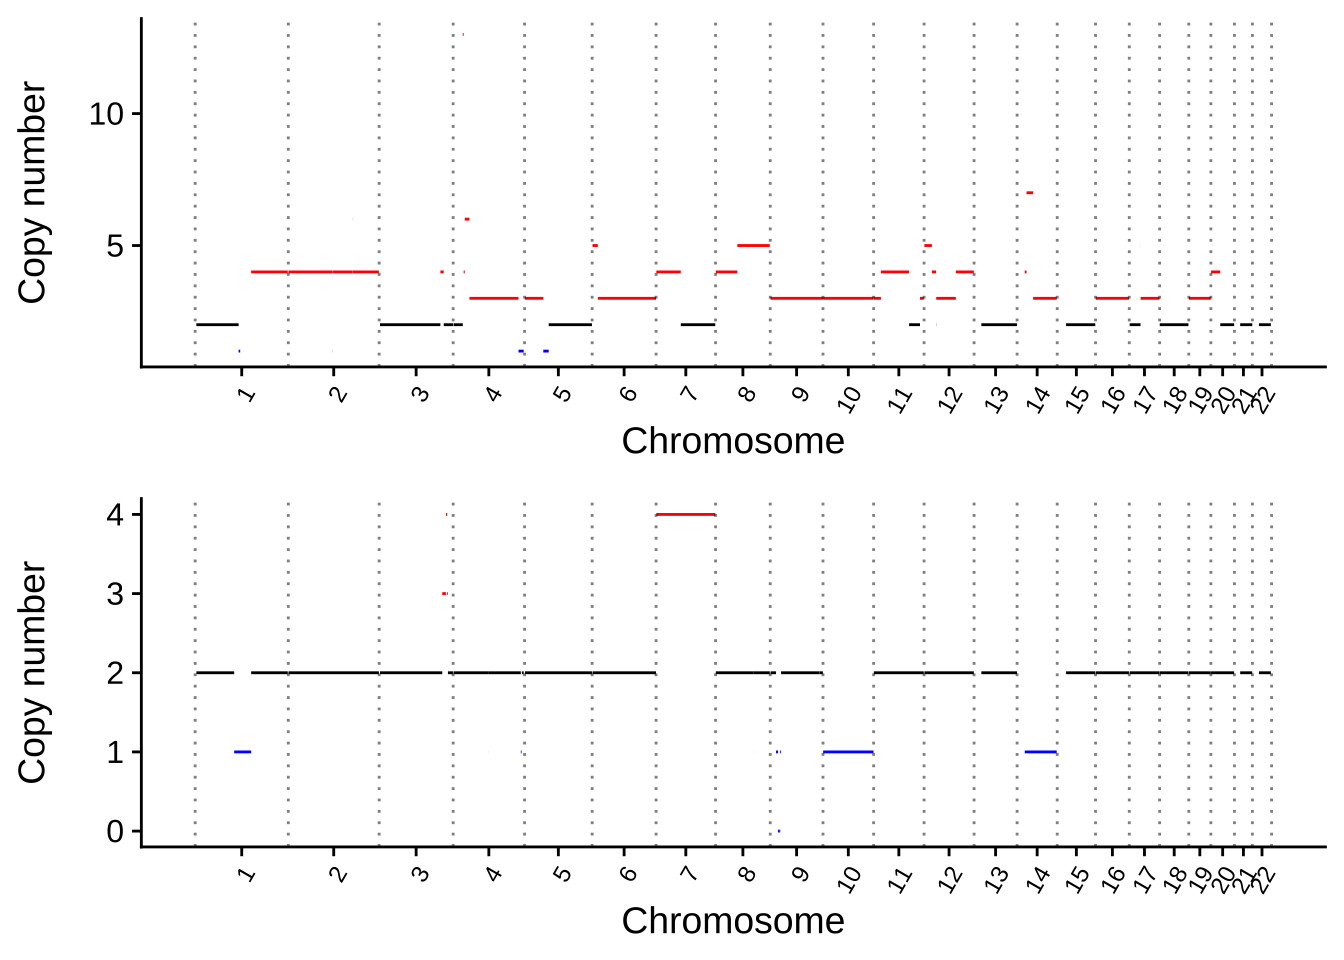
\includegraphics[width=0.95\linewidth]{sigminer_files/figure-latex/unnamed-chunk-68-1}

\begin{Shaded}
\begin{Highlighting}[]
\FunctionTok{show\_cn\_circos}\NormalTok{(cn, }\AttributeTok{samples =} \DecValTok{1}\NormalTok{)}
\end{Highlighting}
\end{Shaded}

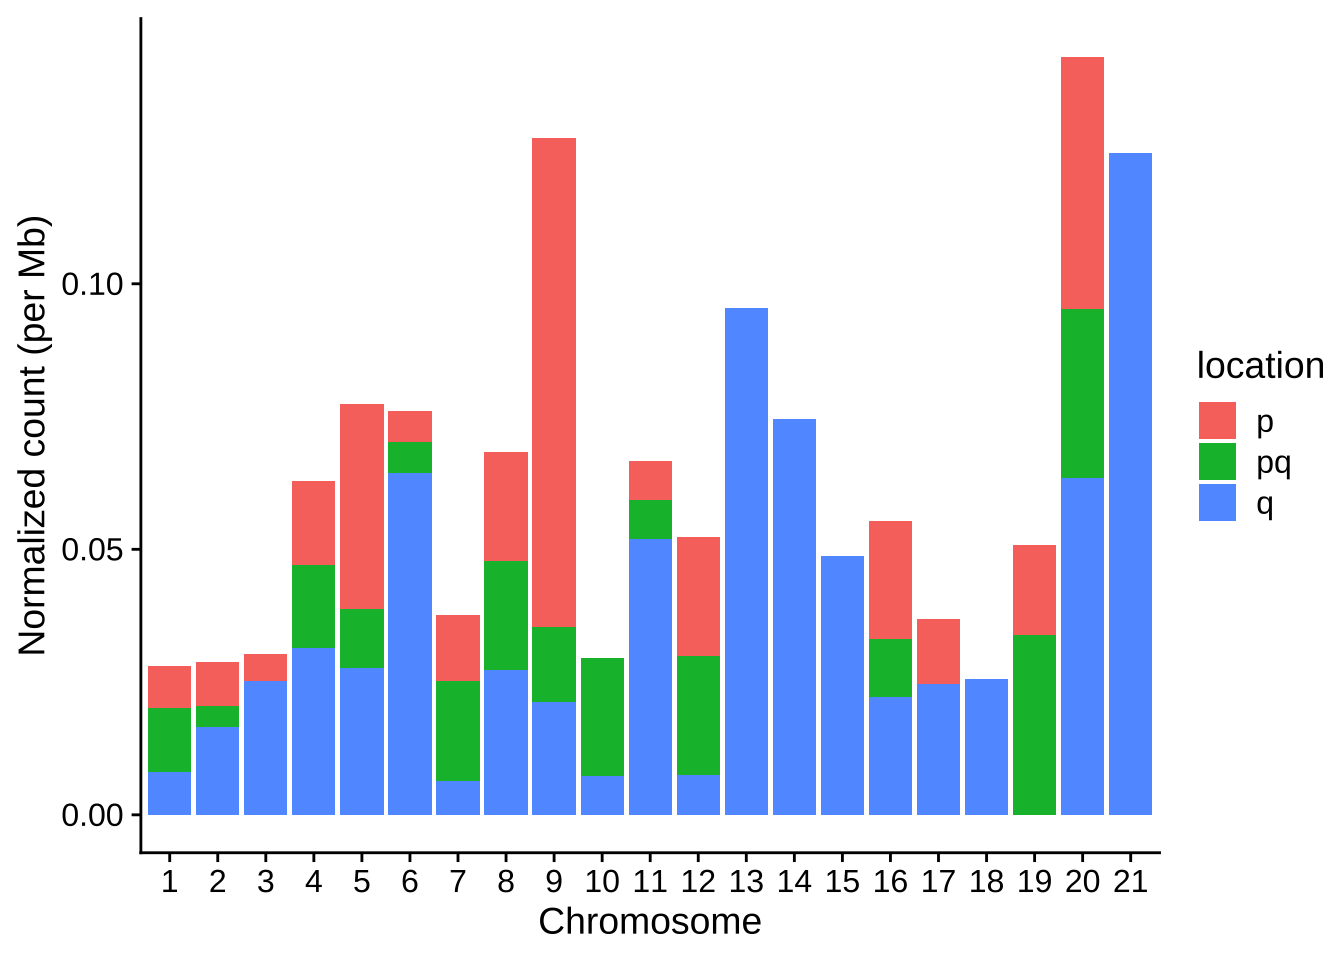
\includegraphics[width=0.95\linewidth]{sigminer_files/figure-latex/unnamed-chunk-69-1}

\hypertarget{distribution}{%
\subsection{Distribution}\label{distribution}}

\begin{Shaded}
\begin{Highlighting}[]
\FunctionTok{show\_cn\_distribution}\NormalTok{(cn, }\AttributeTok{mode =} \StringTok{"ld"}\NormalTok{)}
\end{Highlighting}
\end{Shaded}

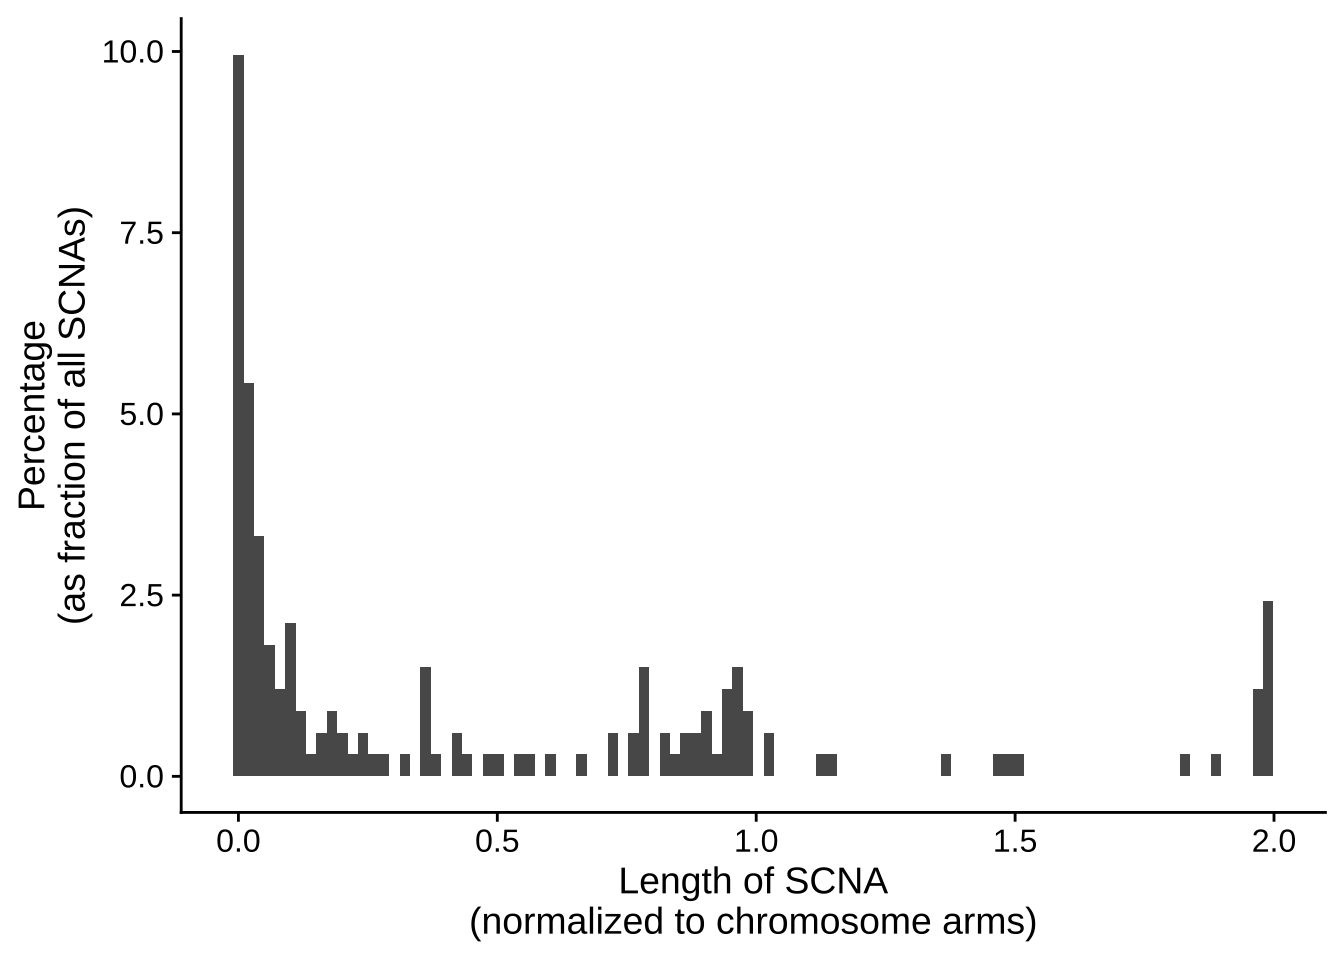
\includegraphics[width=0.95\linewidth]{sigminer_files/figure-latex/unnamed-chunk-70-1}

\begin{Shaded}
\begin{Highlighting}[]
\FunctionTok{show\_cn\_distribution}\NormalTok{(cn, }\AttributeTok{mode =} \StringTok{"cd"}\NormalTok{)}
\end{Highlighting}
\end{Shaded}

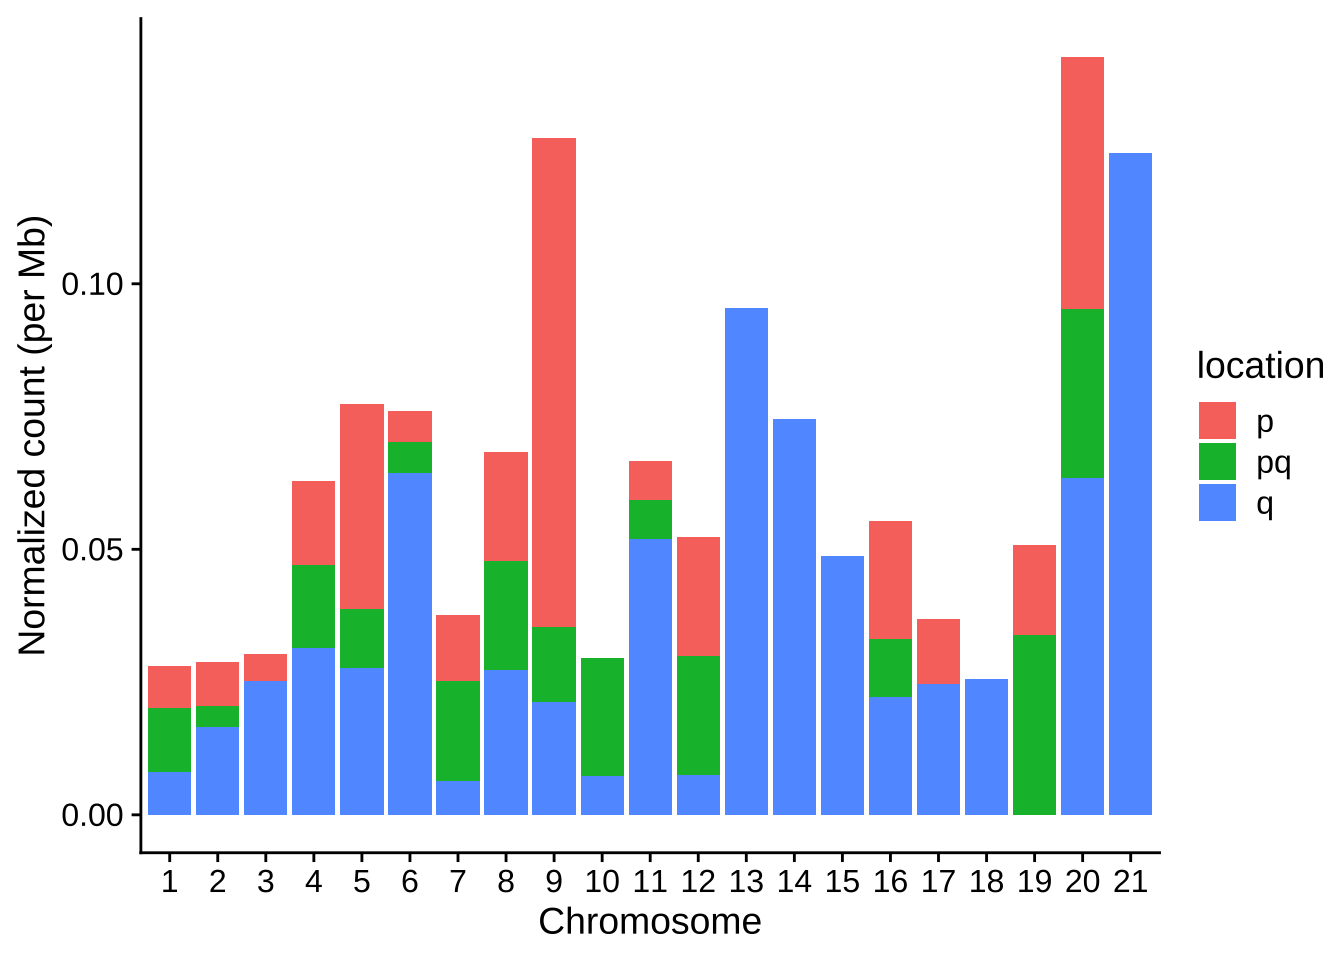
\includegraphics[width=0.95\linewidth]{sigminer_files/figure-latex/unnamed-chunk-71-1}

\hypertarget{signature-object}{%
\section{\texorpdfstring{\texttt{Signature} object}{Signature object}}\label{signature-object}}

\texttt{Signature} is a core object in \textbf{sigminer}, it stores signatures and their exposures. Here we show how to plot signature profile and exposure profile. The result plots are basically \textbf{ggplot} based, so they can be further edited by your custom operations with \textbf{ggplot} grammar.

\hypertarget{operate-signature}{%
\subsection{\texorpdfstring{Operate \texttt{Signature}}{Operate Signature}}\label{operate-signature}}

The result of \texttt{sig\_extract()} or \texttt{sig\_auto\_extract()} is a \texttt{list} with \texttt{Signature} class. You can use \texttt{\$} or use operation function to obtain the data stored in it.

To get the signature matrix:

\begin{Shaded}
\begin{Highlighting}[]
\CommentTok{\# Or mt\_sig2$Signature}
\FunctionTok{sig\_signature}\NormalTok{(mt\_sig2)[}\DecValTok{1}\SpecialCharTok{:}\DecValTok{5}\NormalTok{, ]}
\DocumentationTok{\#\#                Sig1        Sig2         Sig3}
\DocumentationTok{\#\# A[T\textgreater{}C]A 0.008632350 0.012998315 0.0027599263}
\DocumentationTok{\#\# C[T\textgreater{}C]A 0.005765919 0.007065285 0.0007488439}
\DocumentationTok{\#\# G[T\textgreater{}C]A 0.013026940 0.004318256 0.0009744887}
\DocumentationTok{\#\# T[T\textgreater{}C]A 0.004725412 0.004544973 0.0012188315}
\DocumentationTok{\#\# A[C\textgreater{}T]A 0.004464683 0.017714329 0.0063508777}
\end{Highlighting}
\end{Shaded}

To get signature exposure matrix:

\begin{Shaded}
\begin{Highlighting}[]
\CommentTok{\# Or mt\_sig$Exposure}
\FunctionTok{sig\_exposure}\NormalTok{(mt\_sig2)[, }\DecValTok{1}\SpecialCharTok{:}\DecValTok{5}\NormalTok{]}
\DocumentationTok{\#\#      TCGA{-}A1{-}A0SH{-}01A{-}11D{-}A099{-}09 TCGA{-}A2{-}A04N{-}01A{-}11D{-}A10Y{-}09}
\DocumentationTok{\#\# Sig1                     31.66886                    16.840245}
\DocumentationTok{\#\# Sig2                     17.46182                    31.616889}
\DocumentationTok{\#\# Sig3                     86.66939                     3.141982}
\DocumentationTok{\#\#      TCGA{-}A2{-}A0CP{-}01A{-}11W{-}A050{-}09 TCGA{-}A2{-}A0EP{-}01A{-}52D{-}A22X{-}09}
\DocumentationTok{\#\# Sig1                    23.365351                   14.2720018}
\DocumentationTok{\#\# Sig2                    22.090623                    0.7626465}
\DocumentationTok{\#\# Sig3                     4.622696                    6.8293109}
\DocumentationTok{\#\#      TCGA{-}A2{-}A0EV{-}01A{-}11W{-}A050{-}09}
\DocumentationTok{\#\# Sig1                     35.06135}
\DocumentationTok{\#\# Sig2                     25.81997}
\DocumentationTok{\#\# Sig3                     17.46720}
\end{Highlighting}
\end{Shaded}

\texttt{get\_sig\_exposure()} may be more useful, it can be used to return a \texttt{data.frame} and set an exposure threshold.

\begin{Shaded}
\begin{Highlighting}[]
\FunctionTok{get\_sig\_exposure}\NormalTok{(mt\_sig2)}
\DocumentationTok{\#\#                            sample          Sig1          Sig2          Sig3}
\DocumentationTok{\#\#   1: TCGA{-}A1{-}A0SH{-}01A{-}11D{-}A099{-}09  3.166886e+01  1.746182e+01  8.666939e+01}
\DocumentationTok{\#\#   2: TCGA{-}A2{-}A04N{-}01A{-}11D{-}A10Y{-}09  1.684024e+01  3.161689e+01  3.141982e+00}
\DocumentationTok{\#\#   3: TCGA{-}A2{-}A0CP{-}01A{-}11W{-}A050{-}09  2.336535e+01  2.209062e+01  4.622696e+00}
\DocumentationTok{\#\#   4: TCGA{-}A2{-}A0EP{-}01A{-}52D{-}A22X{-}09  1.427200e+01  7.626465e{-}01  6.829311e+00}
\DocumentationTok{\#\#   5: TCGA{-}A2{-}A0EV{-}01A{-}11W{-}A050{-}09  3.506135e+01  2.581997e+01  1.746720e+01}
\DocumentationTok{\#\#   6: TCGA{-}A2{-}A0SX{-}01A{-}12D{-}A099{-}09  1.799211e+01  1.298242e+01  9.594181e+00}
\DocumentationTok{\#\#   7: TCGA{-}A2{-}A0T7{-}01A{-}21D{-}A099{-}09  5.268863e+00  2.400288e+01  4.272836e{-}18}
\DocumentationTok{\#\#   8: TCGA{-}A2{-}A0YF{-}01A{-}21D{-}A10G{-}09  1.304188e+01  2.883374e+01 3.092878e{-}219}
\DocumentationTok{\#\#   9: TCGA{-}A2{-}A25F{-}01A{-}11D{-}A167{-}09  8.954687e+00 2.124482e{-}322  0.000000e+00}
\DocumentationTok{\#\#  10: TCGA{-}A2{-}A3XW{-}01A{-}11D{-}A23C{-}09  9.992137e+00  8.307369e+00  5.585825e{-}01}
\DocumentationTok{\#\#  11: TCGA{-}A2{-}A4S1{-}01A{-}21D{-}A25Q{-}09  6.855788e+01  2.385549e+01  4.218989e+00}
\DocumentationTok{\#\#  12: TCGA{-}A7{-}A0D9{-}01A{-}31W{-}A071{-}09  2.789866e+01  1.612393e+01  1.610362e+01}
\DocumentationTok{\#\#  13: TCGA{-}A7{-}A13F{-}01A{-}11D{-}A12Q{-}09 2.218617e{-}143  7.233318e+01  1.015108e+01}
\DocumentationTok{\#\#  14: TCGA{-}A7{-}A5ZV{-}01A{-}11D{-}A28B{-}09  1.707878e+02  4.282286e+01  3.607406e+01}
\DocumentationTok{\#\#  15: TCGA{-}A8{-}A06P{-}01A{-}11W{-}A019{-}09  2.143307e+01  1.954021e+01  3.290205e+00}
\DocumentationTok{\#\#  16: TCGA{-}A8{-}A076{-}01A{-}21W{-}A019{-}09  3.186376e+01  4.840680e+01  1.219314e+01}
\DocumentationTok{\#\#  17: TCGA{-}A8{-}A07W{-}01A{-}11W{-}A019{-}09  9.941026e+01  4.891769e+01  2.093785e+01}
\DocumentationTok{\#\#  18: TCGA{-}A8{-}A084{-}01A{-}21W{-}A019{-}09  1.860221e+01  3.549728e+01  2.878729e+01}
\DocumentationTok{\#\#  19: TCGA{-}A8{-}A08S{-}01A{-}11W{-}A050{-}09  1.705885e+01  4.703995e+01  2.595490e{-}14}
\DocumentationTok{\#\#  20: TCGA{-}A8{-}A09G{-}01A{-}21W{-}A019{-}09  3.971052e{-}87  1.640886e+01  3.009882e+02}
\DocumentationTok{\#\#  21: TCGA{-}A8{-}A0A4{-}01A{-}11W{-}A019{-}09  1.266228e+01  2.461204e+01  8.855363e{-}01}
\DocumentationTok{\#\#  22: TCGA{-}A8{-}A0AB{-}01A{-}11W{-}A050{-}09  2.161191e+01  1.136710e+01  4.588114e+00}
\DocumentationTok{\#\#  23: TCGA{-}AC{-}A2B8{-}01A{-}11D{-}A17D{-}09 2.033307e{-}122  2.098482e+01  1.038001e+02}
\DocumentationTok{\#\#  24: TCGA{-}AC{-}A2FO{-}01A{-}11D{-}A17W{-}09  8.304307e+00  5.968893e+00  1.455197e+01}
\DocumentationTok{\#\#  25: TCGA{-}AC{-}A3YI{-}01A{-}21D{-}A23C{-}09  1.166597e+01  8.174477e+00 3.737224e{-}304}
\DocumentationTok{\#\#  26: TCGA{-}AC{-}A8OS{-}01A{-}12D{-}A41F{-}09  3.226793e+01  2.847194e+01  1.852043e+01}
\DocumentationTok{\#\#  27: TCGA{-}AN{-}A0FK{-}01A{-}11W{-}A050{-}09 4.675220e{-}136  5.434698e+01 3.013800e{-}322}
\DocumentationTok{\#\#  28: TCGA{-}AN{-}A0FT{-}01A{-}11W{-}A050{-}09  2.329794e+01  6.405417e+01  3.668331e+01}
\DocumentationTok{\#\#  29: TCGA{-}AN{-}A0XO{-}01A{-}11D{-}A10G{-}09  1.810539e+01  1.288004e+01  1.156616e+01}
\DocumentationTok{\#\#  30: TCGA{-}AO{-}A1KS{-}01A{-}11D{-}A13L{-}09  1.471045e{-}15  3.636395e+01  1.884661e+01}
\DocumentationTok{\#\#  31: TCGA{-}AQ{-}A54O{-}01A{-}11D{-}A25Q{-}09 1.998371e{-}110  2.479216e+01  4.475523e{-}01}
\DocumentationTok{\#\#  32: TCGA{-}AQ{-}A7U7{-}01A{-}22D{-}A351{-}09  1.357465e+01  1.450933e+01  7.322714e+01}
\DocumentationTok{\#\#  33: TCGA{-}AR{-}A0TP{-}01A{-}11D{-}A099{-}09  5.700843e+01  7.538727e+00  5.532723e+00}
\DocumentationTok{\#\#  34: TCGA{-}AR{-}A0U3{-}01A{-}11D{-}A10G{-}09  1.566172e+01  2.445972e+01  0.000000e+00}
\DocumentationTok{\#\#  35: TCGA{-}AR{-}A1AH{-}01A{-}11D{-}A12B{-}09  9.313898e+01  1.664222e+01  7.946685e+00}
\DocumentationTok{\#\#  36: TCGA{-}AR{-}A1AJ{-}01A{-}21D{-}A12Q{-}09  7.732463e+00  2.359439e+01  2.272694e+01}
\DocumentationTok{\#\#  37: TCGA{-}AR{-}A1AN{-}01A{-}11D{-}A12Q{-}09  1.050960e{-}43  2.694093e+01  6.145010e+00}
\DocumentationTok{\#\#  38: TCGA{-}AR{-}A24N{-}01A{-}11D{-}A167{-}09  1.894249e+01  2.390942e+01  4.230534e+00}
\DocumentationTok{\#\#  39: TCGA{-}AR{-}A252{-}01A{-}11D{-}A167{-}09  6.071164e+00  1.270826e+01 3.013800e{-}322}
\DocumentationTok{\#\#  40: TCGA{-}AR{-}A2LL{-}01A{-}11D{-}A17W{-}09  1.466495e+01  2.258277e+01 3.013800e{-}322}
\DocumentationTok{\#\#  41: TCGA{-}AR{-}A2LO{-}01A{-}31D{-}A18P{-}09  1.403040e+01  2.614092e+00  3.231288e+00}
\DocumentationTok{\#\#  42: TCGA{-}B6{-}A0IE{-}01A{-}11W{-}A050{-}09  2.010311e+01  1.958096e+01  2.610397e+00}
\DocumentationTok{\#\#  43: TCGA{-}B6{-}A0IM{-}01A{-}11W{-}A050{-}09  2.075968e+01  1.952527e+01 3.513353e{-}125}
\DocumentationTok{\#\#  44: TCGA{-}B6{-}A0IP{-}01A{-}11D{-}A045{-}09  1.416886e+01  3.635690e+01  7.257260e{-}01}
\DocumentationTok{\#\#  45: TCGA{-}B6{-}A0RV{-}01A{-}11D{-}A099{-}09 2.766768e{-}322  1.812611e+01  4.845000e+01}
\DocumentationTok{\#\#  46: TCGA{-}B6{-}A0WZ{-}01A{-}11D{-}A10G{-}09  7.381598e+00  6.159155e+00  8.056780e+01}
\DocumentationTok{\#\#  47: TCGA{-}B6{-}A0X1{-}01A{-}11D{-}A10G{-}09  4.774611e+01  2.081434e+01  2.141664e+01}
\DocumentationTok{\#\#  48: TCGA{-}B6{-}A1KC{-}01B{-}11D{-}A159{-}09  1.224477e+01  2.235468e+01  6.975468e{-}01}
\DocumentationTok{\#\#  49: TCGA{-}B6{-}A401{-}01A{-}11D{-}A23C{-}09  1.104261e+01  1.933849e+01  8.745074e{-}02}
\DocumentationTok{\#\#  50: TCGA{-}B6{-}A40C{-}01A{-}11D{-}A23C{-}09  1.734504e+01  3.269065e+01  2.469909e+00}
\DocumentationTok{\#\#  51: TCGA{-}BH{-}A0AV{-}01A{-}31D{-}A10Y{-}09  6.543456e+01  3.624715e+00  1.540206e+01}
\DocumentationTok{\#\#  52: TCGA{-}BH{-}A0BT{-}01A{-}11D{-}A12Q{-}09  6.306036e+00  3.814813e+01  2.720250e+00}
\DocumentationTok{\#\#  53: TCGA{-}BH{-}A0DL{-}01A{-}11D{-}A10Y{-}09  2.894770e+01  6.846251e+01  2.895576e+01}
\DocumentationTok{\#\#  54: TCGA{-}BH{-}A0DO{-}01B{-}11D{-}A12B{-}09  9.969784e+00  1.446941e+01  5.233825e+00}
\DocumentationTok{\#\#  55: TCGA{-}BH{-}A0DT{-}01A{-}21D{-}A12B{-}09  2.462409e+00  1.154792e+01  1.819875e+00}
\DocumentationTok{\#\#  56: TCGA{-}BH{-}A0GY{-}01A{-}11W{-}A071{-}09  1.621720e+01  2.581025e+01 4.526295e{-}276}
\DocumentationTok{\#\#  57: TCGA{-}BH{-}A0H6{-}01A{-}21W{-}A071{-}09  1.082937e+01  1.579577e+01 4.340126e{-}293}
\DocumentationTok{\#\#  58: TCGA{-}BH{-}A18K{-}01A{-}11D{-}A12B{-}09  2.097981e+01  1.462527e+01  3.631013e+01}
\DocumentationTok{\#\#  59: TCGA{-}BH{-}A1FU{-}01A{-}11D{-}A14G{-}09  6.277453e+01  2.878294e+01  2.394254e+01}
\DocumentationTok{\#\#  60: TCGA{-}BH{-}A202{-}01A{-}11D{-}A14K{-}09  6.871836e+00  2.020375e+01  3.928063e{-}01}
\DocumentationTok{\#\#  61: TCGA{-}BH{-}A5IZ{-}01A{-}11D{-}A27P{-}09  1.246154e+02  2.209061e+01  3.537264e+01}
\DocumentationTok{\#\#  62: TCGA{-}BH{-}A6R8{-}01A{-}21D{-}A33E{-}09  1.164019e+01  2.430453e+01  5.236235e+00}
\DocumentationTok{\#\#  63: TCGA{-}BH{-}A8G0{-}01A{-}11D{-}A351{-}09 2.597199e{-}102  2.048118e+01  0.000000e+00}
\DocumentationTok{\#\#  64: TCGA{-}C8{-}A131{-}01A{-}11D{-}A10Y{-}09  2.590583e+01  4.370584e+01  3.640790e+00}
\DocumentationTok{\#\#  65: TCGA{-}D8{-}A147{-}01A{-}11D{-}A10Y{-}09  1.161776e+02  5.212590e+00  7.266037e+01}
\DocumentationTok{\#\#  66: TCGA{-}D8{-}A1JG{-}01B{-}11D{-}A13L{-}09  8.471905e+01  6.345205e+01  2.060929e+01}
\DocumentationTok{\#\#  67: TCGA{-}D8{-}A1JH{-}01A{-}11D{-}A188{-}09  9.663174e+00  1.327837e+01  7.873566e{-}01}
\DocumentationTok{\#\#  68: TCGA{-}D8{-}A1JJ{-}01A{-}31D{-}A14K{-}09  1.133959e+01  3.674766e+01  5.104066e+01}
\DocumentationTok{\#\#  69: TCGA{-}D8{-}A1JT{-}01A{-}31D{-}A13L{-}09  2.090274e+01  2.128976e+01  0.000000e+00}
\DocumentationTok{\#\#  70: TCGA{-}D8{-}A1JU{-}01A{-}11D{-}A13L{-}09  9.091898e+00  1.071928e+01  2.713162e{-}39}
\DocumentationTok{\#\#  71: TCGA{-}D8{-}A1X7{-}01A{-}11D{-}A14K{-}09  1.294633e+01  1.525286e+01  3.413301e+00}
\DocumentationTok{\#\#  72: TCGA{-}D8{-}A1X8{-}01A{-}11D{-}A14K{-}09  1.448665e+01  1.581697e+01  2.266142e+00}
\DocumentationTok{\#\#  73: TCGA{-}D8{-}A1XL{-}01A{-}11D{-}A14K{-}09  7.589129e+01  2.279192e+01  7.395903e+00}
\DocumentationTok{\#\#  74: TCGA{-}D8{-}A27V{-}01A{-}12D{-}A17D{-}09  3.423782e{-}80  3.137792e+01  1.880720e+02}
\DocumentationTok{\#\#  75: TCGA{-}E2{-}A108{-}01A{-}13D{-}A10M{-}09  3.632974e+01  1.314449e+01  1.338054e+02}
\DocumentationTok{\#\#  76: TCGA{-}E2{-}A10F{-}01A{-}11D{-}A10M{-}09 2.766768e{-}322  2.414387e+01  5.123782e+00}
\DocumentationTok{\#\#  77: TCGA{-}E2{-}A14T{-}01A{-}11D{-}A10Y{-}09  1.661234e+01  1.927166e+01  7.476472e+00}
\DocumentationTok{\#\#  78: TCGA{-}E2{-}A152{-}01A{-}11D{-}A12B{-}09  1.171920e{-}21  1.987249e+01  1.445783e+02}
\DocumentationTok{\#\#  79: TCGA{-}E2{-}A15D{-}01A{-}11D{-}A10Y{-}09  1.162797e+01  2.447046e+01  8.456098e{-}02}
\DocumentationTok{\#\#  80: TCGA{-}E2{-}A15L{-}01A{-}11D{-}A12B{-}09 6.564409e{-}266  3.705154e+01  7.227903e+00}
\DocumentationTok{\#\#  81: TCGA{-}E2{-}A1BD{-}01A{-}11D{-}A12Q{-}09  1.347320e+01  2.835382e+01  7.608654e{-}02}
\DocumentationTok{\#\#  82: TCGA{-}E2{-}A1IH{-}01A{-}11D{-}A188{-}09  1.607014e+01  2.769621e+01  4.043042e+01}
\DocumentationTok{\#\#  83: TCGA{-}E2{-}A1II{-}01A{-}11D{-}A142{-}09  3.287852e+01  1.507799e+00 3.013800e{-}322}
\DocumentationTok{\#\#  84: TCGA{-}E2{-}A1IJ{-}01A{-}11D{-}A142{-}09  6.353640e+00  1.340142e+01 1.066686e{-}292}
\DocumentationTok{\#\#  85: TCGA{-}E2{-}A1L6{-}01A{-}11D{-}A13L{-}09  2.115141e{-}46  2.802838e+01  7.333578e{-}63}
\DocumentationTok{\#\#  86: TCGA{-}E2{-}A9RU{-}01A{-}11D{-}A41F{-}09  2.027101e+01  6.333655e+01  2.100747e+01}
\DocumentationTok{\#\#  87: TCGA{-}E9{-}A1NE{-}01A{-}21D{-}A14K{-}09  4.944191e+01  5.057375e+00  6.071713e+00}
\DocumentationTok{\#\#  88: TCGA{-}E9{-}A22A{-}01A{-}11D{-}A159{-}09  1.889911e+01  7.690585e+00  1.009118e+01}
\DocumentationTok{\#\#  89: TCGA{-}E9{-}A22E{-}01A{-}11D{-}A159{-}09  9.223014e+01  1.041757e+01  4.455073e+01}
\DocumentationTok{\#\#  90: TCGA{-}E9{-}A3QA{-}01A{-}61D{-}A228{-}09  3.257514e+01  4.527811e+00  2.793381e+01}
\DocumentationTok{\#\#  91: TCGA{-}E9{-}A5FL{-}01A{-}11D{-}A27P{-}09  9.051438e+01  1.322275e+01  2.905100e+01}
\DocumentationTok{\#\#  92: TCGA{-}EW{-}A1PA{-}01A{-}11D{-}A142{-}09  1.887140e+01  1.923060e+01  4.231605e+00}
\DocumentationTok{\#\#  93: TCGA{-}EW{-}A1PH{-}01A{-}11D{-}A14K{-}09  2.347811e+01  3.271478e+01  8.143171e+00}
\DocumentationTok{\#\#  94: TCGA{-}GM{-}A2DB{-}01A{-}31D{-}A19Y{-}09  8.399491e+01  3.122550e+01  1.350770e+01}
\DocumentationTok{\#\#  95: TCGA{-}LD{-}A9QF{-}01A{-}32D{-}A41F{-}09  1.456385e+01  2.328753e+01  1.357230e+00}
\DocumentationTok{\#\#  96: TCGA{-}LL{-}A5YP{-}01A{-}21D{-}A28B{-}09  7.878814e+01  6.897847e+00  2.056396e+01}
\DocumentationTok{\#\#  97: TCGA{-}LL{-}A73Z{-}01A{-}11D{-}A32I{-}09  2.436630e+01  2.686392e+01  2.538904e+00}
\DocumentationTok{\#\#  98: TCGA{-}OL{-}A5RY{-}01A{-}21D{-}A28B{-}09  7.360216e+00  7.184128e+00  1.360407e+00}
\DocumentationTok{\#\#  99: TCGA{-}PE{-}A5DD{-}01A{-}12D{-}A27P{-}09  3.562644e+00  3.773066e+01  4.313237e+01}
\DocumentationTok{\#\# 100: TCGA{-}S3{-}AA17{-}01A{-}11D{-}A41F{-}09  9.349168e+01  2.892403e+01  2.042929e+01}
\DocumentationTok{\#\#                            sample          Sig1          Sig2          Sig3}
\end{Highlighting}
\end{Shaded}

\hypertarget{signature-profile}{%
\subsection{Signature profile}\label{signature-profile}}

A signature is composed of distinct component patterns. They can be shown by \texttt{show\_sig\_profile()}. Of note, for different types of signature, the bar heights may have different meanings.

\begin{itemize}
\tightlist
\item
  SBS signatures are displayed based on the observed component frequency of the human genome, i.e., representing the relative proportions of mutations generated by each signature based on the actual trinucleotide frequencies of the reference human genome.
\item
  Similar to SBS signatures, copy number signatures are displayed based on the observed component frequency of the human genome. Of note, considering the count process of each feature is relatively independent, the profile is row normalized by each feature, unlike Macintyre et al.~(2018) did column normalization (this method is easy to mislead readers), so the bar height can be compared within/between features.
\end{itemize}

\hypertarget{sbs-signature-profile}{%
\subsection{SBS signature profile}\label{sbs-signature-profile}}

\begin{Shaded}
\begin{Highlighting}[]
\FunctionTok{show\_sig\_profile}\NormalTok{(mt\_sig, }\AttributeTok{mode =} \StringTok{"SBS"}\NormalTok{, }\AttributeTok{paint\_axis\_text =} \ConstantTok{FALSE}\NormalTok{, }\AttributeTok{x\_label\_angle =} \DecValTok{90}\NormalTok{)}
\end{Highlighting}
\end{Shaded}

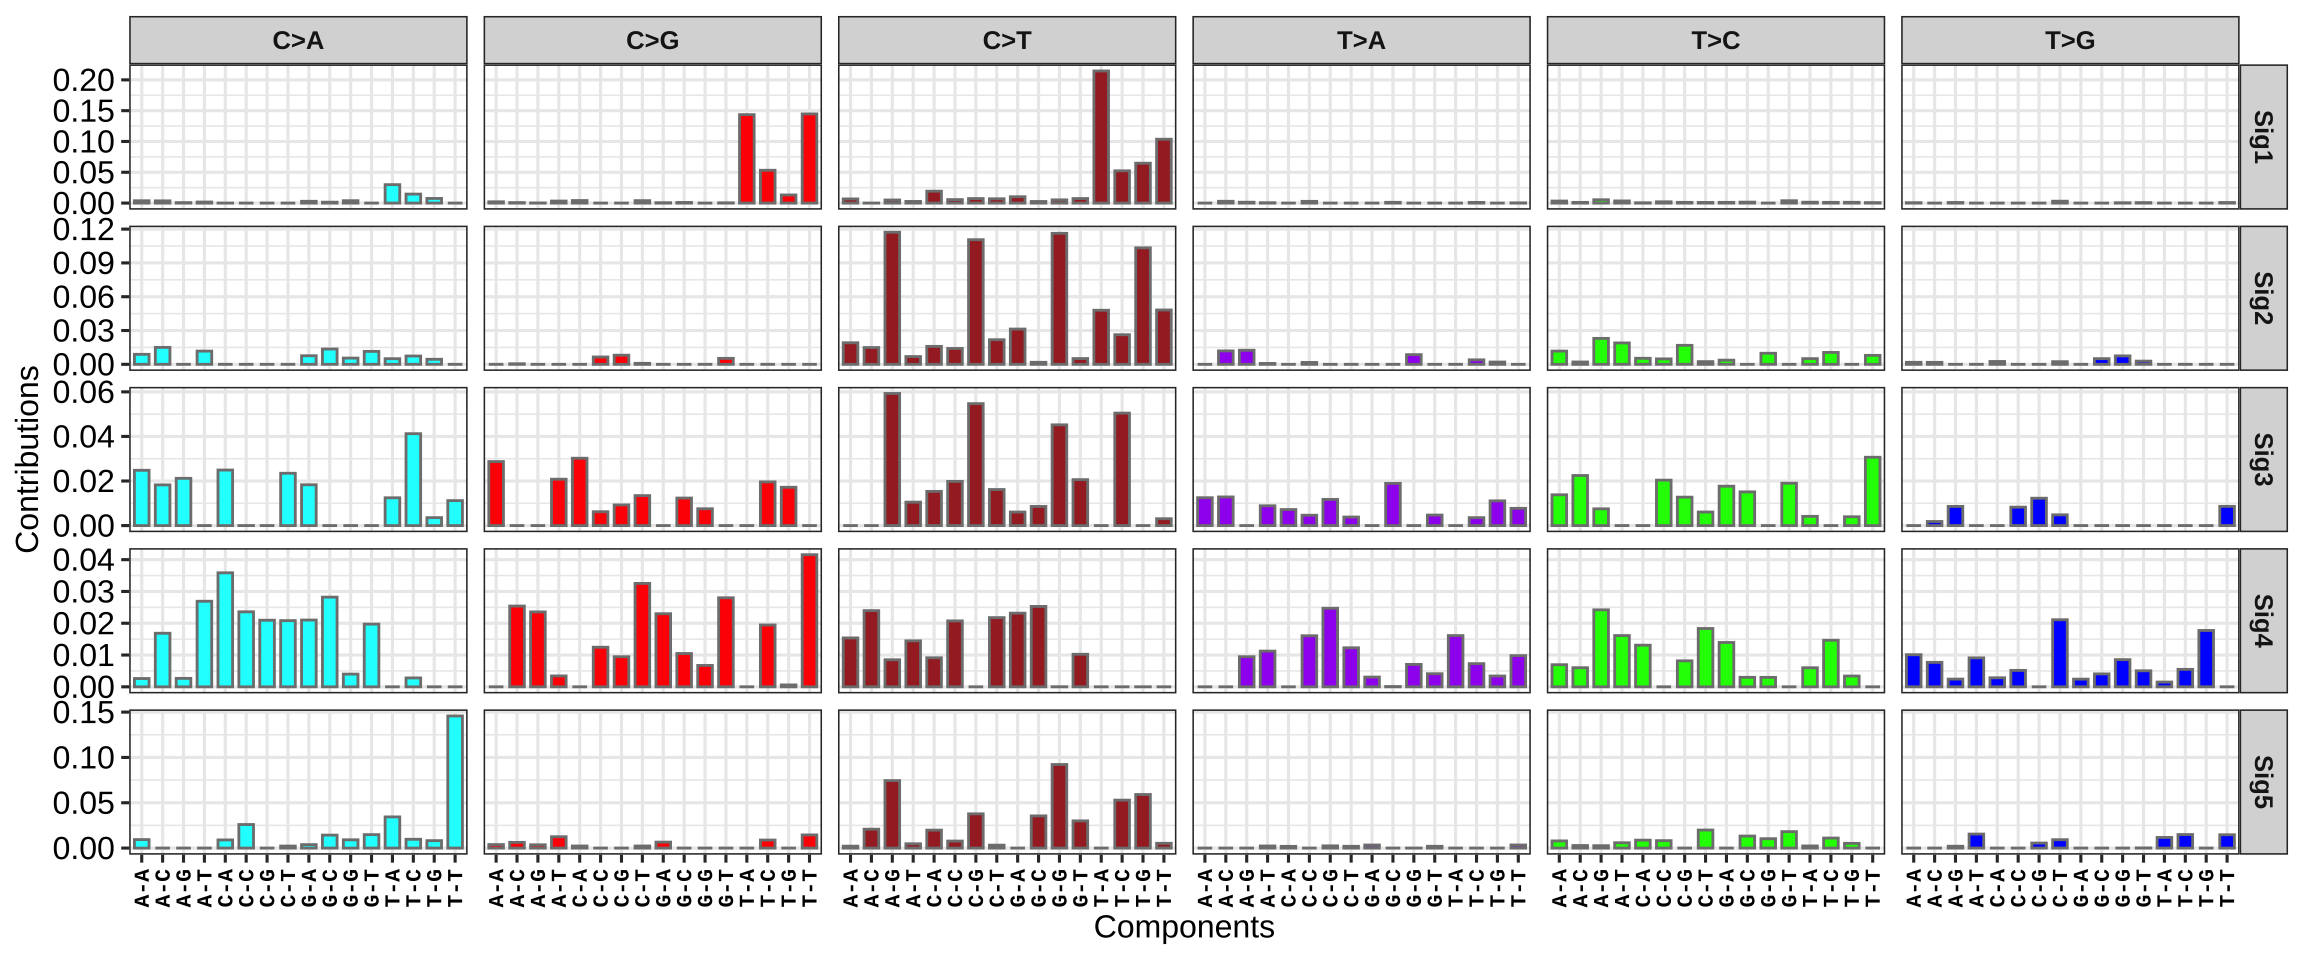
\includegraphics[width=0.95\linewidth]{sigminer_files/figure-latex/unnamed-chunk-75-1}

\begin{Shaded}
\begin{Highlighting}[]
\FunctionTok{show\_sig\_profile}\NormalTok{(mt\_sig, }\AttributeTok{mode =} \StringTok{"SBS"}\NormalTok{, }\AttributeTok{style =} \StringTok{"cosmic"}\NormalTok{, }\AttributeTok{x\_label\_angle =} \DecValTok{90}\NormalTok{)}
\end{Highlighting}
\end{Shaded}

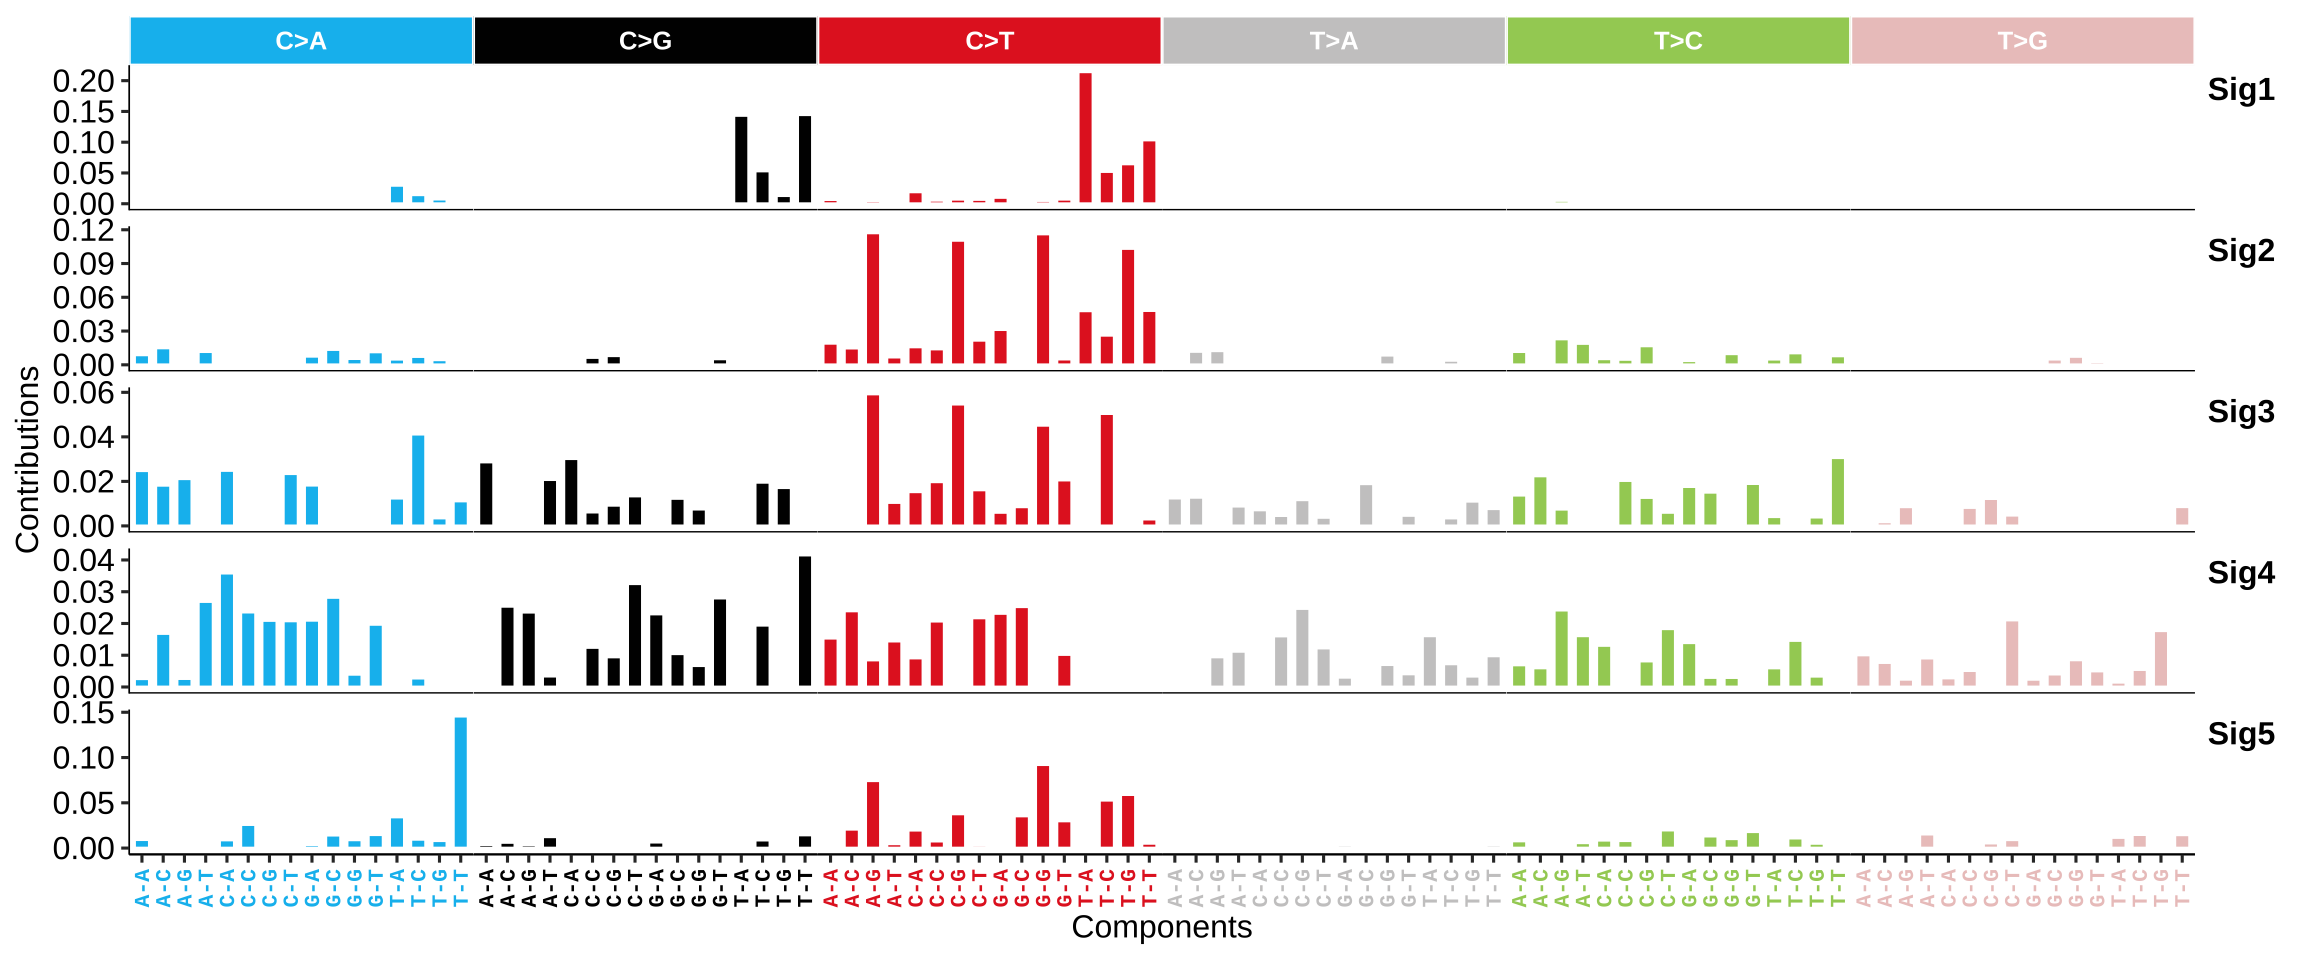
\includegraphics[width=0.95\linewidth]{sigminer_files/figure-latex/unnamed-chunk-76-1}

\hypertarget{copy-number-signature-profile}{%
\subsection{Copy number signature profile}\label{copy-number-signature-profile}}

For copy number signatures from tally method ``W'', you have to specify the \texttt{normalize} option as ``feature'', so the bar heights can be more clearly compared.

\begin{Shaded}
\begin{Highlighting}[]
\FunctionTok{show\_sig\_profile}\NormalTok{(sig\_w,}
  \AttributeTok{mode =} \StringTok{"copynumber"}\NormalTok{,}
  \AttributeTok{normalize =} \StringTok{"feature"}\NormalTok{,}
  \AttributeTok{method =} \StringTok{"W"}\NormalTok{,}
  \AttributeTok{style =} \StringTok{"cosmic"}
\NormalTok{)}
\end{Highlighting}
\end{Shaded}

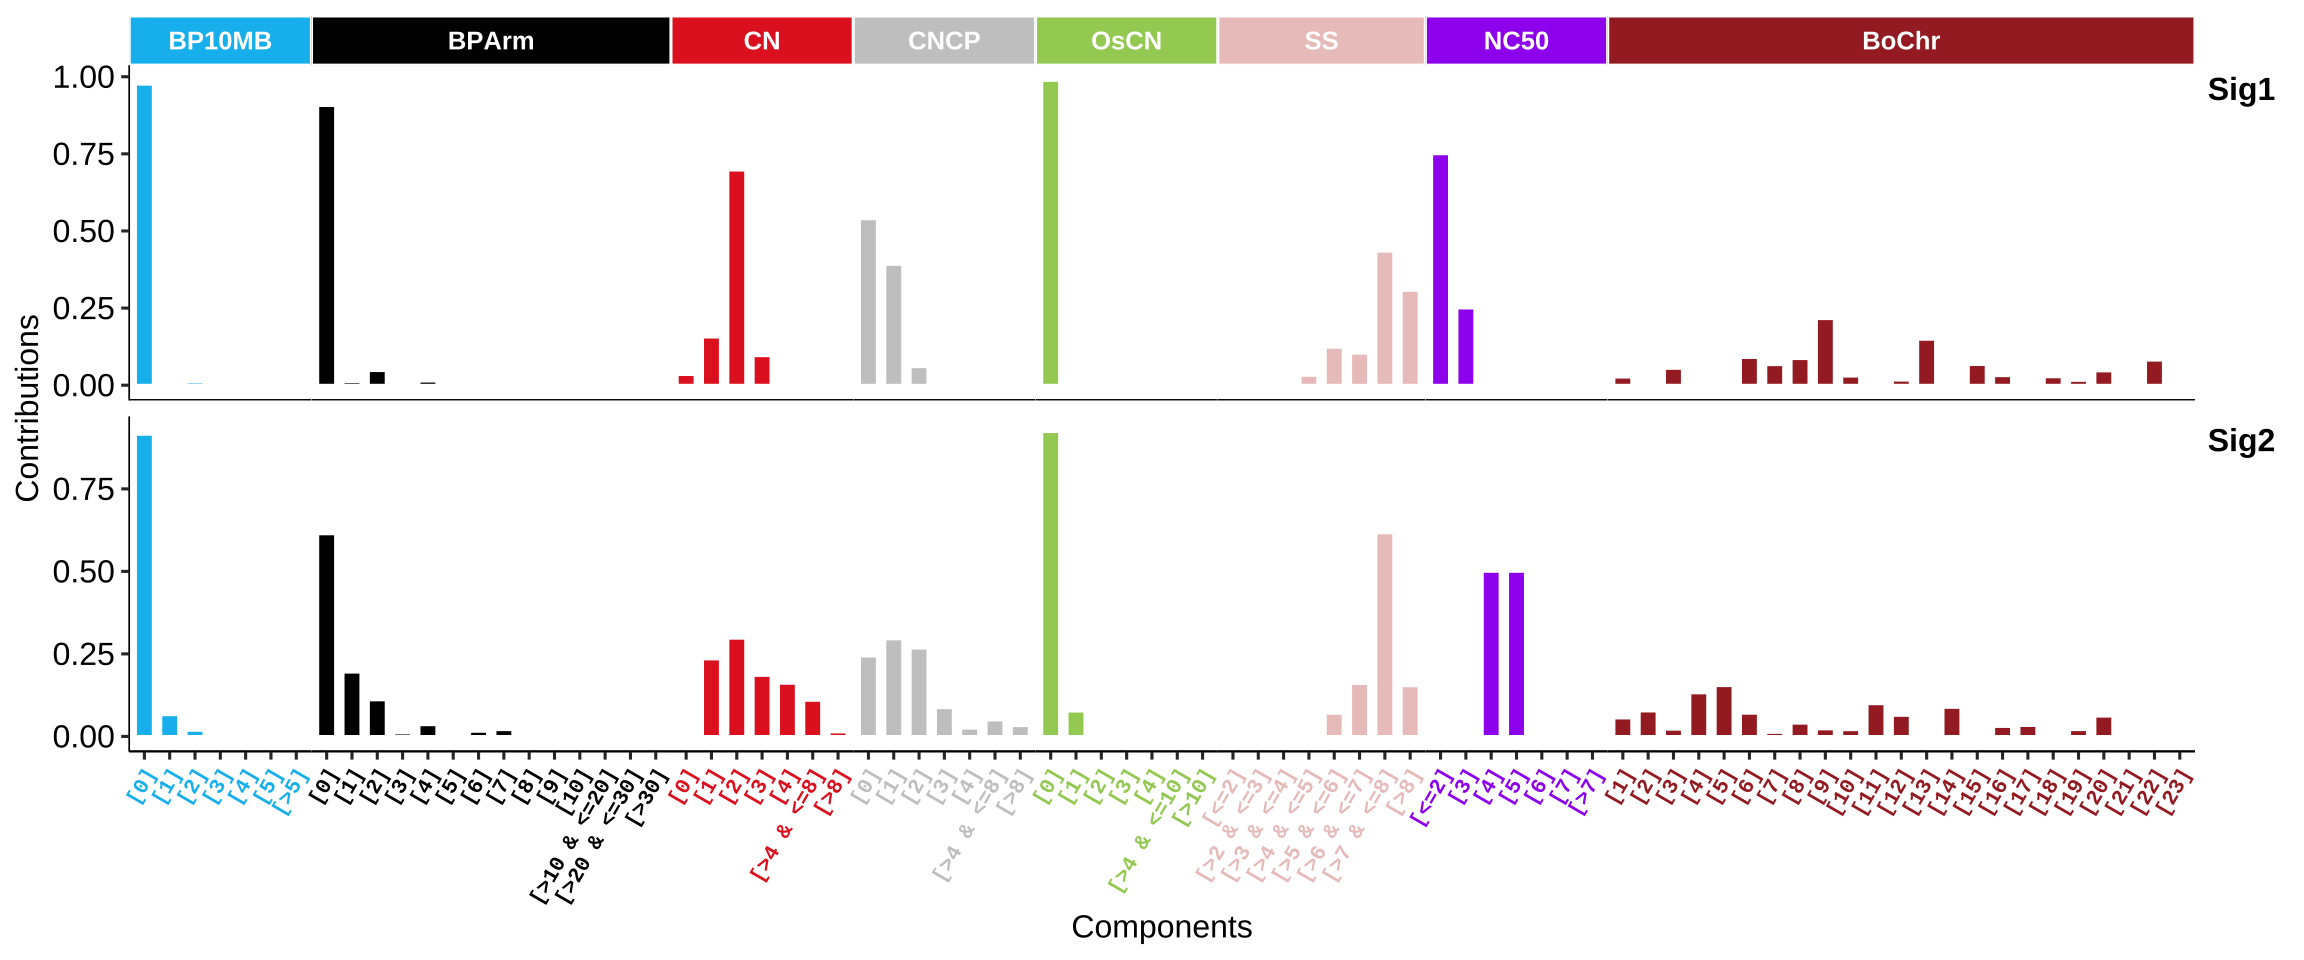
\includegraphics[width=0.95\linewidth]{sigminer_files/figure-latex/unnamed-chunk-77-1}

\hypertarget{cosmic-signature-profile}{%
\subsection{COSMIC signature profile}\label{cosmic-signature-profile}}

Users can show profile of COSMIC signatures by \texttt{show\_cosmic\_sig\_profile()}.

To see valid signature numbers, run

\begin{Shaded}
\begin{Highlighting}[]
\FunctionTok{show\_cosmic\_sig\_profile}\NormalTok{(}\AttributeTok{sig\_db =} \StringTok{"legacy"}\NormalTok{)}
\DocumentationTok{\#\# }
\DocumentationTok{\#\# Valid index for db \textquotesingle{}legacy\textquotesingle{}:}
\DocumentationTok{\#\# 1 2 3 4 5 6 7 8 9 10 11 12 13 14 15 16 17 18 19 20 21 22 23 24 25 26 27 28 29 30}
\end{Highlighting}
\end{Shaded}

\begin{quote}
`legacy' is for COSMIC v2.
\end{quote}

\begin{Shaded}
\begin{Highlighting}[]
\FunctionTok{show\_cosmic\_sig\_profile}\NormalTok{(}\AttributeTok{sig\_db =} \StringTok{"SBS"}\NormalTok{)}
\DocumentationTok{\#\# }
\DocumentationTok{\#\# Valid index for db \textquotesingle{}SBS\textquotesingle{}:}
\DocumentationTok{\#\# 1 2 3 4 5 6 7a 7b 7c 7d 8 9 10a 10b 11 12 13 14 15 16 17a 17b 18 19 20 21 22 23 24 25 26 27 28 29 30 31 32 33 34 35 36 37 38 39 40 41 42 43 44 45 46 47 48 49 50 51 52 53 54 55 56 57 58 59 60 84 85 86 87 88 89 90}
\end{Highlighting}
\end{Shaded}

To show the plot, specify signature shortnames to \texttt{sig\_index} option.

\begin{Shaded}
\begin{Highlighting}[]
\FunctionTok{show\_cosmic\_sig\_profile}\NormalTok{(}\AttributeTok{sig\_index =} \FunctionTok{c}\NormalTok{(}\DecValTok{1}\NormalTok{, }\DecValTok{5}\NormalTok{, }\DecValTok{6}\NormalTok{), }\AttributeTok{style =} \StringTok{"cosmic"}\NormalTok{)}
\DocumentationTok{\#\# }
\DocumentationTok{\#\# Valid index for db \textquotesingle{}legacy\textquotesingle{}:}
\DocumentationTok{\#\# 1 2 3 4 5 6 7 8 9 10 11 12 13 14 15 16 17 18 19 20 21 22 23 24 25 26 27 28 29 30}
\end{Highlighting}
\end{Shaded}

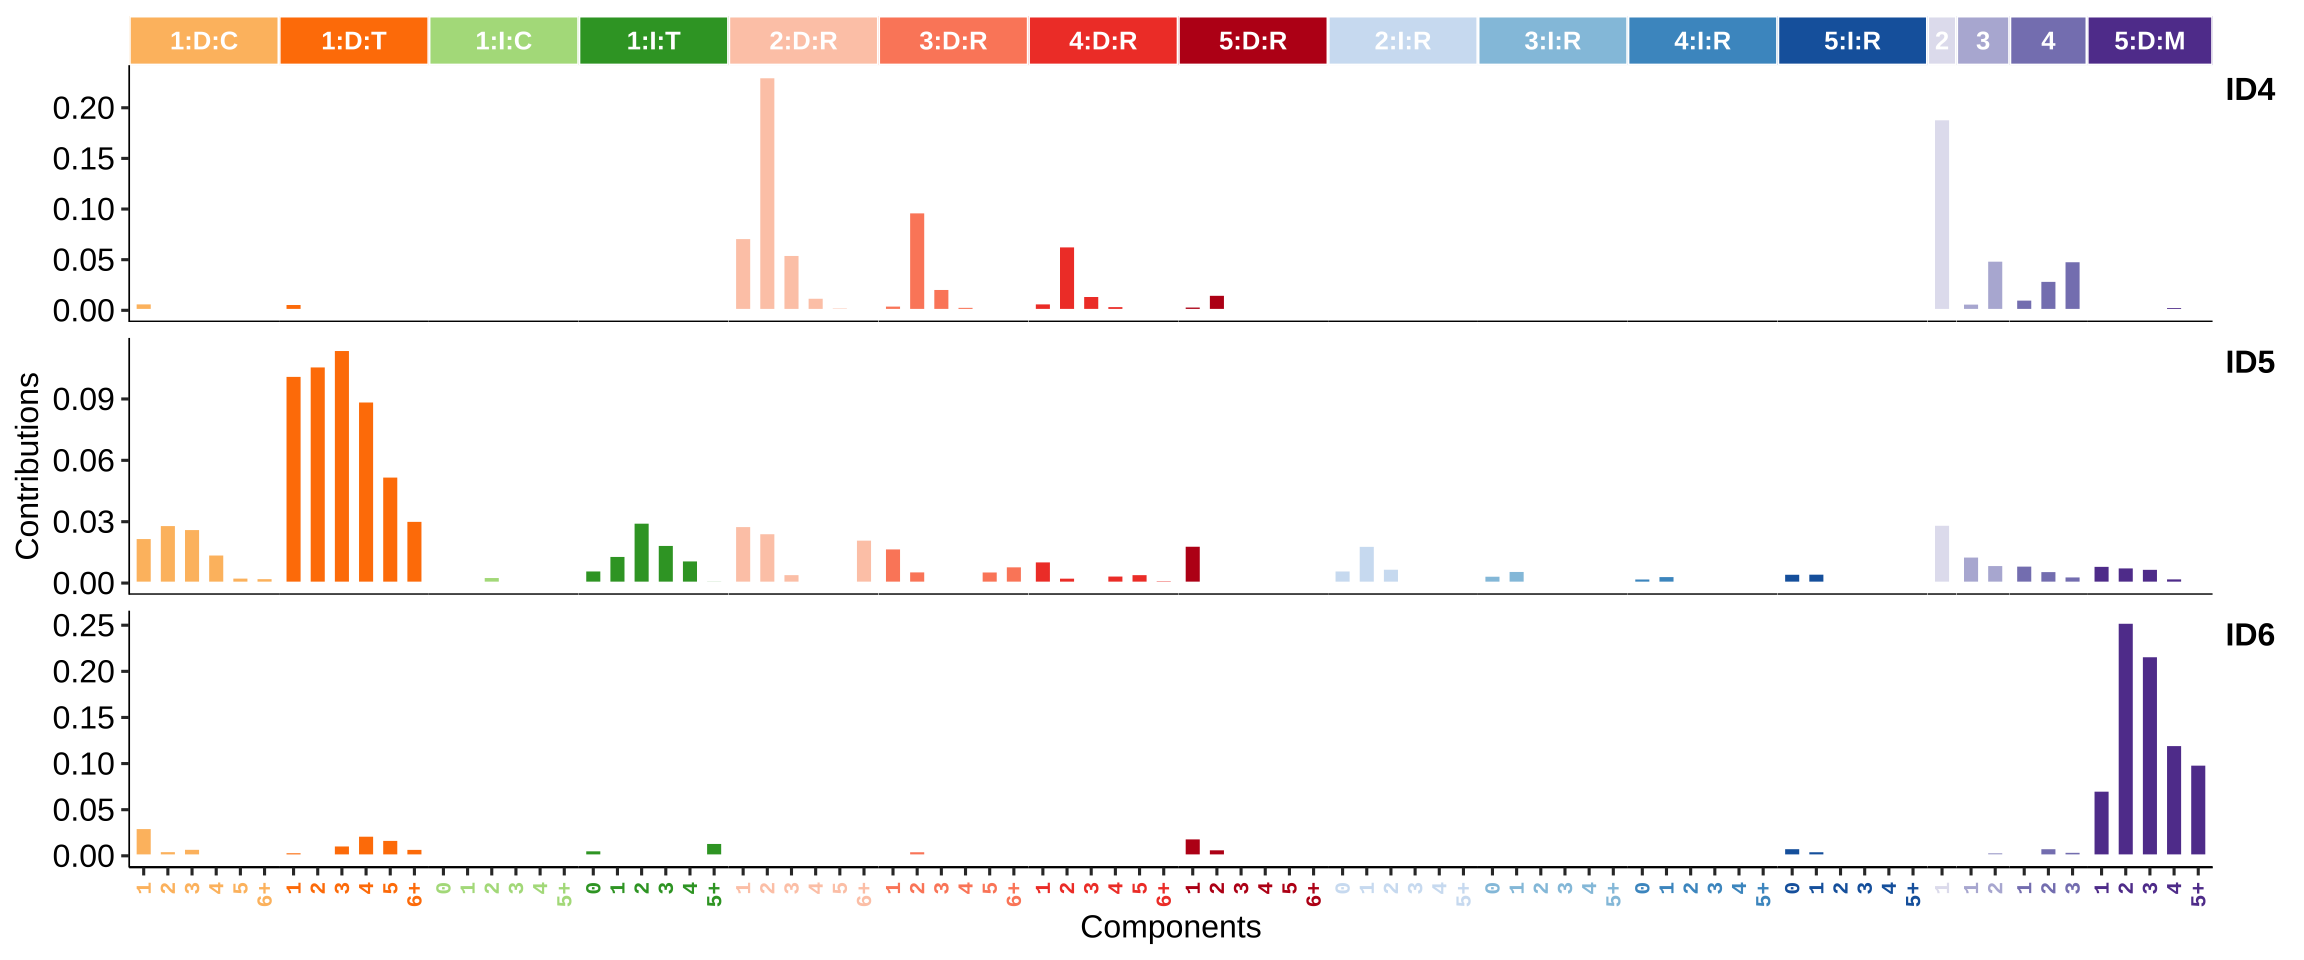
\includegraphics[width=0.95\linewidth]{sigminer_files/figure-latex/unnamed-chunk-80-1}

\begin{Shaded}
\begin{Highlighting}[]
\FunctionTok{show\_cosmic\_sig\_profile}\NormalTok{(}\AttributeTok{sig\_index =} \FunctionTok{c}\NormalTok{(}\DecValTok{1}\NormalTok{, }\DecValTok{2}\NormalTok{, }\DecValTok{3}\NormalTok{), }\AttributeTok{style =} \StringTok{"cosmic"}\NormalTok{, }\AttributeTok{sig\_db =} \StringTok{"DBS"}\NormalTok{)}
\DocumentationTok{\#\# }
\DocumentationTok{\#\# Valid index for db \textquotesingle{}DBS\textquotesingle{}:}
\DocumentationTok{\#\# 1 2 3 4 5 6 7 8 9 10 11}
\end{Highlighting}
\end{Shaded}

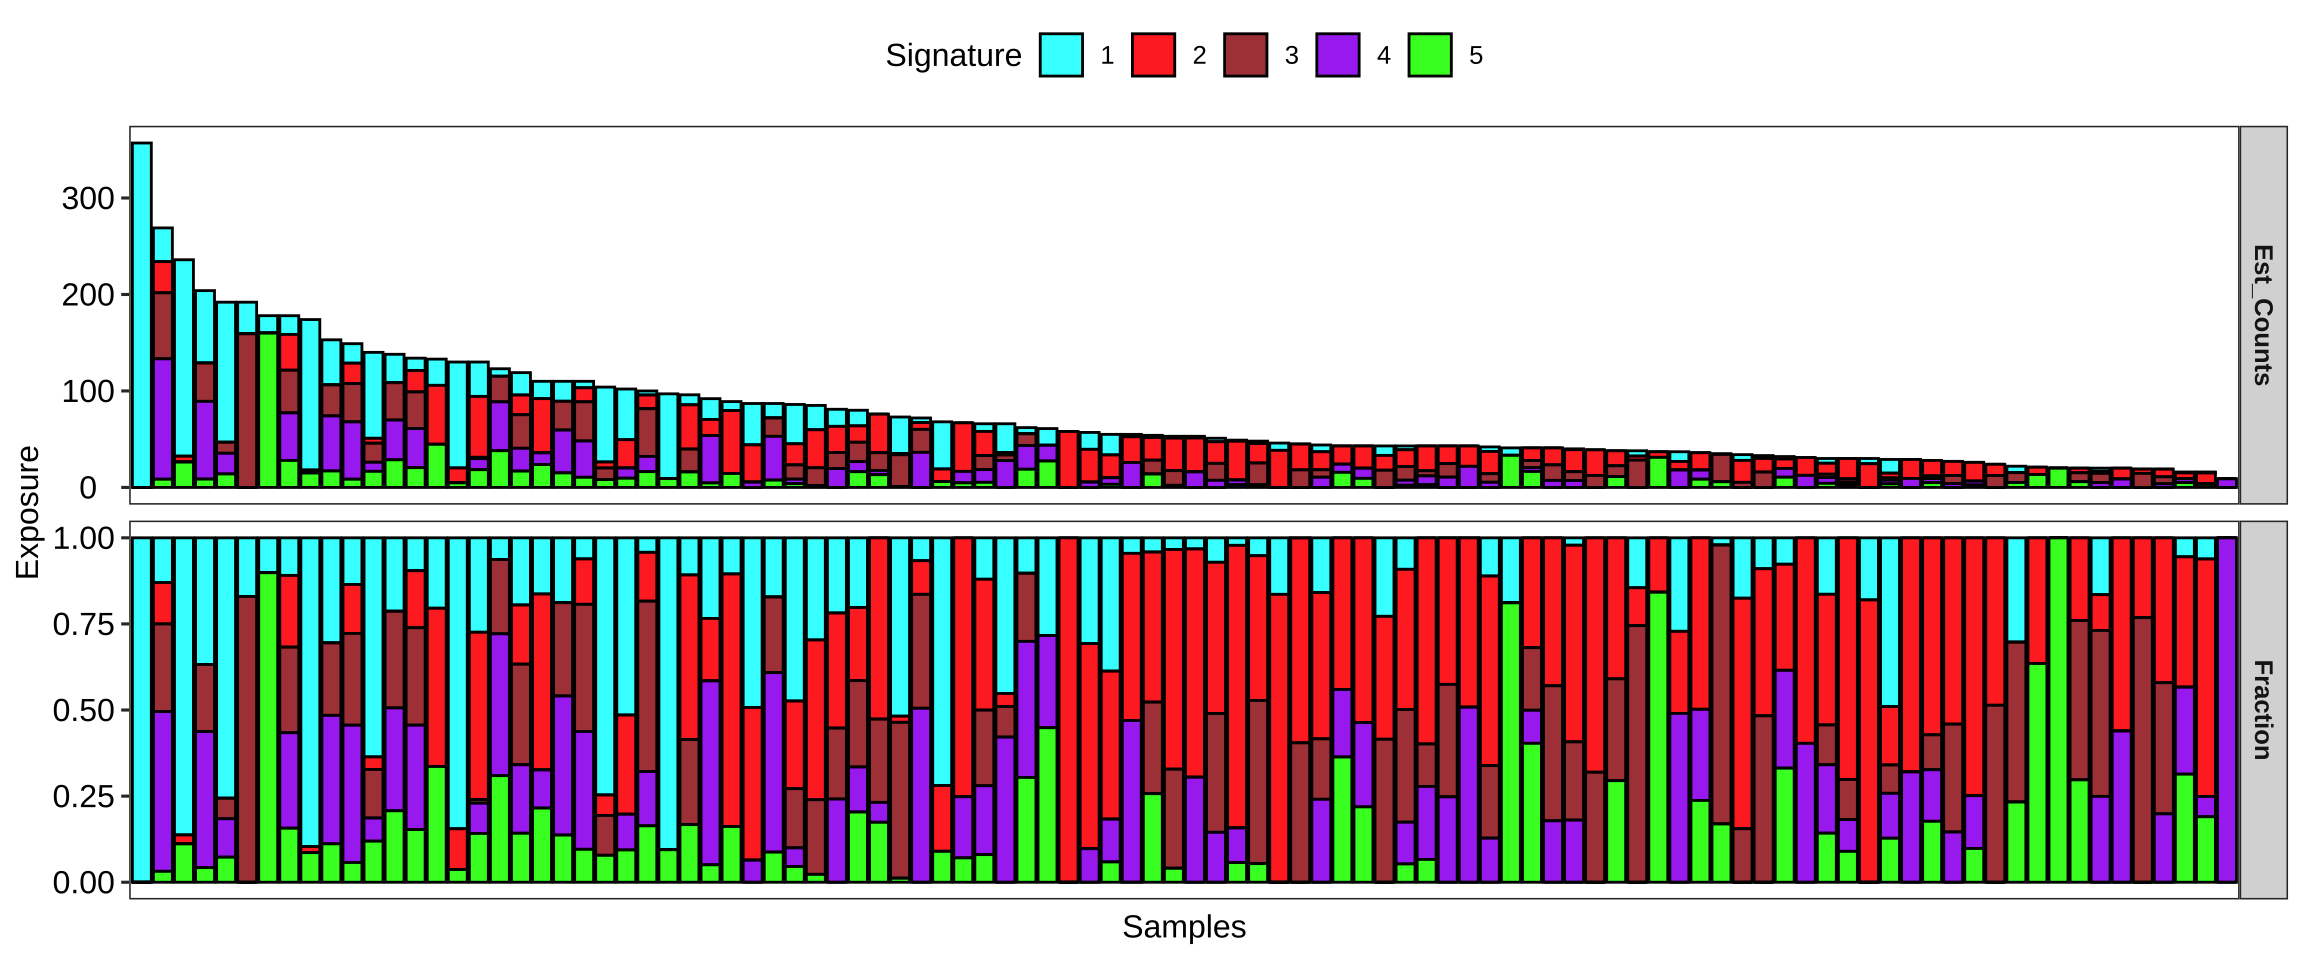
\includegraphics[width=0.95\linewidth]{sigminer_files/figure-latex/unnamed-chunk-81-1}

\begin{Shaded}
\begin{Highlighting}[]
\FunctionTok{show\_cosmic\_sig\_profile}\NormalTok{(}\AttributeTok{sig\_index =} \FunctionTok{c}\NormalTok{(}\DecValTok{4}\NormalTok{, }\DecValTok{5}\NormalTok{, }\DecValTok{6}\NormalTok{), }\AttributeTok{style =} \StringTok{"cosmic"}\NormalTok{, }\AttributeTok{sig\_db =} \StringTok{"ID"}\NormalTok{)}
\DocumentationTok{\#\# }
\DocumentationTok{\#\# Valid index for db \textquotesingle{}ID\textquotesingle{}:}
\DocumentationTok{\#\# 1 2 3 4 5 6 7 8 9 10 11 12 13 14 15 16 17 18}
\end{Highlighting}
\end{Shaded}

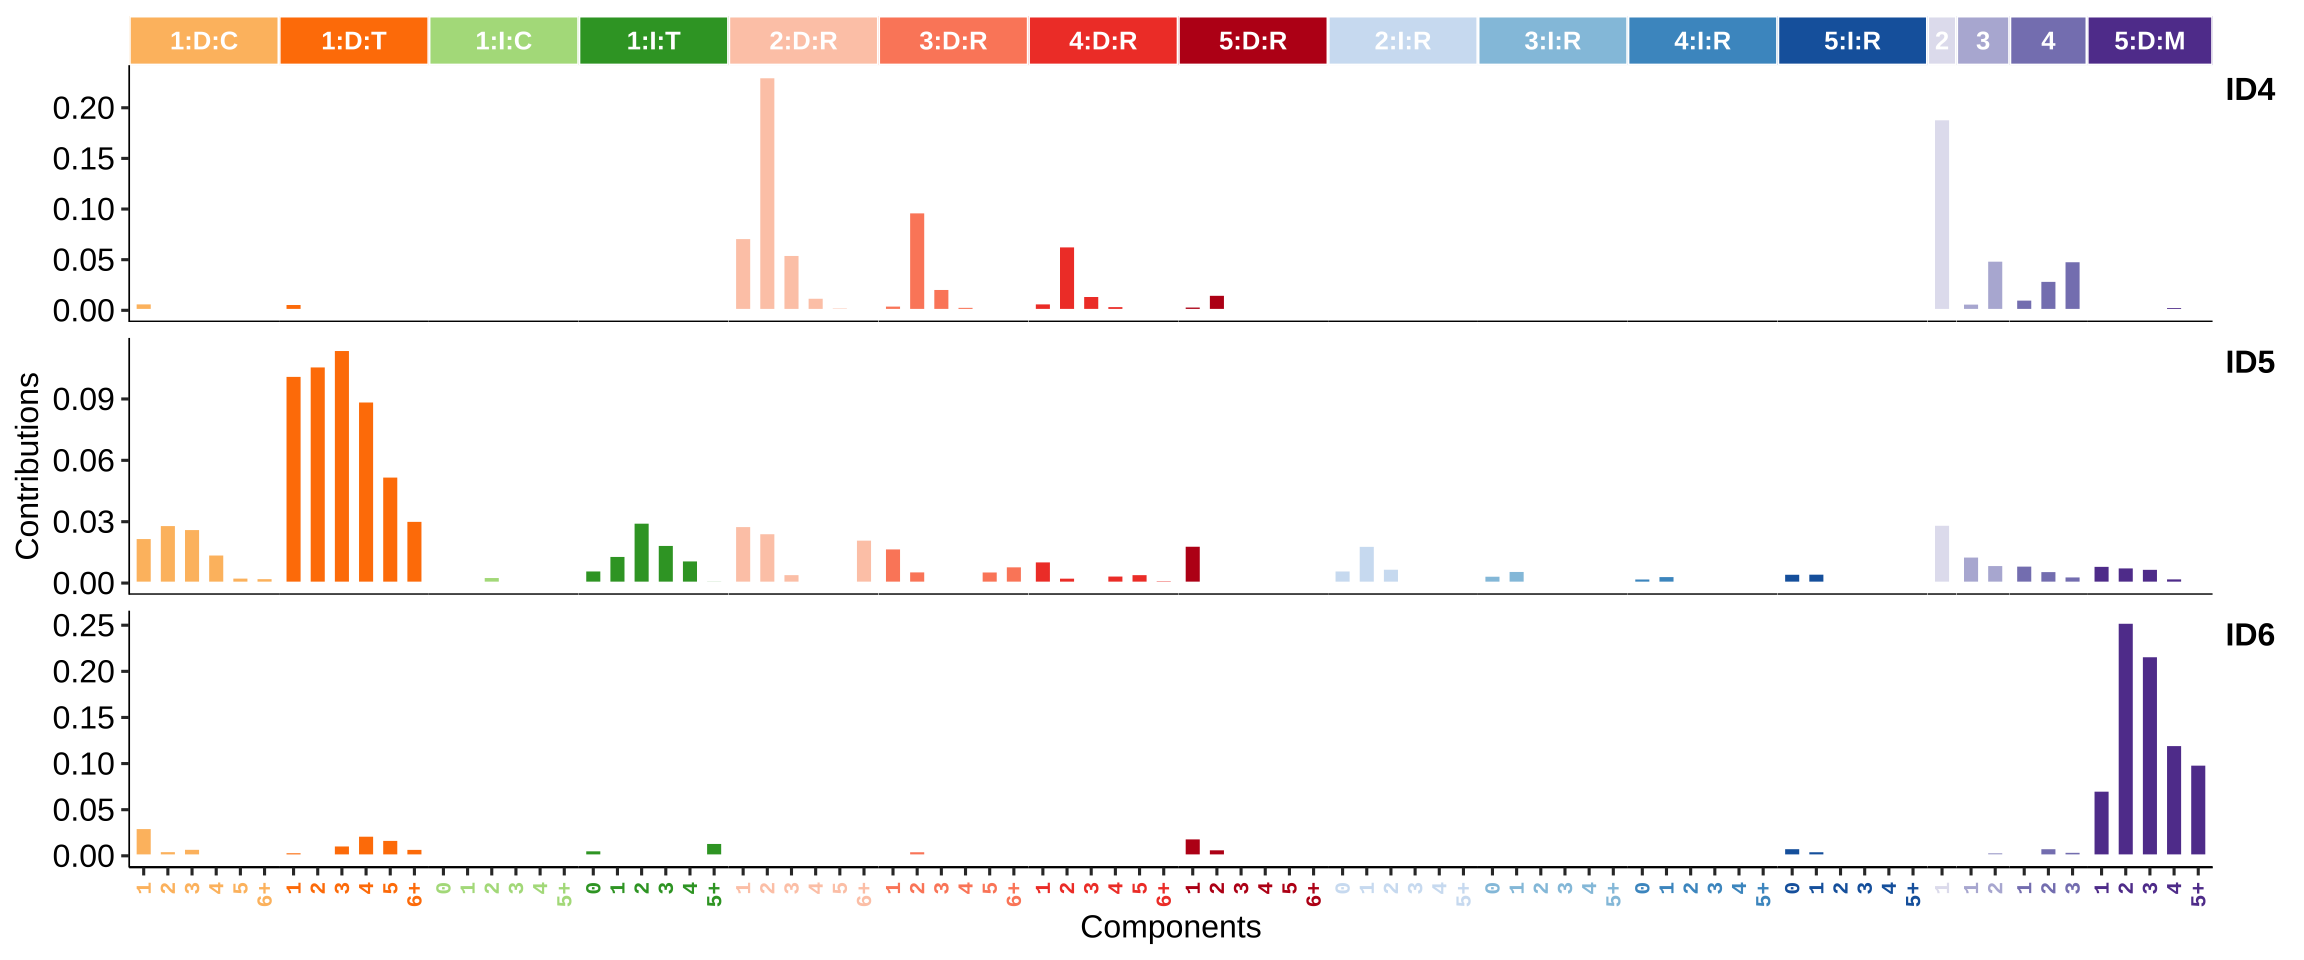
\includegraphics[width=0.95\linewidth]{sigminer_files/figure-latex/unnamed-chunk-82-1}

\hypertarget{exposure-activity-profile}{%
\subsection{Exposure (activity) profile}\label{exposure-activity-profile}}

\begin{Shaded}
\begin{Highlighting}[]
\FunctionTok{show\_sig\_exposure}\NormalTok{(mt\_sig)}
\end{Highlighting}
\end{Shaded}

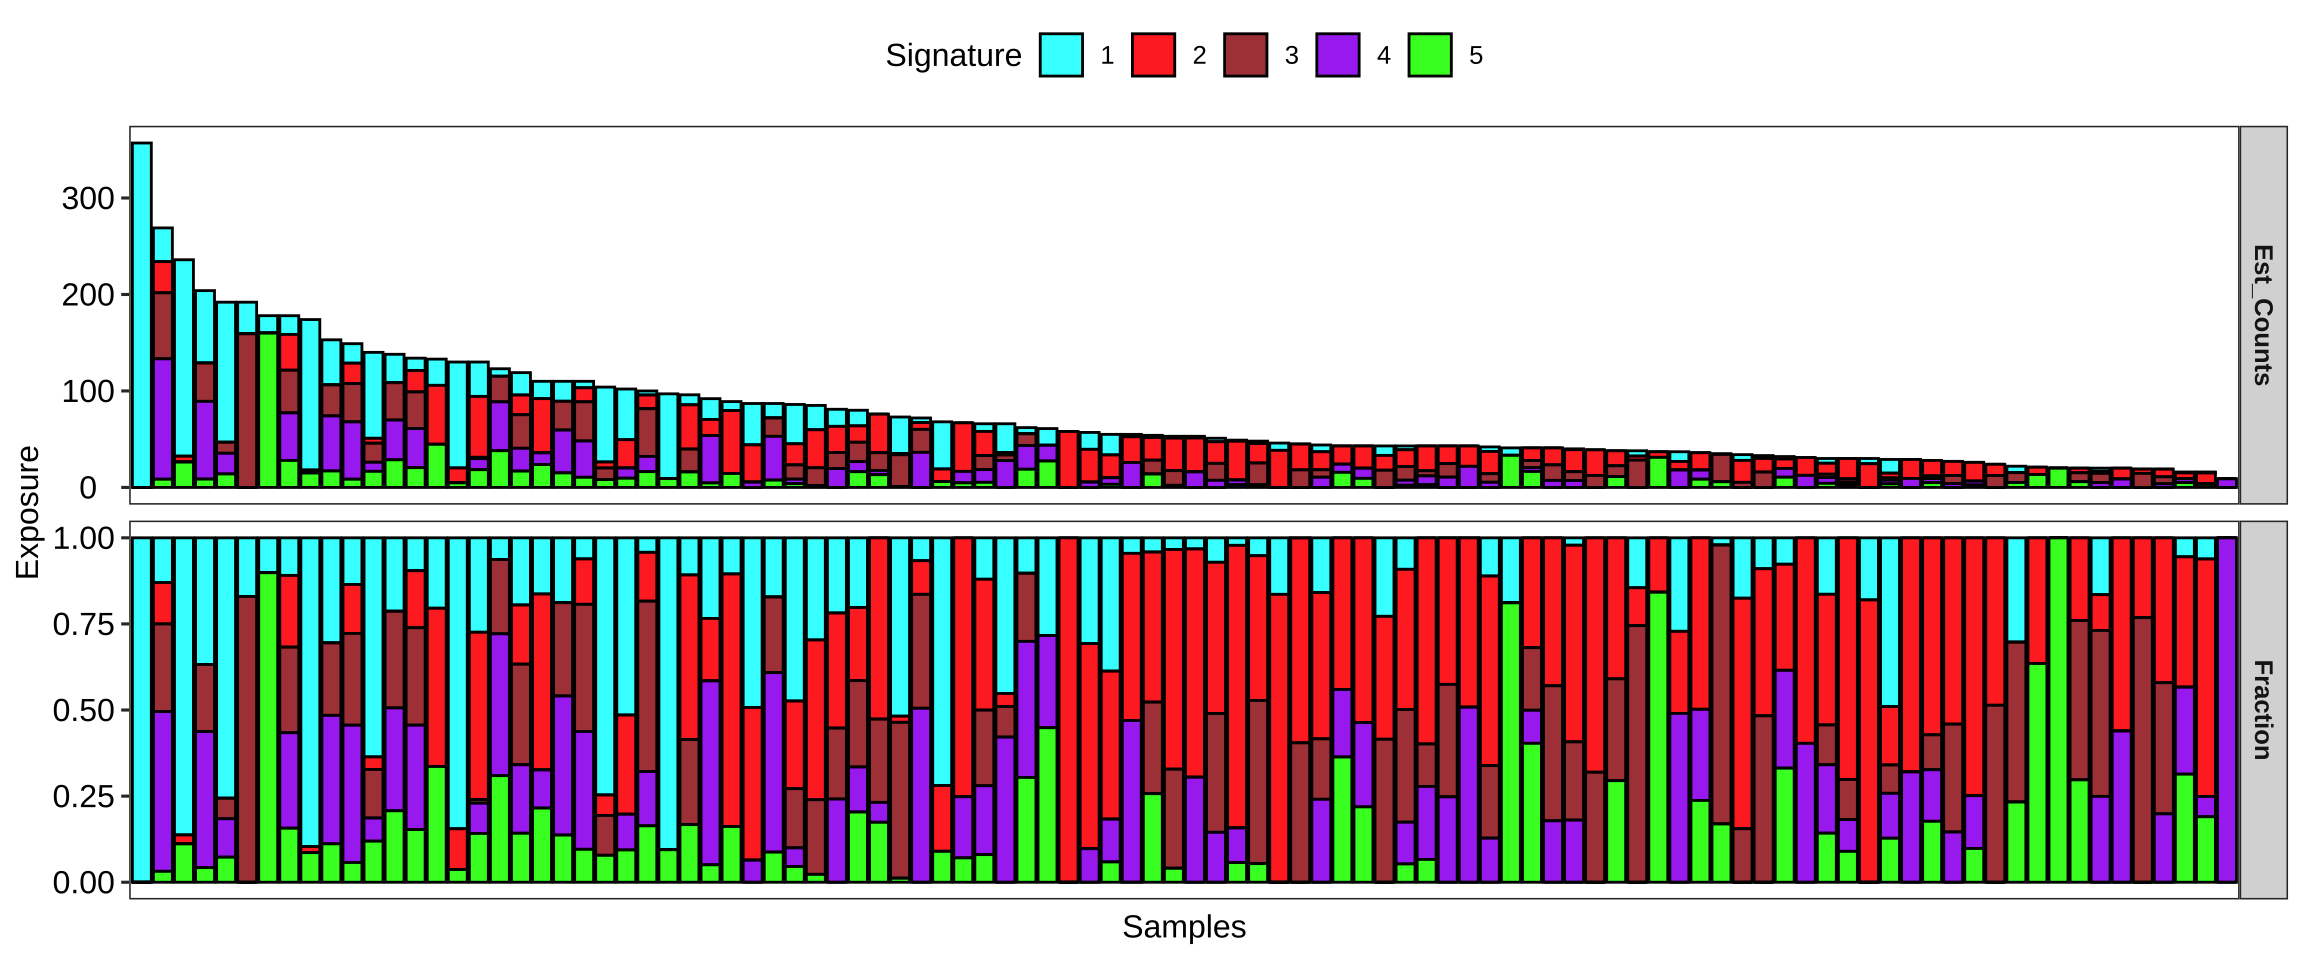
\includegraphics[width=0.95\linewidth]{sigminer_files/figure-latex/unnamed-chunk-83-1}

\begin{Shaded}
\begin{Highlighting}[]
\FunctionTok{show\_sig\_exposure}\NormalTok{(mt\_sig, }\AttributeTok{style =} \StringTok{"cosmic"}\NormalTok{)}
\end{Highlighting}
\end{Shaded}

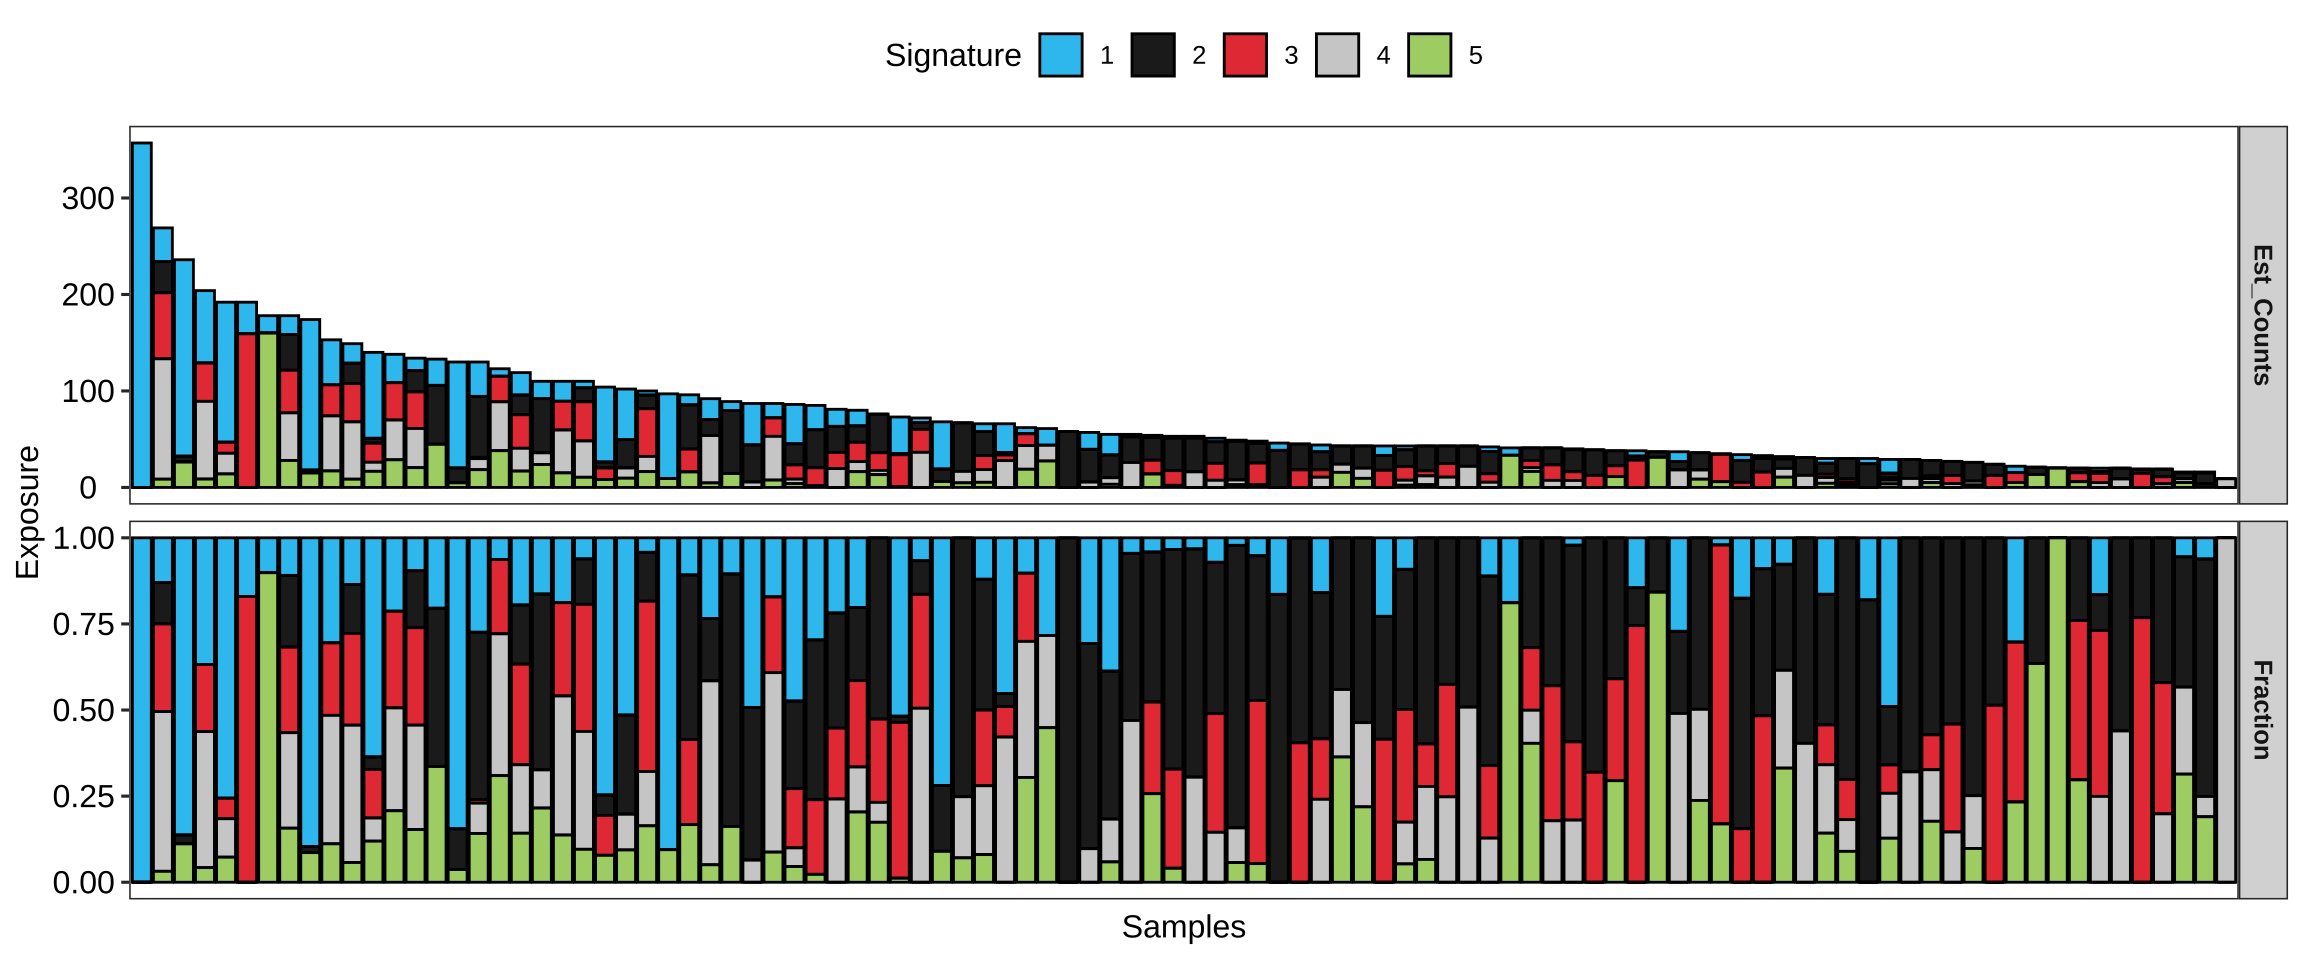
\includegraphics[width=0.95\linewidth]{sigminer_files/figure-latex/unnamed-chunk-84-1}

\begin{Shaded}
\begin{Highlighting}[]
\FunctionTok{show\_sig\_exposure}\NormalTok{(sig\_w, }\AttributeTok{style =} \StringTok{"cosmic"}\NormalTok{)}
\end{Highlighting}
\end{Shaded}

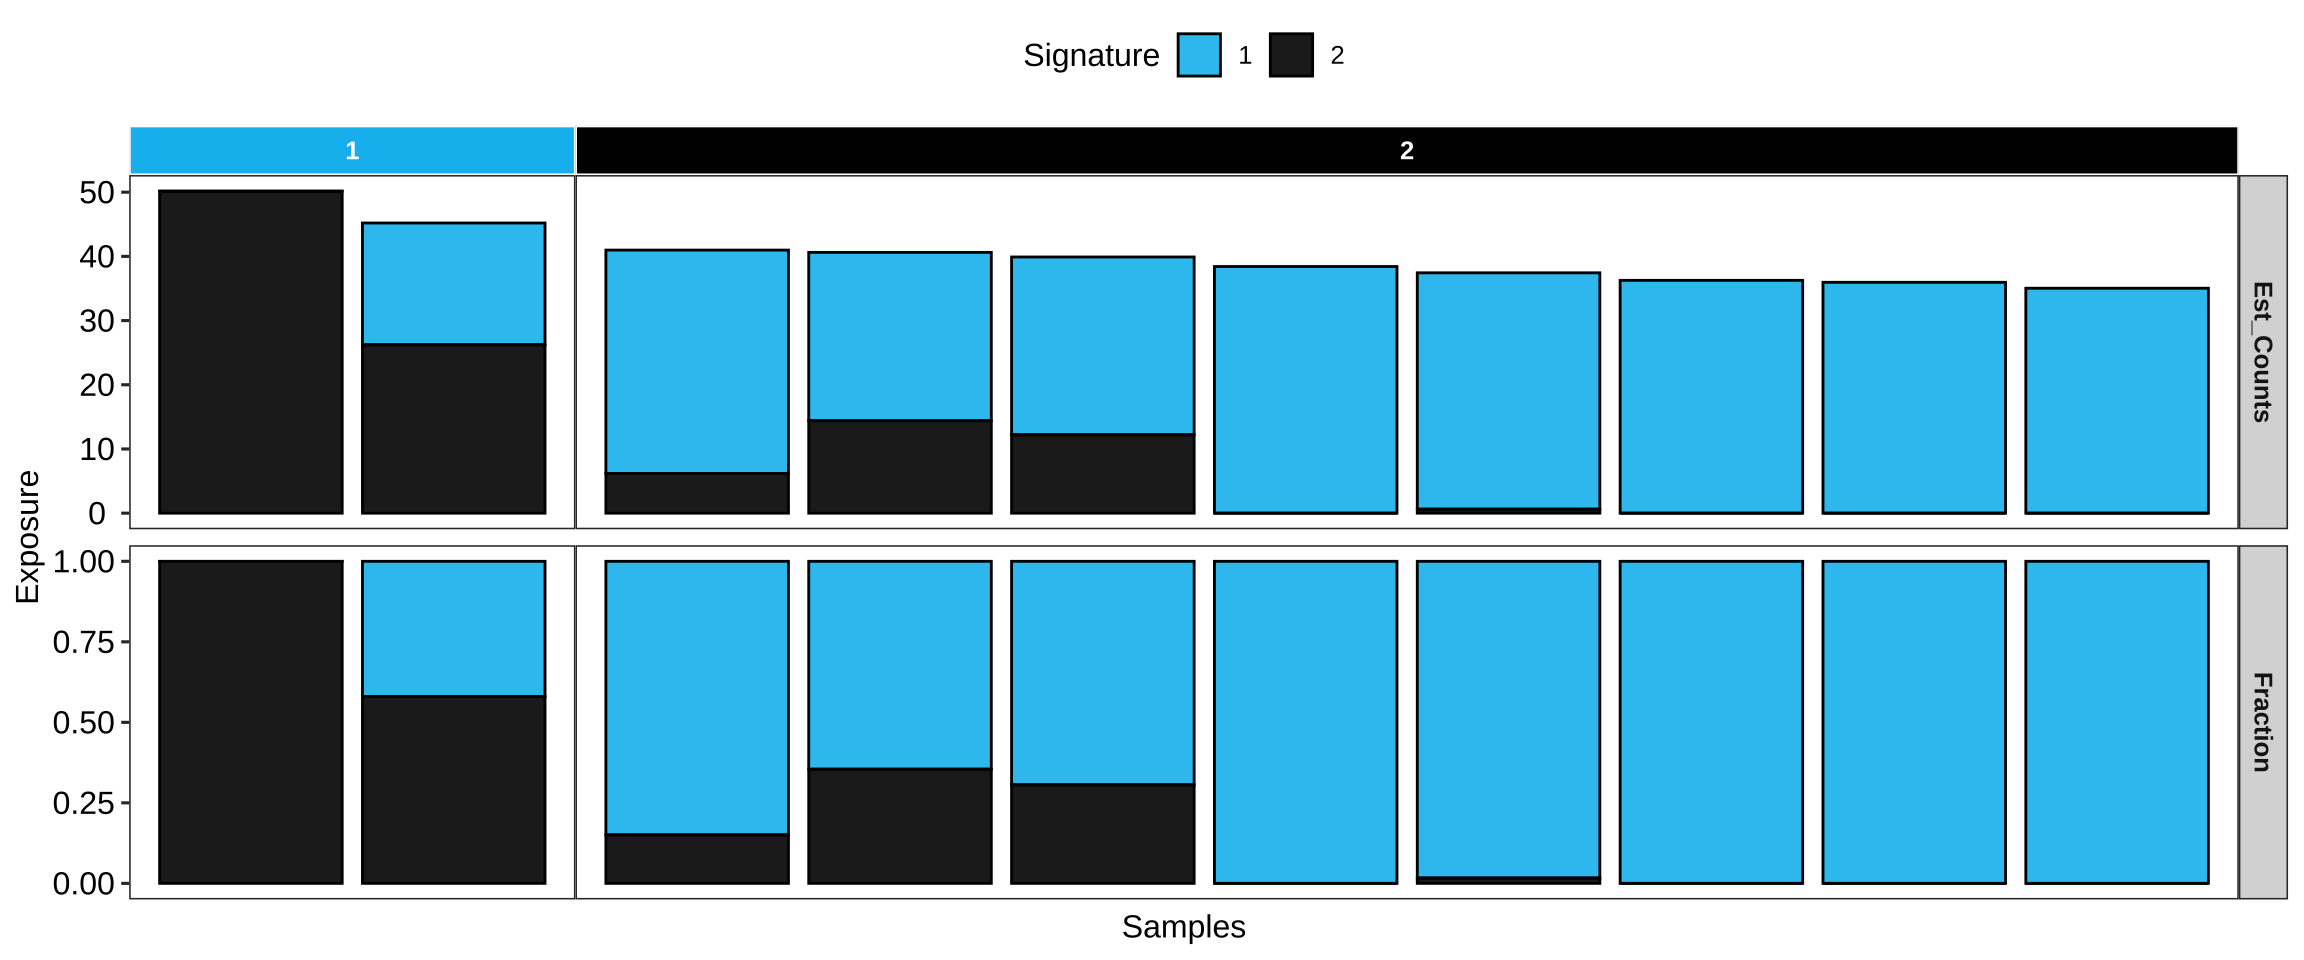
\includegraphics[width=0.95\linewidth]{sigminer_files/figure-latex/unnamed-chunk-85-1}

You can put group labels in the exposure profile.

\begin{Shaded}
\begin{Highlighting}[]
\NormalTok{grp }\OtherTok{\textless{}{-}} \FunctionTok{get\_groups}\NormalTok{(sig\_w)}
\DocumentationTok{\#\# i [2022{-}08{-}29 11:20:13]: Started.}
\DocumentationTok{\#\# v [2022{-}08{-}29 11:20:14]: \textquotesingle{}Signature\textquotesingle{} object detected.}
\DocumentationTok{\#\# i [2022{-}08{-}29 11:20:14]: Obtaining clusters from the hierarchical clustering of the consensus matrix...}
\DocumentationTok{\#\# i [2022{-}08{-}29 11:20:14]: Finding the dominant signature of each group...}
\DocumentationTok{\#\# =\textgreater{} Generating a table of group and dominant signature:}
\DocumentationTok{\#\#    }
\DocumentationTok{\#\#     Sig1 Sig2}
\DocumentationTok{\#\#   1    0    2}
\DocumentationTok{\#\#   2    8    0}
\DocumentationTok{\#\# =\textgreater{} Assigning a group to a signature with the maxium fraction (stored in \textquotesingle{}map\_table\textquotesingle{} attr)...}
\DocumentationTok{\#\# i [2022{-}08{-}29 11:20:14]: Summarizing...}
\DocumentationTok{\#\#  group \#1: 2 samples with Sig2 enriched.}
\DocumentationTok{\#\#  group \#2: 8 samples with Sig1 enriched.}
\DocumentationTok{\#\# ! [2022{-}08{-}29 11:20:14]: The \textquotesingle{}enrich\_sig\textquotesingle{} column is set to dominant signature in one group, please check and make it consistent with biological meaning (correct it by hand if necessary).}
\DocumentationTok{\#\# i [2022{-}08{-}29 11:20:14]: 0.236 secs elapsed.}
\NormalTok{grp\_label }\OtherTok{\textless{}{-}}\NormalTok{ grp}\SpecialCharTok{$}\NormalTok{group}
\FunctionTok{names}\NormalTok{(grp\_label) }\OtherTok{\textless{}{-}}\NormalTok{ grp}\SpecialCharTok{$}\NormalTok{sample}
\end{Highlighting}
\end{Shaded}

\begin{Shaded}
\begin{Highlighting}[]
\FunctionTok{show\_sig\_exposure}\NormalTok{(sig\_w, }\AttributeTok{style =} \StringTok{"cosmic"}\NormalTok{, }\AttributeTok{groups =}\NormalTok{ grp\_label)}
\end{Highlighting}
\end{Shaded}

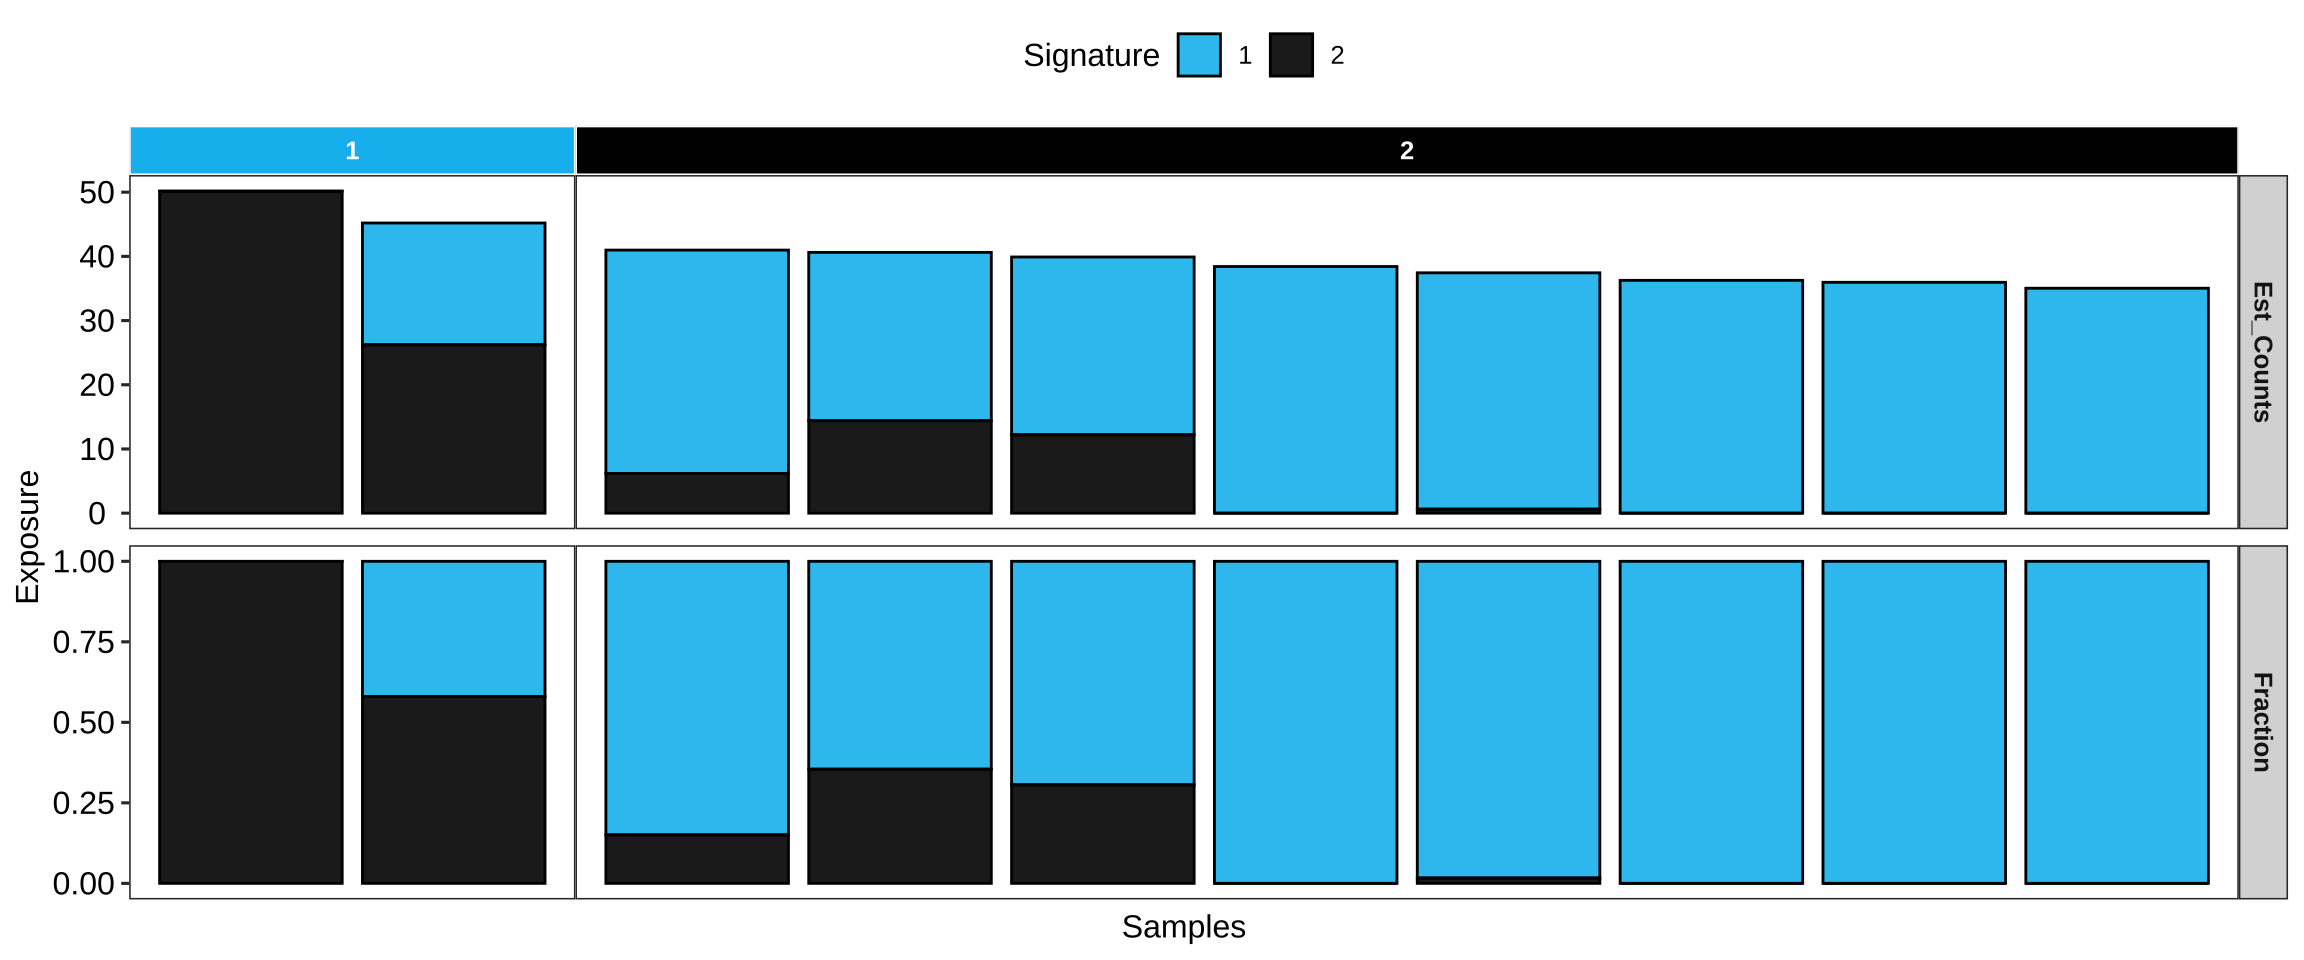
\includegraphics[width=0.95\linewidth]{sigminer_files/figure-latex/unnamed-chunk-87-1}

Of note:

\begin{itemize}
\tightlist
\item
  For COSMIC signatures, the absolute exposure is the estimated mutation counts.
\item
  For copy number signatures, the absolute exposure is the estimated copy number segments.
\end{itemize}

\hypertarget{consensus-map}{%
\subsection{Consensus map}\label{consensus-map}}

This can only support the result from \texttt{sig\_extract()} with multiple runs.

\begin{Shaded}
\begin{Highlighting}[]
\FunctionTok{show\_sig\_consensusmap}\NormalTok{(mt\_sig)}
\end{Highlighting}
\end{Shaded}

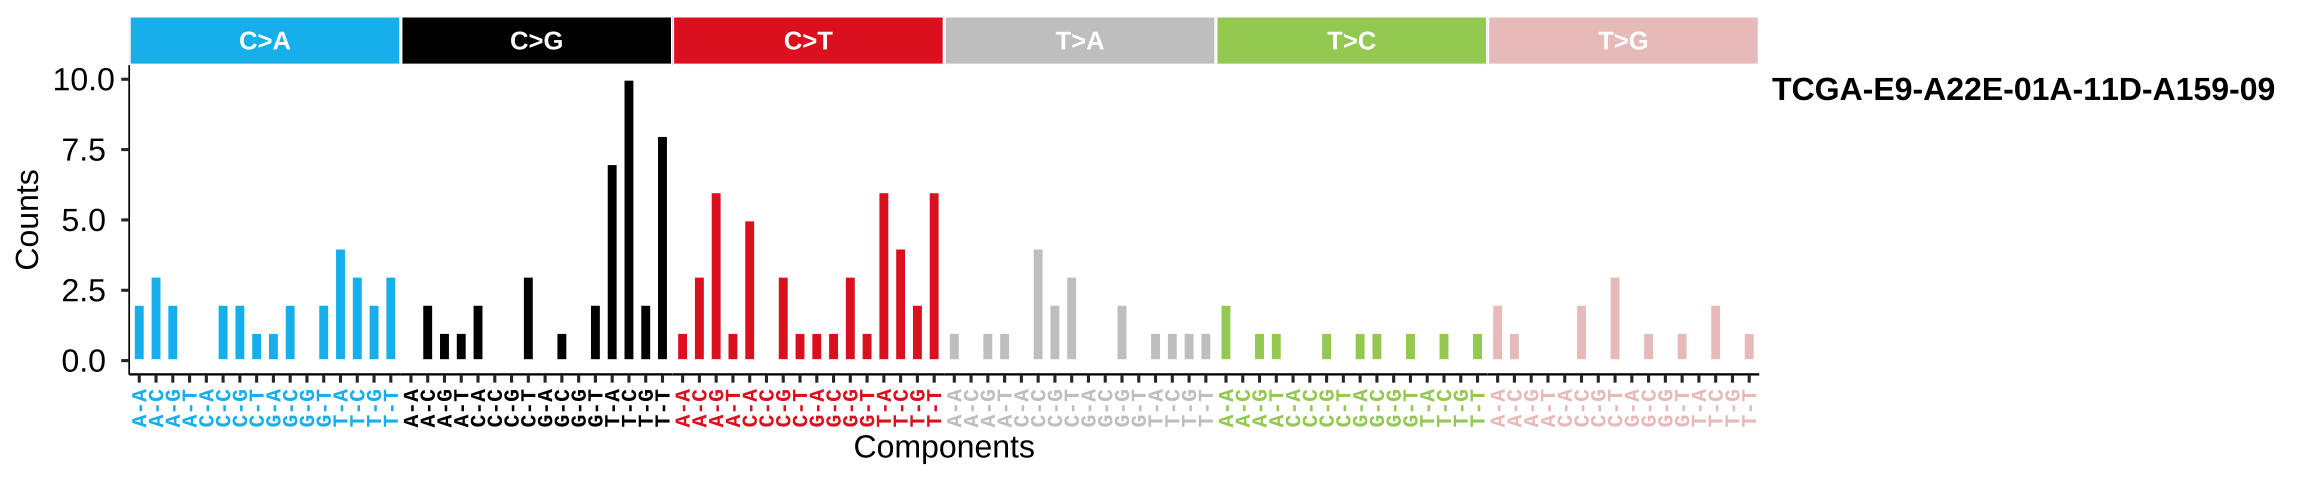
\includegraphics[width=0.95\linewidth]{sigminer_files/figure-latex/unnamed-chunk-88-1}

\hypertarget{catalogue-profile}{%
\subsection{Catalogue profile}\label{catalogue-profile}}

Based on plot method for signature, we can plot raw catalog profile.

\begin{Shaded}
\begin{Highlighting}[]
\FunctionTok{show\_catalogue}\NormalTok{(}\FunctionTok{t}\NormalTok{(mt\_tally}\SpecialCharTok{$}\NormalTok{nmf\_matrix), }\AttributeTok{style =} \StringTok{"cosmic"}\NormalTok{, }\AttributeTok{x\_label\_angle =} \DecValTok{90}\NormalTok{)}
\end{Highlighting}
\end{Shaded}

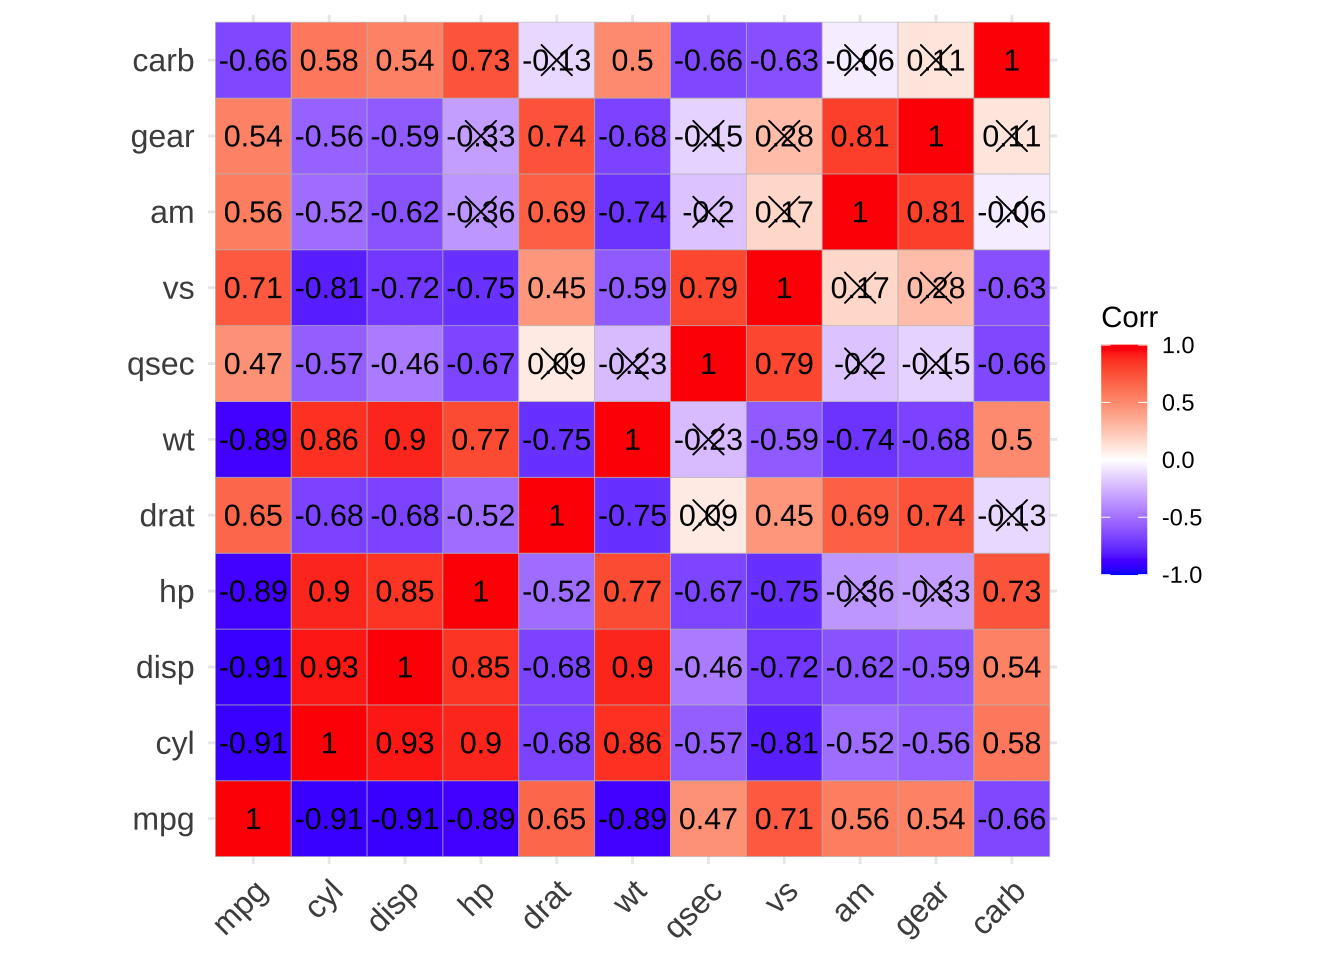
\includegraphics[width=0.95\linewidth]{sigminer_files/figure-latex/unnamed-chunk-89-1}

At default, the function sums all samples. Users can specify sample ID.

\begin{Shaded}
\begin{Highlighting}[]
\FunctionTok{show\_catalogue}\NormalTok{(}\FunctionTok{t}\NormalTok{(mt\_tally}\SpecialCharTok{$}\NormalTok{nmf\_matrix), }\AttributeTok{style =} \StringTok{"cosmic"}\NormalTok{, }\AttributeTok{samples =} \StringTok{"TCGA{-}E9{-}A22E{-}01A{-}11D{-}A159{-}09"}\NormalTok{, }\AttributeTok{x\_label\_angle =} \DecValTok{90}\NormalTok{)}
\end{Highlighting}
\end{Shaded}

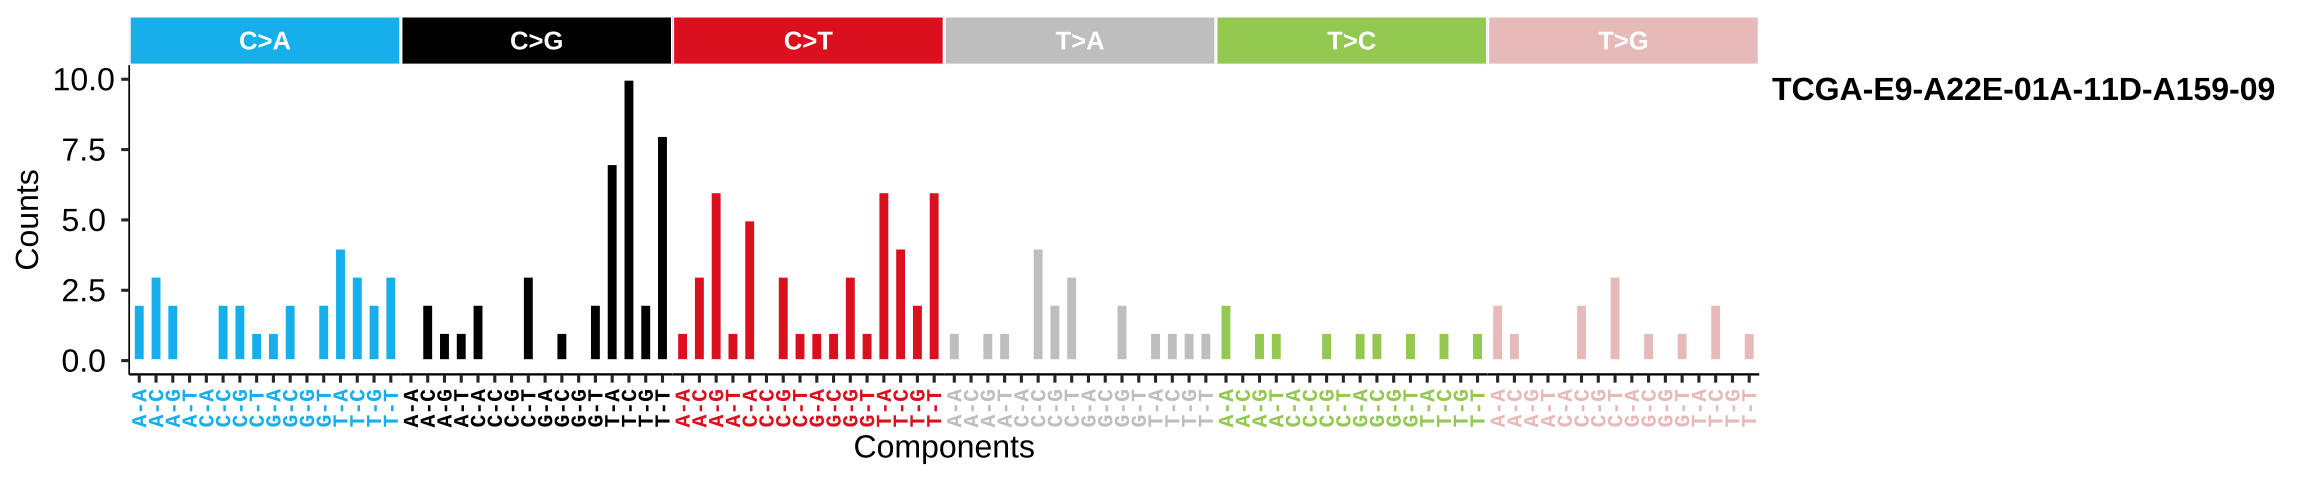
\includegraphics[width=0.95\linewidth]{sigminer_files/figure-latex/unnamed-chunk-90-1}

\hypertarget{part-part-iii-miscellaneous-topics}{%
\part*{Part III: Miscellaneous topics}\label{part-part-iii-miscellaneous-topics}}
\addcontentsline{toc}{part}{Part III: Miscellaneous topics}

\hypertarget{universal-analysis}{%
\chapter{Universal analysis}\label{universal-analysis}}

\hypertarget{association-analysis-and-visualization}{%
\section{Association analysis and visualization}\label{association-analysis-and-visualization}}

\hypertarget{general-numeric-association}{%
\subsection{General numeric association}\label{general-numeric-association}}

For general numeric association, you can use \texttt{show\_cor()} function.

\begin{Shaded}
\begin{Highlighting}[]
\FunctionTok{data}\NormalTok{(}\StringTok{"mtcars"}\NormalTok{)}
\NormalTok{p1 }\OtherTok{\textless{}{-}} \FunctionTok{show\_cor}\NormalTok{(mtcars)}
\NormalTok{p2 }\OtherTok{\textless{}{-}} \FunctionTok{show\_cor}\NormalTok{(mtcars,}
  \AttributeTok{x\_vars =} \FunctionTok{colnames}\NormalTok{(mtcars)[}\DecValTok{1}\SpecialCharTok{:}\DecValTok{4}\NormalTok{],}
  \AttributeTok{y\_vars =} \FunctionTok{colnames}\NormalTok{(mtcars)[}\DecValTok{5}\SpecialCharTok{:}\DecValTok{8}\NormalTok{]}
\NormalTok{)}
\NormalTok{p3 }\OtherTok{\textless{}{-}} \FunctionTok{show\_cor}\NormalTok{(mtcars, }\AttributeTok{vis\_method =} \StringTok{"circle"}\NormalTok{, }\AttributeTok{p\_adj =} \StringTok{"fdr"}\NormalTok{)}
\NormalTok{p1}
\end{Highlighting}
\end{Shaded}

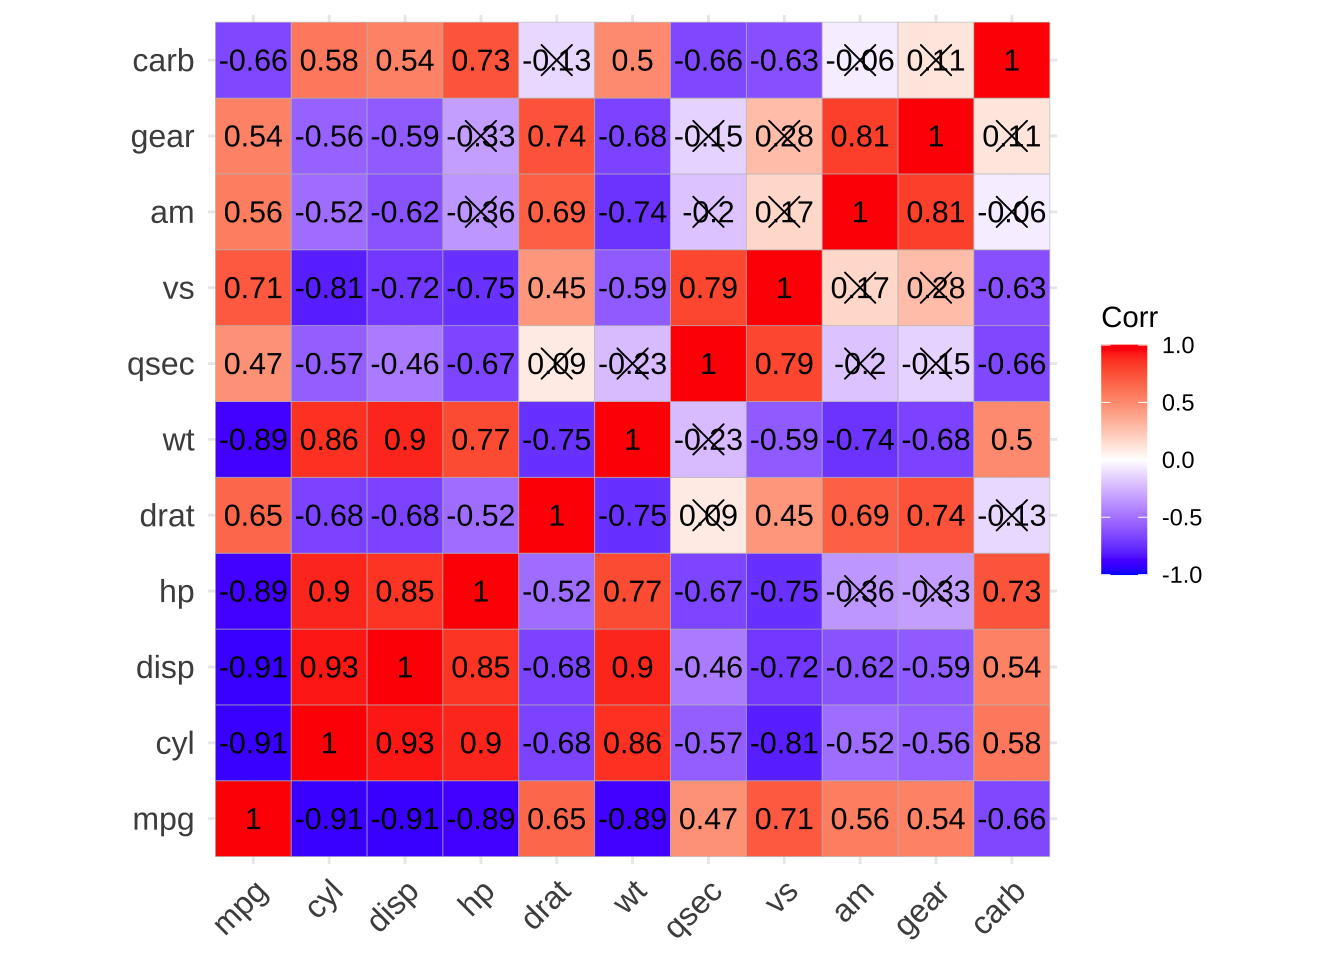
\includegraphics[width=0.95\linewidth]{sigminer_files/figure-latex/unnamed-chunk-91-1}

\begin{Shaded}
\begin{Highlighting}[]
\NormalTok{p1}\SpecialCharTok{$}\NormalTok{cor}
\DocumentationTok{\#\# $cor\_mat}
\DocumentationTok{\#\#        mpg   cyl  disp    hp  drat    wt  qsec    vs    am  gear  carb}
\DocumentationTok{\#\# mpg   1.00 {-}0.91 {-}0.91 {-}0.89  0.65 {-}0.89  0.47  0.71  0.56  0.54 {-}0.66}
\DocumentationTok{\#\# cyl  {-}0.91  1.00  0.93  0.90 {-}0.68  0.86 {-}0.57 {-}0.81 {-}0.52 {-}0.56  0.58}
\DocumentationTok{\#\# disp {-}0.91  0.93  1.00  0.85 {-}0.68  0.90 {-}0.46 {-}0.72 {-}0.62 {-}0.59  0.54}
\DocumentationTok{\#\# hp   {-}0.89  0.90  0.85  1.00 {-}0.52  0.77 {-}0.67 {-}0.75 {-}0.36 {-}0.33  0.73}
\DocumentationTok{\#\# drat  0.65 {-}0.68 {-}0.68 {-}0.52  1.00 {-}0.75  0.09  0.45  0.69  0.74 {-}0.13}
\DocumentationTok{\#\# wt   {-}0.89  0.86  0.90  0.77 {-}0.75  1.00 {-}0.23 {-}0.59 {-}0.74 {-}0.68  0.50}
\DocumentationTok{\#\# qsec  0.47 {-}0.57 {-}0.46 {-}0.67  0.09 {-}0.23  1.00  0.79 {-}0.20 {-}0.15 {-}0.66}
\DocumentationTok{\#\# vs    0.71 {-}0.81 {-}0.72 {-}0.75  0.45 {-}0.59  0.79  1.00  0.17  0.28 {-}0.63}
\DocumentationTok{\#\# am    0.56 {-}0.52 {-}0.62 {-}0.36  0.69 {-}0.74 {-}0.20  0.17  1.00  0.81 {-}0.06}
\DocumentationTok{\#\# gear  0.54 {-}0.56 {-}0.59 {-}0.33  0.74 {-}0.68 {-}0.15  0.28  0.81  1.00  0.11}
\DocumentationTok{\#\# carb {-}0.66  0.58  0.54  0.73 {-}0.13  0.50 {-}0.66 {-}0.63 {-}0.06  0.11  1.00}
\DocumentationTok{\#\# }
\DocumentationTok{\#\# $p\_mat}
\DocumentationTok{\#\#               mpg          cyl         disp           hp         drat}
\DocumentationTok{\#\# mpg  0.000000e+00 6.112687e{-}10 9.380327e{-}10 1.787835e{-}07 1.776240e{-}05}
\DocumentationTok{\#\# cyl  6.112687e{-}10 0.000000e+00 1.802838e{-}12 3.477861e{-}09 8.244636e{-}06}
\DocumentationTok{\#\# disp 9.380327e{-}10 1.802838e{-}12 0.000000e+00 7.142679e{-}08 5.282022e{-}06}
\DocumentationTok{\#\# hp   1.787835e{-}07 3.477861e{-}09 7.142679e{-}08 0.000000e+00 9.988772e{-}03}
\DocumentationTok{\#\# drat 1.776240e{-}05 8.244636e{-}06 5.282022e{-}06 9.988772e{-}03 0.000000e+00}
\DocumentationTok{\#\# wt   1.293959e{-}10 1.217567e{-}07 1.222320e{-}11 4.145827e{-}05 4.784260e{-}06}
\DocumentationTok{\#\# qsec 1.708199e{-}02 3.660533e{-}04 1.314404e{-}02 5.766253e{-}06 6.195826e{-}01}
\DocumentationTok{\#\# vs   3.415937e{-}05 1.843018e{-}08 5.235012e{-}06 2.940896e{-}06 1.167553e{-}02}
\DocumentationTok{\#\# am   2.850207e{-}04 2.151207e{-}03 3.662114e{-}04 1.798309e{-}01 4.726790e{-}06}
\DocumentationTok{\#\# gear 5.400948e{-}03 4.173297e{-}03 9.635921e{-}04 4.930119e{-}01 8.360110e{-}06}
\DocumentationTok{\#\# carb 1.084446e{-}03 1.942340e{-}03 2.526789e{-}02 7.827810e{-}07 6.211834e{-}01}
\DocumentationTok{\#\#                wt         qsec           vs           am         gear}
\DocumentationTok{\#\# mpg  1.293959e{-}10 1.708199e{-}02 3.415937e{-}05 2.850207e{-}04 5.400948e{-}03}
\DocumentationTok{\#\# cyl  1.217567e{-}07 3.660533e{-}04 1.843018e{-}08 2.151207e{-}03 4.173297e{-}03}
\DocumentationTok{\#\# disp 1.222320e{-}11 1.314404e{-}02 5.235012e{-}06 3.662114e{-}04 9.635921e{-}04}
\DocumentationTok{\#\# hp   4.145827e{-}05 5.766253e{-}06 2.940896e{-}06 1.798309e{-}01 4.930119e{-}01}
\DocumentationTok{\#\# drat 4.784260e{-}06 6.195826e{-}01 1.167553e{-}02 4.726790e{-}06 8.360110e{-}06}
\DocumentationTok{\#\# wt   0.000000e+00 3.388683e{-}01 9.798492e{-}04 1.125440e{-}05 4.586601e{-}04}
\DocumentationTok{\#\# qsec 3.388683e{-}01 0.000000e+00 1.029669e{-}06 2.056621e{-}01 2.425344e{-}01}
\DocumentationTok{\#\# vs   9.798492e{-}04 1.029669e{-}06 0.000000e+00 3.570439e{-}01 2.579439e{-}01}
\DocumentationTok{\#\# am   1.125440e{-}05 2.056621e{-}01 3.570439e{-}01 0.000000e+00 5.834043e{-}08}
\DocumentationTok{\#\# gear 4.586601e{-}04 2.425344e{-}01 2.579439e{-}01 5.834043e{-}08 0.000000e+00}
\DocumentationTok{\#\# carb 1.463861e{-}02 4.536949e{-}05 6.670496e{-}04 7.544526e{-}01 1.290291e{-}01}
\DocumentationTok{\#\#              carb}
\DocumentationTok{\#\# mpg  1.084446e{-}03}
\DocumentationTok{\#\# cyl  1.942340e{-}03}
\DocumentationTok{\#\# disp 2.526789e{-}02}
\DocumentationTok{\#\# hp   7.827810e{-}07}
\DocumentationTok{\#\# drat 6.211834e{-}01}
\DocumentationTok{\#\# wt   1.463861e{-}02}
\DocumentationTok{\#\# qsec 4.536949e{-}05}
\DocumentationTok{\#\# vs   6.670496e{-}04}
\DocumentationTok{\#\# am   7.544526e{-}01}
\DocumentationTok{\#\# gear 1.290291e{-}01}
\DocumentationTok{\#\# carb 0.000000e+00}
\NormalTok{p2}
\end{Highlighting}
\end{Shaded}

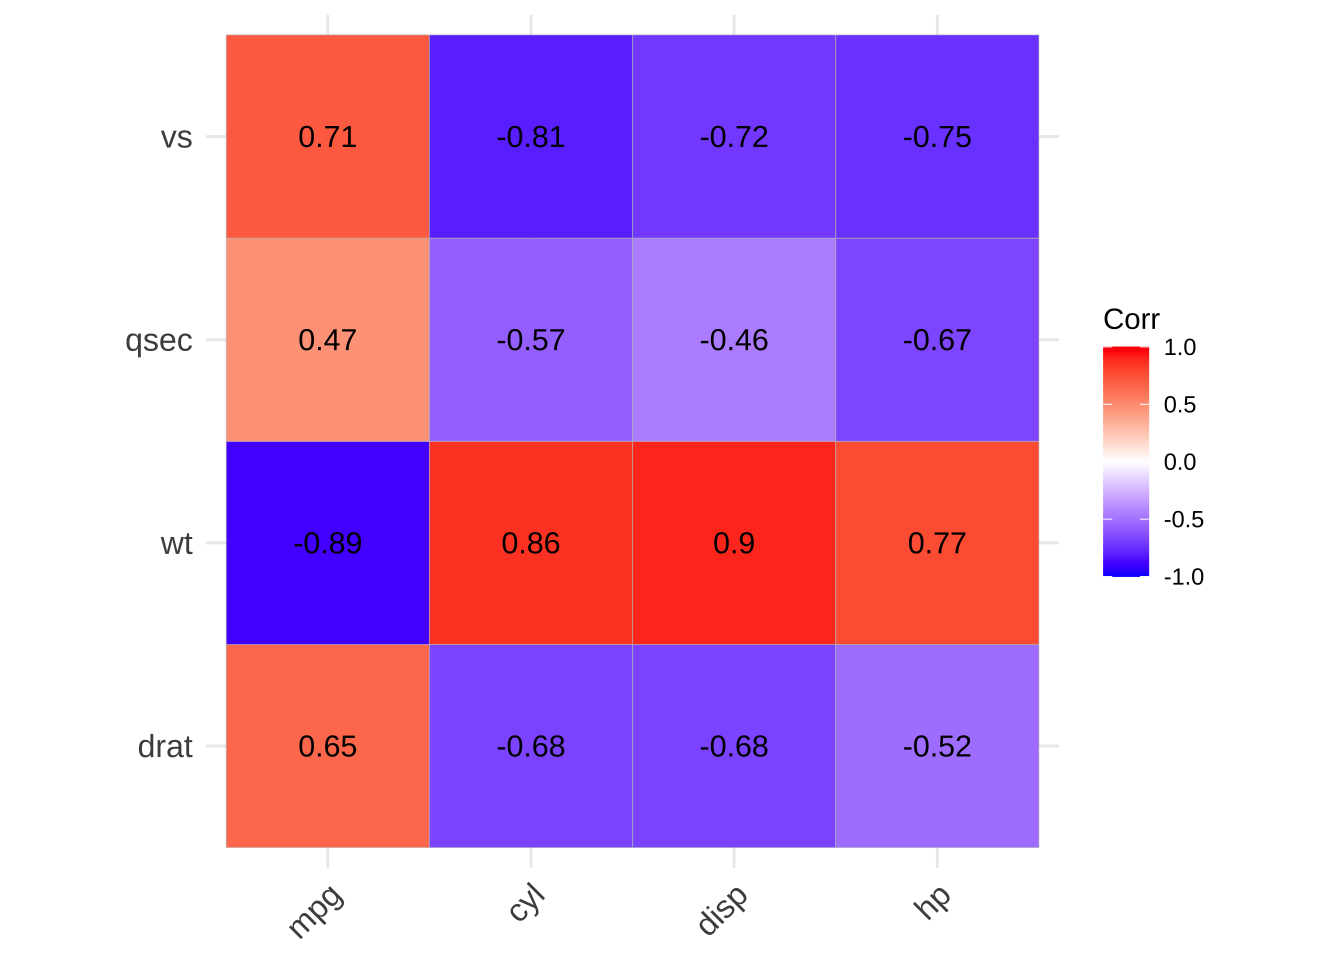
\includegraphics[width=0.95\linewidth]{sigminer_files/figure-latex/unnamed-chunk-91-2}

\begin{Shaded}
\begin{Highlighting}[]
\NormalTok{p3}
\end{Highlighting}
\end{Shaded}

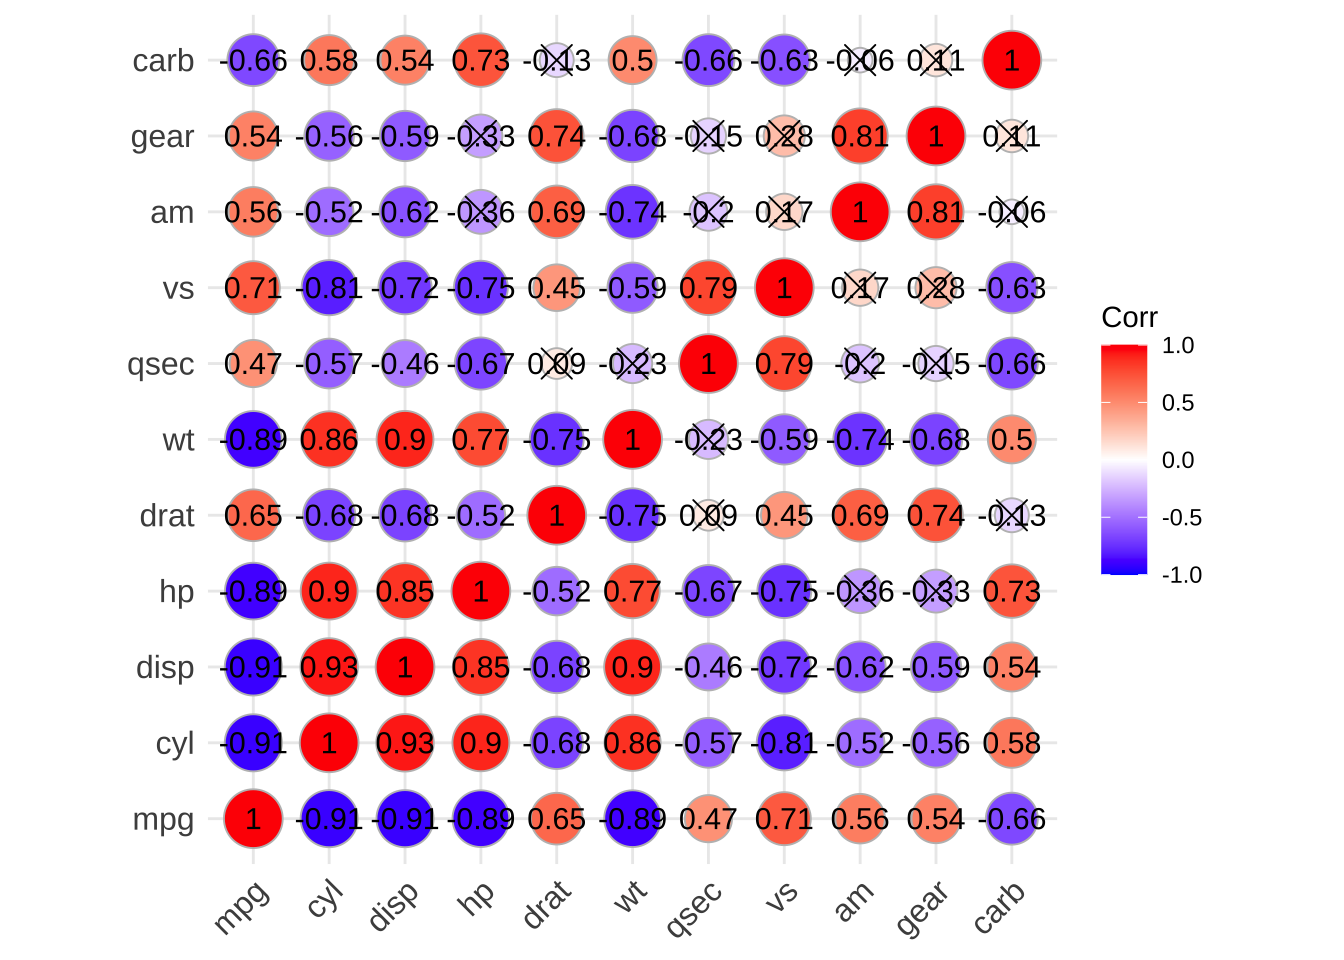
\includegraphics[width=0.95\linewidth]{sigminer_files/figure-latex/unnamed-chunk-91-3}

\hypertarget{comprehensive-association}{%
\subsection{Comprehensive association}\label{comprehensive-association}}

For comprehensive association analysis including both continuous and categorical variables,
there are several functions available in \textbf{sigminer}:

\begin{itemize}
\tightlist
\item
  \texttt{get\_sig\_feature\_association()}.
\item
  \texttt{get\_tidy\_association()}.
\item
  \texttt{show\_sig\_feature\_corrplot()}.
\end{itemize}

Currently, I haven't provided a proper example dataset for showing usage of all functions above (please read their documentation), here only the tidy dataset from our study \citep{wang2021copy} is given to show the plot function.

\begin{Shaded}
\begin{Highlighting}[]
\CommentTok{\# The data is generated from Wang, Shixiang et al.}
\FunctionTok{load}\NormalTok{(}\FunctionTok{system.file}\NormalTok{(}\StringTok{"extdata"}\NormalTok{, }\StringTok{"asso\_data.RData"}\NormalTok{,}
  \AttributeTok{package =} \StringTok{"sigminer"}\NormalTok{, }\AttributeTok{mustWork =} \ConstantTok{TRUE}
\NormalTok{))}
\NormalTok{p }\OtherTok{\textless{}{-}} \FunctionTok{show\_sig\_feature\_corrplot}\NormalTok{(tidy\_data.seqz.feature, }\AttributeTok{p\_val =} \FloatTok{0.05}\NormalTok{)}
\NormalTok{p}
\end{Highlighting}
\end{Shaded}

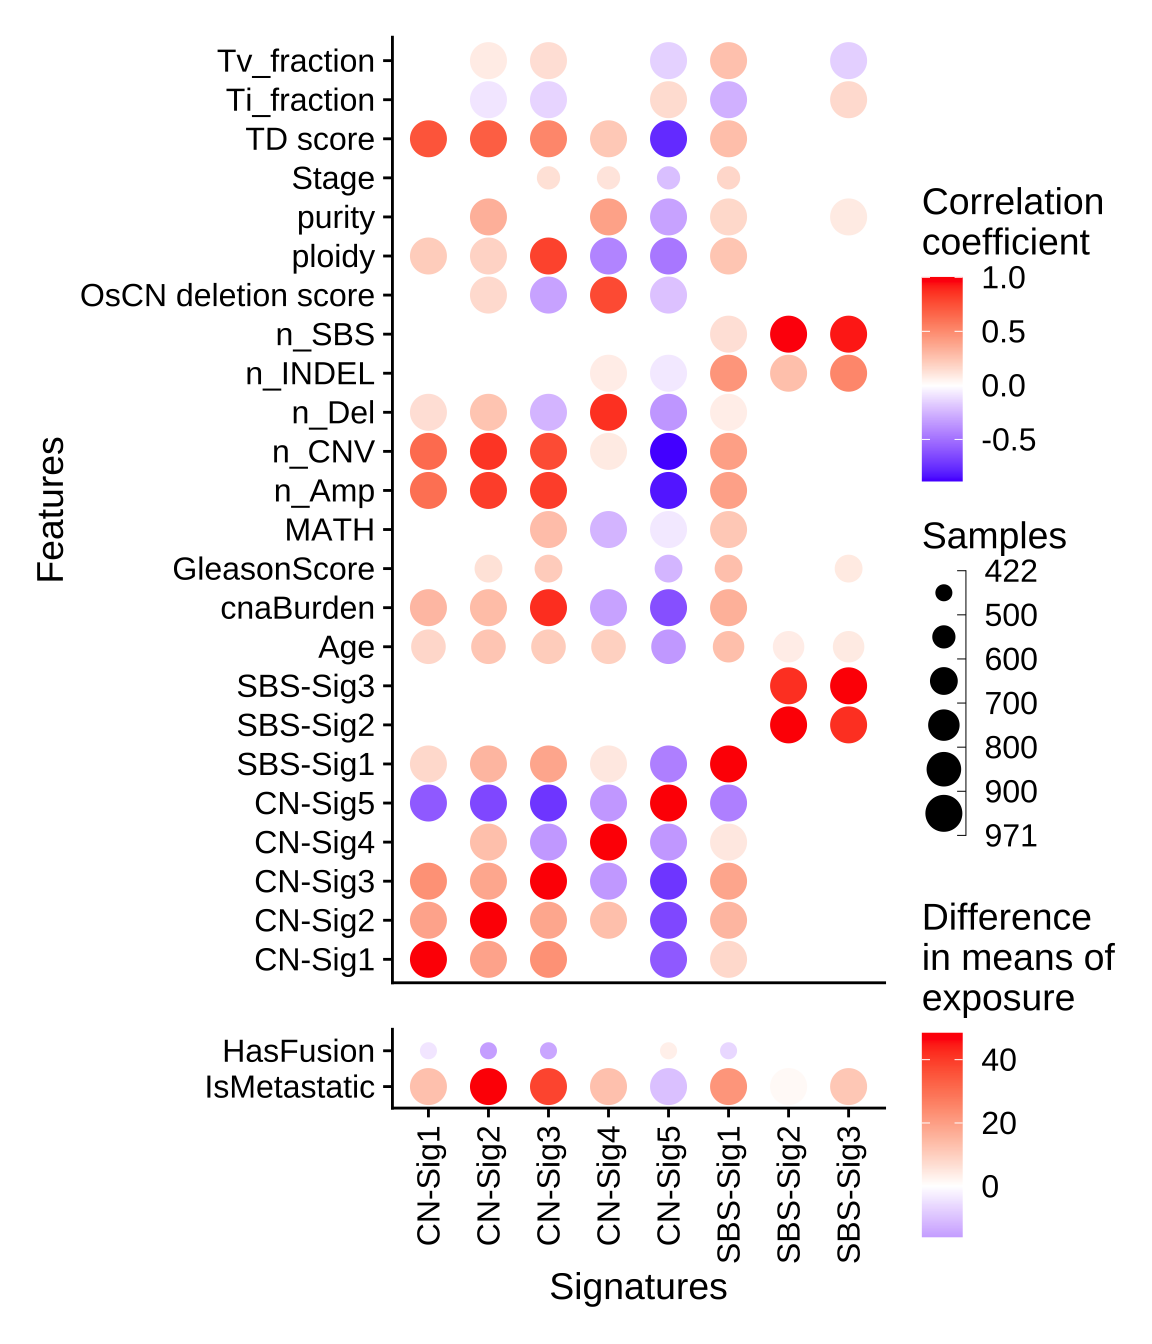
\includegraphics[width=0.95\linewidth]{sigminer_files/figure-latex/unnamed-chunk-92-1}

\hypertarget{group-analysis-and-visualization}{%
\section{Group Analysis and Visualization}\label{group-analysis-and-visualization}}

Group analysis is a common task in cancer study. \textbf{Sigminer} supports dividing samples into multiple groups and comparing genotype/phenotype feature measures.

\hypertarget{group-generation}{%
\subsection{Group Generation}\label{group-generation}}

There are multiple methods to generate groups, including `consensus' (default, can be only used by result from \texttt{sig\_extract()}), `k-means' etc. After determining groups, \textbf{sigminer} will assign each group to a signature with maximum fraction. We may say a group is \texttt{Sig\_x} enriched.

\begin{Shaded}
\begin{Highlighting}[]
\FunctionTok{data}\NormalTok{(}\StringTok{"simulated\_catalogs"}\NormalTok{)}
\NormalTok{mt\_sig }\OtherTok{\textless{}{-}} \FunctionTok{sig\_extract}\NormalTok{(}\FunctionTok{t}\NormalTok{(simulated\_catalogs}\SpecialCharTok{$}\NormalTok{set1), }\AttributeTok{n\_sig =} \DecValTok{10}\NormalTok{, }\AttributeTok{nrun =} \DecValTok{3}\NormalTok{)}
\DocumentationTok{\#\# NMF algorithm: \textquotesingle{}brunet\textquotesingle{}}
\DocumentationTok{\#\# Multiple runs: 3}
\DocumentationTok{\#\# Mode: sequential [foreach:doParallelMC]}
\DocumentationTok{\#\# Runs: |                                                        Runs: |                                                  |   0\%Runs: |                                                        Runs: |============                                      |  25\%Runs: |                                                        Runs: |=========================                         |  50\%Runs: |                                                        Runs: |======================================            |  75\%Runs: |                                                        Runs: |==================================================| 100\%}
\DocumentationTok{\#\# System time:}
\DocumentationTok{\#\#    user  system elapsed }
\DocumentationTok{\#\#   6.242   0.072   6.387}
\end{Highlighting}
\end{Shaded}

\begin{Shaded}
\begin{Highlighting}[]
\NormalTok{mt\_grps }\OtherTok{\textless{}{-}} \FunctionTok{get\_groups}\NormalTok{(mt\_sig, }\AttributeTok{method =} \StringTok{"consensus"}\NormalTok{, }\AttributeTok{match\_consensus =} \ConstantTok{TRUE}\NormalTok{)}
\DocumentationTok{\#\# i [2022{-}08{-}29 11:20:31]: Started.}
\DocumentationTok{\#\# v [2022{-}08{-}29 11:20:31]: \textquotesingle{}Signature\textquotesingle{} object detected.}
\DocumentationTok{\#\# i [2022{-}08{-}29 11:20:31]: Obtaining clusters from the hierarchical clustering of the consensus matrix...}
\DocumentationTok{\#\# i [2022{-}08{-}29 11:20:31]: Finding the dominant signature of each group...}
\DocumentationTok{\#\# =\textgreater{} Generating a table of group and dominant signature:}
\DocumentationTok{\#\#     }
\DocumentationTok{\#\#      Sig1 Sig10 Sig2 Sig3 Sig4 Sig5 Sig7 Sig8 Sig9}
\DocumentationTok{\#\#   1     0     2    0    2    0    0    0    0    0}
\DocumentationTok{\#\#   10    1     0    0    1    0    4    0    0    0}
\DocumentationTok{\#\#   2     0     0    1    0    0    0    0    0    0}
\DocumentationTok{\#\#   3     1     0    0    0    0    0    0    0    0}
\DocumentationTok{\#\#   4     1     0    1    0    2    0    0    0    0}
\DocumentationTok{\#\#   5     0     0    0    0    0    0    0    1    0}
\DocumentationTok{\#\#   6     1     0    1    0    0    0    2    0    0}
\DocumentationTok{\#\#   7     0     0    0    0    0    0    0    0    3}
\DocumentationTok{\#\#   8     0     0    1    4    0    0    0    0    0}
\DocumentationTok{\#\#   9     1     0    0    0    0    0    0    0    0}
\DocumentationTok{\#\# =\textgreater{} Assigning a group to a signature with the maxium fraction (stored in \textquotesingle{}map\_table\textquotesingle{} attr)...}
\DocumentationTok{\#\# i [2022{-}08{-}29 11:20:31]: Summarizing...}
\DocumentationTok{\#\#  group \#1: 4 samples with Sig10 enriched.}
\DocumentationTok{\#\#  group \#10: 6 samples with Sig5 enriched.}
\DocumentationTok{\#\#  group \#2: 1 samples with Sig2 enriched.}
\DocumentationTok{\#\#  group \#3: 1 samples with Sig1 enriched.}
\DocumentationTok{\#\#  group \#4: 4 samples with Sig4 enriched.}
\DocumentationTok{\#\#  group \#5: 1 samples with Sig8 enriched.}
\DocumentationTok{\#\#  group \#6: 4 samples with Sig7 enriched.}
\DocumentationTok{\#\#  group \#7: 3 samples with Sig9 enriched.}
\DocumentationTok{\#\#  group \#8: 5 samples with Sig3 enriched.}
\DocumentationTok{\#\#  group \#9: 1 samples with Sig1 enriched.}
\DocumentationTok{\#\# ! [2022{-}08{-}29 11:20:31]: The \textquotesingle{}enrich\_sig\textquotesingle{} column is set to dominant signature in one group, please check and make it consistent with biological meaning (correct it by hand if necessary).}
\DocumentationTok{\#\# i [2022{-}08{-}29 11:20:31]: 0.083 secs elapsed.}
\FunctionTok{head}\NormalTok{(mt\_grps)}
\DocumentationTok{\#\#       sample group silhouette\_width enrich\_sig}
\DocumentationTok{\#\# 1: Sample\_14     1         6.67e{-}01      Sig10}
\DocumentationTok{\#\# 2:  Sample\_6     1         0.00e+00      Sig10}
\DocumentationTok{\#\# 3:  Sample\_2     1         1.00e+00      Sig10}
\DocumentationTok{\#\# 4:  Sample\_5     1         0.00e+00      Sig10}
\DocumentationTok{\#\# 5: Sample\_22     2         1.00e+00       Sig2}
\DocumentationTok{\#\# 6: Sample\_12     3         1.67e{-}16       Sig1}
\end{Highlighting}
\end{Shaded}

The returned sample orders match sample orders in clustered consensus matrix.

\begin{Shaded}
\begin{Highlighting}[]
\FunctionTok{show\_sig\_consensusmap}\NormalTok{(mt\_sig)}
\end{Highlighting}
\end{Shaded}

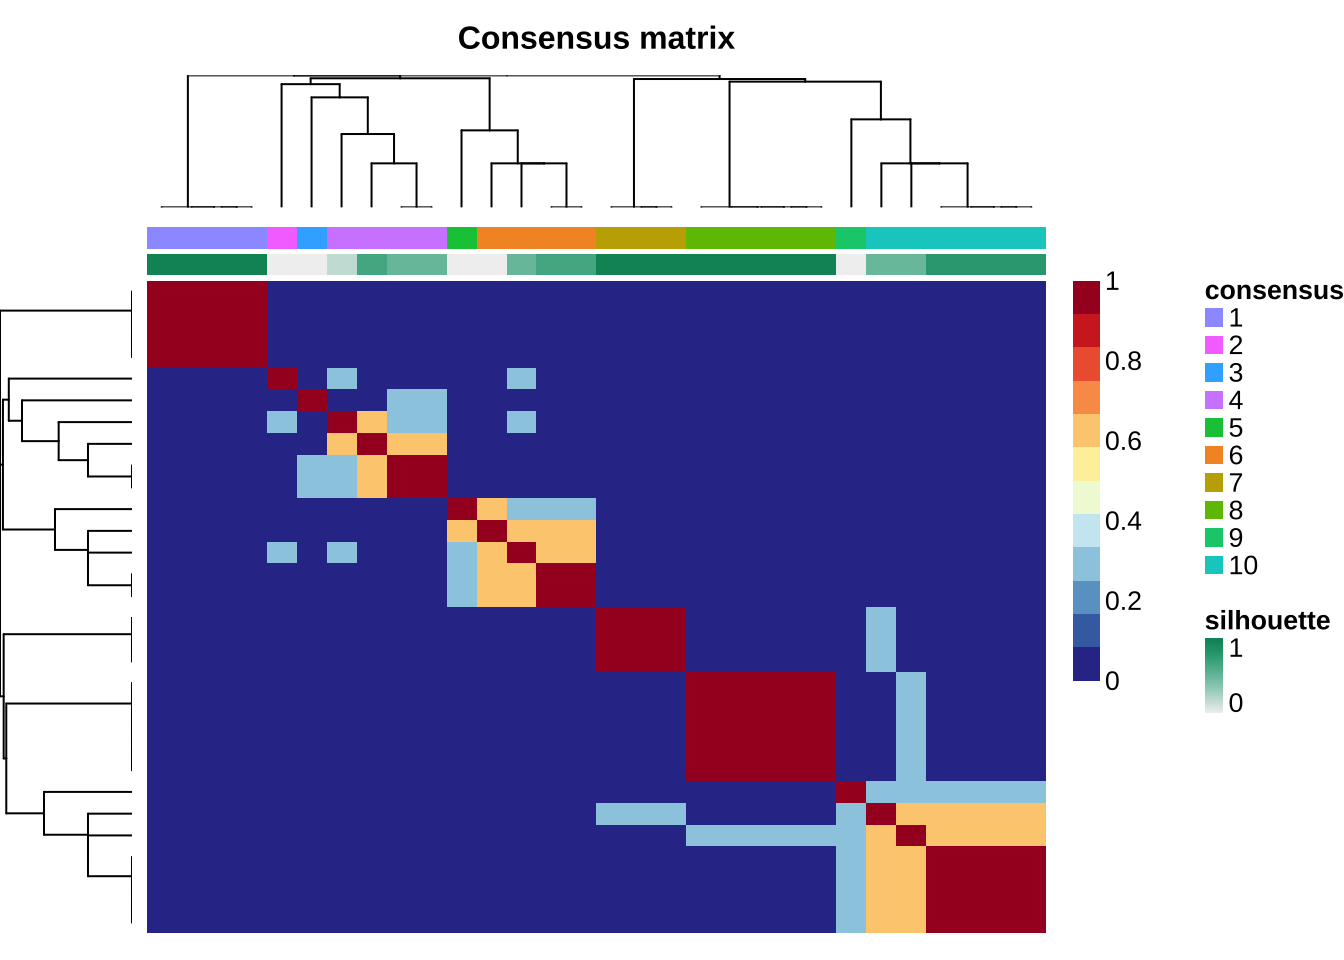
\includegraphics[width=0.95\linewidth]{sigminer_files/figure-latex/unnamed-chunk-95-1}

Sometimes, the mapping between groups and enriched signatures may not right. Users should check it and even correct it manually.

\begin{Shaded}
\begin{Highlighting}[]
\FunctionTok{attr}\NormalTok{(mt\_grps, }\StringTok{"map\_table"}\NormalTok{)}
\DocumentationTok{\#\#     }
\DocumentationTok{\#\#      Sig1 Sig10 Sig2 Sig3 Sig4 Sig5 Sig7 Sig8 Sig9}
\DocumentationTok{\#\#   1     0     2    0    2    0    0    0    0    0}
\DocumentationTok{\#\#   10    1     0    0    1    0    4    0    0    0}
\DocumentationTok{\#\#   2     0     0    1    0    0    0    0    0    0}
\DocumentationTok{\#\#   3     1     0    0    0    0    0    0    0    0}
\DocumentationTok{\#\#   4     1     0    1    0    2    0    0    0    0}
\DocumentationTok{\#\#   5     0     0    0    0    0    0    0    1    0}
\DocumentationTok{\#\#   6     1     0    1    0    0    0    2    0    0}
\DocumentationTok{\#\#   7     0     0    0    0    0    0    0    0    3}
\DocumentationTok{\#\#   8     0     0    1    4    0    0    0    0    0}
\DocumentationTok{\#\#   9     1     0    0    0    0    0    0    0    0}
\end{Highlighting}
\end{Shaded}

\hypertarget{group-comparison-analysis}{%
\subsection{Group Comparison Analysis}\label{group-comparison-analysis}}

\begin{Shaded}
\begin{Highlighting}[]
\FunctionTok{load}\NormalTok{(}\FunctionTok{system.file}\NormalTok{(}\StringTok{"extdata"}\NormalTok{, }\StringTok{"toy\_copynumber\_signature\_by\_W.RData"}\NormalTok{,}
  \AttributeTok{package =} \StringTok{"sigminer"}\NormalTok{, }\AttributeTok{mustWork =} \ConstantTok{TRUE}
\NormalTok{))}
\CommentTok{\# Assign samples to clusters}
\NormalTok{groups }\OtherTok{\textless{}{-}} \FunctionTok{get\_groups}\NormalTok{(sig, }\AttributeTok{method =} \StringTok{"k{-}means"}\NormalTok{)}
\DocumentationTok{\#\# i [2022{-}08{-}29 11:20:33]: Started.}
\DocumentationTok{\#\# v [2022{-}08{-}29 11:20:33]: \textquotesingle{}Signature\textquotesingle{} object detected.}
\DocumentationTok{\#\# i [2022{-}08{-}29 11:20:33]: Running k{-}means with 2 clusters...}
\DocumentationTok{\#\# i [2022{-}08{-}29 11:20:33]: Generating a table of group and signature contribution (stored in \textquotesingle{}map\_table\textquotesingle{} attr):}
\DocumentationTok{\#\#        Sig1      Sig2}
\DocumentationTok{\#\# 1 0.2097559 0.7901116}
\DocumentationTok{\#\# 2 0.8964984 0.1035016}
\DocumentationTok{\#\# i [2022{-}08{-}29 11:20:33]: Assigning a group to a signature with the maximum fraction...}
\DocumentationTok{\#\# i [2022{-}08{-}29 11:20:33]: Summarizing...}
\DocumentationTok{\#\#  group \#1: 2 samples with Sig2 enriched.}
\DocumentationTok{\#\#  group \#2: 8 samples with Sig1 enriched.}
\DocumentationTok{\#\# ! [2022{-}08{-}29 11:20:33]: The \textquotesingle{}enrich\_sig\textquotesingle{} column is set to dominant signature in one group, please check and make it consistent with biological meaning (correct it by hand if necessary).}
\DocumentationTok{\#\# i [2022{-}08{-}29 11:20:33]: 0.036 secs elapsed.}
\FunctionTok{set.seed}\NormalTok{(}\DecValTok{1234}\NormalTok{)}
\NormalTok{groups}\SpecialCharTok{$}\NormalTok{prob }\OtherTok{\textless{}{-}} \FunctionTok{rnorm}\NormalTok{(}\DecValTok{10}\NormalTok{)}
\NormalTok{groups}\SpecialCharTok{$}\NormalTok{new\_group }\OtherTok{\textless{}{-}} \FunctionTok{sample}\NormalTok{(}\FunctionTok{c}\NormalTok{(}\StringTok{"1"}\NormalTok{, }\StringTok{"2"}\NormalTok{, }\StringTok{"3"}\NormalTok{, }\StringTok{"4"}\NormalTok{, }\ConstantTok{NA}\NormalTok{), }\AttributeTok{size =} \FunctionTok{nrow}\NormalTok{(groups), }\AttributeTok{replace =} \ConstantTok{TRUE}\NormalTok{)}
\CommentTok{\# Compare groups (filter NAs for categorical coloumns)}
\NormalTok{groups.cmp }\OtherTok{\textless{}{-}} \FunctionTok{get\_group\_comparison}\NormalTok{(groups[, }\SpecialCharTok{{-}}\DecValTok{1}\NormalTok{],}
  \AttributeTok{col\_group =} \StringTok{"group"}\NormalTok{,}
  \AttributeTok{cols\_to\_compare =} \FunctionTok{c}\NormalTok{(}\StringTok{"prob"}\NormalTok{, }\StringTok{"new\_group"}\NormalTok{),}
  \AttributeTok{type =} \FunctionTok{c}\NormalTok{(}\StringTok{"co"}\NormalTok{, }\StringTok{"ca"}\NormalTok{), }\AttributeTok{verbose =} \ConstantTok{TRUE}
\NormalTok{)}
\DocumentationTok{\#\# Treat prob as continuous variable.}
\DocumentationTok{\#\# Treat new\_group as categorical variable.}
\CommentTok{\# Compare groups (Set NAs of categorical columns to \textquotesingle{}Rest\textquotesingle{})}
\NormalTok{groups.cmp2 }\OtherTok{\textless{}{-}} \FunctionTok{get\_group\_comparison}\NormalTok{(groups[, }\SpecialCharTok{{-}}\DecValTok{1}\NormalTok{],}
  \AttributeTok{col\_group =} \StringTok{"group"}\NormalTok{,}
  \AttributeTok{cols\_to\_compare =} \FunctionTok{c}\NormalTok{(}\StringTok{"prob"}\NormalTok{, }\StringTok{"new\_group"}\NormalTok{),}
  \AttributeTok{type =} \FunctionTok{c}\NormalTok{(}\StringTok{"co"}\NormalTok{, }\StringTok{"ca"}\NormalTok{), }\AttributeTok{NAs =} \StringTok{"Rest"}\NormalTok{, }\AttributeTok{verbose =} \ConstantTok{TRUE}
\NormalTok{)}
\DocumentationTok{\#\# Treat prob as continuous variable.}
\DocumentationTok{\#\# Treat new\_group as categorical variable.}
\end{Highlighting}
\end{Shaded}

\hypertarget{group-visualization}{%
\subsection{Group Visualization}\label{group-visualization}}

\begin{Shaded}
\begin{Highlighting}[]
\NormalTok{ggcomp }\OtherTok{\textless{}{-}} \FunctionTok{show\_group\_comparison}\NormalTok{(groups.cmp2)}
\NormalTok{ggcomp}\SpecialCharTok{$}\NormalTok{co\_comb}
\end{Highlighting}
\end{Shaded}

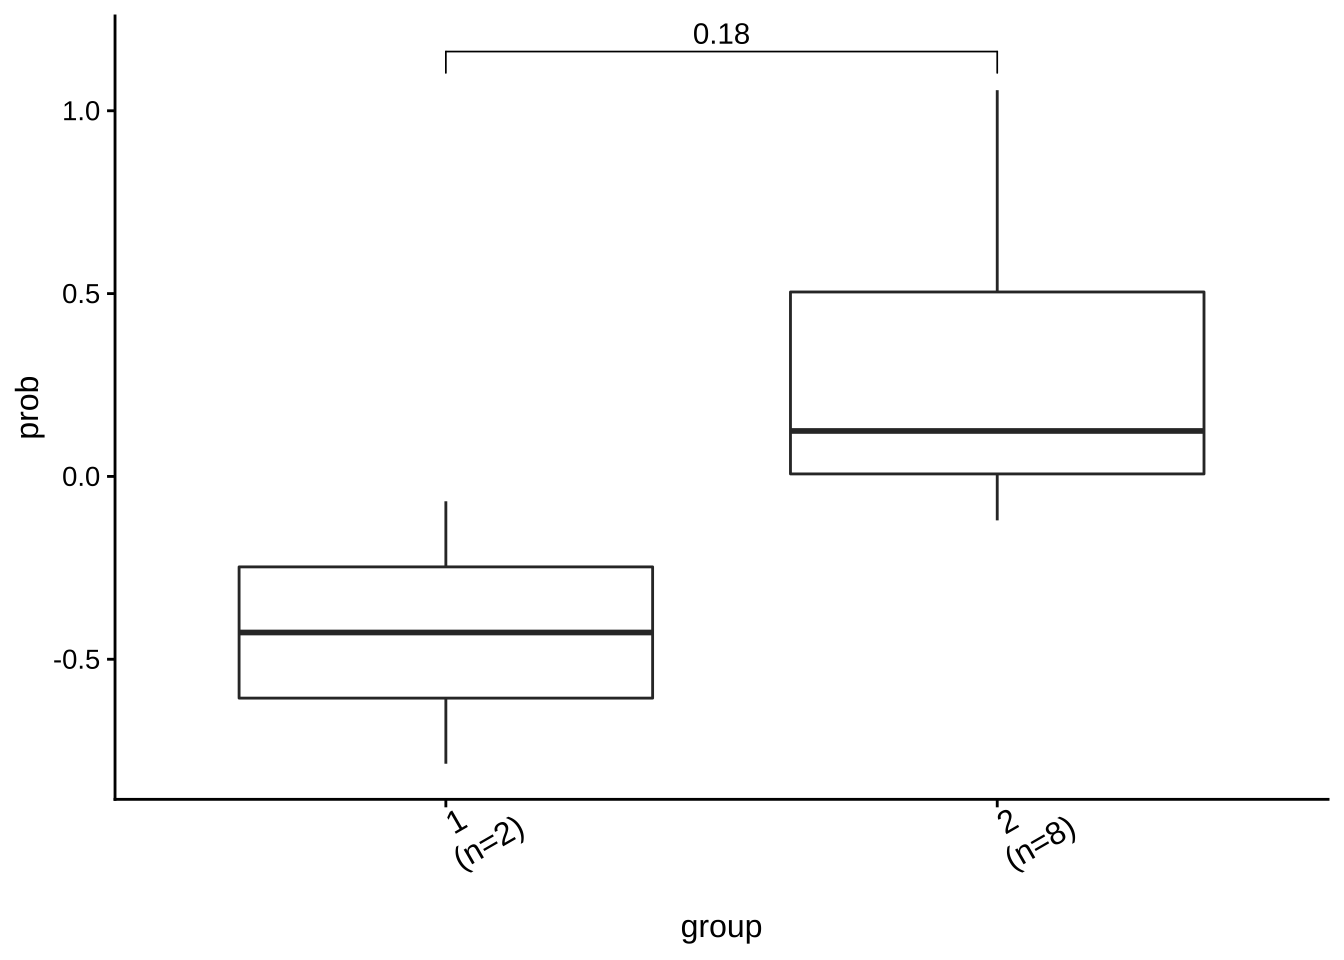
\includegraphics[width=0.95\linewidth]{sigminer_files/figure-latex/unnamed-chunk-98-1}

\begin{Shaded}
\begin{Highlighting}[]
\NormalTok{ggcomp}\SpecialCharTok{$}\NormalTok{ca\_comb}
\end{Highlighting}
\end{Shaded}

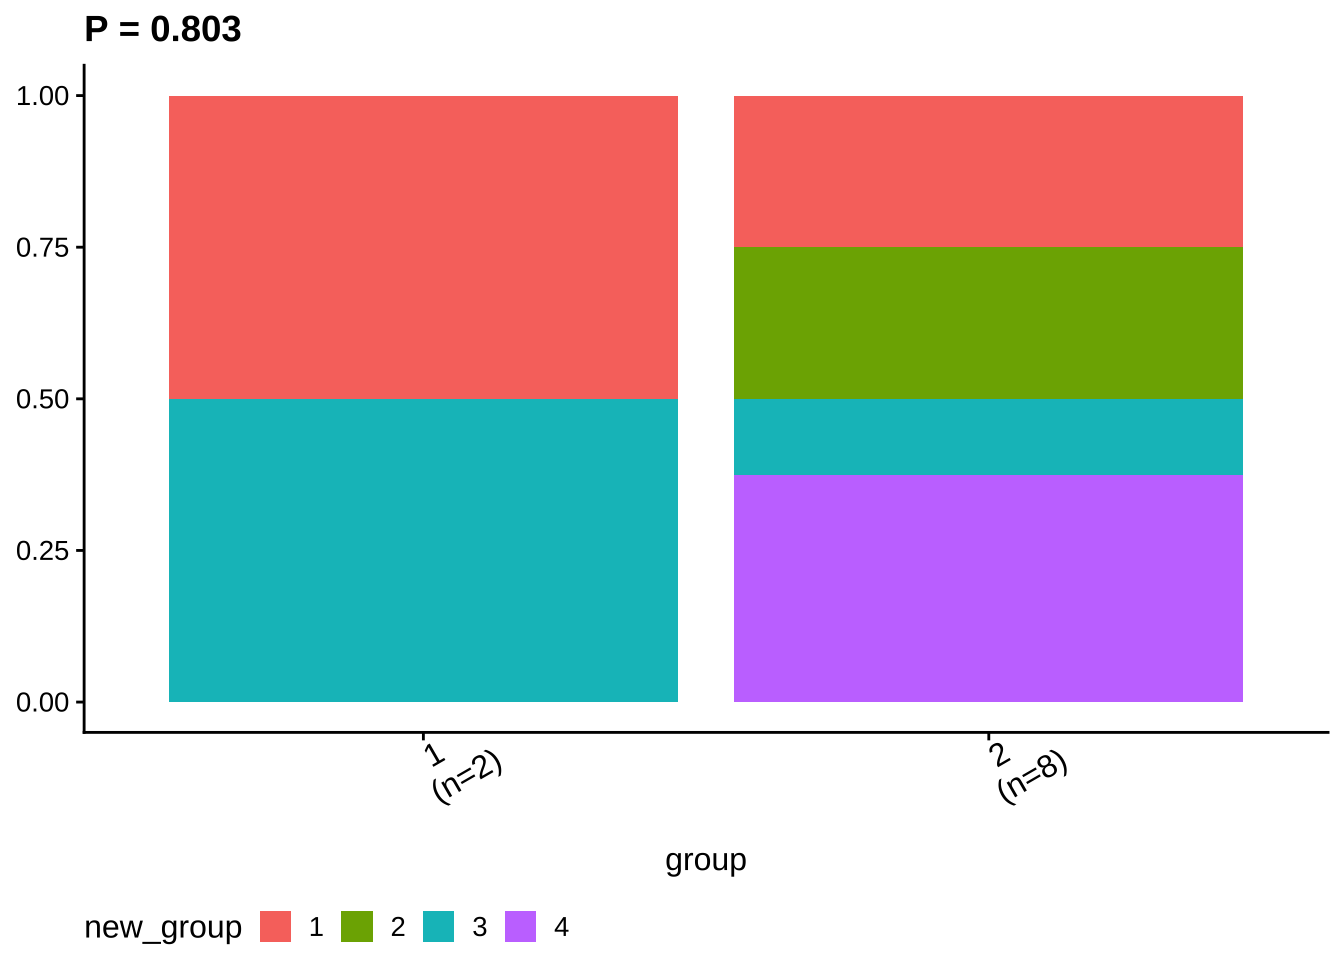
\includegraphics[width=0.95\linewidth]{sigminer_files/figure-latex/unnamed-chunk-98-2}

\hypertarget{subtype-prediction}{%
\chapter{Subtype prediction}\label{subtype-prediction}}

To expand the power of signatures to clinical application, based on signature activity, we can go further build neutral network model prediction model with \href{https://keras.io/}{\emph{keras}}. This feature is implemented in sigminer's child package \href{https://github.com/ShixiangWang/sigminer.prediction}{\textbf{sigminer.prediction}}.

If you are studying copy number signatures of prostate cancer, you can directly use the trained model, the usage has been described in the
\href{https://github.com/ShixiangWang/sigminer.prediction/blob/master/README.md}{\emph{README} file}.

For other situations, you can reuse the functions \href{https://github.com/ShixiangWang/sigminer.prediction/blob/master/R/modeling_and_fitting.R}{\texttt{modeling\_and\_fitting()}}
and \href{https://github.com/ShixiangWang/sigminer.prediction/blob/master/R/batch_modeling_and_fitting.R}{\texttt{batch\_modeling\_and\_fitting()}} (for batch processing) for building models.

\hypertarget{sigflow}{%
\chapter{Sigflow pipeline}\label{sigflow}}

\href{https://github.com/ShixiangWang/sigflow}{\textbf{Sigflow}} provides useful mutational signature analysis workflows based on R package \textbf{sigminer}. It can auto-extract mutational signatures, fit mutation data to COSMIC reference signatures (SBS/DBS/INDEL) and run bootstrapping analysis for signature fitting.

For full documentation, please read Sigflow \href{https://github.com/ShixiangWang/sigflow}{\emph{README}}.

\hypertarget{cancer-type-specific-signature-index-database}{%
\section{Cancer type specific signature index database}\label{cancer-type-specific-signature-index-database}}

Signature fitting analysis may befit from directly specifying known signatures identified in a cancer type. We collect such information and provide the following data tables.

\begin{Shaded}
\begin{Highlighting}[]
\NormalTok{db1 }\OtherTok{\textless{}{-}} \FunctionTok{system.file}\NormalTok{(}\StringTok{"extdata"}\NormalTok{, }\StringTok{"cosmic2\_record\_by\_cancer.rds"}\NormalTok{, }\AttributeTok{package =} \StringTok{"sigminer"}\NormalTok{)}
\NormalTok{db1 }\OtherTok{\textless{}{-}} \FunctionTok{readRDS}\NormalTok{(db1)}
\FunctionTok{colnames}\NormalTok{(db1) }\OtherTok{\textless{}{-}} \FunctionTok{c}\NormalTok{(}\StringTok{"Cancer type"}\NormalTok{, }\StringTok{"Signature Index"}\NormalTok{)}
\NormalTok{db2 }\OtherTok{\textless{}{-}} \FunctionTok{system.file}\NormalTok{(}\StringTok{"extdata"}\NormalTok{, }\StringTok{"signature\_record\_by\_cancer.rds"}\NormalTok{, }\AttributeTok{package =} \StringTok{"sigminer"}\NormalTok{)}
\NormalTok{db2 }\OtherTok{\textless{}{-}} \FunctionTok{readRDS}\NormalTok{(db2)}
\FunctionTok{colnames}\NormalTok{(db2) }\OtherTok{\textless{}{-}} \FunctionTok{c}\NormalTok{(}
  \StringTok{"Cancer type"}\NormalTok{, }\StringTok{"Cohort"}\NormalTok{, }\StringTok{"Sequencing strategy"}\NormalTok{,}
  \StringTok{"SBS signature index"}\NormalTok{,}
  \StringTok{"DBS signature index"}\NormalTok{,}
  \StringTok{"ID signature index"}
\NormalTok{)}
\end{Highlighting}
\end{Shaded}

\begin{Shaded}
\begin{Highlighting}[]
\NormalTok{DT}\SpecialCharTok{::}\FunctionTok{datatable}\NormalTok{(db1, }\AttributeTok{caption =} \StringTok{"Data source: https://cancer.sanger.ac.uk/signatures\_v2/matrix.png"}\NormalTok{)}
\DocumentationTok{\#\# PhantomJS not found. You can install it with webshot::install\_phantomjs(). If it is installed, please make sure the phantomjs executable can be found via the PATH variable.}
\end{Highlighting}
\end{Shaded}

\begin{quote}
Note, set \texttt{sig\_db} to `legacy' (the default) in \texttt{sig\_fit()} family functions.
\end{quote}

\begin{Shaded}
\begin{Highlighting}[]
\NormalTok{DT}\SpecialCharTok{::}\FunctionTok{datatable}\NormalTok{(db2[, }\FunctionTok{c}\NormalTok{(}\DecValTok{1}\SpecialCharTok{:}\DecValTok{3}\NormalTok{, }\DecValTok{4}\NormalTok{)], }\AttributeTok{caption =} \StringTok{"Data source: Alexandrov et al. https://www.nature.com/articles/s41586{-}020{-}1943{-}3"}\NormalTok{)}
\end{Highlighting}
\end{Shaded}

\begin{Shaded}
\begin{Highlighting}[]
\NormalTok{DT}\SpecialCharTok{::}\FunctionTok{datatable}\NormalTok{(db2[, }\FunctionTok{c}\NormalTok{(}\DecValTok{1}\SpecialCharTok{:}\DecValTok{3}\NormalTok{, }\DecValTok{5}\NormalTok{)], }\AttributeTok{caption =} \StringTok{"Data source: Alexandrov et al. https://www.nature.com/articles/s41586{-}020{-}1943{-}3"}\NormalTok{)}
\end{Highlighting}
\end{Shaded}

\begin{Shaded}
\begin{Highlighting}[]
\NormalTok{DT}\SpecialCharTok{::}\FunctionTok{datatable}\NormalTok{(db2[, }\FunctionTok{c}\NormalTok{(}\DecValTok{1}\SpecialCharTok{:}\DecValTok{3}\NormalTok{, }\DecValTok{6}\NormalTok{)], }\AttributeTok{caption =} \StringTok{"Data source: Alexandrov et al. https://www.nature.com/articles/s41586{-}020{-}1943{-}3"}\NormalTok{)}
\end{Highlighting}
\end{Shaded}

\hypertarget{datasets}{%
\chapter{Datasets}\label{datasets}}

\hypertarget{reference-annotation}{%
\section{Reference annotation}\label{reference-annotation}}

\textbf{sigminer} stores many reference annotation datasets for internal calculation. It can be exported for other usage either by \texttt{data()} or \texttt{get\_genome\_annotation()}.

Currently, there are the following datasets:

\begin{itemize}
\tightlist
\item
  \texttt{centromeres.hg19}
\item
  \texttt{centromeres.hg38}
\item
  \texttt{chromsize.hg19}
\item
  \texttt{chromsize.hg38}
\item
  \texttt{cytobands.hg19}
\item
  \texttt{cytobands.hg38}
\end{itemize}

An example is given as below:

\begin{Shaded}
\begin{Highlighting}[]
\FunctionTok{data}\NormalTok{(}\StringTok{"centromeres.hg19"}\NormalTok{)}
\FunctionTok{head}\NormalTok{(centromeres.hg19)}
\DocumentationTok{\#\#   chrom left.base right.base}
\DocumentationTok{\#\# 1  chr1 121535434  124535434}
\DocumentationTok{\#\# 2  chr2  92326171   95326171}
\DocumentationTok{\#\# 3  chr3  90504854   93504854}
\DocumentationTok{\#\# 4  chr4  49660117   52660117}
\DocumentationTok{\#\# 5  chr5  46405641   49405641}
\DocumentationTok{\#\# 6  chr6  58830166   61830166}
\end{Highlighting}
\end{Shaded}

\texttt{get\_genome\_annotation()} can better control the returned \texttt{data.frame}.

\begin{Shaded}
\begin{Highlighting}[]
\FunctionTok{get\_genome\_annotation}\NormalTok{(}
  \AttributeTok{data\_type =} \StringTok{"chr\_size"}\NormalTok{,}
  \AttributeTok{chrs =} \FunctionTok{c}\NormalTok{(}\StringTok{"chr1"}\NormalTok{, }\StringTok{"chr10"}\NormalTok{, }\StringTok{"chr20"}\NormalTok{),}
  \AttributeTok{genome\_build =} \StringTok{"hg19"}
\NormalTok{)}
\DocumentationTok{\#\#   chrom      size}
\DocumentationTok{\#\# 1  chr1 249250621}
\DocumentationTok{\#\# 2 chr10 135534747}
\DocumentationTok{\#\# 3 chr20  63025520}
\end{Highlighting}
\end{Shaded}

More see \texttt{?get\_genome\_annotation}.

\hypertarget{copy-number-components-setting}{%
\section{Copy number components setting}\label{copy-number-components-setting}}

Dataset \texttt{CN.features} is a predefined component data table for identifying copy number signatures by method ``Wang''.
Users can define a custom table with similar structure and pass it to function like \texttt{sig\_tally()}.

Detail about how to generate this dataset can be viewed at \url{https://github.com/ShixiangWang/sigminer/blob/master/data-raw/CN-features.R}.

\begin{Shaded}
\begin{Highlighting}[]
\NormalTok{CN.features}
\DocumentationTok{\#\#     feature         component label  min max}
\DocumentationTok{\#\#  1:  BP10MB         BP10MB[0] point    0   0}
\DocumentationTok{\#\#  2:  BP10MB         BP10MB[1] point    1   1}
\DocumentationTok{\#\#  3:  BP10MB         BP10MB[2] point    2   2}
\DocumentationTok{\#\#  4:  BP10MB         BP10MB[3] point    3   3}
\DocumentationTok{\#\#  5:  BP10MB         BP10MB[4] point    4   4}
\DocumentationTok{\#\#  6:  BP10MB         BP10MB[5] point    5   5}
\DocumentationTok{\#\#  7:  BP10MB        BP10MB[\textgreater{}5] range    5 Inf}
\DocumentationTok{\#\#  8:   BPArm          BPArm[0] point    0   0}
\DocumentationTok{\#\#  9:   BPArm          BPArm[1] point    1   1}
\DocumentationTok{\#\# 10:   BPArm          BPArm[2] point    2   2}
\DocumentationTok{\#\# 11:   BPArm          BPArm[3] point    3   3}
\DocumentationTok{\#\# 12:   BPArm          BPArm[4] point    4   4}
\DocumentationTok{\#\# 13:   BPArm          BPArm[5] point    5   5}
\DocumentationTok{\#\# 14:   BPArm          BPArm[6] point    6   6}
\DocumentationTok{\#\# 15:   BPArm          BPArm[7] point    7   7}
\DocumentationTok{\#\# 16:   BPArm          BPArm[8] point    8   8}
\DocumentationTok{\#\# 17:   BPArm          BPArm[9] point    9   9}
\DocumentationTok{\#\# 18:   BPArm         BPArm[10] point   10  10}
\DocumentationTok{\#\# 19:   BPArm BPArm[\textgreater{}10 \& \textless{}=20] range   10  20}
\DocumentationTok{\#\# 20:   BPArm BPArm[\textgreater{}20 \& \textless{}=30] range   20  30}
\DocumentationTok{\#\# 21:   BPArm        BPArm[\textgreater{}30] range   30 Inf}
\DocumentationTok{\#\# 22:      CN             CN[0] point    0   0}
\DocumentationTok{\#\# 23:      CN             CN[1] point    1   1}
\DocumentationTok{\#\# 24:      CN             CN[2] point    2   2}
\DocumentationTok{\#\# 25:      CN             CN[3] point    3   3}
\DocumentationTok{\#\# 26:      CN             CN[4] point    4   4}
\DocumentationTok{\#\# 27:      CN      CN[\textgreater{}4 \& \textless{}=8] range    4   8}
\DocumentationTok{\#\# 28:      CN            CN[\textgreater{}8] range    8 Inf}
\DocumentationTok{\#\# 29:    CNCP           CNCP[0] point    0   0}
\DocumentationTok{\#\# 30:    CNCP           CNCP[1] point    1   1}
\DocumentationTok{\#\# 31:    CNCP           CNCP[2] point    2   2}
\DocumentationTok{\#\# 32:    CNCP           CNCP[3] point    3   3}
\DocumentationTok{\#\# 33:    CNCP           CNCP[4] point    4   4}
\DocumentationTok{\#\# 34:    CNCP    CNCP[\textgreater{}4 \& \textless{}=8] range    4   8}
\DocumentationTok{\#\# 35:    CNCP          CNCP[\textgreater{}8] range    8 Inf}
\DocumentationTok{\#\# 36:    OsCN           OsCN[0] point    0   0}
\DocumentationTok{\#\# 37:    OsCN           OsCN[1] point    1   1}
\DocumentationTok{\#\# 38:    OsCN           OsCN[2] point    2   2}
\DocumentationTok{\#\# 39:    OsCN           OsCN[3] point    3   3}
\DocumentationTok{\#\# 40:    OsCN           OsCN[4] point    4   4}
\DocumentationTok{\#\# 41:    OsCN   OsCN[\textgreater{}4 \& \textless{}=10] range    4  10}
\DocumentationTok{\#\# 42:    OsCN         OsCN[\textgreater{}10] range   10 Inf}
\DocumentationTok{\#\# 43:      SS           SS[\textless{}=2] range {-}Inf   2}
\DocumentationTok{\#\# 44:      SS      SS[\textgreater{}2 \& \textless{}=3] range    2   3}
\DocumentationTok{\#\# 45:      SS      SS[\textgreater{}3 \& \textless{}=4] range    3   4}
\DocumentationTok{\#\# 46:      SS      SS[\textgreater{}4 \& \textless{}=5] range    4   5}
\DocumentationTok{\#\# 47:      SS      SS[\textgreater{}5 \& \textless{}=6] range    5   6}
\DocumentationTok{\#\# 48:      SS      SS[\textgreater{}6 \& \textless{}=7] range    6   7}
\DocumentationTok{\#\# 49:      SS      SS[\textgreater{}7 \& \textless{}=8] range    7   8}
\DocumentationTok{\#\# 50:      SS            SS[\textgreater{}8] range    8 Inf}
\DocumentationTok{\#\# 51:    NC50         NC50[\textless{}=2] range {-}Inf   2}
\DocumentationTok{\#\# 52:    NC50           NC50[3] point    3   3}
\DocumentationTok{\#\# 53:    NC50           NC50[4] point    4   4}
\DocumentationTok{\#\# 54:    NC50           NC50[5] point    5   5}
\DocumentationTok{\#\# 55:    NC50           NC50[6] point    6   6}
\DocumentationTok{\#\# 56:    NC50           NC50[7] point    7   7}
\DocumentationTok{\#\# 57:    NC50          NC50[\textgreater{}7] range    7 Inf}
\DocumentationTok{\#\# 58:   BoChr          BoChr[1] point    1   1}
\DocumentationTok{\#\# 59:   BoChr          BoChr[2] point    2   2}
\DocumentationTok{\#\# 60:   BoChr          BoChr[3] point    3   3}
\DocumentationTok{\#\# 61:   BoChr          BoChr[4] point    4   4}
\DocumentationTok{\#\# 62:   BoChr          BoChr[5] point    5   5}
\DocumentationTok{\#\# 63:   BoChr          BoChr[6] point    6   6}
\DocumentationTok{\#\# 64:   BoChr          BoChr[7] point    7   7}
\DocumentationTok{\#\# 65:   BoChr          BoChr[8] point    8   8}
\DocumentationTok{\#\# 66:   BoChr          BoChr[9] point    9   9}
\DocumentationTok{\#\# 67:   BoChr         BoChr[10] point   10  10}
\DocumentationTok{\#\# 68:   BoChr         BoChr[11] point   11  11}
\DocumentationTok{\#\# 69:   BoChr         BoChr[12] point   12  12}
\DocumentationTok{\#\# 70:   BoChr         BoChr[13] point   13  13}
\DocumentationTok{\#\# 71:   BoChr         BoChr[14] point   14  14}
\DocumentationTok{\#\# 72:   BoChr         BoChr[15] point   15  15}
\DocumentationTok{\#\# 73:   BoChr         BoChr[16] point   16  16}
\DocumentationTok{\#\# 74:   BoChr         BoChr[17] point   17  17}
\DocumentationTok{\#\# 75:   BoChr         BoChr[18] point   18  18}
\DocumentationTok{\#\# 76:   BoChr         BoChr[19] point   19  19}
\DocumentationTok{\#\# 77:   BoChr         BoChr[20] point   20  20}
\DocumentationTok{\#\# 78:   BoChr         BoChr[21] point   21  21}
\DocumentationTok{\#\# 79:   BoChr         BoChr[22] point   22  22}
\DocumentationTok{\#\# 80:   BoChr         BoChr[23] point   23  23}
\DocumentationTok{\#\#     feature         component label  min max}
\end{Highlighting}
\end{Shaded}

\hypertarget{convert}{%
\chapter{SBS signature conversion}\label{convert}}

Converts signatures between two representations relative to different sets of mutational opportunities. Currently, only SBS signature is supported.

\begin{Shaded}
\begin{Highlighting}[]
\CommentTok{\# Load SBS signature}
\FunctionTok{load}\NormalTok{(}\FunctionTok{system.file}\NormalTok{(}\StringTok{"extdata"}\NormalTok{, }\StringTok{"toy\_mutational\_signature.RData"}\NormalTok{,}
  \AttributeTok{package =} \StringTok{"sigminer"}\NormalTok{, }\AttributeTok{mustWork =} \ConstantTok{TRUE}
\NormalTok{))}
\CommentTok{\# Exome{-}relative to Genome{-}relative}
\NormalTok{sig\_converted }\OtherTok{\textless{}{-}} \FunctionTok{sig\_convert}\NormalTok{(sig2,}
  \AttributeTok{from =} \StringTok{"human{-}exome"}\NormalTok{,}
  \AttributeTok{to =} \StringTok{"human{-}genome"}
\NormalTok{)}
\NormalTok{sig\_converted}
\DocumentationTok{\#\#                  Sig1          Sig2          Sig3}
\DocumentationTok{\#\# A[C\textgreater{}A]A  0.000000e+00  1.283652e{-}02 2.354578e{-}204}
\DocumentationTok{\#\# A[C\textgreater{}A]C  0.000000e+00  1.866572e{-}02  0.000000e+00}
\DocumentationTok{\#\# A[C\textgreater{}A]G  0.000000e+00  1.618700e{-}03  0.000000e+00}
\DocumentationTok{\#\# A[C\textgreater{}A]T  0.000000e+00  7.572233e{-}03  0.000000e+00}
\DocumentationTok{\#\# C[C\textgreater{}A]A  0.000000e+00  1.209076e{-}02  0.000000e+00}
\DocumentationTok{\#\# C[C\textgreater{}A]C  0.000000e+00  7.032249e{-}03 1.170400e{-}133}
\DocumentationTok{\#\# C[C\textgreater{}A]G  0.000000e+00  3.839313e{-}03 1.165310e{-}269}
\DocumentationTok{\#\# C[C\textgreater{}A]T  0.000000e+00  1.166974e{-}02  0.000000e+00}
\DocumentationTok{\#\# G[C\textgreater{}A]A  0.000000e+00  1.025669e{-}02  4.089543e{-}15}
\DocumentationTok{\#\# G[C\textgreater{}A]C 2.975389e{-}296  4.002311e{-}03  0.000000e+00}
\DocumentationTok{\#\# G[C\textgreater{}A]G  4.796114e{-}02 4.527374e{-}117  0.000000e+00}
\DocumentationTok{\#\# G[C\textgreater{}A]T  0.000000e+00  5.994876e{-}03 1.669814e{-}131}
\DocumentationTok{\#\# T[C\textgreater{}A]A  0.000000e+00  3.324941e{-}96  7.673114e{-}02}
\DocumentationTok{\#\# T[C\textgreater{}A]C  0.000000e+00  1.467589e{-}02 9.720402e{-}229}
\DocumentationTok{\#\# T[C\textgreater{}A]G  0.000000e+00  3.199454e{-}03  0.000000e+00}
\DocumentationTok{\#\# T[C\textgreater{}A]T  0.000000e+00  2.338506e{-}02  0.000000e+00}
\DocumentationTok{\#\# A[C\textgreater{}G]A  0.000000e+00  1.198076e{-}02 1.210238e{-}153}
\DocumentationTok{\#\# A[C\textgreater{}G]C  0.000000e+00  3.999796e{-}03  0.000000e+00}
\DocumentationTok{\#\# A[C\textgreater{}G]G  9.976549e{-}02  7.184837e{-}58  0.000000e+00}
\DocumentationTok{\#\# A[C\textgreater{}G]T  0.000000e+00  7.572233e{-}03 9.731662e{-}108}
\DocumentationTok{\#\# C[C\textgreater{}G]A  0.000000e+00  8.732217e{-}03  1.472610e{-}34}
\DocumentationTok{\#\# C[C\textgreater{}G]C  0.000000e+00  1.875266e{-}03  0.000000e+00}
\DocumentationTok{\#\# C[C\textgreater{}G]G  0.000000e+00  4.429976e{-}03  1.144811e{-}70}
\DocumentationTok{\#\# C[C\textgreater{}G]T  1.398527e{-}01  1.003533e{-}19  0.000000e+00}
\DocumentationTok{\#\# G[C\textgreater{}G]A 1.227107e{-}293  7.521572e{-}03 2.969058e{-}285}
\DocumentationTok{\#\# G[C\textgreater{}G]C  0.000000e+00  3.001734e{-}03 2.665595e{-}168}
\DocumentationTok{\#\# G[C\textgreater{}G]G  0.000000e+00  2.178881e{-}03  0.000000e+00}
\DocumentationTok{\#\# G[C\textgreater{}G]T  0.000000e+00  3.996584e{-}03  0.000000e+00}
\DocumentationTok{\#\# T[C\textgreater{}G]A  0.000000e+00  4.493267e{-}03 2.338585e{-}311}
\DocumentationTok{\#\# T[C\textgreater{}G]C  0.000000e+00  5.336688e{-}03 1.100445e{-}248}
\DocumentationTok{\#\# T[C\textgreater{}G]G  0.000000e+00  5.027714e{-}03 2.505791e{-}283}
\DocumentationTok{\#\# T[C\textgreater{}G]T  0.000000e+00  8.094828e{-}03  4.211703e{-}12}
\DocumentationTok{\#\# A[C\textgreater{}T]A  0.000000e+00  4.278842e{-}02 6.186711e{-}285}
\DocumentationTok{\#\# A[C\textgreater{}T]C  0.000000e+00  3.266500e{-}02 4.009287e{-}180}
\DocumentationTok{\#\# A[C\textgreater{}T]G  0.000000e+00  8.943317e{-}02 1.936180e{-}271}
\DocumentationTok{\#\# A[C\textgreater{}T]T  0.000000e+00  2.366323e{-}02  0.000000e+00}
\DocumentationTok{\#\# C[C\textgreater{}T]A  0.000000e+00  2.552494e{-}02  0.000000e+00}
\DocumentationTok{\#\# C[C\textgreater{}T]C  0.000000e+00  1.406450e{-}02 1.334078e{-}226}
\DocumentationTok{\#\# C[C\textgreater{}T]G  0.000000e+00  5.463637e{-}02 9.737288e{-}158}
\DocumentationTok{\#\# C[C\textgreater{}T]T  0.000000e+00  3.695418e{-}02 4.246509e{-}172}
\DocumentationTok{\#\# G[C\textgreater{}T]A  0.000000e+00 1.550033e{-}134  1.379990e{-}01}
\DocumentationTok{\#\# G[C\textgreater{}T]C  0.000000e+00  2.401387e{-}02 9.655208e{-}197}
\DocumentationTok{\#\# G[C\textgreater{}T]G  0.000000e+00  5.665090e{-}02 1.322415e{-}193}
\DocumentationTok{\#\# G[C\textgreater{}T]T  0.000000e+00  3.197267e{-}02 1.483309e{-}124}
\DocumentationTok{\#\# T[C\textgreater{}T]A  0.000000e+00  3.504749e{-}02 1.602583e{-}125}
\DocumentationTok{\#\# T[C\textgreater{}T]C  0.000000e+00  2.868470e{-}02 2.192251e{-}133}
\DocumentationTok{\#\# T[C\textgreater{}T]G  0.000000e+00  5.607061e{-}45  3.725237e{-}01}
\DocumentationTok{\#\# T[C\textgreater{}T]T  0.000000e+00  2.248563e{-}02 5.991874e{-}150}
\DocumentationTok{\#\# A[T\textgreater{}A]A  0.000000e+00 8.169022e{-}163 4.909543e{-}207}
\DocumentationTok{\#\# A[T\textgreater{}A]C  0.000000e+00  9.451235e{-}03 9.169290e{-}161}
\DocumentationTok{\#\# A[T\textgreater{}A]G  0.000000e+00 1.860257e{-}209  3.781700e{-}02}
\DocumentationTok{\#\# A[T\textgreater{}A]T  0.000000e+00  3.646724e{-}03  0.000000e+00}
\DocumentationTok{\#\# C[T\textgreater{}A]A  0.000000e+00  9.626354e{-}63 1.877035e{-}152}
\DocumentationTok{\#\# C[T\textgreater{}A]C  0.000000e+00  4.098575e{-}03  8.954807e{-}03}
\DocumentationTok{\#\# C[T\textgreater{}A]G  0.000000e+00  7.584736e{-}03  1.779246e{-}46}
\DocumentationTok{\#\# C[T\textgreater{}A]T  0.000000e+00  4.886651e{-}03  0.000000e+00}
\DocumentationTok{\#\# G[T\textgreater{}A]A  0.000000e+00 1.923466e{-}257  1.645056e{-}02}
\DocumentationTok{\#\# G[T\textgreater{}A]C  0.000000e+00  5.990275e{-}03 2.816093e{-}138}
\DocumentationTok{\#\# G[T\textgreater{}A]G  0.000000e+00  2.491146e{-}03 5.966918e{-}137}
\DocumentationTok{\#\# G[T\textgreater{}A]T  1.780073e{-}01 1.470587e{-}107  0.000000e+00}
\DocumentationTok{\#\# T[T\textgreater{}A]A  0.000000e+00  0.000000e+00  1.576605e{-}78}
\DocumentationTok{\#\# T[T\textgreater{}A]C  0.000000e+00 3.652510e{-}193  3.025830e{-}02}
\DocumentationTok{\#\# T[T\textgreater{}A]G  0.000000e+00  0.000000e+00  3.102984e{-}02}
\DocumentationTok{\#\# T[T\textgreater{}A]T  0.000000e+00  5.570191e{-}03 2.661350e{-}186}
\DocumentationTok{\#\# A[T\textgreater{}C]A  0.000000e+00  3.673499e{-}02 2.037390e{-}236}
\DocumentationTok{\#\# A[T\textgreater{}C]C  0.000000e+00  4.875997e{-}80  8.069896e{-}02}
\DocumentationTok{\#\# A[T\textgreater{}C]G  0.000000e+00  2.533400e{-}02 4.653276e{-}300}
\DocumentationTok{\#\# A[T\textgreater{}C]T  0.000000e+00  3.403610e{-}02 1.137147e{-}235}
\DocumentationTok{\#\# C[T\textgreater{}C]A  0.000000e+00  7.619558e{-}03  1.273356e{-}94}
\DocumentationTok{\#\# C[T\textgreater{}C]C  0.000000e+00  1.116095e{-}02 1.501723e{-}122}
\DocumentationTok{\#\# C[T\textgreater{}C]G  0.000000e+00  9.506418e{-}50  9.321794e{-}02}
\DocumentationTok{\#\# C[T\textgreater{}C]T  0.000000e+00  1.172796e{-}02  1.679251e{-}87}
\DocumentationTok{\#\# G[T\textgreater{}C]A  0.000000e+00  4.585040e{-}03  5.536247e{-}03}
\DocumentationTok{\#\# G[T\textgreater{}C]C  0.000000e+00 5.073564e{-}255  4.133148e{-}02}
\DocumentationTok{\#\# G[T\textgreater{}C]G  0.000000e+00  6.850650e{-}03  0.000000e+00}
\DocumentationTok{\#\# G[T\textgreater{}C]T  3.036787e{-}50  1.058999e{-}02 7.624782e{-}161}
\DocumentationTok{\#\# T[T\textgreater{}C]A  0.000000e+00 1.774320e{-}183  1.917769e{-}02}
\DocumentationTok{\#\# T[T\textgreater{}C]C 3.471970e{-}224  7.796288e{-}03  0.000000e+00}
\DocumentationTok{\#\# T[T\textgreater{}C]G  0.000000e+00  9.993850e{-}03  0.000000e+00}
\DocumentationTok{\#\# T[T\textgreater{}C]T  0.000000e+00  2.116673e{-}02 4.729625e{-}249}
\DocumentationTok{\#\# A[T\textgreater{}G]A  0.000000e+00  6.559820e{-}03  0.000000e+00}
\DocumentationTok{\#\# A[T\textgreater{}G]C  0.000000e+00 8.576821e{-}159  1.467254e{-}02}
\DocumentationTok{\#\# A[T\textgreater{}G]G  0.000000e+00  1.544237e{-}03  3.140069e{-}03}
\DocumentationTok{\#\# A[T\textgreater{}G]T  0.000000e+00  3.646724e{-}03  0.000000e+00}
\DocumentationTok{\#\# C[T\textgreater{}G]A  0.000000e+00  1.088508e{-}03  0.000000e+00}
\DocumentationTok{\#\# C[T\textgreater{}G]C  0.000000e+00  5.252213e{-}03 5.352907e{-}111}
\DocumentationTok{\#\# C[T\textgreater{}G]G  0.000000e+00  6.320613e{-}03  0.000000e+00}
\DocumentationTok{\#\# C[T\textgreater{}G]T  1.505897e{-}01  2.544085e{-}94 2.345935e{-}218}
\DocumentationTok{\#\# G[T\textgreater{}G]A  9.796461e{-}02  2.199487e{-}93 1.446688e{-}154}
\DocumentationTok{\#\# G[T\textgreater{}G]C  0.000000e+00  1.996758e{-}03  0.000000e+00}
\DocumentationTok{\#\# G[T\textgreater{}G]G  0.000000e+00  3.736718e{-}03  0.000000e+00}
\DocumentationTok{\#\# G[T\textgreater{}G]T  0.000000e+00  3.701349e{-}72  1.494581e{-}02}
\DocumentationTok{\#\# T[T\textgreater{}G]A  1.142049e{-}01 5.198170e{-}158  0.000000e+00}
\DocumentationTok{\#\# T[T\textgreater{}G]C  0.000000e+00  4.872680e{-}03  0.000000e+00}
\DocumentationTok{\#\# T[T\textgreater{}G]G  0.000000e+00  1.798724e{-}19  1.551492e{-}02}
\DocumentationTok{\#\# T[T\textgreater{}G]T  1.716541e{-}01  1.775134e{-}54  0.000000e+00}
\FunctionTok{show\_sig\_profile}\NormalTok{(sig2, }\AttributeTok{style =} \StringTok{"cosmic"}\NormalTok{)}
\end{Highlighting}
\end{Shaded}

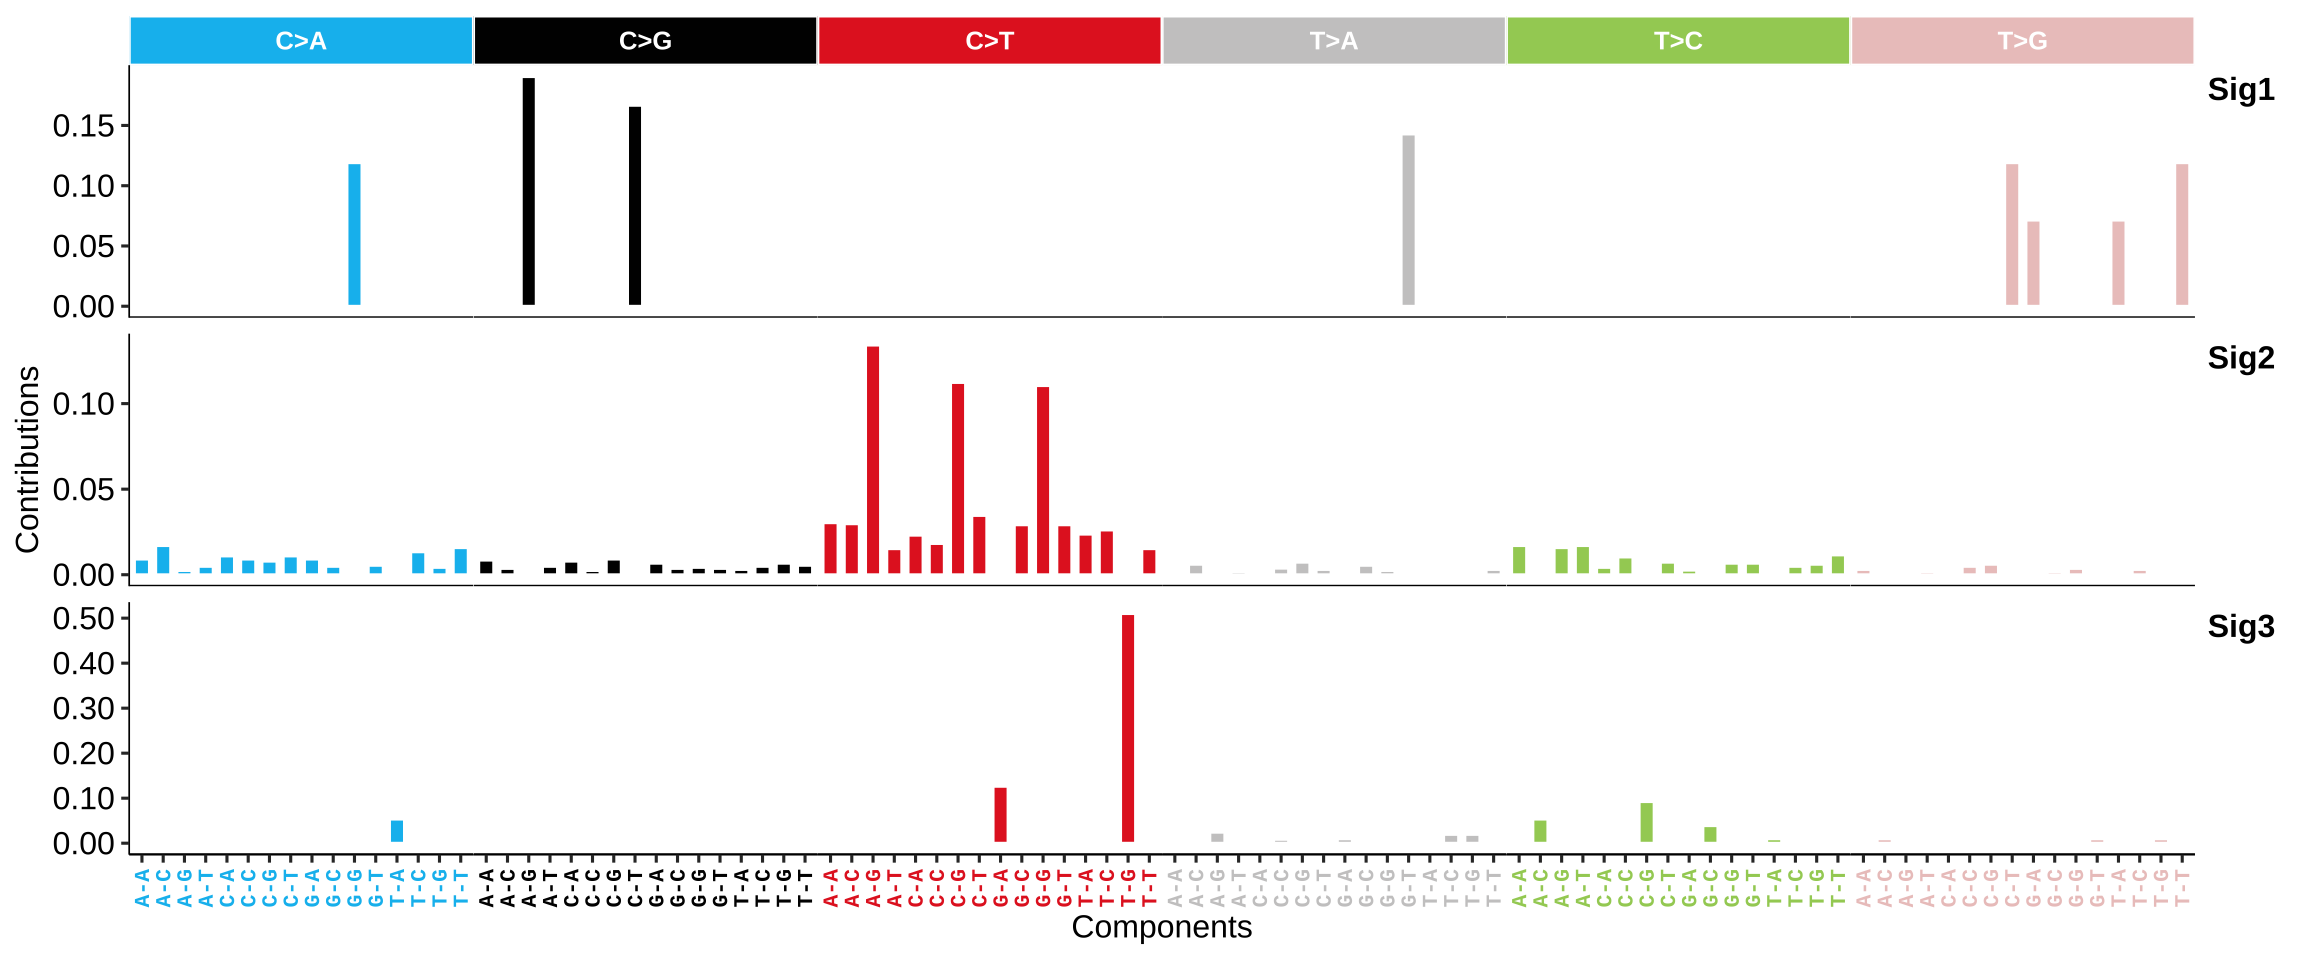
\includegraphics[width=0.95\linewidth]{sigminer_files/figure-latex/unnamed-chunk-107-1}

\begin{Shaded}
\begin{Highlighting}[]
\FunctionTok{show\_sig\_profile}\NormalTok{(sig\_converted, }\AttributeTok{style =} \StringTok{"cosmic"}\NormalTok{)}
\end{Highlighting}
\end{Shaded}

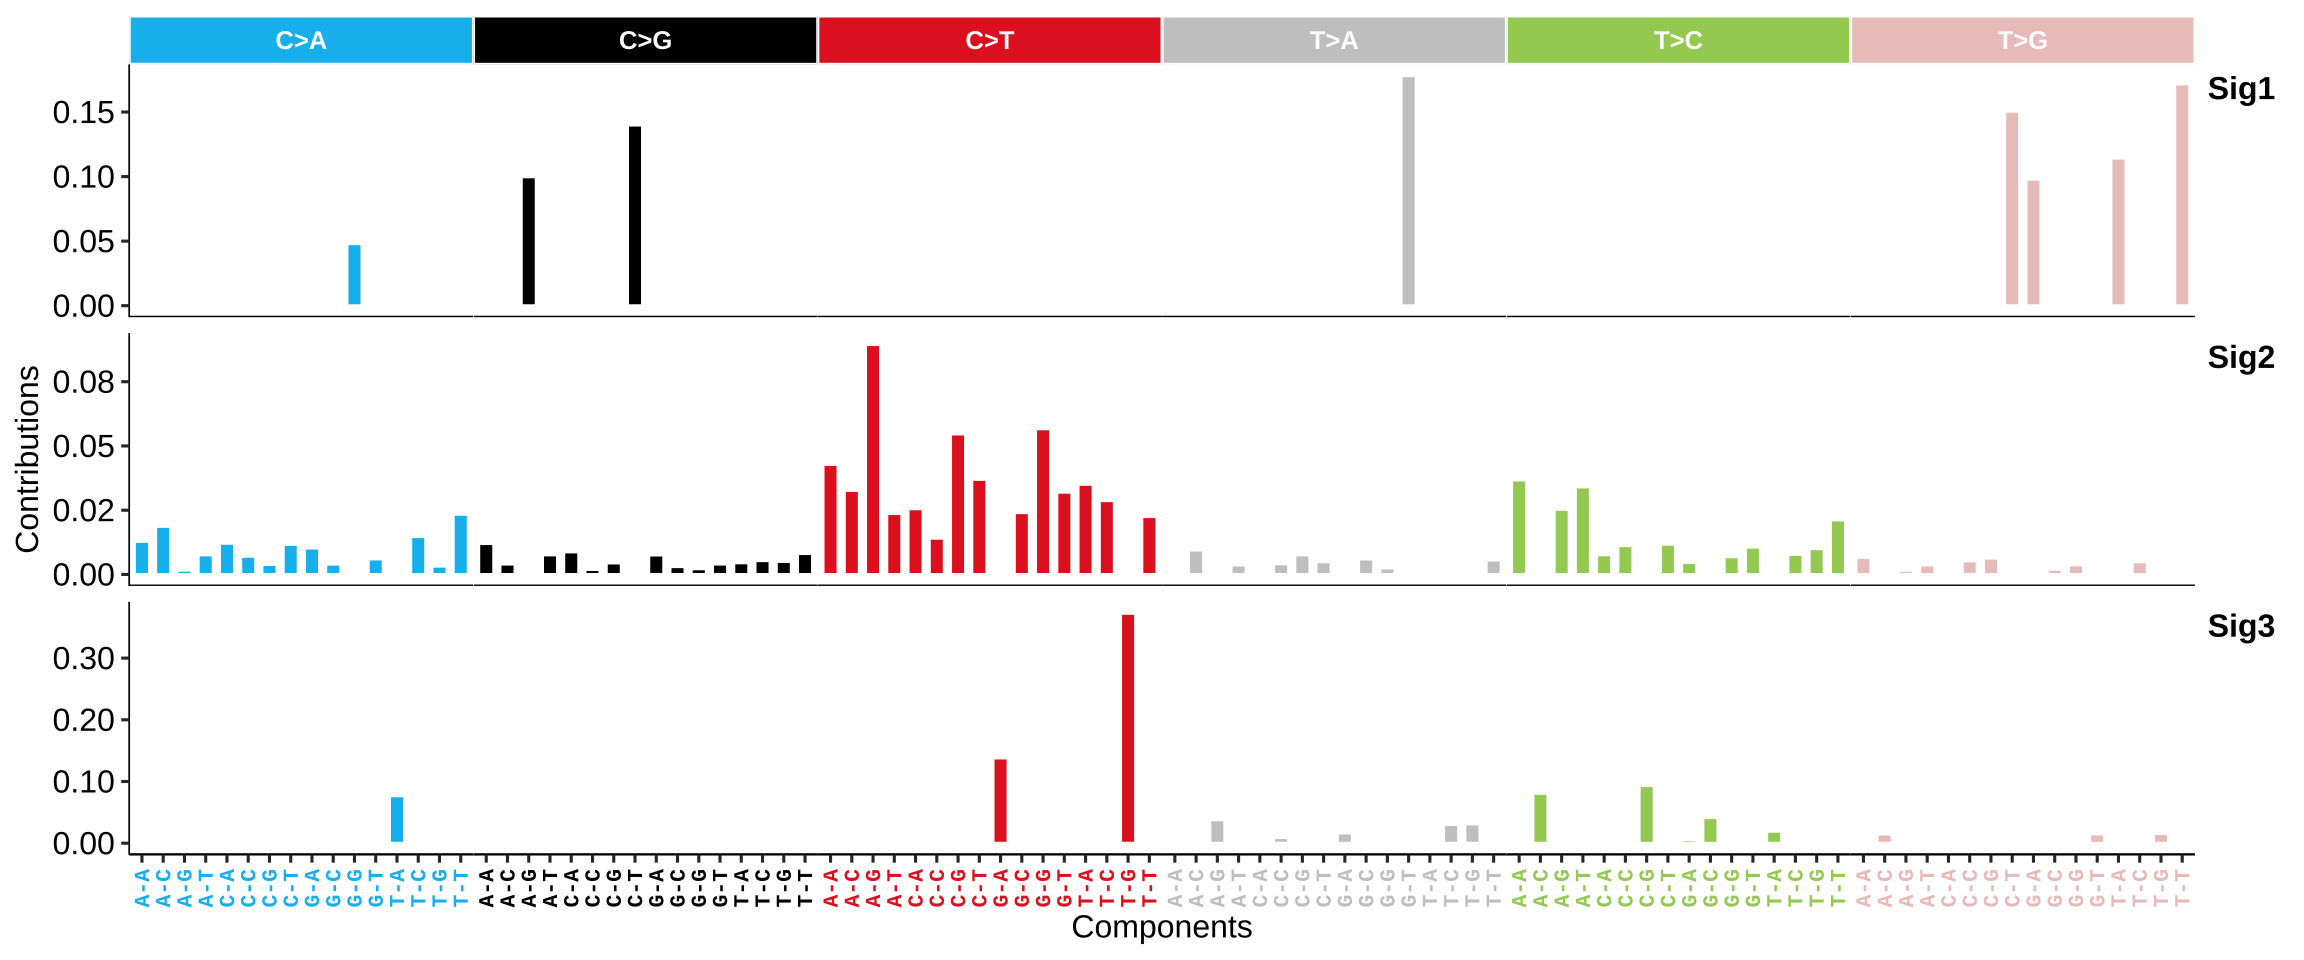
\includegraphics[width=0.95\linewidth]{sigminer_files/figure-latex/unnamed-chunk-107-2}

\hypertarget{appendix-appendix}{%
\appendix \addcontentsline{toc}{chapter}{\appendixname}}


  \bibliography{book.bib}

\end{document}
